\documentclass[twoside,11pt]{article}

% Any additional packages needed should be included after jmlr2e.
% Note that jmlr2e.sty includes epsfig, amssymb, natbib and graphicx,
% and defines many common macros, such as 'proof' and 'example'.
%
% It also sets the bibliographystyle to plainnat; for more information on
% natbib citation styles, see the natbib documentation, a copy of which
% is archived at http://www.jmlr.org/format/natbib.pdf

% Available options for package jmlr2e are:
%
%   - abbrvbib : use abbrvnat for the bibliography style
%   - nohyperref : do not load the hyperref package
%   - preprint : remove JMLR specific information from the template,
%         useful for example for posting to preprint servers.
%
% Example of using the package with custom options:
%
% \usepackage[abbrvbib, preprint]{jmlr2e}

\usepackage{jmlr2e}

% Definitions of handy macros can go here
\usepackage{xr} 


\usepackage[english]{babel}
%\usepackage[square, numbers]{natbib}
\bibliographystyle{abbrvnat}
\setcitestyle{authoryear,open={(},close={)}}

\usepackage[utf8]{inputenc}
\usepackage{amsmath}
\usepackage{amssymb}
%\usepackage{amsthm}
%\let\proof\relax
%\let\endproof\relax
\usepackage{physics}
\usepackage{gensymb}
\usepackage{verbatim}
\usepackage{amsfonts}
\usepackage{mathrsfs}
\usepackage{tikz-cd}
\usepackage{graphicx}
\usepackage{grffile} % Added to handle dots in name of images
\usepackage{microtype}
\usepackage{centernot}
\usepackage{mathtools}
% \usepackage{algpseudocode}
\usepackage{bm}
\usepackage{caption}
\usepackage{enumitem}
\usepackage{cleveref}
\usepackage{subcaption}
\usepackage{algorithm, algpseudocode}
\usepackage{algorithmicx}

\usepackage{pgfplots}
\pgfplotsset{compat=newest}
\usepackage{tikz}
\usetikzlibrary{shapes, positioning, quotes, matrix}


\pgfplotsset{height=8cm, width=15cm,compat=1.9}

\newcommand{\dataset}{{\cal D}}
\newcommand{\fracpartial}[2]{\frac{\partial #1}{\partial  #2}}
 \DeclareMathOperator*{\esssup}{ess\,sup}
 \DeclareMathOperator*{\argmin}{arg\,min}
 \DeclareMathOperator*{\argmax}{arg\,max}
\newcommand{\Ex}{\mathbb{E}}
\newcommand{\R}{\mathbb{R}}
\newcommand{\N}{\mathbb{N}}
\newcommand*\diff{\mathop{}\!\mathrm{d}}
\newcommand*\Diff[1]{\mathop{}\!\mathrm{d^#1}}
\newcommand{\w}{{\bf w}}
\newcommand{\bellman}{\mathcal{T}}
\newcommand{\statespace}{\mathcal{S}}
\newcommand{\actionspace}{\mathcal{A}}
\newcommand{\rewardfunction}{r}
\newcommand{\vpi}{V^\pi}
\newcommand{\qpi}{Q^\pi}
\newcommand{\qstar}{Q^*}
\newcommand{\vstar}{V^*}
\newcommand{\Qhat}{{Q}}
\newcommand{\functionspace}{\mathcal{F}}
\newcommand{\KL}{\mathrm{KL}}
\newcommand{\policyparams}{\theta}
\newcommand{\boltzmannQ}{\mathcal{B}Q}
\newcommand{\entropy}{\mathcal{H}}
\newcommand{\pinew}{{\pi_\mathrm{new}}}
\newcommand{\piold}{{\pi_\mathrm{old}}}

%\newtheorem{definition}{Definition}
%\newtheorem{exercise}{Exercise}
%\newtheorem{theorem}{Theorem}
%\newtheorem{proposition}{Proposition}
%\newtheorem{example}{Example}
%\newtheorem{lemma}{Lemma}
%\newtheorem{corollary}{Corollary}

\newcommand{\martha}[1]{{\color{blue} #1 }}
\newcommand{\defeq}{:=}
\newcommand{\myparagraph}[1]{\textbf{#1} \ \ \ }

% Heading arguments are {volume}{year}{pages}{date submitted}{date published}{paper id}{author-full-names}

\jmlrheading{1}{2020}{x-xx}{x/xx}{xx/xx}{xxx}{Author1, Author2, and Author3}

% Short headings should be running head and authors last names

\ShortHeadings{Greedification Operators for Policy Optimization}{Chan, Lim, and White}
\firstpageno{1}

\begin{document}

\title{Greedification Operators for Policy Optimization: Investigating Forward and Reverse KL Divergences}

\author{\name Alan Chan \email achan4@ualberta.ca \\
        \name Sungsu Lim \email sungsu@ualberta.ca \\
        \name Martha White \email whitem@ualberta.ca \\
       \addr RLAI Laboratory\\
       University of Alberta\\
       Edmonton, Alberta, Canada
       }

\editor{Editors}

\maketitle

\begin{abstract}%   <- trailing '%' for backward compatibility of .sty file
Policy gradient methods typically estimate both explicit policy and value functions. The long-extant view of policy gradient methods as approximate policy iteration---alternating between policy evaluation and policy improvement by greedification---is a helpful framework to elucidate algorithmic choices. Effective policy evaluation under function approximation is being actively investigated; approximate greedification, however, has yet to be systematically explored. 
In this work, we highlight and investigate the difference between the forward and reverse KL divergences when used for policy improvement. We show that the reverse KL has stronger theoretical guarantees for policy improvement, but that the forward KL can also induce improvement under additional assumptions. Finally, on both small-scale and large-scale experiments, we empirically analyze the behaviour and practical performance of these variants. We observe few consistent differences between the reverse and forward KLs on discrete-action spaces, but relatively more substantial stability and convergence differences emerge on continuous-action spaces.
\end{abstract}

\begin{keywords}
  Reinforcement Learning, Policy Gradient, Policy Iteration, KL Divergence
\end{keywords}

\section{Introduction}

In policy optimization, an explicit parameterized policy is learned to approximate the optimal policy. The most common methods are policy gradient (PG) methods, which iteratively update the policy parameter using the gradient of either the discounted return or the average reward, given by the {policy gradient theorem} \citep{sutton2000policy}.
Although not a recent invention, with early work introducing Actor-Critic \citep{sutton1984}, policy gradient methods have recently seen a surge of renewed interest given their ease of application in high-dimensional, continuous action spaces when combined with neural networks \citep{schulman2015high,wang2016sample}. Many recent developments include learning deterministic polices \citep{silver2014deterministic,lillicrap2015continuous}, trust-regions \citep{schulman2015trust,schulman2017proximal}, continuous-action extensions of Q-learning \citep{ haarnoja2017reinforcement,lim2018actor,ryu2019caql}, probabilistic approaches \citep{abdolmaleki2018maximum,fellows2019virel}, and entropy regularization \citep{haarnoja2017reinforcement, haarnoja2018soft}.

One way to navigate this proliferation is to revisit the insight that many policy gradient methods can be seen as approximate policy iteration (API). To find an optimal policy, API methods \citep{bertsekas2011approximate,scherrer2014approximate} interleave approximate policy evaluation---the estimation of value functions---and (approximate) policy improvement, where the policy is greedified with respect to the action-values. Numerous papers have linked PG methods to policy iteration \citep{sutton2000policy,kakade2002approximately,perkins2002existence,perkins2003convergent,wagner2011reinterpretation,wagner2013optimistic,scherrer2014local,bhandari2019global}, including recent work connecting maximum-entropy policy gradient and value-based methods \citep{o2016combining,nachum2017bridging, schulman2017equivalence, nachum2019algaedice}.
The connection between PG and \emph{Approximate} PI arises because parameterized policies only allow for approximate greedification. For exact policies, greedification is straightforward: the policy is set to the maximal action for the approximate action-values, for each state. 
For parameterized policies, however, this is rarely possible. One option is to minimize distance to a Boltzmann distribution on the action-values \citep{wagner2011reinterpretation}, such as with a reverse KL divergence \citep{haarnoja2018soft} or a forward KL divergence \citep{vieillard2019deep}.

In this work, we investigate how one should perform the greedification step for parameterized policies. In particular, for a given action-value estimate, we investigate the difference between using a forward and reverse KL divergence, with and without entropy regularization. 

Despite the fact that both have been used, there is little investigation into the differences between these two choices; the reverse KL is the typical default. The reverse KL without entropy regularization corresponds to a standard Actor-Critic update and is easy to compute. More recently, it was shown that the reverse KL guarantees policy improvement when the KL can be minimized separately for each state \citep[p.~4]{haarnoja2018soft}. At the same time, reverse KL objectives have known problems, primarily that they are non-convex, even in an ideal case with a linear Boltzmann policy. For contextual bandits, \citet{chen2019surrogate} showed improved performance when using a surrogate, forward KL objective for the smoothed risk. The forward KL divergence is also used in supervised learning, in the form of the cross-entropy loss. It remains unclear which of the two objectives is superior for greedification.


We provide some clarity on this question in this work, with the following contributions. First, we highlight four choices for greedication: forward or reverse KL to a Boltzmann distribution on the action-values, with or without entropy regularization. 
Second, we provide several theoretical insights into policy improvement for forward and reverse KLs. We highlight that the policy improvement result for the reverse KL extends to certain function-approximation settings, and provide a counterexample where optimizing for the forward KL can fail to induce policy improvement. Nevertheless, we show that under some additional conditions, optimizing for the forward KL can induce policy improvement.  Finally, we empirically investigate the behaviour of the reverse and forward KL, with varying levels of entropy regularization, providing some evidence that the reverse KL can converge faster, but can sometimes converge to worse solutions than the forward KL, particularly under continuous actions. 


\section{Problem Formulation}

We formalize the reinforcement learning \citep{sutton2018reinforcement} problem as a {Markov Decision Process} (MDP), a tuple $(\statespace, \actionspace, \gamma, r, p)$ where $\statespace$ is the state space; $\actionspace$ is the action space; $\gamma \in [0,1]$ is the discount factor; $r : \statespace \times \actionspace \to \R$ is the reward function; and for every $(s, a) \in \statespace \times \actionspace$, $p(\cdot \mid s, a)$ gives the conditional transition probabilities over $\statespace$. 

A \textit{policy} is a mapping $\pi : \statespace \to \Delta_\actionspace$, where $\Delta_\actionspace$ is the space of probability distributions over $\actionspace$. 
%
At every discrete time step $t$, an RL agent observes a state $s_t$, from which it draws an action from its policy: $a_t \sim \pi(\cdot \mid s_t)$. The agent sends the action $a_t$ to the environment, from which it receives the reward signal $r(s_t, a_t)$ and the next state $s_t$. 

A common objective in policy optimization is the value function $V^{\pi_\theta}$ averaged over a distribution $\rho_0$ over starting states: 
\begin{align*}
J(\policyparams) \defeq \int_{\statespace} \rho_0(s) \int_{\actionspace} \pi_\policyparams(a | s) Q^{\pi_\policyparams}(s, a) \, da \, ds,
\end{align*}
where the action value is $Q^{\pi}(s,a) \defeq \Ex_{\pi, p}\left[ \sum_{k = 0}^\infty \gamma^k r(S_k, A_k) \mid S_0 = s, A_0 = a \right]$.


The {policy gradient theorem} gives us the gradient of $J(\policyparams)$ \citep{sutton2000policy},
\begin{align}\label{eq:policy-gradient-thm}
    \nabla_\policyparams J(\policyparams) &= \int_{\statespace} d^{\pi_\policyparams}(s) \int_{\actionspace} Q^{\pi_\policyparams}(s, a) \nabla_\policyparams \pi_\policyparams(a \mid s),
\end{align}
%
where $d^{\pi_\policyparams}(s) \defeq \!\sum_{t = 0}^\infty \!\gamma^t \Pr(s_t = s \!\mid\! s_0\! \sim \rho_0\!)$ is the \textit{unnormalized discounted state visitation distribution}. 

Because we do not have access to $Q^{\pi_\policyparams}$, approximations are used instead. 
Commonly, a biased but lower-variance choice is to use a learned estimate $\Qhat$ of $Q^{\pi_\policyparams}$, obtained through policy evaluation algorithms like SARSA \citep{sutton2018reinforcement}. In these Actor-Critic algorithms, the actor---the policy---updates with a (biased) estimate of the above gradient, given by this $\Qhat$---the critic. 

This procedure can be interpreted as Approximate Policy Iteration (API). API methods alternate between approximate policy evaluation to obtain a new $\Qhat$ and approximate greedification to get a policy $\pi$ that is more greedy with respect to $\Qhat$. As we show in the next section, the gradient in Equation \eqref{eq:policy-gradient-thm} can be recast as the gradient of a KL divergence to a policy peaked at maximal actions under $\Qhat$; reducing this KL updates the policy to increase its own probabilities of these maximal actions, and so become more greedy with respect to $\Qhat$. Under this view, we obtain a clear separation between estimating $\Qhat$ and greedifying $\pi$. We can be agnostic to the strategy for updating $\Qhat$---we can even use soft action values \citep{ziebart2010modeling} or Q-learning \citep{watkins1992q}---and focus on answering: for a given $\Qhat$, how can we perform an approximate greedification step and which approaches are most effective? 
   
\section{Approximate Greedification with KL Divergences}\label{sec:sac}

In this section, we discuss the use of KL Divergences to perform approximate greedification. We outline four possible options: (1) forward KL and reverse KL and (2) with or without entropy regularization. We show that many PG variants can be seen as API with the greedification step as an instance of one of these four choices. A categorization of PG variants is given in Appendix A. 

\textbf{KL Divergences}

Given two probability distributions $p, q$ on $\actionspace$, the KL divergence between $p$ and $q$ is defined as $ \KL(p \parallel q) \defeq \int_\actionspace p(a) \log\frac{p(a)}{q(a)}\, da$,
%
where $p$ is assumed to be {absolutely continuous} \citep{billingsley2008probability} with respect to $q$, to ensure that the KL divergence exists. 
%
The KL divergence is not symmetric. This asymmetry leads to the two possible choices for measuring differences between distributions: the reverse KL and the forward KL. Assume that $p$ is a true distribution that we would like to match with our learned distribution $q_\theta$, where  $q$ is smooth with respect to $\theta \in \R^k$. The \textit{forward} KL divergence is $\KL(p \parallel q_\theta)$ and the \textit{reverse} KL divergence is $\KL(q_\theta \parallel p)$. 


\textbf{Approximate Greedification}

Either KL divergence could be used for greedification of $\pi$ at a given state $s$ by setting $q_\theta = \pi_\policyparams(\cdot | s)$ and $p =  \boltzmannQ(s, \cdot)$, where $\boltzmannQ$ is defined by $\boltzmannQ(s, a) \propto \exp(\Qhat(s, a)\tau^{-1})$.
%
$\boltzmannQ$ provides the optimal (soft) greedification w.r.t. $\Qhat$. To understand why, we define the soft value functions \citep{ziebart2010modeling}, where an entropy term $\entropy(\pi(\cdot \mid s))$ is added to the reward. $V^{\pi}_{soft}(s) \defeq  \Ex_\pi\left[ \sum_{k = 0}^\infty \gamma^k \left[ r(S_k, A_k) + \tau \entropy(\pi(\cdot|S_k))\right] \mid S_0 = s \right]$. We can also define the soft action-value: $Q^{\pi}_{soft}(s,a) \defeq  \Ex_\pi\left[ r(S_0, A_0) + \gamma \Ex_{S_1}[V(S_1)] \mid S_0 = s, A_0 = a \right]$.

If we set $\pi'(\cdot | s) = \boltzmannQ(s, \cdot)$ for all $s \in \statespace$, then $Q^{\pi'}_{soft}(s,a) \ge Q^{\pi}_{soft}(s,a)$ for all $(s,a)$ \citep[Theorem 4]{haarnoja2017reinforcement}. As $\tau$ approaches zero, $Q^{\pi}_{soft}(s,a)$ approaches $Q^{\pi'}(s,a)$, and so this result generally motivates using $\boltzmannQ$ as a target policy for greedification. The KL divergences are non-negative and are zero iff $\pi'(\cdot \mid s) = \boltzmannQ(s, \cdot)$ almost everywhere.  

Define the (scaled) \textbf{Reverse KL} for greedification at a given state $s$ and action-value $\Qhat$:%, with corresponding gradient, as
%
\begin{align*}
 \text{RKL}(\policyparams; s, \Qhat) &\defeq \tau\KL\left( \pi_\policyparams(\cdot \mid s_t) \parallel \boltzmannQ(s_t, \cdot) \right) \propto -\tau\entropy(\pi_\policyparams(\cdot \mid s)) - \int_\actionspace  \pi_\policyparams(a \mid s) {Q(s, a)}\, da 
    %\nabla_\policyparams \text{RKL}(\policyparams; s, \Qhat)
    %&= -\tau\nabla_\policyparams \entropy(\pi_\policyparams(\cdot \mid s)) - \int_\actionspace \nabla_\policyparams \pi_\policyparams(a \mid s) {Q(s, a)}\, da \nonumber
\end{align*}
%
The scaling with $\tau$ is used to make the magnitude of the KL more consistent across different choices of $\tau$; the optimal value with or without the scaling is the same. 
Notice that $\tau$ plays the role of an entropy regularization parameter: a larger $\tau$ results in more entropy regularization on $\pi_\policyparams(\cdot \mid s)$.
We can take a limiting case with no entropy regularization to get the \textbf{Hard Reverse KL}.
%
\begin{align}\label{eq:hard-reverse-KL}
    \text{Hard RKL}(\policyparams; s, \Qhat) \defeq \lim_{\tau \to 0} \text{RKL}(\policyparams; s, \Qhat) &= -\int_\actionspace \pi_\theta(a \mid s) Q(s, a)\, da
\end{align}
% AC: this result is somewhat mentioned on page 6 here: https://arxiv.org/pdf/1702.08892.pdf
The gradient of \Cref{eq:hard-reverse-KL} is exactly the inner term of the policy gradient in \Cref{eq:policy-gradient-thm}! 
This means that the typical policy gradient update in actor-critic can be thought of as a greedification step with a hard reverse KL. This correspondence is maintained even when averaging across all states for the full greedification objective, as discussed in Appendix B.

Similarly, we can define the \textbf{Forward KL} for greedification %at a given state $s$ and action-value $\Qhat$: %this time omitting the entropy term which does not involve $\policyparams$
%
% AC: not sure why there are two equations for the forward KL
\begin{align}
\text{FKL}(\policyparams; s, \Qhat) &\defeq  %-\tau \int_\actionspace \boltzmannQ(s, a) \log \pi_\policyparams(a \mid s)\, da \\
    %&\propto \tau\entropy(\boltzmannQ(s, \cdot)) - \tau \int_\actionspace \boltzmannQ(s, a) \log \pi_\policyparams(a \mid s)\, da = 
    \KL\left(\boltzmannQ(s, \cdot)  \parallel \pi_\policyparams(\cdot \mid s) \right)\nonumber%\\
%\nabla_\policyparams \text{FKL}(\policyparams; s, \Qhat) &=  -\tau \int_\actionspace \boltzmannQ(s, a) \nabla_\policyparams \log \pi_\policyparams(a \mid s)\, da \nonumber
\end{align}
Finally, we can again consider a limiting case, where the temperature parameters goes to zero, to get a \textbf{Hard Forward KL} objective with a non-soft policy
%
\begin{align}
  \text{Hard FKL}(\policyparams; s, \Qhat) \defeq  \lim_{\tau \to 0} \text{FKL}(\policyparams; s, \Qhat) = -\log \pi_\policyparams(\argmax_a Q(s, a) \mid s)
\end{align}
%
This expression looks quite similar to the cross-entropy loss in supervised classification, if one views the maximum action of $Q(s, \cdot)$ as the correct class of state $s$. The FKL has been used for a CPI algorithm \citep{vieillard2019deep}, but we are unaware of any literature that analyzes the Hard FKL. Derivations of these four KL divergences are included in Appendix C.

Although switching $\pi_\policyparams$ and $\boltzmannQ$ might seem like a small change, there are several consequences. The forward KL is popularly known to be \textit{mean-seeking}: to minimize the forward KL, $\pi_\policyparams$ will likely place mass on the $a$ with the largest probability mass according to $\boltzmannQ$. Furthermore, the forward KL can be more difficult to optimize because it requires access to $\boltzmannQ$ to sample the gradient. But, favourably, if $\pi_\theta$ is parameterized with a Boltzmann distribution over $\theta$, then the forward KL is convex with respect to $\theta$. The reverse KL, on the other hand, is characterized as \textit{mode-seeking}: if $\boltzmannQ(s, a)$ is small for a given $a$, then $\pi_\theta(a \mid s)$ is also forced to be small. The RKL can also be easier to optimize as access to $p$ is not required to sample the gradient. Less favourably, however, it is generally not convex with respect to $\theta$, even if $\pi_\theta$ is parameterized with a Boltzmann distribution. 

%---------------------------------------------------------------------------------------------------------------------------------------
\section{Theoretical Results}

In this section, we consider the policy improvement guarantees, or lack thereof, for the reverse and forward KL. To the best of our knowledge, there is as yet only one with guarantees: the reverse KL when assuming exact minimization in each state \citep[Lemma 2]{haarnoja2018soft}. We first provide an extension of this result to rely only upon reverse KL minimization \textit{on average} across states. Next, we provide a counterexample where optimizing the forward KL \textit{does not} induce policy improvement.  Finally, we discuss further assumptions that can be made to ensure that forward KL does induce policy improvement.

\subsection{Reverse KL}
Throughout, we assume that the class of policies $\Pi$ consists of policies whose entropies are finite; this assumption is not restrictive for finite action-spaces as entropy is always finite in that setting. The assumption of finite entropies is necessary just to ensure that the soft value functions are well-defined. 

First, we note a strengthening of the original result for policy improvement under the reverse KL \citep{haarnoja2018soft}. By examining the proof of their Lemma 2, their new policy $\pi_{\mathrm{new}}$ does not have to minimize the reverse KL; rather, it suffices that $\pi_{\mathrm{new}}$ is smaller in reverse KL than $\pi_{\mathrm{old}}$ at every state $s$. 
\begin{lemma}[Policy Improvement under RKL Reduction, Restatement of Lemma 2 \citep{haarnoja2018soft}]\label{lem:stronger-sac}
For $\piold, \pinew \in \Pi$, if for all $s$
\begin{align*}
    \KL(\pinew(\cdot \mid s) \parallel \boltzmannQ^\piold_\tau(s, \cdot)) \le \KL(\piold(\cdot \mid s) \parallel \boltzmannQ_\tau^\piold(s, \cdot))\nonumber
\end{align*}
then $Q^\pinew_\tau(s, a) \geq Q^\piold_\tau(s, a)$ for all $(s, a)$ and $\tau > 0$.
\end{lemma}
\begin{proof}
Same proof as in \citet{haarnoja2018soft}.
\end{proof}
It turns out that a version of this result is true under expectation. First, however, it will be useful to note a ``soft'' counterpart to the classical performance difference lemma \citep{kakade2002approximately}. To state the performance difference lemma, we need to define some concepts. 
\begin{definition}[Performance Criterion]\label{def:perf-criterion}
For a start state distribution $\rho_0$, the performance criterion is defined to be
\begin{align*}
    \eta(\pi) := \Ex_{\rho_0}[V^\pi(s)].
\end{align*}
\end{definition}

\begin{definition}[State Visitation Distribution]\label{def:d_pi}
For a policy $\pi$ and starting state distribution $\rho$, the (future) state visitation distribution is defined as follows.
\begin{align*}
    d^\pi(s) := (1 - \gamma) \sum_{t = 0}^\infty \gamma^t \Pr(S_t = s \mid s_0 \sim \rho_0, \pi),
\end{align*}
where $\Pr(s_t = s \mid s_0 \sim \rho_0, \pi)$ is the probability of the $t$-th state with respect to the start state distribution and the trajectory induced by $\pi$. 
\end{definition}
Often in the literature, \Cref{def:d_pi} is defined without the additional $(1 - \gamma)$ term in front. This version is known as the \textit{unnormalized} visitation distribution.

\begin{definition}[Advantage]\label{def:advantage}
For any policy $\pi$, the \textit{advantage} is 
\begin{align*}
    A^\pi(s, a) := Q^\pi(s, a) - V^\pi(s).
\end{align*}
\end{definition}
The advantage asks, what is the average benefit if I take action $a$ in state $s$, as opposed to drawing an action from $\pi$?

The classical performance difference lemma is the following. 
\begin{lemma}[Performance Difference Lemma \citep{kakade2002approximately}]\label{lemma:perf-diff}
For any policies $\piold, \pinew$, we obtain the following relationship when using non-soft values, 
\begin{align*}
    \eta(\pinew) = \eta(\piold) + \frac{1}{1 - \gamma} \Ex_{d^{\pinew}, \pinew}[A^{\piold}(s, a)],
\end{align*}
where the notation $\Ex_{d^{\pinew}, \pinew}$ indicates the distributions for the states and actions, respectively 
\begin{equation*}
 \Ex_{d^{\pinew}, \pinew}[A^{\piold}(s, a)] \defeq \int_{\statespace} d^{\pinew}(s) \int_{\actionspace} \pinew(a | s) A^{\piold}(s,a) \ da \ ds.
\end{equation*}
%
\end{lemma}
\noindent Let's define the soft performance criterion. 
\begin{definition}[Soft Performance Criterion]\label{def:soft-performance}
The soft performance criterion is defined by the following, for a given temperature $\tau > 0$.
\begin{align*}
    \eta_\tau(\pi) := \Ex_{\rho_0}[V^\pi_\tau(s)].
\end{align*}
\end{definition}
It will also be helpful to have a soft version of the advantage. An intuition for the advantage in the non-soft setting is that it should be zero when averaged over $\pi$. To enforce this requirement in the soft setting, we require a small modification.
\begin{definition}[Soft Advantage]\label{def:soft-advantage}
For a policy $\pi$ and temperature $\tau > 0$, the soft advantage is
\begin{align*}
    % A^\pi_\tau(s, a) := Q^\pi_\tau(s, a) + \tau \entropy(\pi(\cdot \mid s)) - V^\pi_\tau(s).
    A^\pi_\tau(s, a) := Q^\pi_\tau(s, a) - \tau \log \pi(a \mid s) - V^\pi_\tau(s).
\end{align*}
\end{definition}
\noindent If $\tau = 0$, we recover the usual definition of the advantage function. It is also true that $\Ex_\pi[A^\pi_\tau(s, a)]= 0$, by definition of the soft value functions. We are ready for a soft performance difference lemma. 
\begin{lemma}[Soft Performance Difference]\label{lemma:soft-performance-difference}
For any policies $\piold, \pinew$, the following is true for any $\tau \geq 0$.
\begin{align*}
   &\eta_\tau(\pinew) - \eta_\tau(\piold) =\\
      &\quad \frac{1}{1 - \gamma}\Ex_{d^{\pinew}, \pinew}[A_\tau^{\piold}(s, a)] + \frac{\tau}{1 - \gamma} \Ex_{d^\pinew}[\KL(\pinew(\cdot \mid s) \parallel \piold(\cdot \mid s))].
%   &\quad \frac{1}{1 - \gamma}\Ex_{d^{\pinew}, \pinew}[A_\tau^{\piold}(s, a)] + \frac{\tau}{1 - \gamma} \Ex_{\pinew}[\entropy(\piold(\cdot \mid s)) - \entropy(\pinew(\cdot \mid s))]].
\end{align*}
\end{lemma}
\begin{proof}
%
The calculation is straightforward. When we write $\Ex$ without any subscripts, we mean the expectation over the trajectory distribution induced by $\rho_0$ and $\pinew$.
\begin{align*}
    \frac{1}{1 - \gamma}&\Ex_{d^{\pinew},\pinew}[A^{\piold}_\tau(s, a)]] = \Ex\left[\sum_{t = 0}^\infty \gamma^t A^{\piold}(s_t, a_t)\right]\\
    &\quad \triangleright \text{by definition of the visitation distribution}\\
    &= \Ex\left[\sum_{t = 0}^\infty \gamma^t (Q^\piold_\tau(s_t, a_t) - \tau \log \piold(\cdot \mid s_t) - V^{\piold}(s_t))\right]\\
    &\quad \triangleright \text{by definition of the soft advantage}\\
        &= \Ex\left[\sum_{t = 0}^\infty \gamma^t (r(s_t, a_t) + \gamma V_\tau^{\piold}(s_{t + 1}) - \tau \log \piold(\cdot \mid s_t) - V^{\piold}_\tau(s_t))\right]\\
        &\quad \triangleright \text{from expanding } Q^\piold_\tau \text{ and pulling the expectation outside}\\
        &= \Ex\left[\sum_{t = 0}^\infty \gamma^t (r(s_t, a_t) - \tau \log \piold(\cdot \mid s_t)) - V_\tau^{\piold}(s_0)\right]\\
        &\quad \triangleright \text{from the telescoping series } \gamma V^\piold_\tau(s_{t + 1}) - V^\piold_\tau(s_t)\\
        &= -\eta_\tau(\piold) + \Ex\left[\sum_{t = 0}^\infty \gamma^t (r(s_t, a_t) - \tau \log  \piold(\cdot \mid s_t)) \right]\\
        &\quad \triangleright \text{by definition of } \eta_\tau(\piold)\\
        &= -\eta_\tau(\piold) + \eta_\tau(\pinew) + \Ex\left[\sum_{t = 0}^\infty \gamma^t \tau (\log \pinew(\cdot \mid s_t) -  \log  \piold( \cdot \mid s_t)) \right] \\
        &\quad \triangleright \text{adding and subtracting } \tau \log \pinew(\cdot \mid s_t)\\
        &= -\eta_\tau(\piold) + \eta_\tau(\pinew)  + \frac{\tau}{1 - \gamma} \Ex_{d^{\pinew}}[\KL(\pinew(\cdot \mid s) \parallel \piold(\cdot \mid s))]
\end{align*}
\end{proof}
The presence of the extra KL term in \Cref{lemma:soft-performance-difference} is intriguing. Since the KL divergence is non-negative, one may be able improve upon $\eta_\tau(\piold)$ even with a negative advantage $A^\pi_\tau(s, a)$; the degree of this ``bonus'' is modulated by $\tau$. If we set $\tau = 0$, we recover the classical performance difference lemma. 

\begin{proposition}[Policy Improvement under Average RKL Reduction]\label{prop:avg-reverse-kl}
For $\piold, \pinew \in \Pi$, if
\begin{align}\label{eq:avg-rev-kl-policy-assumption}
    \Ex_{d^{\pinew}}&[\KL(\piold(\cdot \mid s) \parallel \boltzmannQ_\tau^{\piold}(s, \cdot))] \geq \Ex_{d^{\pinew}}[\KL(\pinew(\cdot \mid s) \parallel \boltzmannQ_\tau^{\piold}(s, \cdot))], \nonumber
\end{align}
then $\eta_\tau(\pinew) \geq \eta_\tau(\piold)$.

\end{proposition}
\begin{proof}
First, we calculate the KL inequality.
\begin{align*}
    &\Ex_{d^{\pinew}}[\KL(\piold(\cdot \mid s) \parallel \boltzmannQ_\tau^{\piold}(s, \cdot))] \geq \Ex_{d^{\pinew}}[\KL(\pinew(\cdot \mid s) \parallel \boltzmannQ_\tau^{\piold}(s, \cdot))]\\
    &\implies \Ex_{d^{\pinew}}[\Ex_{\piold}[\tau \log \piold(\cdot \mid s) - Q^{\piold}(s,\cdot)]] \\
    & \quad\quad\geq \Ex_{d^{\pinew}}[\Ex_{\pinew}[\tau \log \pinew(\cdot \mid s) - Q^{\piold}(s, \cdot)]]\\
    &\quad \triangleright \text{expanding the RKL definition and multiplying by } \tau\\
    &\implies -\Ex_{d^{\pinew}}[V^{\piold}(s)] \geq \Ex_{d^{\pinew}}[\Ex_{\pinew}[\tau \log \pinew(\cdot \mid s) - Q^{\piold}(s, \cdot)]\\
    &\quad \triangleright \text{because } V^\piold_\tau(s) = \Ex_\piold[Q^\piold_\tau(s, a) - \tau \log \piold(a \mid s)]\\
    &\implies \Ex_{d^{\pinew}, \pinew}[Q^{\piold}_\tau(s, a) - V^{\piold}_\tau(s)] \geq \tau \Ex_{d^{\pinew}, \pinew}[\log \pinew(\cdot \mid s)]\\
    &\quad \triangleright \text{rearranging}\\
    &\implies \Ex_{d^{\pinew}, \pinew}[A_\tau^{\piold}(s, a)] \geq \tau \Ex_{d^{\pinew}}[\KL(\pinew(\cdot \mid s) \parallel \piold(\cdot \mid s))]\\
    &\quad \triangleright \text{subtracting } \tau \Ex_{d^\pinew, \pinew}[\log \piold(\cdot \mid s) ] \text{ from both sides}
\end{align*}
%
Since the KL divergence is non-negative, the inequality we just derived implies that the RHS of \Cref{lemma:soft-performance-difference} is also non-negative. Hence, $\eta_\tau(\pinew) \geq \eta_\tau(\piold).$
\end{proof}
\noindent Note that we cannot set $\tau = 0$ in the above proof as we divide by $\tau$ in $\boltzmannQ$. 

We remark that the guarantee for \Cref{prop:avg-reverse-kl} is in terms of $\eta_\tau$, whereas the result in \Cref{lem:stronger-sac} is in terms of $Q^\pi_\tau$. The reason for this distinction is that in assuming an average KL reduction in \Cref{prop:avg-reverse-kl}, there does not seem to be a way to extract the action values on a per-state basis. Hence, the guarantee must of necessity be an average guarantee across states, rather than a guarantee for the value function at each state. 


% forward KL
\subsection{Forward KL}
Unfortunately, the same policy improvement properties do not hold unmodified for the forward KL. 
\begin{proposition}[Counterexample for Policy Improvement with FKL]\label{lem:forward-kl-counterexample}
There exists an MDP, a state $s'$, an initial policy $\piold$, policy $\pinew$, and temperature $\tau > 0$ such that for any $\gamma \in (0, 1]$
\begin{equation*}
    \forall s \in S,\, \KL(\boltzmannQ_\tau^\piold(s, \cdot) \parallel \piold(\cdot \mid s) \geq \KL(\boltzmannQ_\tau^\piold(s, \cdot) \parallel \pinew(\cdot \mid s))
    \end{equation*}
but $\forall a \in \actionspace, \, Q_\tau^\pinew(s', a) < Q_\tau^\piold(s', a)$.
\end{proposition}
\begin{proof}
Let us first construct the MDP. The MDP is episodic with two states and three actions in each state. $s_0$ is the start state, transitioning to state $s_1$ under any action, which then transitions to the terminal state under any action. The numbers near the arrows represent the reward upon taking the action corresponding to an arrow, from a state. From top to bottom, we have actions $a_0, a_1, a_2$. 

\begin{center}
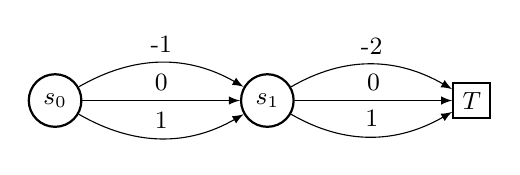
\begin{tikzpicture}[auto,node distance=10mm,>=latex,font=\small]
    \tikzstyle{round}=[thick,draw=black,circle]

    \node[round] (s0) {$s_0$};
    \node[round,right=20mm of s0] (s1) {$s_1$};
    \node[round,rectangle,right=20mm of s1] (T) {$T$};

    \draw[->] (s0) -- node {0} (s1);
    \draw [->] (s0) to [out=30,in=150] node {-1} (s1);
    \draw [->] (s0) to [out=-30,in=210] node {1} (s1);
    \draw[->] (s1) --  node{0}(T);
    \draw [->] (s1) to [out=30,in=150] node{-2} (T);
    \draw [->] (s1) to [out=-30,in=210] node {1} (T);
    % \draw[->] (s0) [out=40,in=100,loop] to coordinate[pos=0.1](aa) (s0);
\end{tikzpicture}
\end{center}
%

Let our initial policy $\piold$ be the equiprobable policy for all states and actions. That is, $\forall\, (s, a)$, $\piold(a \mid s) = \frac{1}{3}$. Consider $\pinew$ to be the following. 
\begin{align*}
    \pinew(\cdot \mid s_0) &= \piold(\cdot \mid s_0)\\
    \pinew(a_0 \mid s_1) &= 3/8 \\
    \pinew(a_1 \mid s_1) &= 2/8\\
    \pinew(a_2 \mid s_1) &= 3/8
\end{align*}
%
Our strategy is the following: show that (1) $\pinew$ reduces the forward KL as it ``commits'' more at $s_1$, but that (2) $\piold$ has higher entropy and thus a higher soft action-value at $s_0$. A straightforward calculation provides the soft value functions of $\piold$ and $\pinew$ at $s_1$.
\begin{align*}
    V_\tau^\piold(s_1) &= -1/3  + \tau \ln 3    \\
    V_\tau^\pinew(s_1) &= -2 \cdot 3/8 + 3/8 + \tau \entropy(\pinew(\cdot \mid s_1)) = -3/8 + \tau\entropy(\pinew(\cdot \mid s_1))
\end{align*}
Recall that the soft action-value can be written as 
\begin{align*}
    Q_\tau^\pi(s, a) := r(s, a) + \gamma \Ex_{s'\sim p(\cdot \mid s, a)}[V^\pi(s)]. 
\end{align*}
Because this MDP is deterministic, we can rewrite the expectation above as the evaluation $V^\pi(s')$. The soft action-value of $\piold$ is 
\begin{align*}
    Q_\tau^\piold(s_0, a_0) &= -1 + \gamma \, V_\tau^\piold(s_1) = \gamma \,\tau \ln 3 - \frac{3 + \gamma}{3}  && Q_\tau^\piold(s_1, a_0) &= -2 \\
    Q_\tau^\piold(s_0, a_1) &= 0 +  \gamma\, V_\tau^\piold(s_1) = \gamma \,\tau\ln3 - \frac{\gamma}{3} && Q_\tau^\piold(s_1, a_1) &= 0 \\
    Q_\tau^\piold(s_0, a_2) &= 1 + \gamma\, V_\tau^\piold(s_1) = \frac{3 - \gamma}{3} + \gamma \,\tau\, \ln3 && Q_\tau^\piold(s_1, a_2) &= 1  
\end{align*}
%
The exponentiated action-value $\boltzmannQ_\tau$ is as follows.
\begin{align*}
    \boltzmannQ_\tau(s, a) := \frac{\exp(Q(s, a) \tau^{-1})}{\sum\limits_b \exp(Q(s, b) \tau^{-1})}
\end{align*}
%
The partition function at $s_1$ is given by the following.
\begin{align*}
    % Z(s_0) &:= \sum_a \exp(Q_\tau^{\piold}(s_0, a) \tau^{-1}) = \exp(\tau^{-1} V^\piold(s_1))(1 + \exp(\tau^{-1}) + \exp(-\tau^{-1})), \\
    Z(s_1) &:= \sum_a \exp(Q_\tau^{\piold}(s_1, a) \tau^{-1}) = 1 + \exp(\tau^{-1}) + \exp(-2\tau^{-1}).
\end{align*}
Calculating the exponentiated soft action-values at $s_1$,
\begin{align*}
    % \boltzmannQ_\tau^\piold(s_0, a_0) &= \frac{\exp(-\tau^{-1} + \tau^{-1}V^\piold(s_1) )}{Z(s_0)} &= \frac{\exp(-\tau^{-1})}{1 + \exp(\tau^{-1}) + \exp(-\tau^{-1})}, \\
    % \boltzmannQ_\tau^\piold(s_0, a_1) &= \frac{\exp(\tau^{-1}V^\piold(s_1) )}{Z(s_0)} &= \frac{1}{1 + \exp(\tau^{-1}) + \exp(-\tau^{-1})}, \\
    % \boltzmannQ_\tau^\piold(s_0, a_2) &= \frac{\exp(\tau^{-1} + \tau^{-1}V^\piold(s_1) )}{Z(s_0)} &= \frac{\exp(\tau^{-1})}{1 + \exp(\tau^{-1}) + \exp(-\tau^{-1})},  \\
    \boltzmannQ_\tau^\piold(s_1, a_0) &= \frac{\exp(-2\tau^{-1})}{1 + \exp(\tau^{-1}) + \exp(-2\tau^{-1})},\\
    \boltzmannQ_\tau^\piold(s_1, a_1) &= \frac{1}{1 + \exp(\tau^{-1}) + \exp(-2\tau^{-1})},\\
    \boltzmannQ_\tau^\piold(s_1, a_2) &= \frac{\exp(\tau^{-1})}{1 + \exp(\tau^{-1}) + \exp(-2\tau^{-1})}.
\end{align*}
The new soft action-value at $s_0$ is given by
\begin{align*}
    Q_\tau^\pinew(s_0, a_0) &= -1 + \gamma \, V^\pinew_\tau(s_1) \\
        &= -1 - \frac{3\gamma}{8} + \gamma\, \tau\, \entropy(\pinew(\cdot \mid s_1)) \\
        &= \frac{-8 - 3 \gamma}{8} + \gamma\, \tau\, \entropy(\pinew(\cdot \mid s_1)),\\
    Q_\tau^\pinew(s_0, a_1) &= - \frac{3\, \gamma }{8} + \gamma\, \tau\,\entropy(\pinew(\cdot \mid s_1)) ,\\
    Q_\tau^\pinew(s_0, a_2) &= \frac{8 - 3\gamma}{8} + \gamma\, \tau\, \entropy(\pinew(\cdot \mid s_1))
\end{align*}

Let's now compare $Q_\tau^\pinew$ and $Q_\tau^\piold$. Note that entropy is maximized by a uniform distribution, so $\tau \,\entropy(\pinew(\cdot \mid s_1)) < \tau \ln 3$, regardless of the value of $\tau > 0$ and $\gamma > 0$. Let's put the reward terms under a common denominator. 
\begin{align*}
    Q^\piold_\tau(s_0, a_0) - Q^\pinew_\tau(s_0, a_0) &> - \frac{3 + \gamma}{3} + \frac{8 + 3 \gamma}{8} &= \frac{\gamma}{24},\\
    Q^\piold_\tau(s_0, a_1) - Q^\pinew_\tau(s_0, a_1) &> - \frac{\gamma}{3} + \frac{3\, \gamma }{8}  &= \frac{\gamma}{24},\\
    Q^\piold_\tau(s_0, a_2) - Q^\pinew_\tau(s_0, a_2) &> \frac{3 - \gamma}{3} - \frac{8 - 3 \gamma}{8} &= \frac{\gamma}{24}.
\end{align*}
% We also have the following. 
% \begin{align*}
%     -11/8 &< -4/3\\
%     -3/8 &< -1/3\\
%     5/8 &< 2/3
% \end{align*}
Thus, for any $\gamma \in (0, 1]$, $Q_\tau^\pinew(s_0, a) < Q_\tau^\piold(s_0, a)$ for all actions $a$. 

% Let's now set $\tau = 1$. 
Let's now compare the forward KL divergences. Because the policies are the same at $s_0$, we have 
\begin{align*}
    \KL(\boltzmannQ_\tau^\piold(s_0, \cdot) \parallel \pinew(\cdot \mid s_0)) &= \KL(\boltzmannQ_\tau^\piold(s_0, \cdot) \parallel \piold(\cdot \mid s_0)).
\end{align*}
Calculating the rest of the forward KL divergences,
\begin{align*}
    % \KL(\boltzmannQ_\tau^\piold(s_0, \cdot) \parallel \piold(\cdot \mid s_0)) &= -\entropy(\boltzmannQ_\tau^\piold(s_0, \cdot)) - \frac{1}{Z(s_1)} (\exp(-1) \log(1/3) + \log(1/3) + \exp(1) \log(1/3))  \\
    &\KL(\boltzmannQ_\tau^\piold(s_1, \cdot) \parallel \piold(\cdot \mid s_1)) =\\
    &\quad-\entropy(\boltzmannQ_\tau^\piold(s_1, \cdot)) - \log(1/3) \frac{\exp(-2\tau^{-1}) + 1 + \exp(\tau^{-1})}{1 + \exp(\tau^{-1}) + \exp(-2\tau^{-1})}   \\
    &\KL(\boltzmannQ_\tau^\piold(s_1, \cdot) \parallel \pinew(\cdot \mid s_1)) =\\
    &\quad-\entropy(\boltzmannQ_\tau^\piold(s_1, \cdot)) - \frac{\exp(-2\tau^{-1}) \log(3/8)+ \log(2/8) + \exp(\tau^{-1}) \log(3/8)}{1 + \exp(\tau^{-1}) + \exp(-2\tau^{-1})}   
\end{align*}
In order to have $\KL(\boltzmannQ_\tau^\piold(s_1, \cdot) \parallel \piold(\cdot \mid s_1)) > \KL(\boltzmannQ_\tau^\piold(s_1, \cdot) \parallel \pinew(\cdot \mid s_1))$, it is sufficient and necessary to have
\begin{align*}
    &- \log(1/3) \frac{\exp(-2\tau^{-1}) + 1 + \exp(\tau^{-1})}{1 + \exp(\tau^{-1}) + \exp(-2\tau^{-1})} \\
    &\quad > - \frac{\exp(-2\tau^{-1}) \log(3/8)+ \log(2/8) + \exp(\tau^{-1}) \log(3/8)}{1 + \exp(\tau^{-1}) + \exp(-2\tau^{-1})}.
\end{align*}
Or, after simplifying,
\begin{align*}
    &- \log(1/3) (\exp(-2\tau^{-1}) + 1 + \exp(\tau^{-1})) \\ 
    &\quad > - (\exp(-2\tau^{-1}) \log(3/8)+ \log(2/8) + \exp(\tau^{-1}) \log(3/8))\\
    &\iff \exp(-2\tau^{-1})(\log(3/8) - \log(1/3)) + \log(2/8) - \log(1/3)\\
    &\quad\quad+ \exp(\tau^{-1})(\log(3/8) - \log(1/3)) > 0\\
    &\iff \exp(-2\tau^{-1})\log(9/8) + \log(3/4) + \exp(\tau^{-1})\log(9/8) > 0\\
    &\iff \log(9/8) + \log(3/4)\exp(2 \tau^{-1}) + \exp(3\tau^{-1})\log(9/8) > 0.
\end{align*}
Setting $y = \exp(\tau^{-1})$, we are interested in the cubic inequality
\begin{align*}
    \log(9/8) + \log(3/4) y^2 + y^3\log(9/8) > 0.
\end{align*}
Noting that the leading term of the cubic is positive, there must be some $y_0$ such that for $y > y_0$, the inequality above holds. This $y_0$ must be the largest root of the cubic expression. A root-solver gives $y_0 > 2.25$, so the above inequality holds for $\exp(\tau^{-1}) = y > 2.25$, or in other words for $1.23 \approx \frac{1}{\log 2.25} > \tau$.

\end{proof}
%
\Cref{lem:forward-kl-counterexample} shows that there is an MDP and two policies in which one policy $\pinew$ can have a lower FKL, but fail to be a better policy for small enough $\tau$. It might seem like \Cref{lem:forward-kl-counterexample} could contradict the RKL improvement result in \Cref{lem:stronger-sac}, but \Cref{lem:forward-kl-counterexample} is a statement about a particular policy, and not about any policy that reduces the RKL.

From examining the proof of \Cref{lem:forward-kl-counterexample}, it might also be surprising that the result holds for sufficiently small $\tau$. That is, for $\tau < \tau_0$, for some $\tau_0$, there will always be a policy that reduces the FKL, but that has strictly worse performance than the previous policy. Such a result might seem unintuitive since one would expect that the more one reduces the FKL, the better the policy should be, given that the FKL is minimized by setting the subsequent policy to be exactly the target distribution. Nevertheless, such reasoning says nothing about the path of policies to the superior, target distribution policy. 

A natural question is if this counterexample is pathological. Since reducing the FKL to 0 corresponds to reducing the RKL to 0 (i.e., setting $\pinew = \boltzmannQ^\piold_\tau$), it seems plausible that if the FKL is reduced enough, the new policy $\pinew$ will be better. One may also wonder if by selecting a temperature judiciously enough, optimizing for the forward KL might induce policy improvement. With some qualifications, the answer is in the positive. 
%
\begin{proposition}[Policy Improvement for FKL with Sufficient Reduction]\label{prop:forward-kl-surrogate-2}
Assume a discrete action space with $|\actionspace| < \infty$, with a policy space $\Pi$ that consists of policies where $\pi(a \mid s) > 0$ for all $a$. Let $C$, $\piold, \pinew \in \Pi$ be such that for a state $s$,
\begin{align}\label{eq:forward-improvement}
    \KL(\boltzmannQ^{\piold}(s, \cdot) \parallel \pinew (\cdot \mid s)) + C \leq \KL(\boltzmannQ^{\piold}(s, \cdot) \parallel \piold(\cdot \mid s)),
\end{align}
where $C$ additionally satisfies
\begin{align*}
    C &\geq  \frac{1}{2}\sum_a  \left(1 - \frac{1}{\piold(a \mid s)}\right)^2 \left(1 + \frac{Q^\piold(s, a)}{\tau} + \frac{\exp(\tau^{-1} Q^\piold(s, a)) Q^\piold(s, a)^2}{2\tau^2}\right) \\
    &\quad + \frac{1}{2} \sum_a \exp(\tau^{-1} Q^\piold(s, a)) \tau^{-2} Q^\piold(s, a)^2 (1 - \piold(a \mid s))
\end{align*}
with $\tau > 0$. Then,
\begin{align*}
    \sum_a Q^{\piold}(s, a) \piold(a \mid s) \leq \sum_a Q^{\piold}(s, a) \pinew(a \mid s). 
\end{align*}
\end{proposition}
\begin{proof}

For the steps below, we will need to consider shifted, positive values $Q^{\piold}(s, a) + b $ where $b \defeq \max(0, -\min_{a \in \actionspace} Q^{\piold}(s,a)) + 0.01$. This shift does not affect \Cref{eq:forward-improvement} because the Boltzmann function is invariant to shifts in the logits. 
It suffices to focus on a single state $s$. We will suppress dependence on this state for notational simplicity. Let $\pi(a) \defeq \piold(a | s)$ and $Q(a) \defeq Q^{\piold}(s, a) + b > 0$. After cancelling the common entropy term and multiplying both sides by the partition function, \Cref{eq:forward-improvement} yields
\begin{align}\label{eq:first-ineq}
    \sum_a \exp(\tau^{-1} Q(a)) \log \frac{1}{\pinew(a)} + C \leq \sum_a \exp(\tau^{-1} Q(a)) \log \frac{1}{\piold(a)}.
\end{align}
For $x \geq 0$, we have $1 + x \leq \exp(x)$ and for $x \in (0, 1)$ we have $ \log \frac{1}{x} = -\log(x) \geq 1 - x$. Since we assumed $Q(a) > 0$ and $\piold$, $\pinew$ are not deterministic, these inequalities may be applied. Applying them to \Cref{eq:first-ineq} gives
\begin{align}\label{eq:second-ineq}
    \sum_a (1 + \tau^{-1} Q(a)) (1 - \pinew(a)) + C \leq \sum_a \exp(\tau^{-1} Q(a)) \log\frac{1}{\piold(a)}.
\end{align}
To get any further, we proceed by Taylor expansion. We will expand $\exp(x)$ around $x = 0$ and $\log (x)$ around $x = 1$. Now, using the Lagrange form of the remainder of Taylor expansions yields
\begin{align*}
    \exp(\tau^{-1} Q(a)) &= 1 + \tau^{-1} Q(a) + \frac{1}{2}\exp(\xi_a) \tau^{-2} Q(a)^2,\\
    \implies \exp(\tau^{-1} Q(a)) &\leq 1 + \tau^{-1} Q(a) + \frac{1}{2}\exp(\tau^{-1} Q(a)) \tau^{-2} Q(a)^2,\\
    \log(\piold(a)) &= \piold(a) - 1 - \frac{1}{2\kappa_a^2} (\piold(a) - 1)^2,\\
    \implies \log \frac{1}{\piold(a)} &= 1 - \piold(a) + \frac{1}{2\kappa_a^2} (\piold(a) - 1)^2\\
    \implies \log \frac{1}{\piold(a)} &\leq 1 - \piold(a) + \frac{1}{2\piold(a)^2} (\piold(a) - 1)^2\\
    \implies \log \frac{1}{\piold(a)} &\leq 1 - \piold(a) + \frac{1}{2} \left(1 - \frac{1}{\piold(a)}\right)^2
\end{align*}
for some $\xi_a \in (0, \tau^{-1}Q(a))$ and $\kappa_a \in (\piold(a), 1)$. 
Using the inequalities on the RHS of \Cref{eq:second-ineq} yields the following. 
\begin{align*}
    &\sum_a \exp(\tau^{-1} Q(a)) \log\frac{1}{\piold(a)}\\
    &\hspace{2em} \leq \sum_a (1 + \tau^{-1} Q(a))(1 - \piold(a)) + \mathbf{X},
\end{align*}
where $\mathbf{X}$ represents terms we have neglected for the moment. From re-examining \Cref{eq:second-ineq}, noting that $\sum_a (1 - \piold(a)) = \sum_a (1 - \pinew(a))$, and canceling out $\sum_a \tau^{-1} Q(a)$ on both sides, we have
\begin{align*}
    -\sum_a \tau^{-1}Q(a) \pinew(a) + C &\leq -\sum_a \tau^{-1}Q(a) \piold(a) + \mathbf{X}\\
    C -\mathbf{X} &\leq \tau^{-1} \sum_a Q(\pinew(a) - \piold(a))
\end{align*}

Notice that 
\begin{align*}
\sum_a Q(a)\pinew(a) &= \sum_a (Q^{\piold}(s, a) + b )\pinew(a) \\
&=  \sum_a Q^{\piold}(s, a) \pinew(a) +  b \sum_a \pinew(a) \\
&= \sum_a Q^{\piold}(s, a) \pinew(a) +  b \\
\implies  \sum_a Q(a)(\pinew(a) - \piold(a)) &=  \sum_a Q^{\piold}(s,a)(\pinew(a) - \piold(a))
\end{align*}
%
Therefore, to show that $\sum_a Q^{\piold}(s,a)\pinew(a) \ge \sum_a Q^{\piold}(s,a)\piold(a)$, it suffices that $C -\mathbf{X} \geq 0$, or equivalently that $C \geq \mathbf{X}$. 
\begin{align*}
    \mathbf{X} &:=  \frac{1}{2}\sum_a  \left(1 - \frac{1}{\piold(a)}\right)^2 (1 + \tau^{-1} Q(a) + \frac{1}{2}\exp(\tau^{-1} Q(a)) \tau^{-2} Q(a)^2) \\
    &\quad + \frac{1}{2} \sum_a \exp(\tau^{-1} Q(a)) \tau^{-2} Q(a)^2 (1 - \piold(a))
\end{align*}
Noting that every term is non-negative by assumption, the conclusion follows.
\end{proof}
The conclusions of \Cref{prop:forward-kl-surrogate-2} hold if $C$ is large enough; as $\tau$ decreases, $C$ must be larger, which explain the failure of policy improvement in \Cref{lem:forward-kl-counterexample}. On the other hand, if $\tau$ is large, then the requirement for $C$ becomes less onerous, although the resulting conclusion might be quite weak; soft action-values for large $\tau$ become dominated by the entropy term, weighing much less the contribution of reward from the environment. 

How large can the minimal $C$ required get? Using the MDP of \Cref{lem:forward-kl-counterexample}, in \Cref{fig:prop3-c} we plot the minimal $C$ as a function of temperature. The minimal $C$ is in fact larger than $\KL(\boltzmannQ^\piold(s_1, \cdot) \parallel \piold(\cdot \mid s_1))$! This suggests that the minimal $C$ is in fact an overestimate, which seems due to the looseness of the bounds, $\log x \leq x - 1$ in particular, we used in deriving it. 
\begin{figure}[!htb]
    \centering
    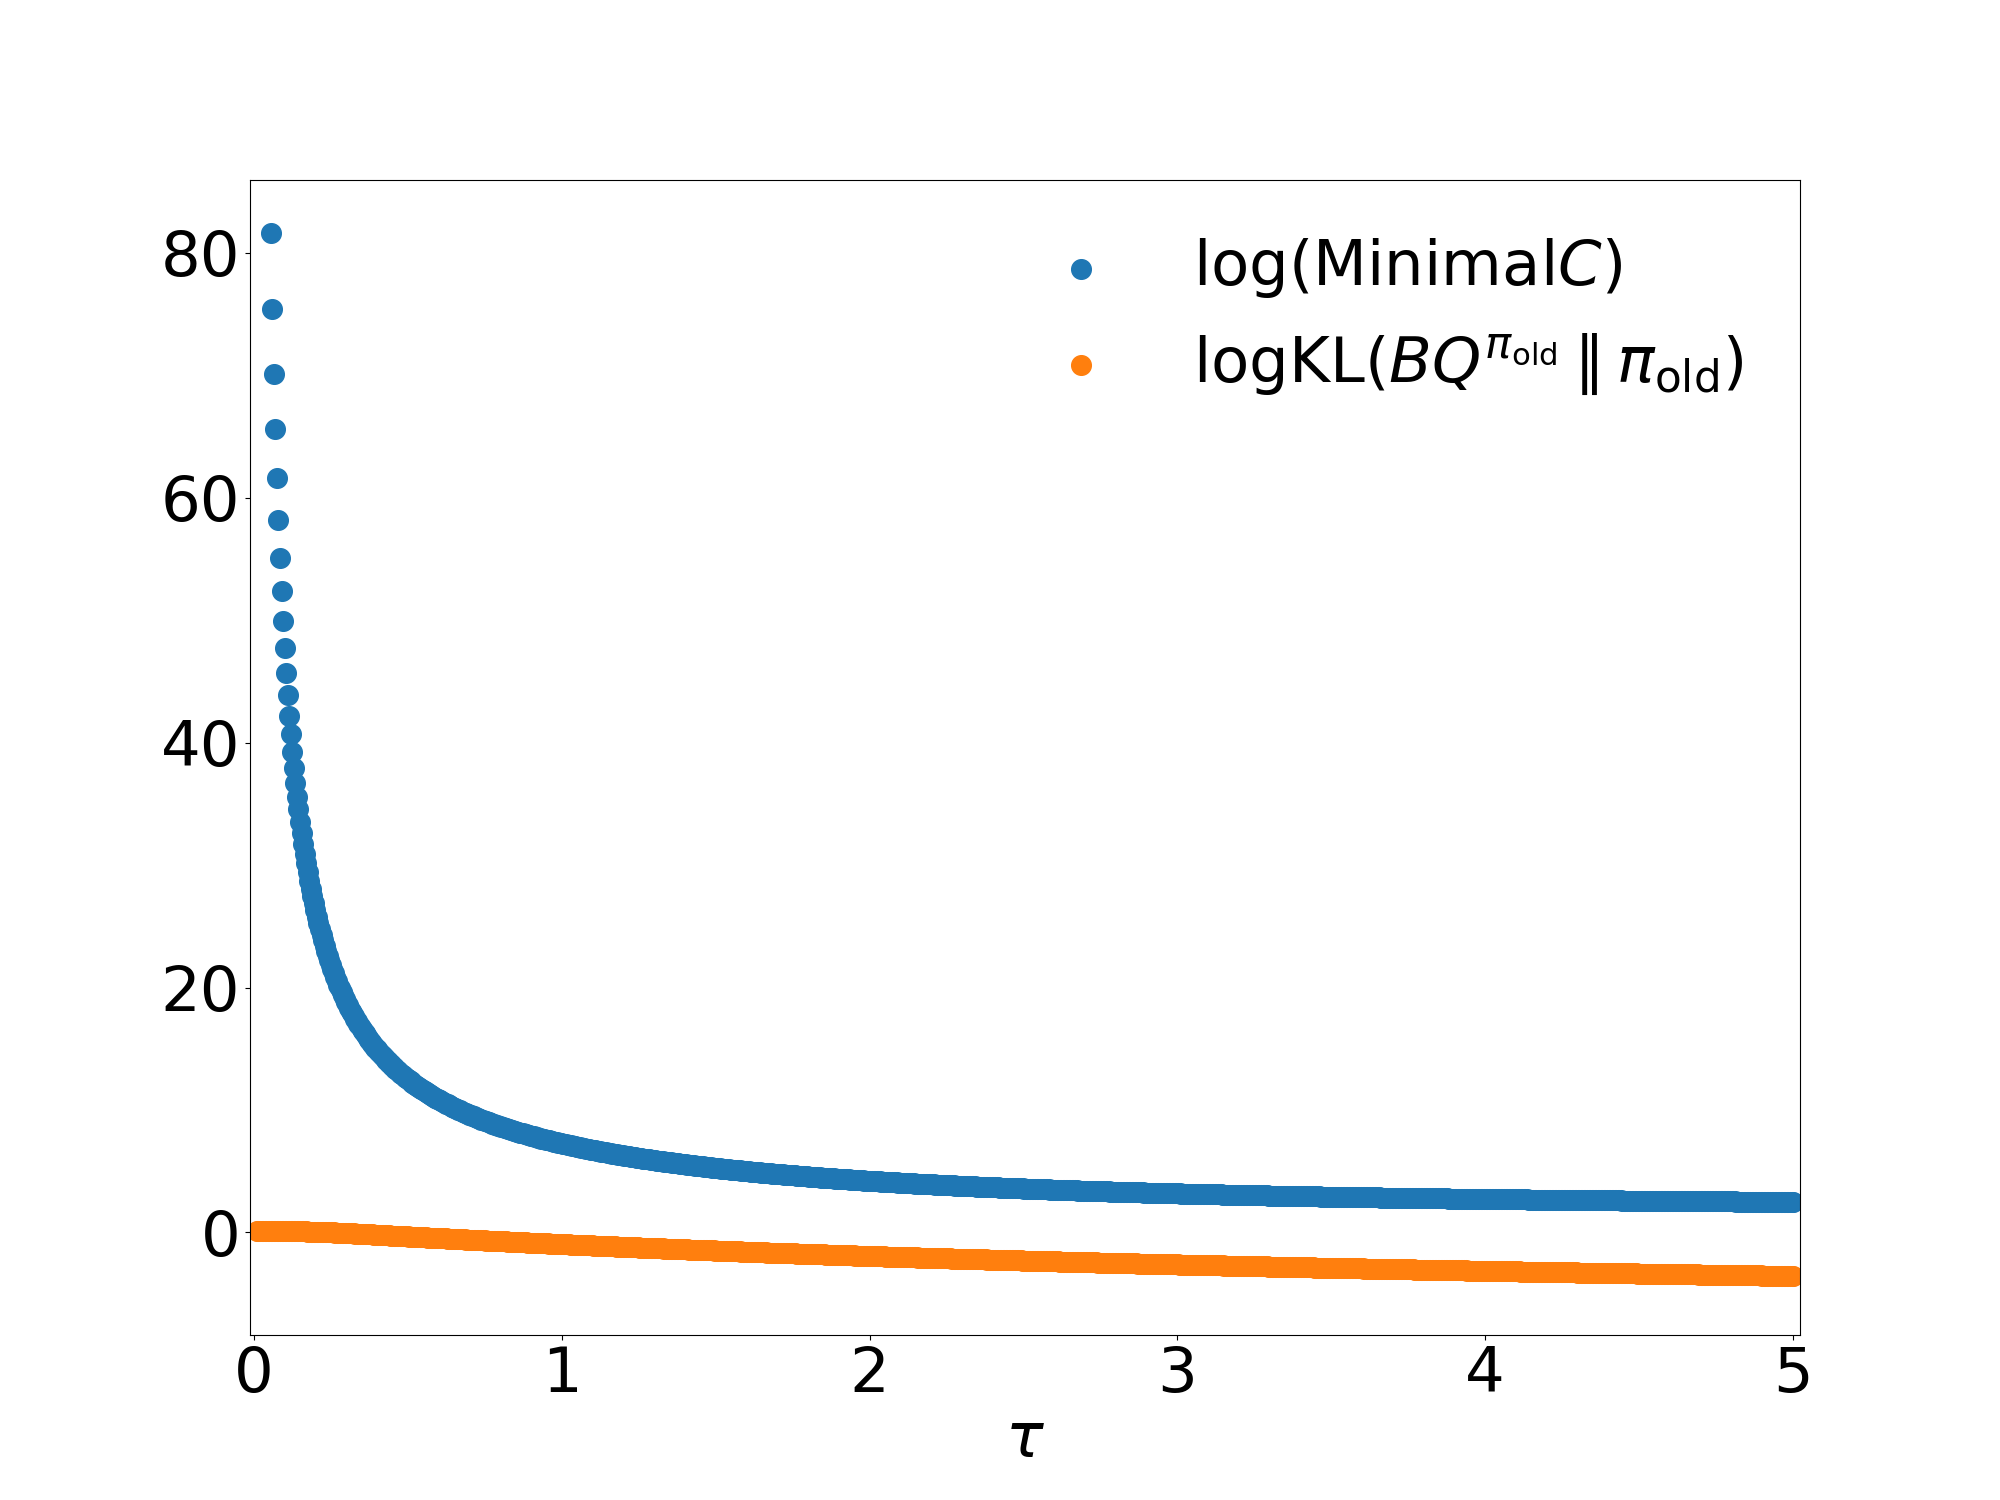
\includegraphics[width=\linewidth]{figs/theory/prop3.png}
    \caption{The minimal $C$ in \Cref{prop:forward-kl-surrogate-2} as a function of $\tau$, plotted against the KL divergence between $\boltzmannQ^\piold$ and $\piold$ at $s_1$ of the MDP in \Cref{lem:forward-kl-counterexample}.}
    \label{fig:prop3-c}
\end{figure}

If the conclusions of \Cref{fig:prop3-c} do hold across all states, and with an additional assumption, we can guarantee policy improvement. 
\begin{corollary}\label{cor:fkl-pi}
If 
\begin{align*}
    \Ex_{d^\pinew, \piold}[ Q^\piold_\tau(s, a)]\leq \Ex_{d^\pinew, \pinew}[Q^\piold_\tau(s, a)],
\end{align*}
and if 
\begin{align*}
    \tau \Ex_{d^\pinew}[\entropy(\pinew(\cdot \mid s))] \geq \tau \Ex_{d^\pinew}[\entropy(\piold(\cdot \mid s))],
\end{align*}
then $\eta_\tau(\pinew) \geq \eta_\tau(\piold)$. This conclusion also holds for $\tau = 0$.
\end{corollary}
\begin{proof}
If $\tau = 0$, then $\sum_a \piold(a \mid s) Q^{\piold}(s, a) = V^{\piold}(s)$. If the above holds for all states $s$, then $V^{\piold}(s) \leq \sum_a Q^{\piold}(s, a) \pinew(a \mid s)$ for all states and so $V^{\pinew} \geq V^{\piold}$ by the classical policy improvement theorem \citep{sutton2018reinforcement}. It follows that $\eta(\pinew) \geq \eta(\piold)$.

If $\tau > 0$, we may use \Cref{lemma:soft-performance-difference}, the soft performance difference lemma. Note that since we are working with soft value functions, we have the following relation between the soft state-value and the soft action-value. 
\begin{align*}
    \sum_a Q_\tau^\piold(s, a) \piold(a \mid s) = V_\tau^\piold(s) - \tau \entropy(\piold(\cdot \mid s)).
\end{align*}
Using the first assumption of the Corollary,
\begin{align*}
    \Ex_{d^\pinew, \piold}[V_\tau^\piold(s) + \tau \log\piold(\cdot \mid s)] &= \Ex_{d^\pinew, \piold}[ Q_\tau^\piold(s, a)] \\
    &\leq \Ex_{d^\pinew, \pinew}[ Q_\tau^\piold(s, a)].
\end{align*}
Rearranging and taking expectations, we have
\begin{align*}
    \Ex_{d^\pinew, \pinew}[Q_\tau^\piold(s, a) -& V_\tau^\piold(s)] \geq \tau \Ex_{d^\pinew, \piold}[\log \piold(\cdot \mid s)],\\
    \Ex_{d^\pinew, \pinew}[A_\tau^\piold(s, a)] &\geq \tau \Ex_{d^\pinew}[\Ex_{\piold}[\log \piold(\cdot \mid s)] - \Ex_{\pinew}[\log \piold(\cdot \mid s)]].\\
    &\quad \triangleright \text{adding } -\tau \Ex_{d^\pinew, \pinew}[\log \piold(\cdot \mid s)] \text{ to both sides}
\end{align*}
From Gibbs's inequality, the entropy of any distribution is strictly less than the cross-entropy of that distribution with any other distribution. In other words,
\begin{align*}
    \entropy(\pinew(\cdot \mid s)) &\leq \entropy(\pinew(\cdot \mid s), \piold(\cdot \mid s))\\
    -\Ex_\pinew[\log \pinew(\cdot \mid s)] &\leq - \Ex_\pinew[\log \piold(\cdot \mid s))]
\end{align*}
Applying this inequality,
\begin{align*}
    \Ex_{d^\pinew, \pinew}[A_\tau^\piold(s, a)] &\geq \tau \Ex_{d^\pinew}[\Ex_{\piold}[\log \piold(\cdot \mid s)] - \Ex_{\pinew}[\log \pinew(\cdot \mid s)]]\\
    &= \tau \Ex_{d^\pinew}[ \entropy (\pinew(\cdot \mid s)) - \entropy(\piold(\cdot \mid s))]\\
    &\geq 0\\
    &\quad \triangleright \text{by the entropy assumption of the Corollary}
\end{align*}
\end{proof}

\noindent The entropy assumption in \Cref{cor:fkl-pi} is a bit strange; for $\pinew$ to be better, it must ``commit'' less to actions, the opposite of what we would expect a policy to do when learning optimal actions. 

\subsection{Summary}
Here are some takeaways of the above discussion. 
\begin{enumerate}
    \item The RKL has a stronger policy improvement result than the FKL as it requires only that the RKL of $\pinew$ be no greater than the RKL of $\piold$.
    \item The FKL can fail to induce policy improvement, but this failure is linked to a temperature that is too low and/or an insufficient reduction in the FKL. For a large enough reduction and large enough temperature, coupled with an additional entropy assumption, policy improvement follows. 
\end{enumerate}


There are some limitations of this theory. We had to assume a finite action space for \Cref{prop:forward-kl-surrogate-2}. The reason here was to ensure that we could sensibly manipulate the remainder terms in the Taylor expansions. A general treatment of action spaces would at least require some work into the measurability and integrability of such terms as a function of the action. Moreover, the theory developed in this chapter is under ideal settings, assuming in particular access to the true value functions. For \Cref{prop:forward-kl-surrogate-2,cor:fkl-pi}, the looseness of the bounds we employed resulted in extremely strong sufficient conditions for FKL policy improvement. As we will see in our experiments, the FKL is often able to induce policy improvement in practice, suggesting a gap between the theory developed and the practical performance. 

%------------------------------------------------------------------------------------------------------------------------------
\section{Optimization Behavior in Microworlds} 
The goal in this section is to understand differences between FKL and RKL in terms of (1) the loss surface and (2) the behaviour of iterates optimized under the losses. By behaviour, we mean whether the iterates reach multiple local optima, how stable iterates under that loss are, and how often iterates reach the global optimum (or optima). Given the fine-grained nature of our questions, we focus upon small-scale environments, which we call \textit{microworlds}. Doing so allows us to avoid any possible confounding factors associated with larger, more complicated environments, and furthermore allows us more fully to separate any issues to do with stochasticity. 

We begin with continuous actions, and note results for discrete actions in \Cref{sec:microworld-discrete-actions}. We use two types of low-dimensional microworlds to allow us to visualize and thoroughly investigate behavior.

Our first microworld is a \textbf{Bimodal Bandit} in \Cref{fig:bimodal-bandit}. For continuous actions, we designed a continuous bandit with action space $[-1, 1]$ and reward function $Q(a) := \exp( -\tfrac{1}{2} (\tfrac{2 a + 1}{0.2})^2 ) + \tfrac{3}{2} \exp(-\tfrac{1}{2} (\tfrac{2 a - 1}{0.2})^2)$. The two unequal modes at -0.5 and 0.5 enable us to test the mean-seeking and mode-seeking behavior as well as simulate a realistic scenario where the agent's policy parameterization (here, unimodal) cannot represent the true distribution (bimodal). For discrete actions, we designed a discrete bandit with rewards $(1, 1.5)$. 

Our second microworld is the \textbf{Switch-Stay} domain in \Cref{fig:switch-stay}. From $s_0$, action $0$ (stay) gives a reward of 1 and transitions to state $0$. From $s_1$, action 0 gives a reward of 2 and transitions to $s_1$. From $s_0$, action 1 (switch) gives a reward of -1 and transitions to $s_1$, while action 1 from $s_1$ gives a reward of 0 and transitions to $s_0$. 

To adapt this environment to the continuous action setting, we treat actions $> 0$ as switch and actions $\leq 0$ as stay.  We set $\gamma = 0.9$ to ensure that the optimal action from $s_0$ is to switch, which ensures the existence of a short-term/long-term trade-off inherent to realistic RL environments. 

\begin{figure}[!htb]
    \centering
    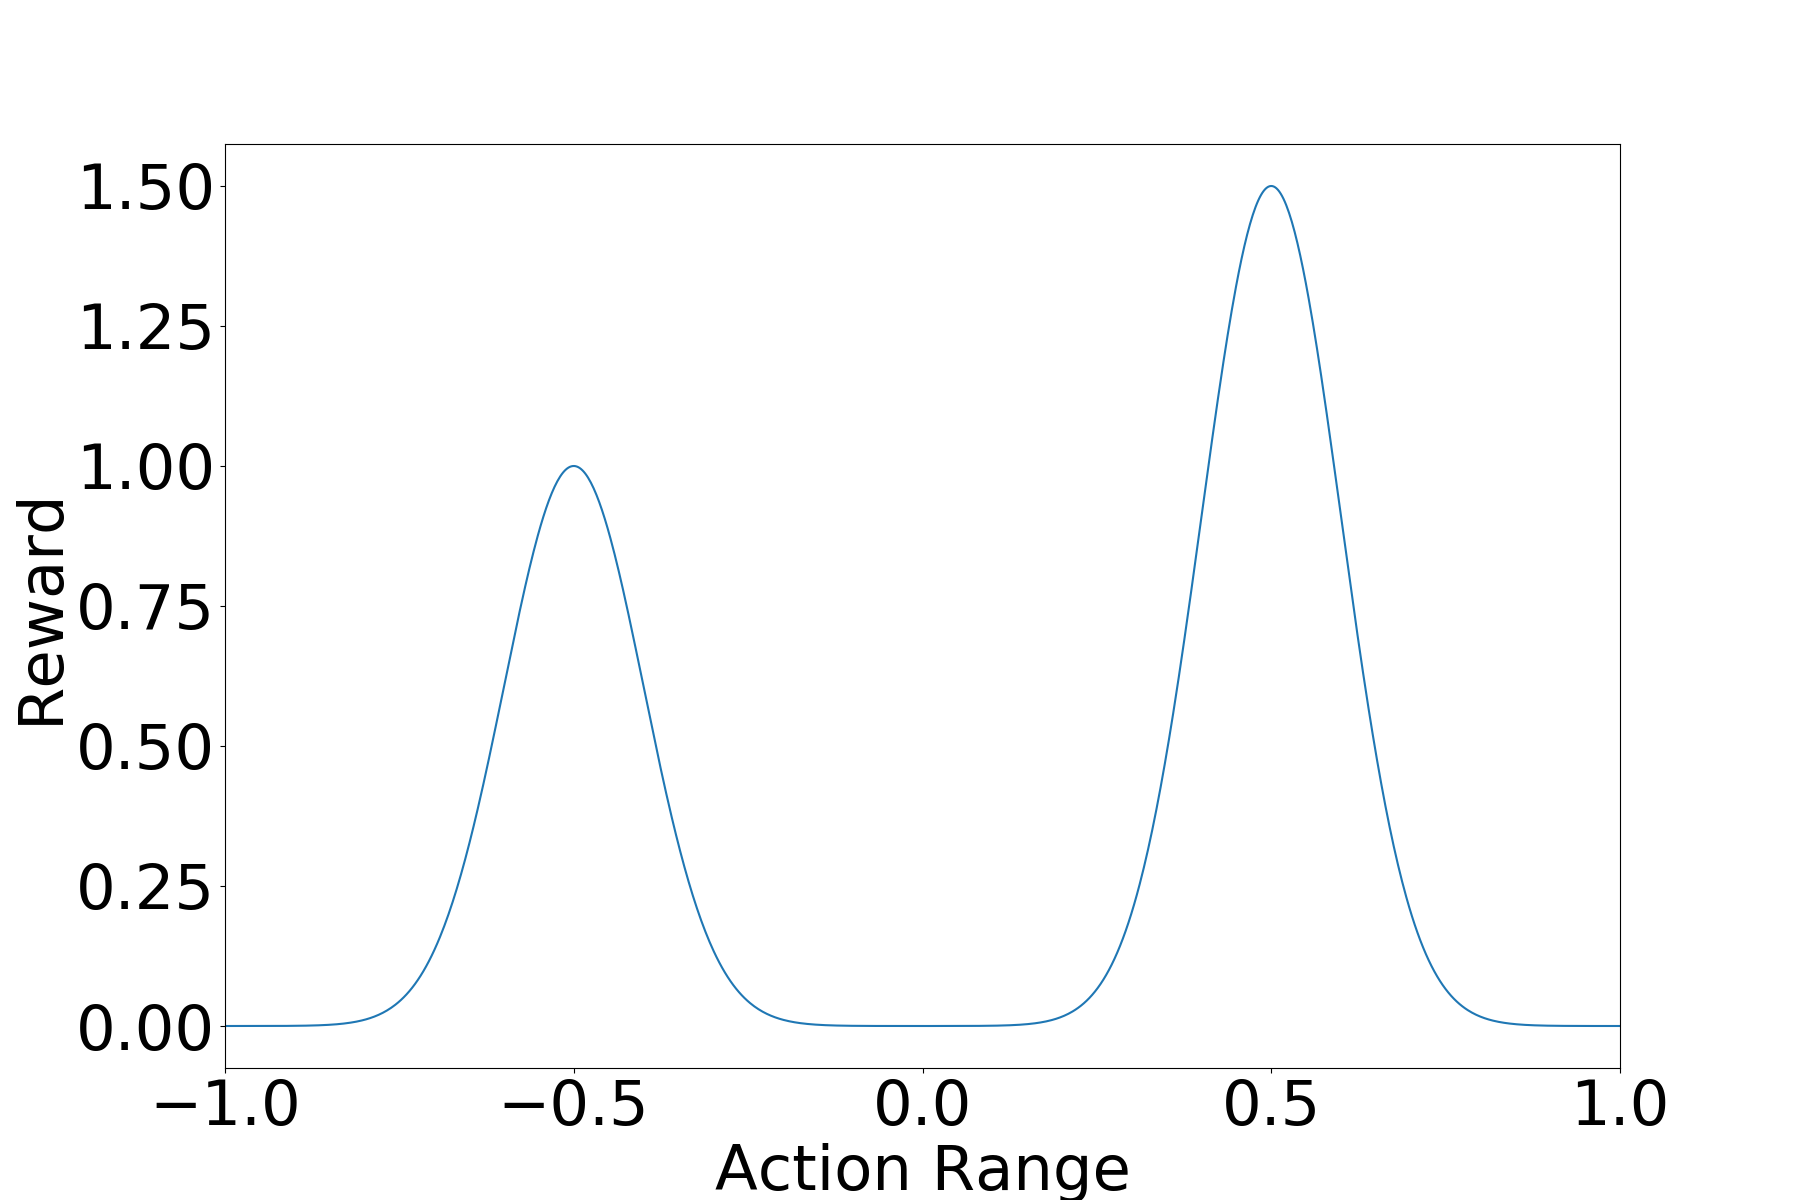
\includegraphics[width=0.5\linewidth]{figs/bandit/bimodal-bandit.png}
    \caption{Continuous-action Bimodal Bandit.}
    \label{fig:bimodal-bandit}
\end{figure}


\begin{figure}[!htb]
  \hspace*{10em}\resizebox{0.4\columnwidth}{!}{%
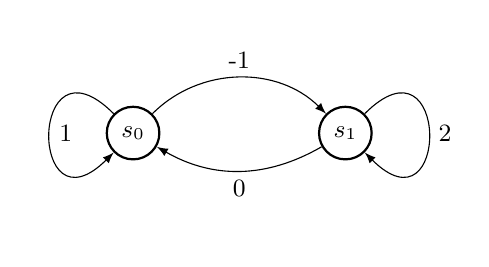
\begin{tikzpicture}[auto,node distance=10mm,>=latex,font=\small]
    \tikzstyle{round}=[thick,draw=black,circle]

    \node[round] (s0) {$s_0$};
    \node[round,right=20mm of s0] (s1) {$s_1$};

    \draw[->] (s0) to [out=45, in=135] node {-1} (s1);
    \draw [->] (s0) to [out=135,in=225, loop] node {1} (s0);
    \draw [->] (s1) to [out=210,in=330] node{0} (s0);
    \draw [->] (s1) to [out=45,in=-45, loop] node {2} (s1);
\end{tikzpicture}}
    \caption{Switch-Stay.}
    \label{fig:switch-stay}
\end{figure}%

\subsection{Implementation Details}
\noindent All policies are tabular in the state. To calculate the FKL and RKL for the continuous action setting, we use the Clenshaw-Curtis \citep{clenshaw1960method} numerical integration scheme with 1024 points from the package quadpy \citep{schlomerquadpy}, excluding the first and the last points at -1 and 1 because of numerical stability. Numerical integration is used to minimize any confounding influence of stochasticity on the behaviour, but we also note additional results for Monte Carlo integration in \Cref{sec:stochastic-microworld}.

To calculate the Hard FKL, we use the true maximum action as determined by the environment. In the discrete action setting, we may calculate the non-hard FKL losses in closed form by summing across all actions. For Switch-Stay, we calculate and optimize the mean KL across the two states.

We use the true action-values when calculating the KL losses; in the bimodal bandit, the action-value is given by the reward function, while in Switch-Stay it is calculated (i.e., not learned). For policy parameterizations, in continuous action settings we use a Gaussian policy with mean and variance learned as $(\hat{\mu}, \log(1+\exp(\hat{\sigma}))$ and in discrete action settings we use a softmax policy. The action sampled from the learned Gaussian is passed through $\tanh$ to ensure that the action is in the feasible range $[-1, 1]$ and to avoid the bias induced in the policy gradient when action ranges are not enforced \citep{chou2017improving}. 

Finally, we use the RMSprop optimizer \citep{tieleman2012lecture}. Overall trends for Adam \citep{kingma2014adam} were similar to those for RMSprop, while results for SGD resulted in slower learning for both FKL and RKL and a wider range of limit points, most likely due to oscillation from the constant step-size. We focus on RMSprop here to avoid any confounding factors associated with momentum. 


\subsection{Continuous Action Results in the Bimodal Bandit}
Firstly, we might expect the FKL to have a smoother loss surface. Given that policies often are part of an exponential class (e.g., softmax policy), having the policy $\pi$ be the second argument of $\KL(p \parallel q)$ might be advantageous as $\KL(p \mid \pi)$ removes the exponential in $\pi$. 

\subsubsection{Loss Surface}
% \myparagraph{Optimization Surface for the Bimodal Bandit}
We visualize the KL loss surfaces in \Cref{fig:bandit-heatmap} with five different temperatures. The heatmaps depict the loss for each mean and standard deviation pair. The last row depicts the target distribution over which the KL loss is optimized. The surfaces suggest the following. 

\textbf{1)} The FKL surface has a single valley, while the RKL surface has two valleys that are separated from one another. In this sense, the FKL surface seems much smoother than the RKL surface, suggesting that iterates under the FKL will more likely reach the global optimum than iterates under the RKL, which seem likely to fall into either of the valleys. 

\textbf{2)} The smoothness of the RKL landscape increases with temperature as the gap between the peaks becomes less steep. A higher temperature also causes the valley in the FKL map to become less sharply peaked, and for the optimal $\mu$ to move closer to 0. The optimal $\mu$ for the FKL seems to move more quickly to zero, as $\tau$ increases, than the optimal $\mu$ for the RKL, although both eventually reach 0. It is possible that the FKL may become suboptimal sooner than the RKL as $\tau$ increases. 

\textbf{3)} It may seem strange that two valleys exist for the RKL at $\tau = 0$ given that the target distribution is unimodal. Note, however, that when $\tau = 0$, the loss function is no longer a distributional loss; that is, we are no longer minimizing any pseudo-distance between the policy and a distribution. 


% \textbf{3)} As the temperature decreases, the target distribution becomes unimodal; making the mean and the mode become identical; the global optimum for both the FKL and RKL is at the optimal peak.

% We also considered the effects of numerical integration and the $\tanh$ transformation.
% \textbf{6)} FKL seems to be more robust to numerical integration error. When reducing the number of integration points, there was no visible difference in the FKL loss surface but wavelet patterns are observed in the RKL loss surface (Appendix H).
% \textbf{7)} The optimization surface for a Gaussian policy without the $\tanh$ transformation is shown in Appendix H. In this setting, suboptima appear along the edges in all soft RKL surfaces, while FKL loss surface seems unaffected.

\begin{figure}[!htb]
    \centering
    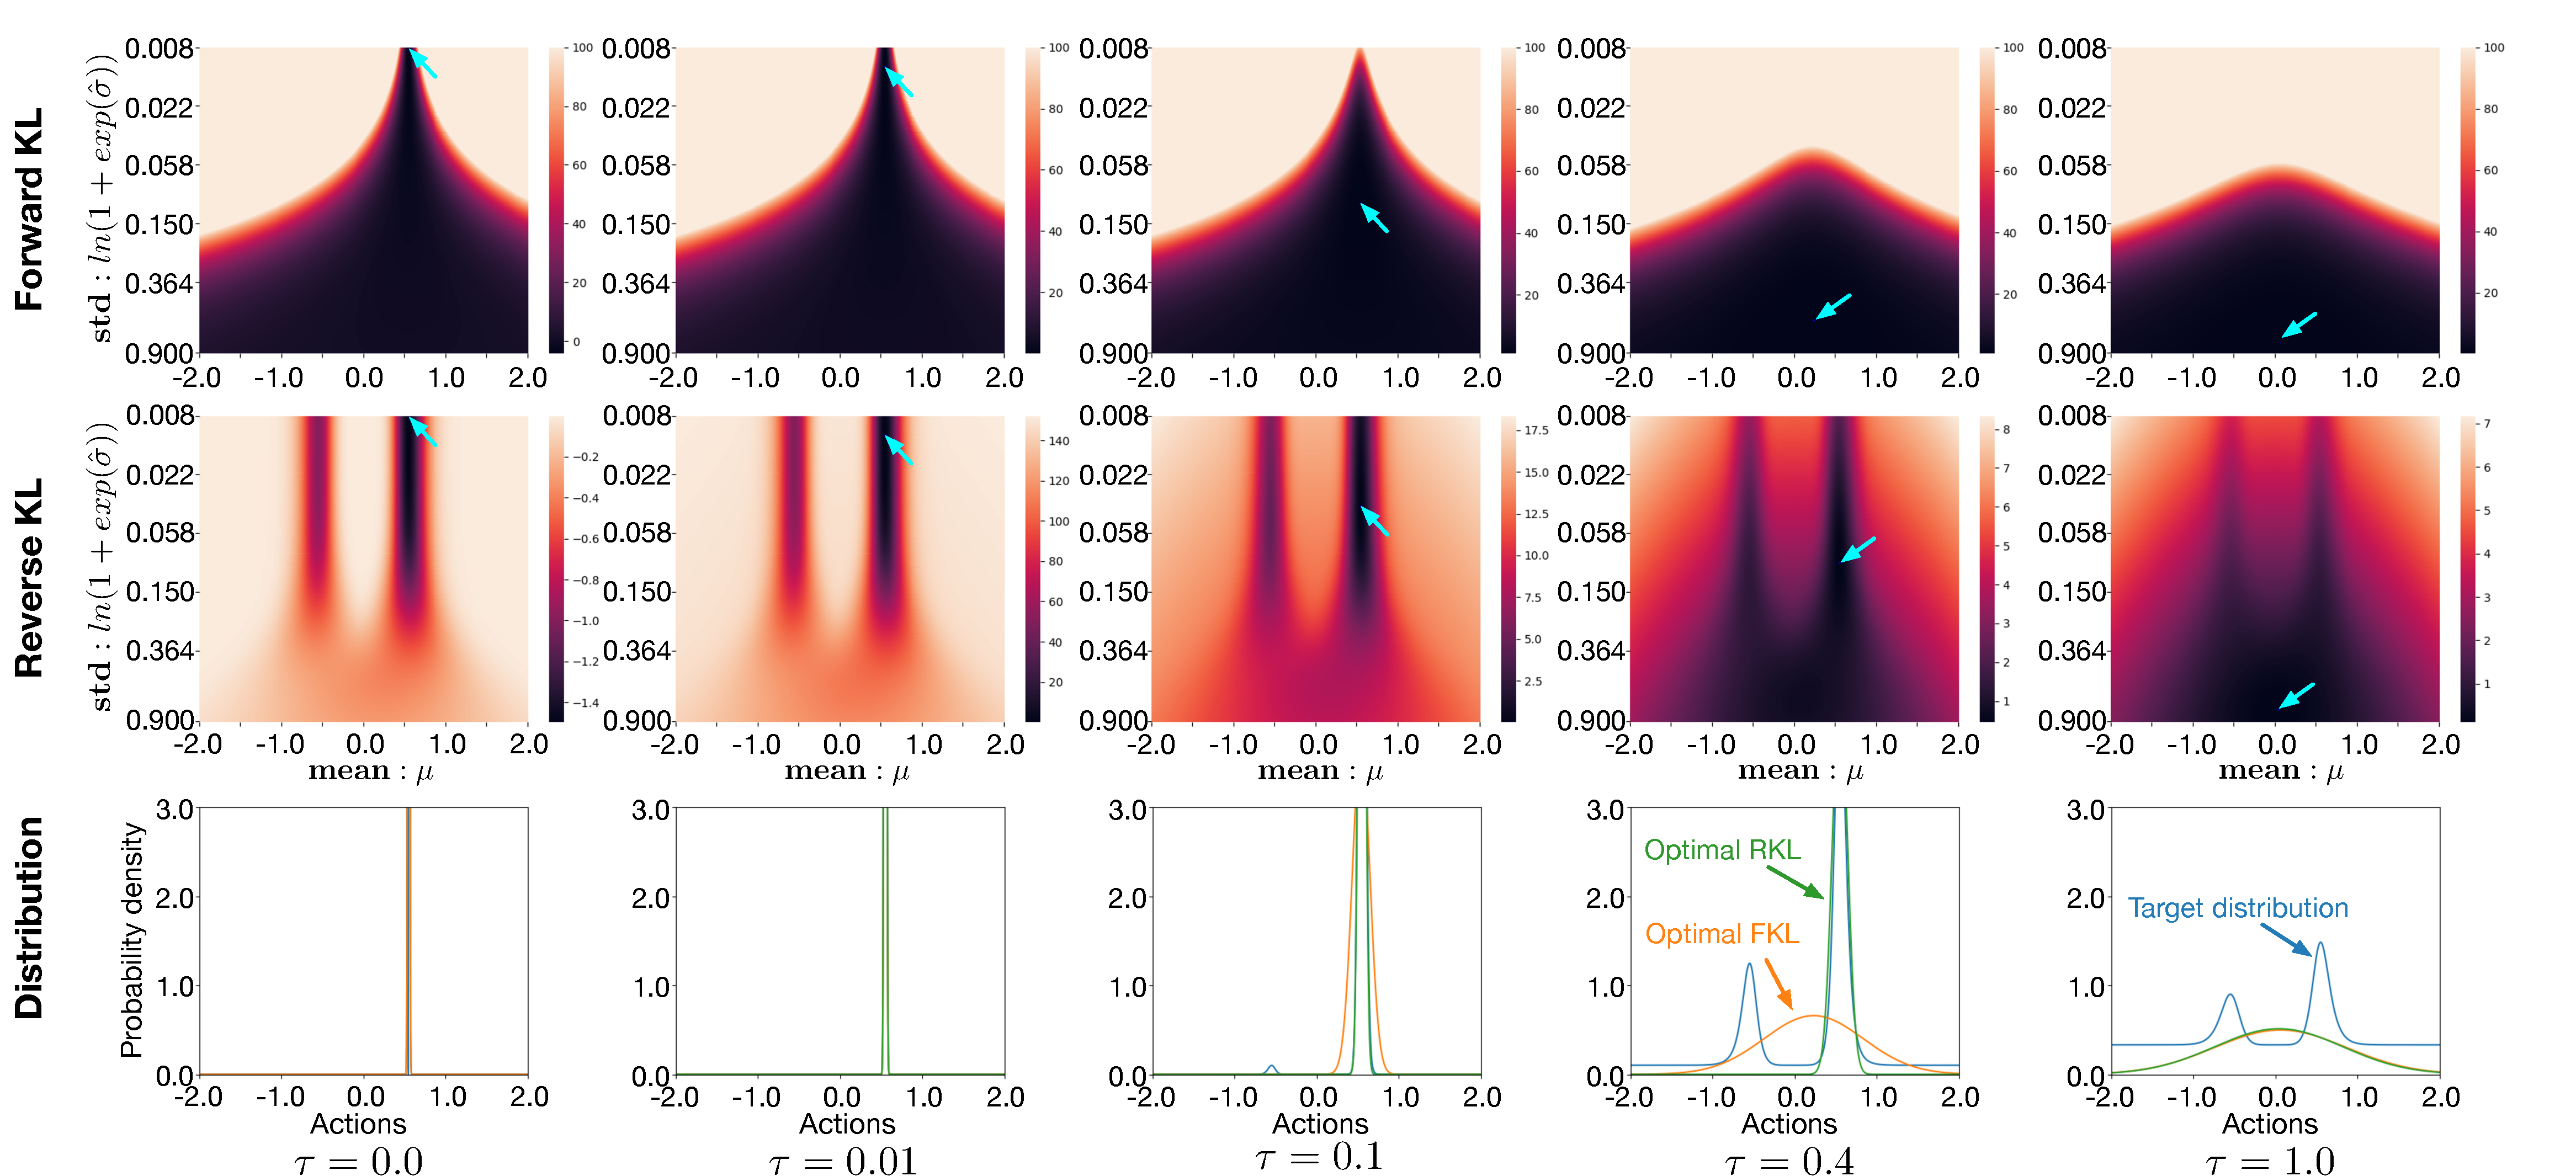
\includegraphics[width=0.99\columnwidth]{figs/bandit/trueQ/heatmaps/heatmap_combined.pdf}
    \caption{KL loss over mean and standard deviation across temperature. Note that the actual action taken applies $\tanh$ to the samples of the resulting distribution (i.e., the optimal mean is at $\tanh^{-1}(0.5) \approx 0.55$). FKL loss has been upper-bounded for better visualization of minima. Arrows indicate the global minimum.}
    \label{fig:bandit-heatmap}
\end{figure}

% \begin{figure}[!htb]
%   \centering
%   \begin{subfigure}[b]{1\linewidth}
%     \centering
%     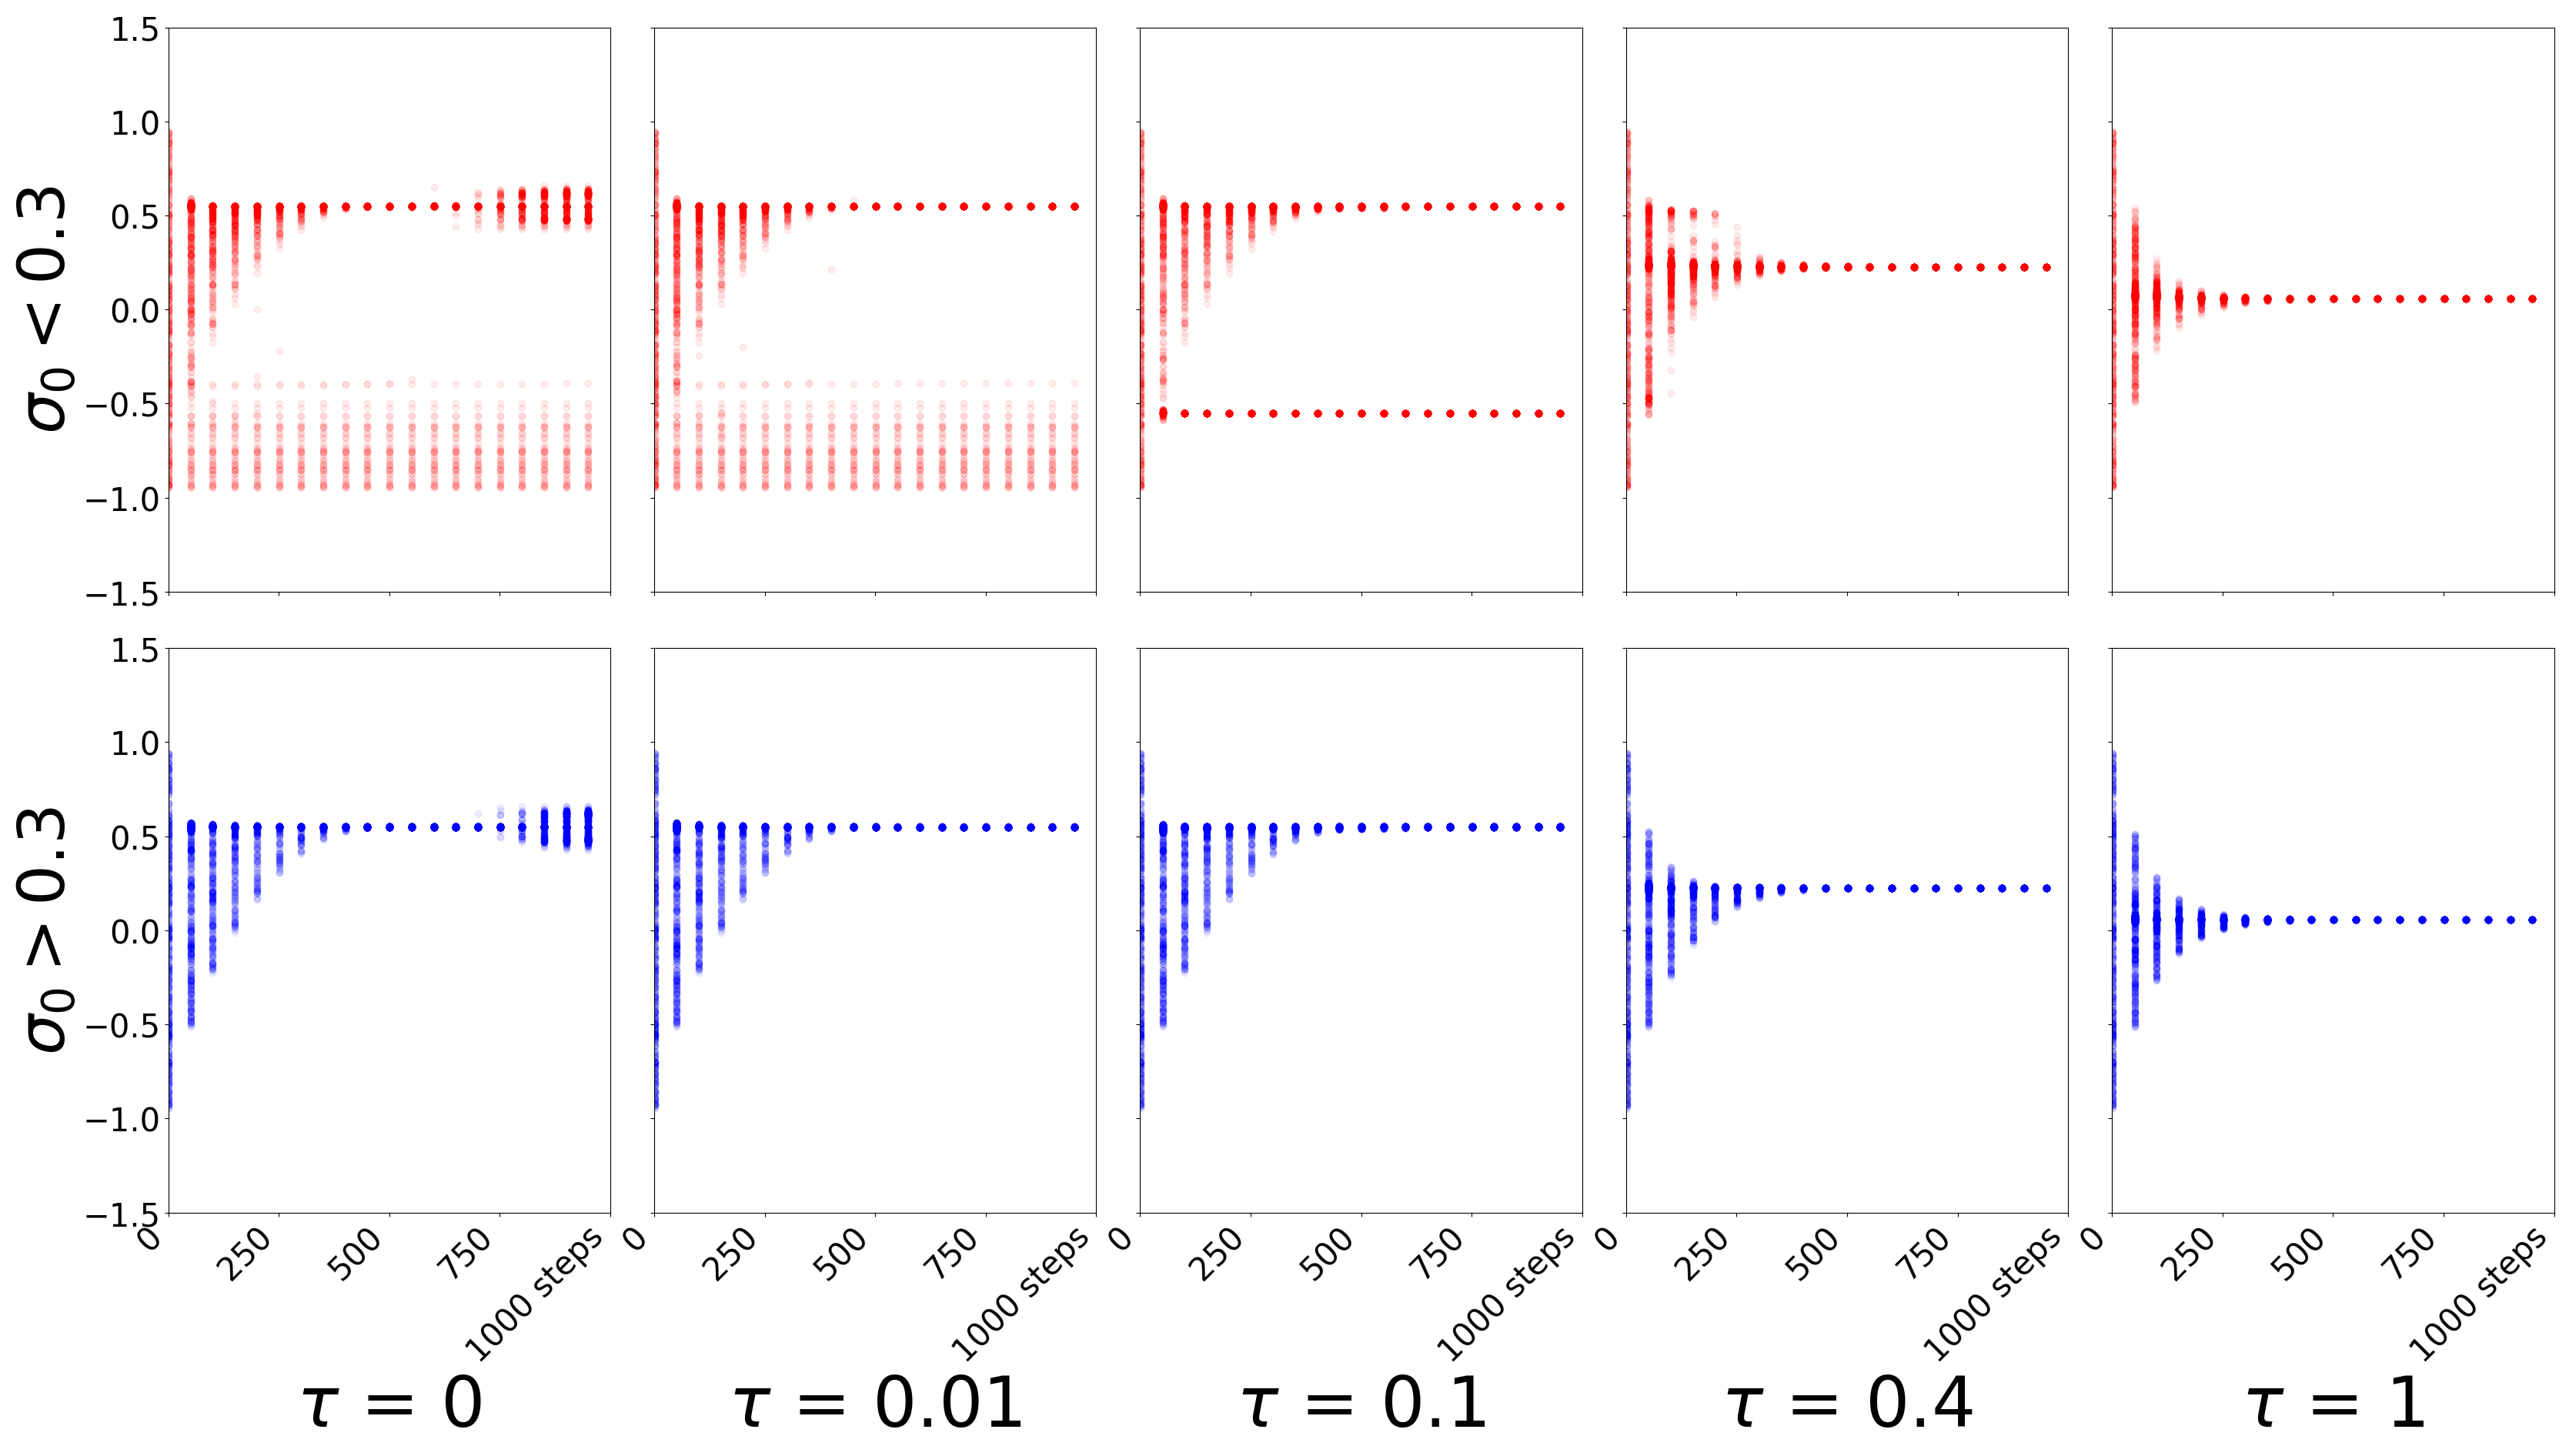
\includegraphics[width=\columnwidth]{figs/bandit/notlearnQ/modes=1/adam/mean_forward_optim=adam_modes=1_lr=0.01.png}
%     \caption{Forward KL.}
%     \label{fig:bandit-mean-forward-adam}
%   \end{subfigure}
  
%   \begin{subfigure}[b]{1\linewidth}
%     \centering
%     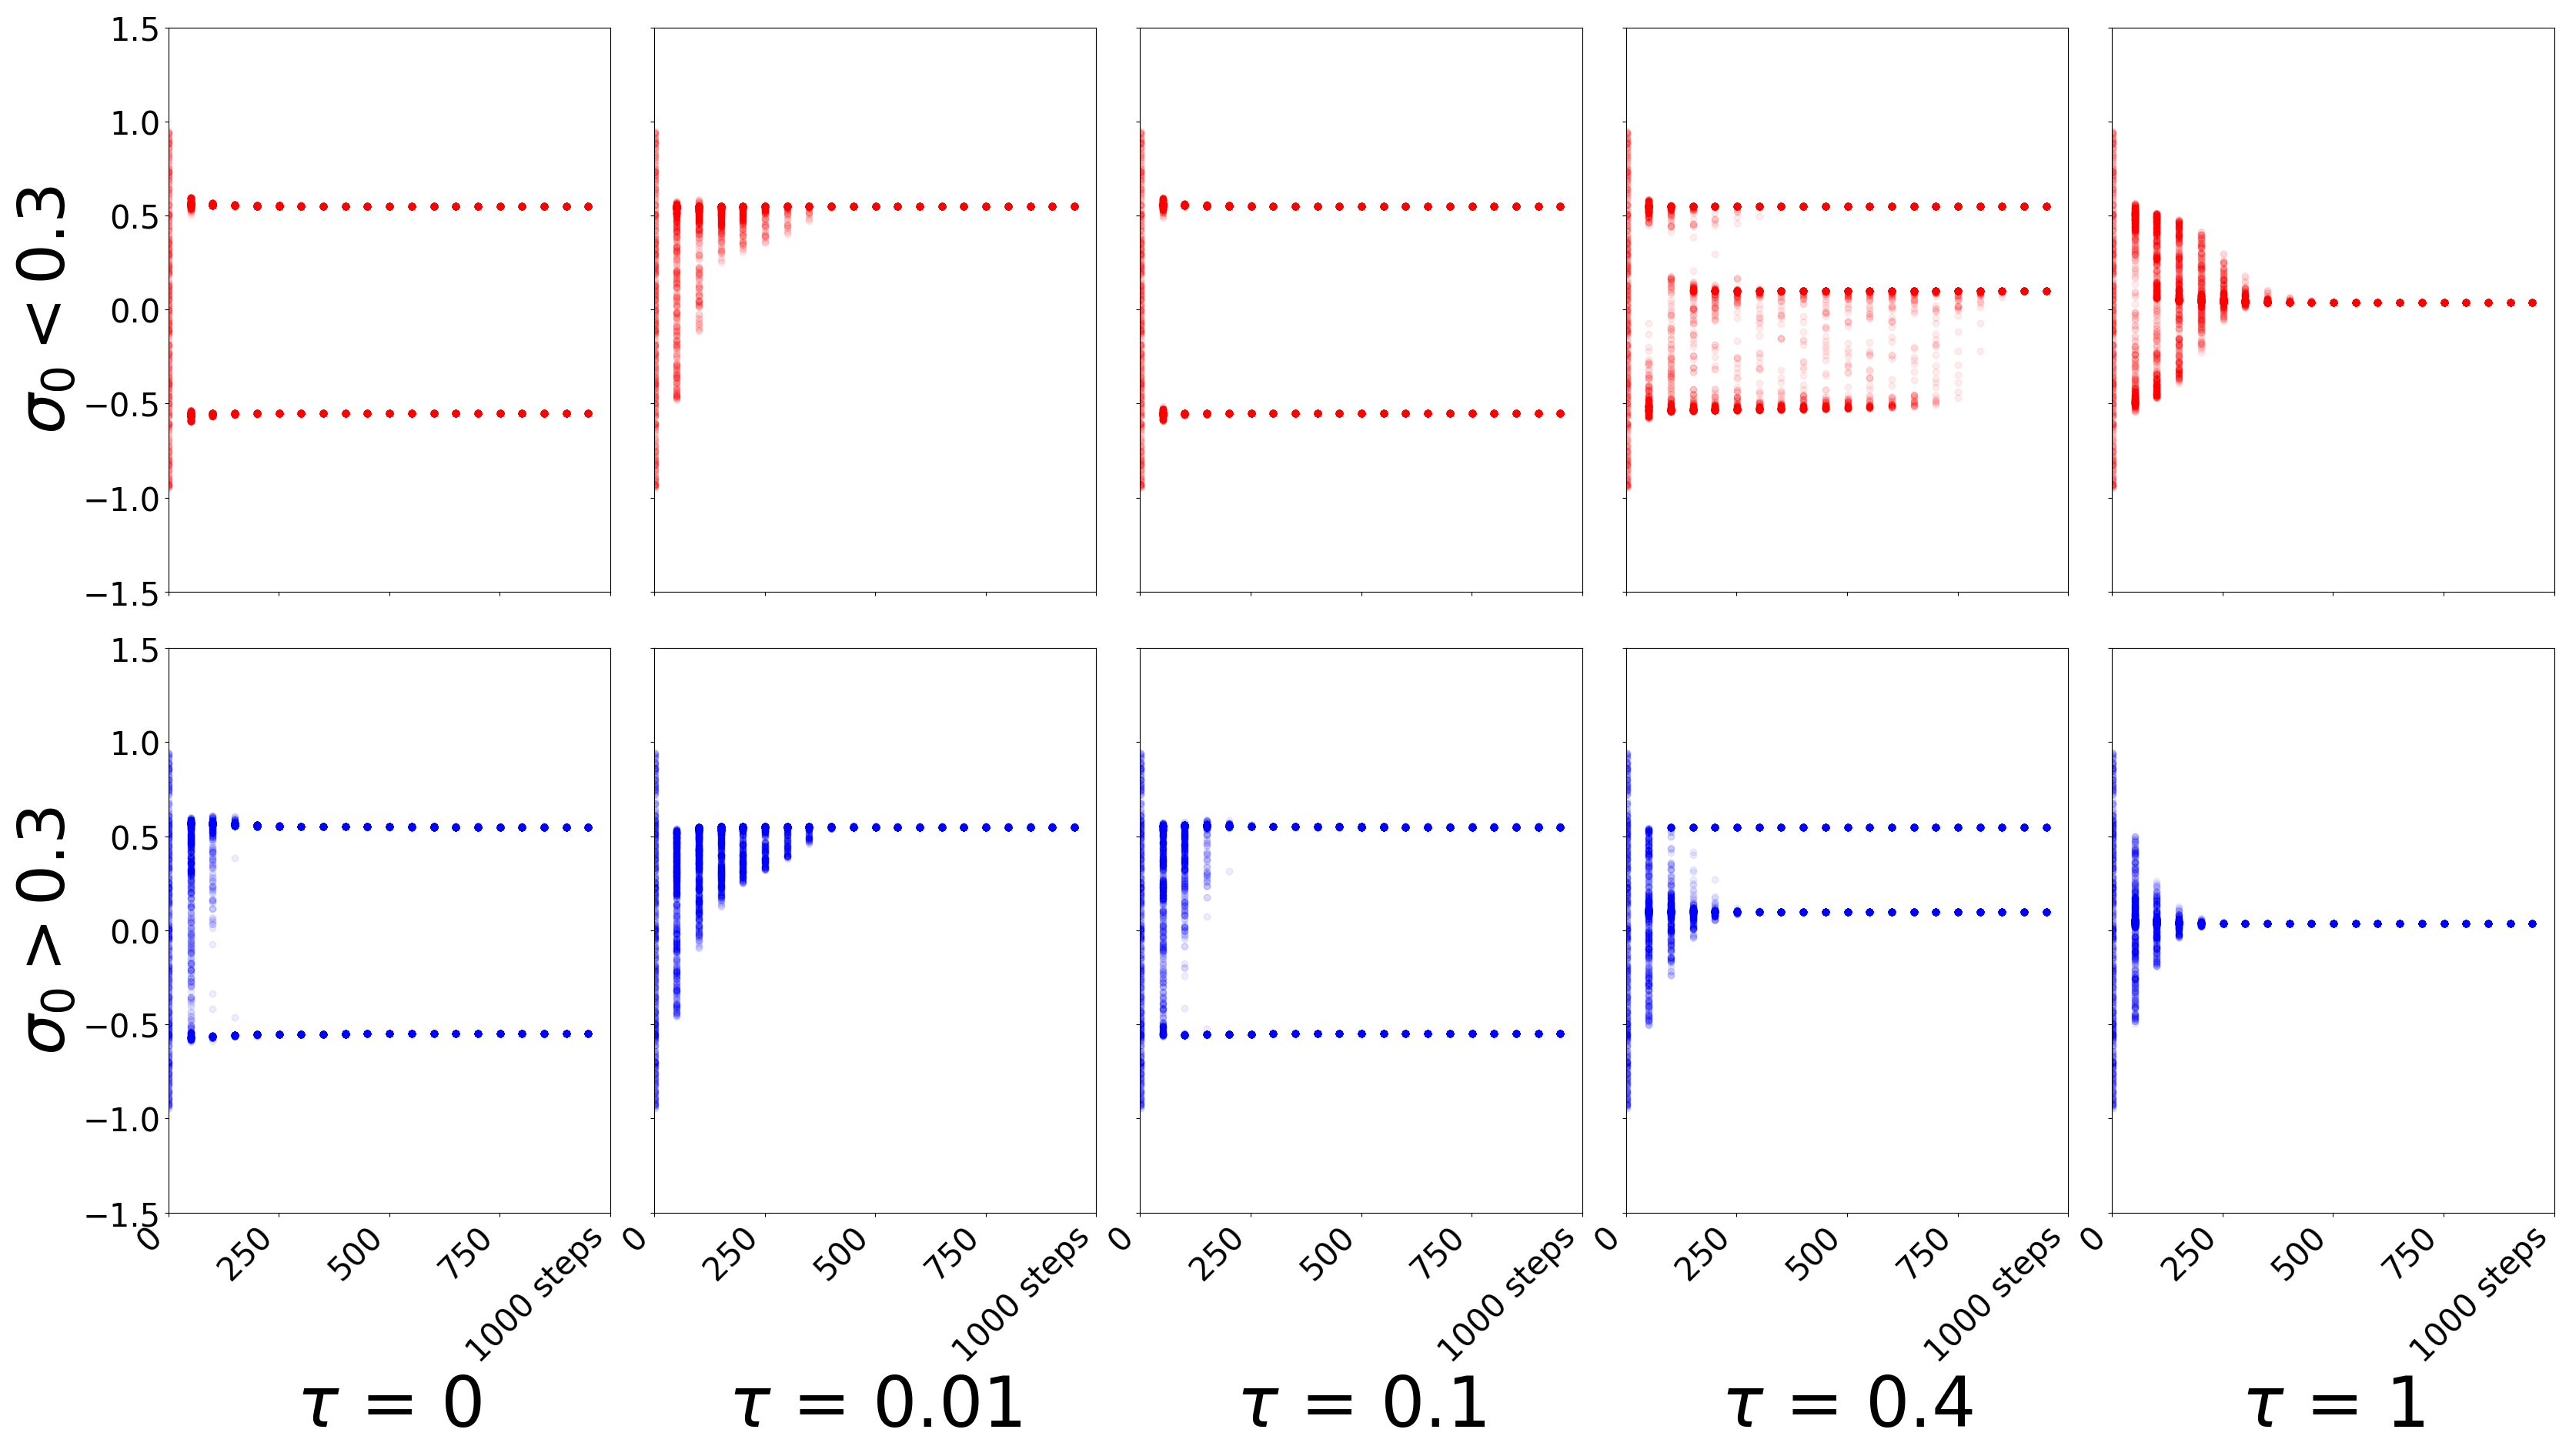
\includegraphics[width=\columnwidth]{figs/bandit/notlearnQ/modes=1/adam/mean_reverse_optim=adam_modes=1_lr=0.01.png}
%     \caption{Reverse KL.}
%     \label{fig:bandit-mean-reverse-adam}
%   \end{subfigure}
%   \caption{Each plot tracks the mean over 1000 gradient steps of each of 1000 iterates. Each iterate is represented as a translucent, coloured dot with alpha value $0.01$. Temperature is varied on the $x$-major-axis and initial standard deviation $\sigma_0$ is varied on the $y$-major axis. Colour-coded by $\sigma_0$.}
% \end{figure}

\subsubsection{Behaviour}
To confirm whether our intuitions about the smooth loss surface result in iterates that reach the global optimum, we visualize 1000 random (mean, standard deviation) iterates over 1000 gradient steps to minimize either the FKL or RKL. The mean is initialized uniformly in $(-0.95, 0.95)$ and $\hat{\sigma}$ is initialized uniformly in $(\log(\exp(0.1) - 1), \log(\exp(1) - 1))$, so that the initial standard deviation $\sigma_0$ is in $(0.1, 1)$. We only show one learning rate, but results are similar for different learning rates. From looking at \Cref{fig:bandit-mean-forward-rmsprop,fig:bandit-mean-reverse-rmsprop}, we observe the following.

\begin{figure}[!htb]
  \centering
  \begin{subfigure}[b]{1\linewidth}
    \centering
    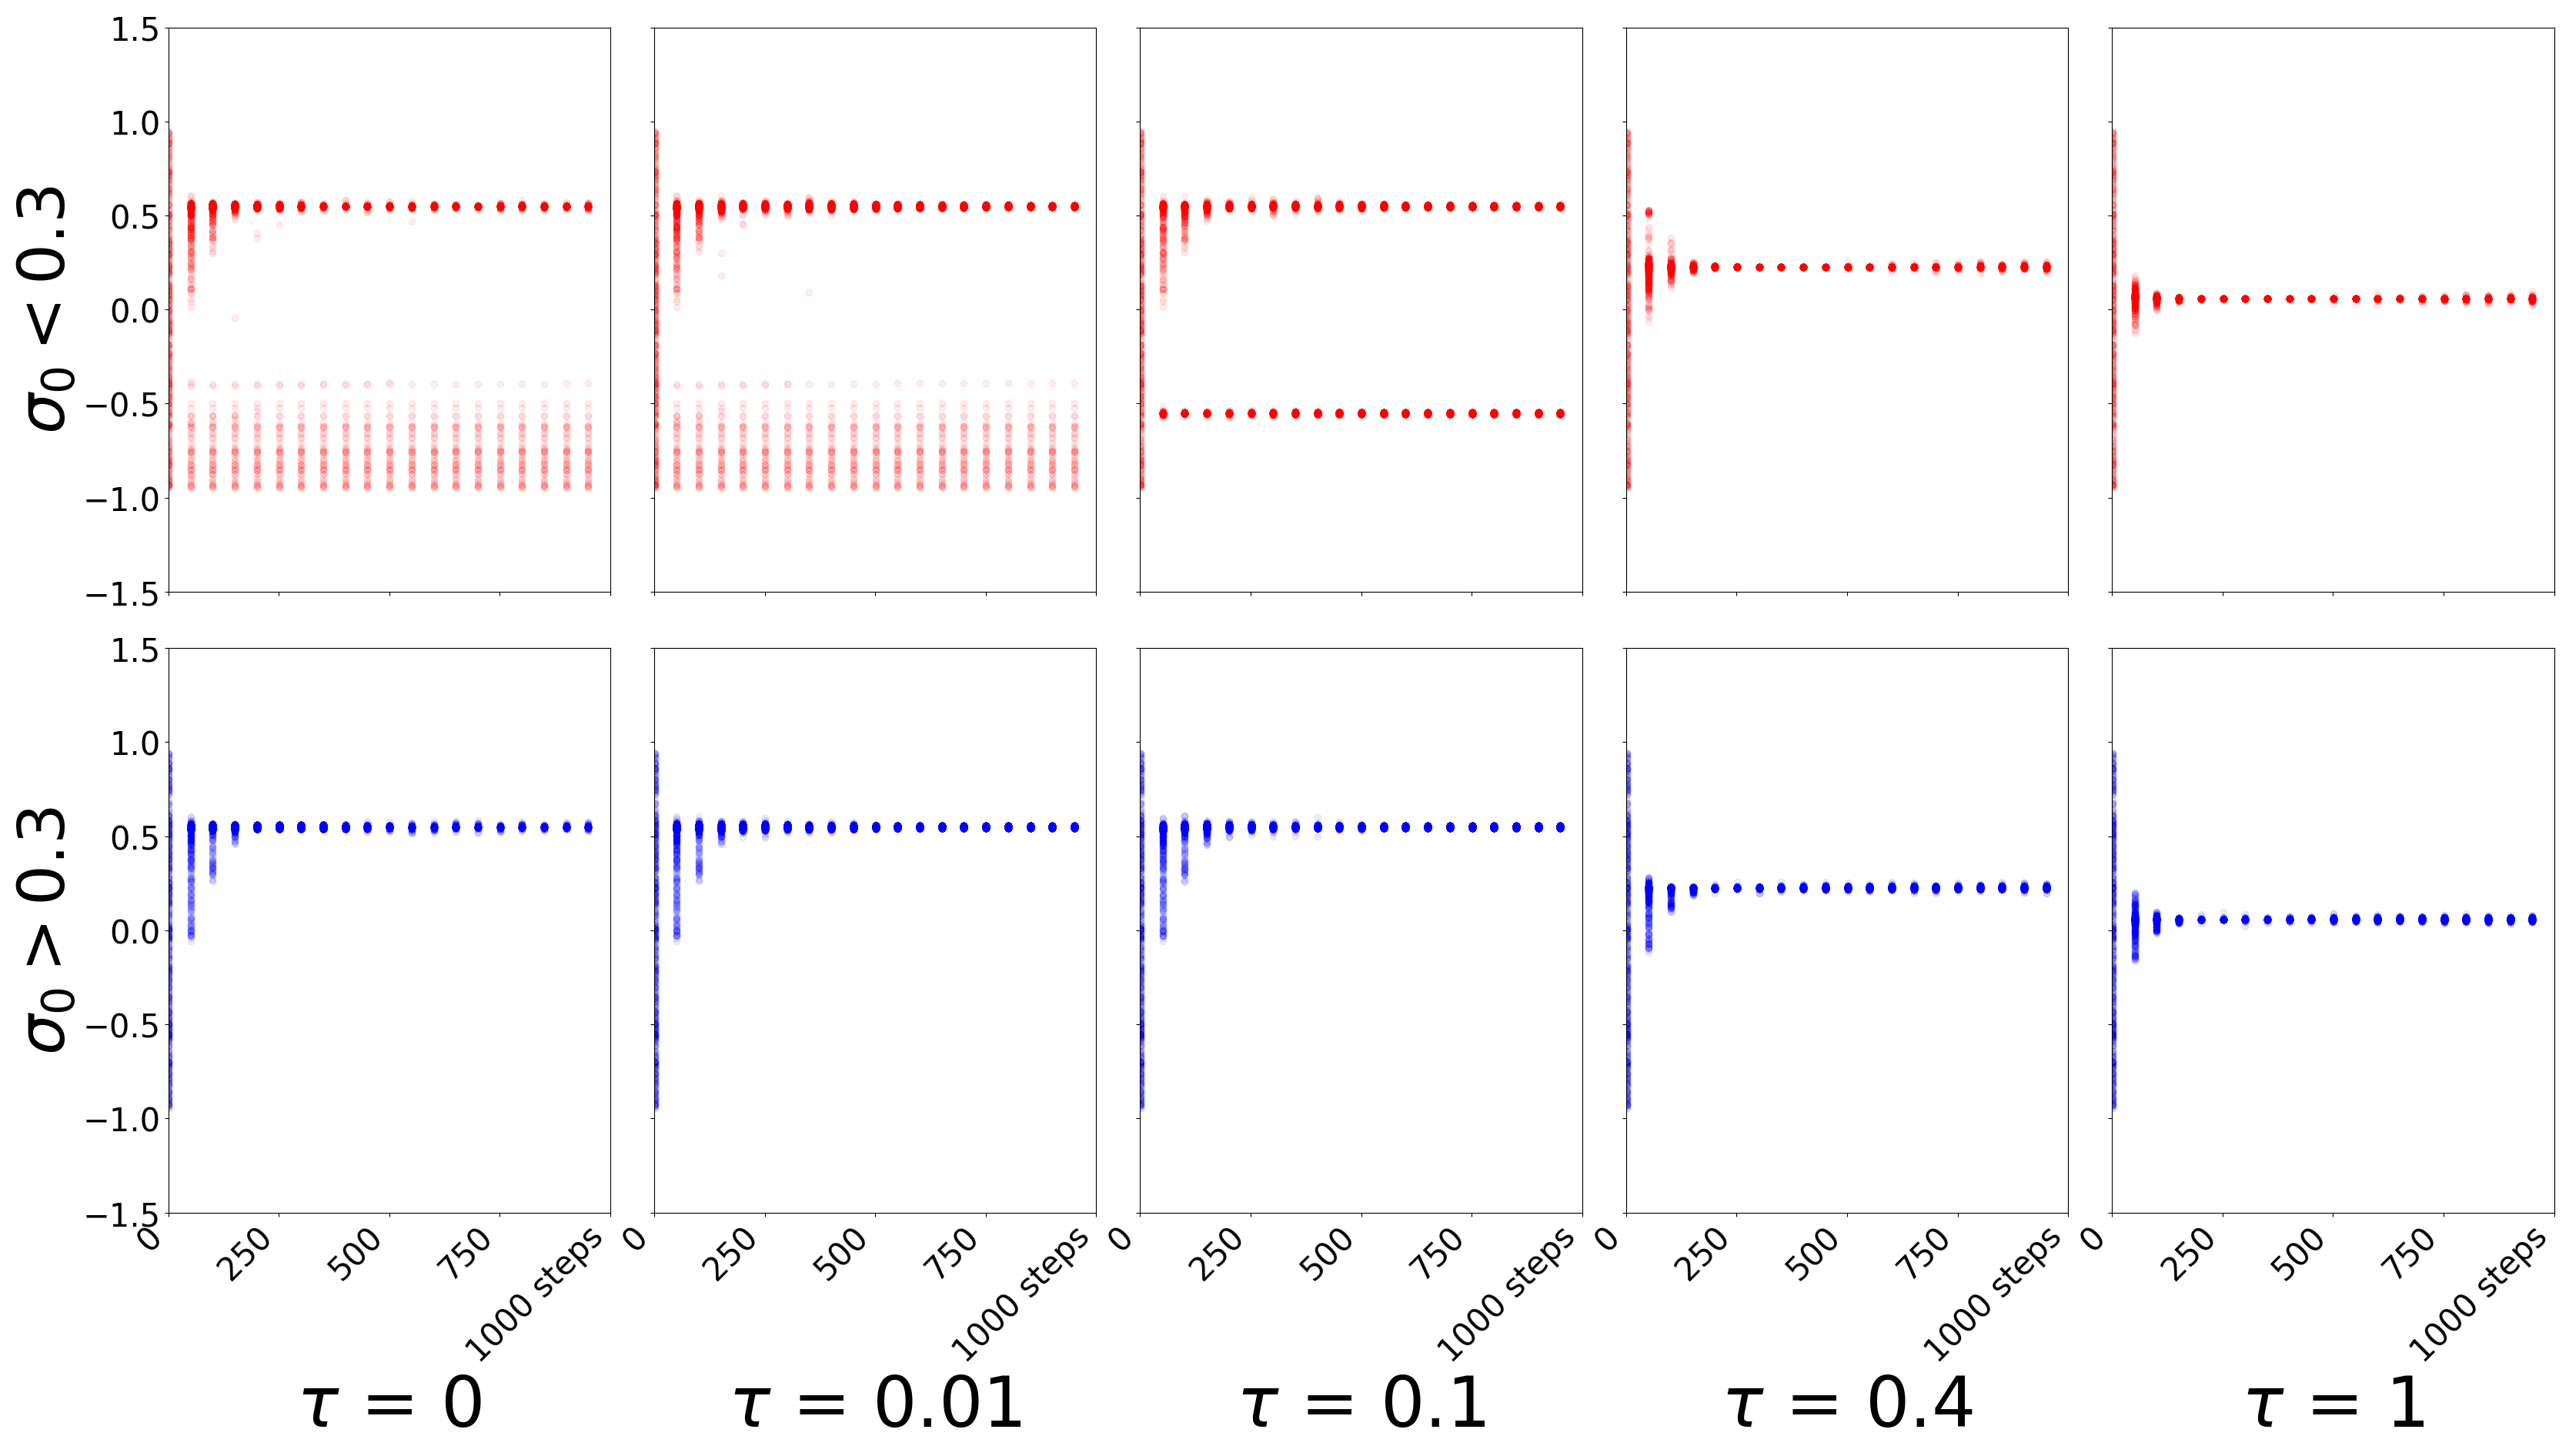
\includegraphics[width=\columnwidth]{figs/bandit/notlearnQ/modes=1/rmsprop/mean_forward_optim=rmsprop_modes=1_lr=0.01.png}
    \caption{Forward KL.}
    \label{fig:bandit-mean-forward-rmsprop}
  \end{subfigure}
  
  \begin{subfigure}[b]{1\linewidth}
    \centering
    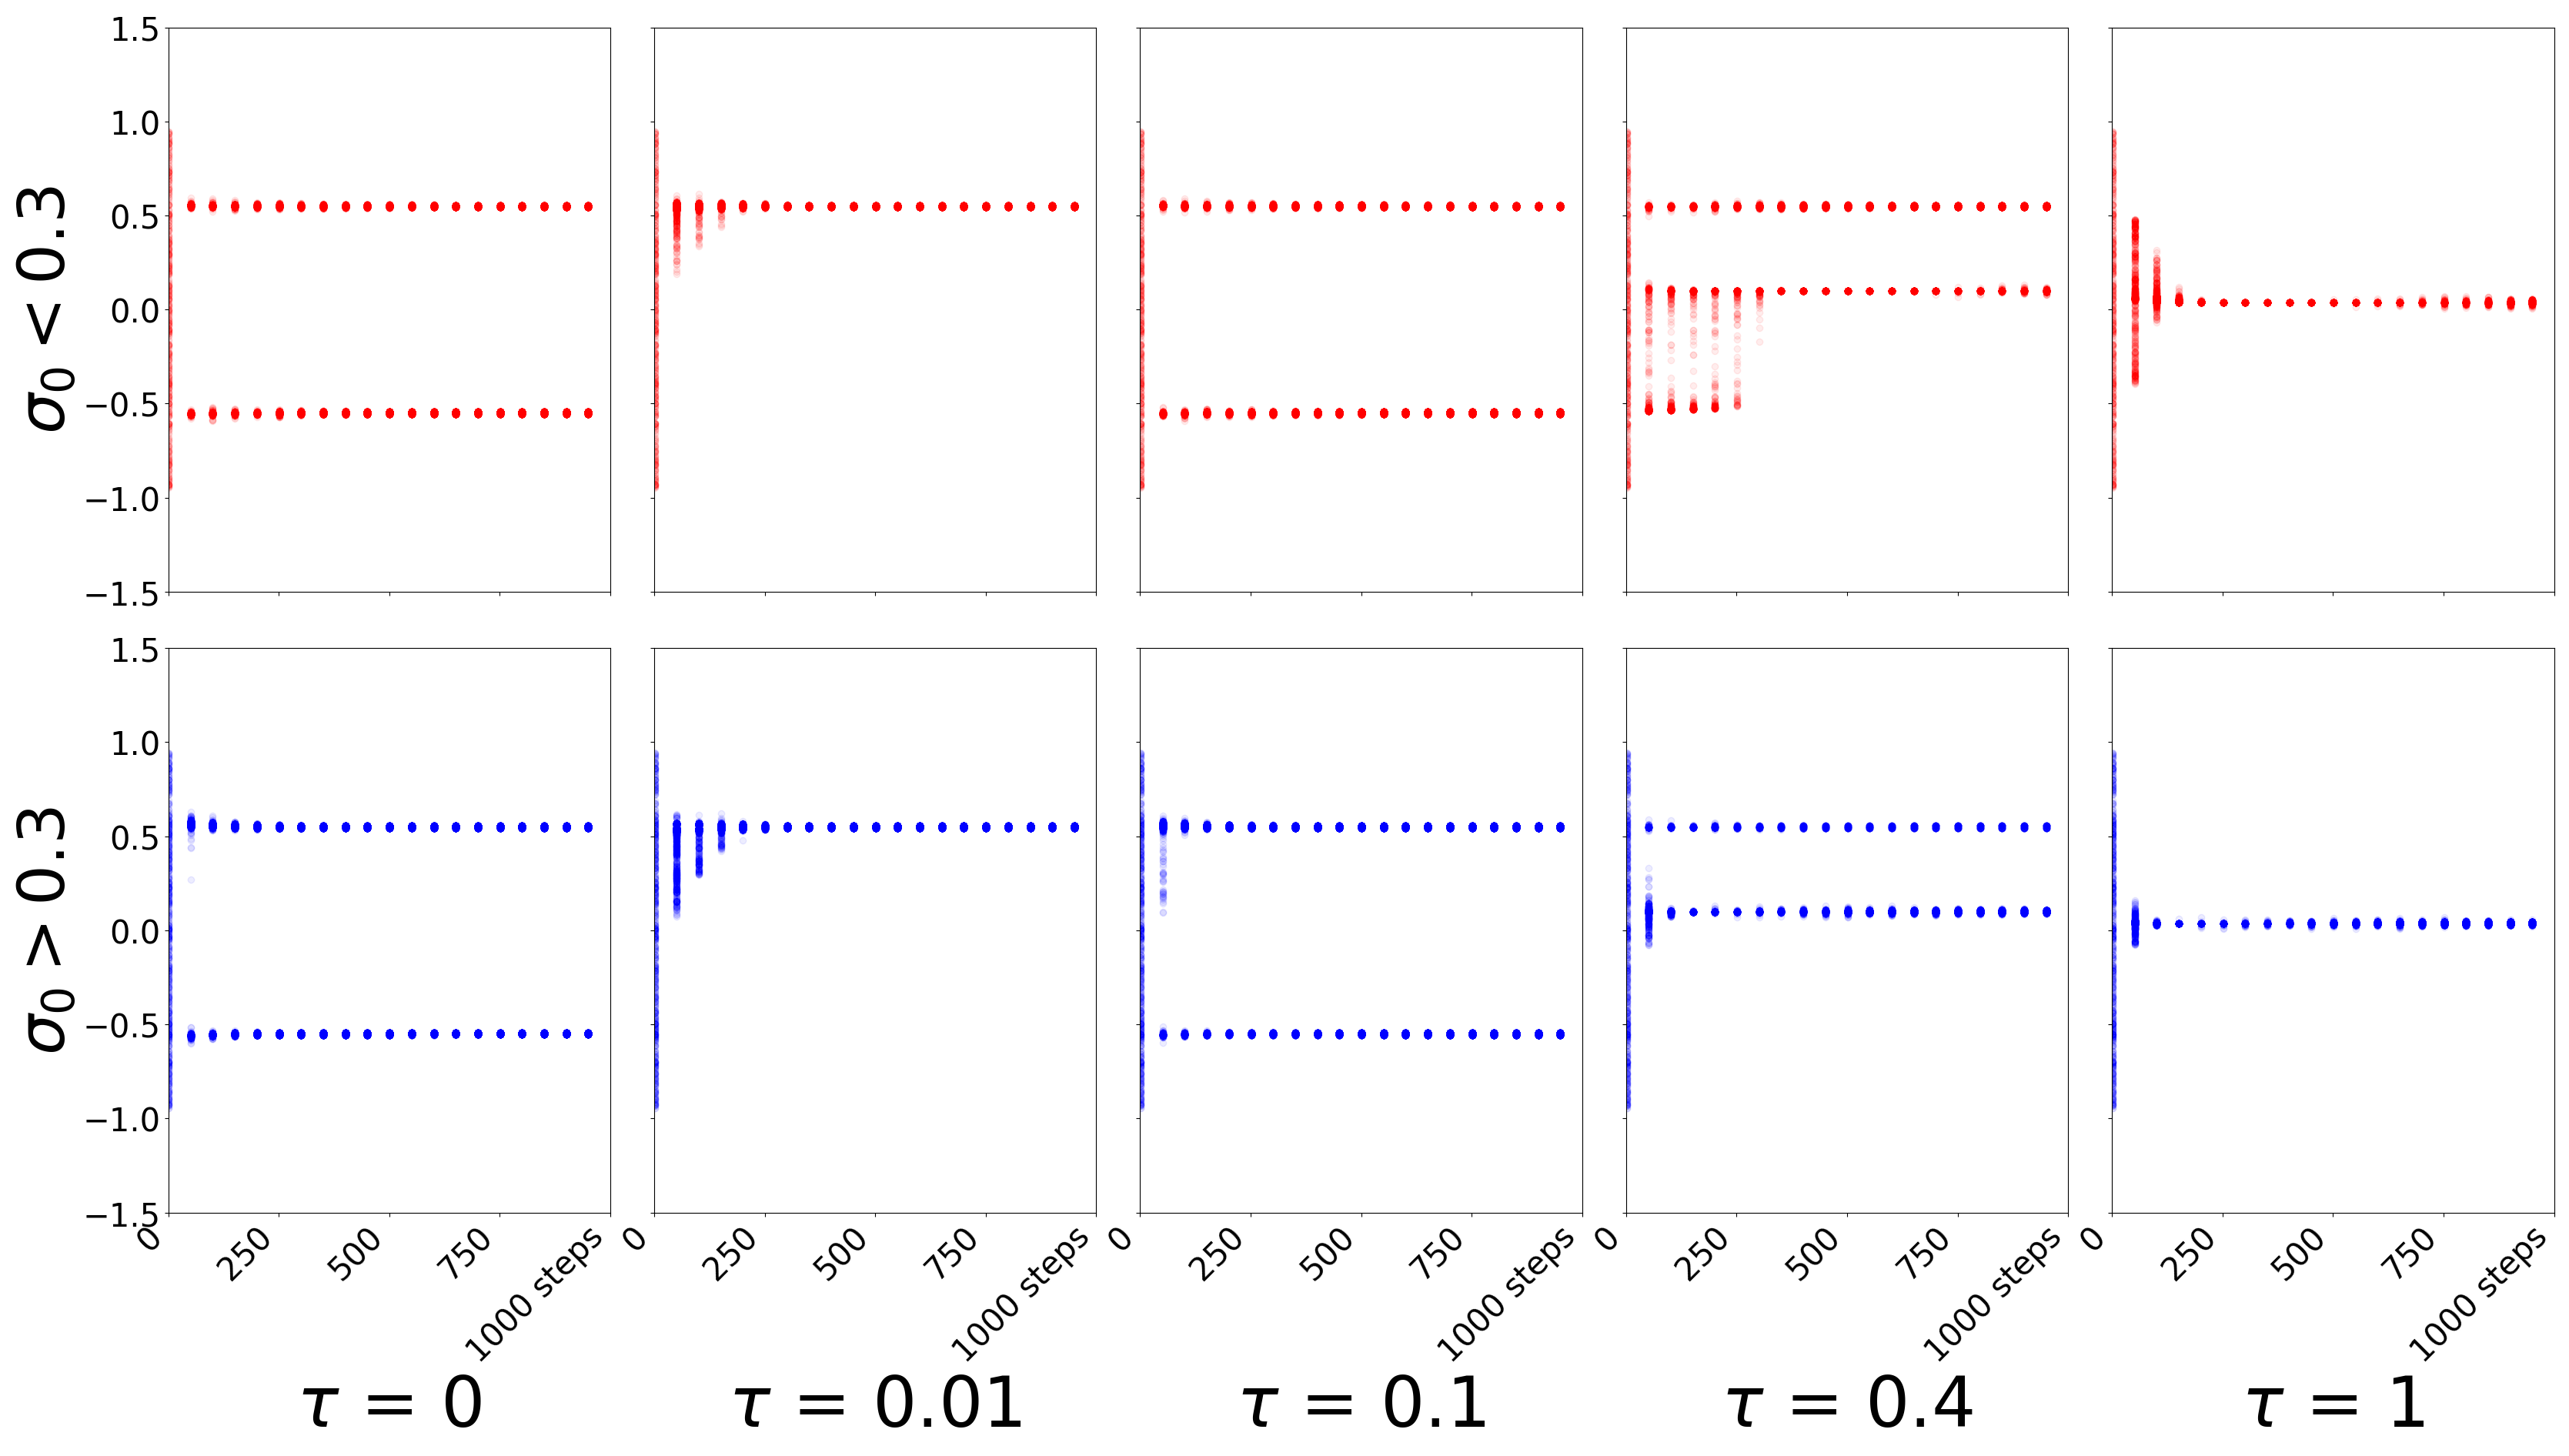
\includegraphics[width=\columnwidth]{figs/bandit/notlearnQ/modes=1/rmsprop/mean_reverse_optim=rmsprop_modes=1_lr=0.01.png}
    \caption{Reverse KL.}
    \label{fig:bandit-mean-reverse-rmsprop}
  \end{subfigure}
  \caption{Each plot tracks the mean over 1000 gradient steps of each of 1000 iterates. Each iterate is represented as a translucent, coloured dot with alpha value $0.01$. Temperature is varied on the $x$-major-axis and initial standard deviation $\sigma_0$ is varied on the $y$-major axis. Colour-coded by $\sigma_0$. Learning rate is 0.01.}
\end{figure}

\textbf{1)} FKL seems to facilitate more stable convergence of the iterates to the global optimum when $\sigma_0 > 0.3$. Indeed, within that setting, all iterates converge to a single optimum across all temperatures. 

\textbf{2)} Behaviour can vary across different standard deviation initializations. For $\tau < 0.4$, FKL iterates learn the optimal mode for all settings except when the $\sigma_0 < 0.3$. The achieved limit points of RKL iterates can differ depending on $\sigma_0$, such as with $\tau = 0.4$. 

\textbf{3)} RKL iterates converge to different local optima. The only case in which RKL iterates only converged to the optimal mode was for $\tau = 0.01$. 

\textbf{4)} At $\tau = 0.4$, FKL iterates converged to a point closer to zero than the RKL points, some of which remained at 0.5. This observation is consistent with our visualization of the loss surface, where the global optimum of the FKL loss moved to 0 more quickly than did the global optimum of the RKL loss. 
% 

These results are generally consistent with the FKL and RKL heatmaps, suggesting that for large enough $\sigma_0$, the FKL has a much smoother optimization landscape that directs iterates to the global minimum, but the global minimum might be suboptimal with respect to the original target distribution. One discrepancy with the visualization of the loss surfaces, however, is that both RKL and FKL exhibited limit points that do not appear to correspond to any optima on the heatmaps. In particular, FKL with $\sigma_0 < 0.3$ and $\tau \leq 0.1$ have iterates that stay in a neighbourhood away from 0, while the RKL at $\tau = 0.4$ and $\sigma_0 < 0.3$ has iterates that converge to 0. The same phenomenon was also present with both smaller and larger learning rates, and with RMSprop and SGD. While our initial surprise at the RKL limit point may be due to a limitation of our heatmaps---indeed, 0 might be a local minimum that is hard to distinguish amidst the dark area of \Cref{fig:bandit-heatmap}---the FKL limit point is more puzzling. The area around the line $\sigma = 0.3$ in \Cref{fig:bandit-heatmap} for $\tau = 0.01$ seems not to contain a local optimum. 

An earlier version of this experiment used integration points within the range $[-0.98, 0.98]$, rather than using all points but \{-1, 1\}. In this earlier setting, RKL iterates often diverged for $\sigma_0 > 0.3$ while FKL iterates maintained the same behaviour, suggesting that FKL is more robust to this type of bias than RKL. We comment more on the effect of numerical integration error in \Cref{sec:stochastic-microworld}. %Divergence of iterates in RKL occurs for larger $\sigma_0$, at $\tau = 0.01, 0.1$ where the iterates seem to fall into the suboptima at bottom corners of the heatmap. (Visualization of the gradients can be found in Appendix G)


\subsection{Switch-Stay}
Given our previous results, we might expect the FKL to perform better. If FKL iterates can reach the global optimum more easily, surely those policies would be better than policies updated under the RKL? One important factor, which we explore further below, is that the global minimum of the FKL objective may not correspond well with the optimal solution of the original, unregularized objective. 

We investigate the behavior of iterates when there is more than one state: the Switch-Stay environment. As a simple instantiation of the full RL problem, we are interested in understanding any possible differences between FKL and RKL in the presence of short-term/long-term trade-offs. In particular, on Switch-Stay, from state 0 one should incur a short-term penalty by switching to state 1 to maximize return, given that $\gamma = 0.9$.

Another reason why we selected the Switch-Stay environment is for ease of visualization. Since the MDP has only two states, one can plot any value function as a point on a 2-dimensional plane. In particular, one can view the entire space of value functions, shown recently to be a polytope in the discrete-action setting \citep{dadashi2019value}. Plotting the value function corresponding to a policy as it changes over time allows us to view the progress of an algorithm and avoids the stochasticity inherent in performing rollouts and plotting learning curves.

To plot the boundary of the value function polytope in Switch-Stay, we plot the value functions corresponding to semi-deterministic policies (i.e., policies that are deterministic in at least one state) \citep{dadashi2019value}. Given a policy $\pi$, the value function $\vpi$ is calculated exactly as $(I - \gamma P_\pi)^{-1}r_\pi$, where $P_\pi$ and $r_\pi$ are respectively the transition matrix and the reward function induced by $\pi$. 

In the continuous version of switch-stay, we treat any action $ \leq 0$ as stay, and any action $ > 0$ as switch. To calculate the value function corresponding to a continuous policy $\pi$, we convert $\pi$ to an equivalent discrete policy $\pi_{\mathrm{discrete}}$ of the underlying discrete MDP. The conversion requires the calculation of the probability that $\pi$ outputs an action $\leq 0$ in each state, which we do with numerical integration of the policy PDF. We then calculate the value function of $\pi$ as $(I - \gamma P_{\pi_{\mathrm{discrete}}})^{-1}r_{\pi_{\mathrm{discrete}}}$.

For the hard FKL, we require access to the greedy action of the action-value function. In the continuous-action setting, this greedy action is usually infeasible to obtain. For the purposes of this experiment, if the greedy action is stay, we represent it in $[-1, 1]$ by drawing a uniform random number from $[-1, 0]$. If the greedy action is switch, we represent it as a uniform random number in $[0, 1]$. This design choice is meant to simulate noisy access to the greedy action in practice. 

As the policy is tabular in the states, we simply use the mean KL across states as the loss. 

\subsubsection{Behaviour}
% \paragraph{Optimization Path on Continuous Switch-Stay}
 %Based on our results for the bandit setting, we run three sets of experiments with three different standard deviation initializations, such that $\sigma_0$ is in $(0.1, 0.3), (0.3, 1)$. 
For all of these experiments, we initialized means in the range $(-0.95, 0.95)$. All experiments are run for 500 gradient steps and each experiment has 1000 iterates. We plot the value function of the final policy for each iterate and experiment in \Cref{fig:cont-ss-poly-0.005,fig:cont-ss-poly-0.01}, by visualizing the value function polytope \citep{dadashi2019value}. 

\begin{figure}[!htb]
  \centering
  \begin{subfigure}[b]{0.6\linewidth}
    \centering
    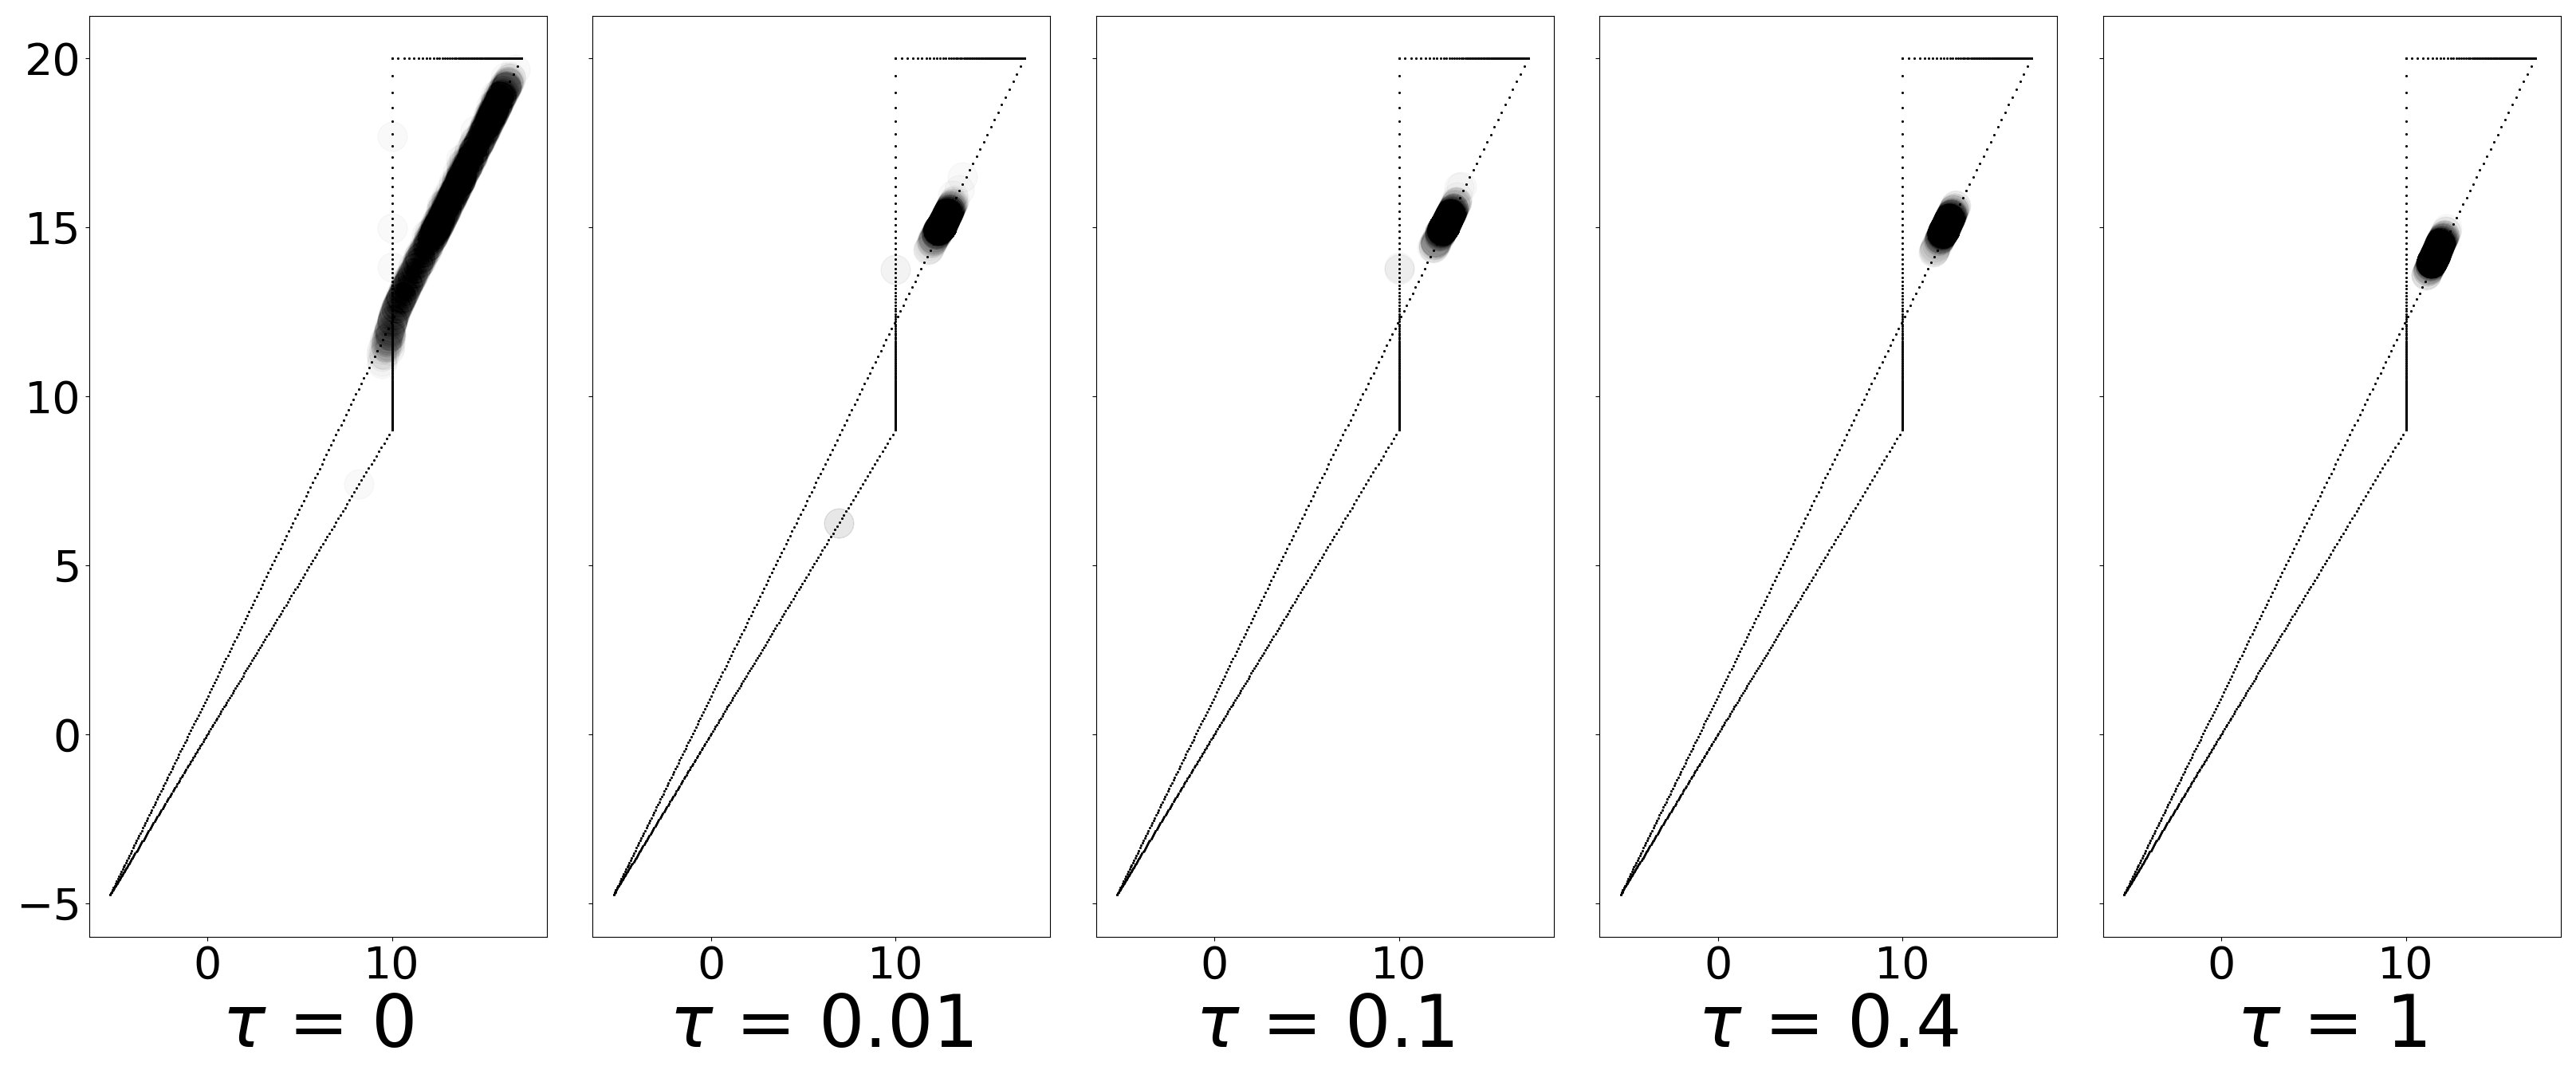
\includegraphics[width=\columnwidth]{figs/continuous-switch-stay/notlearnQ/polytope_forward_optim=rmsprop_lr=0.005.png}
    \caption{Forward KL, learning rate = $0.005$.}
    \label{fig:cont-switch-stay-forward}
  \end{subfigure}%\hspace{15pt}
  
  \begin{subfigure}[b]{0.6\linewidth}
        \centering
        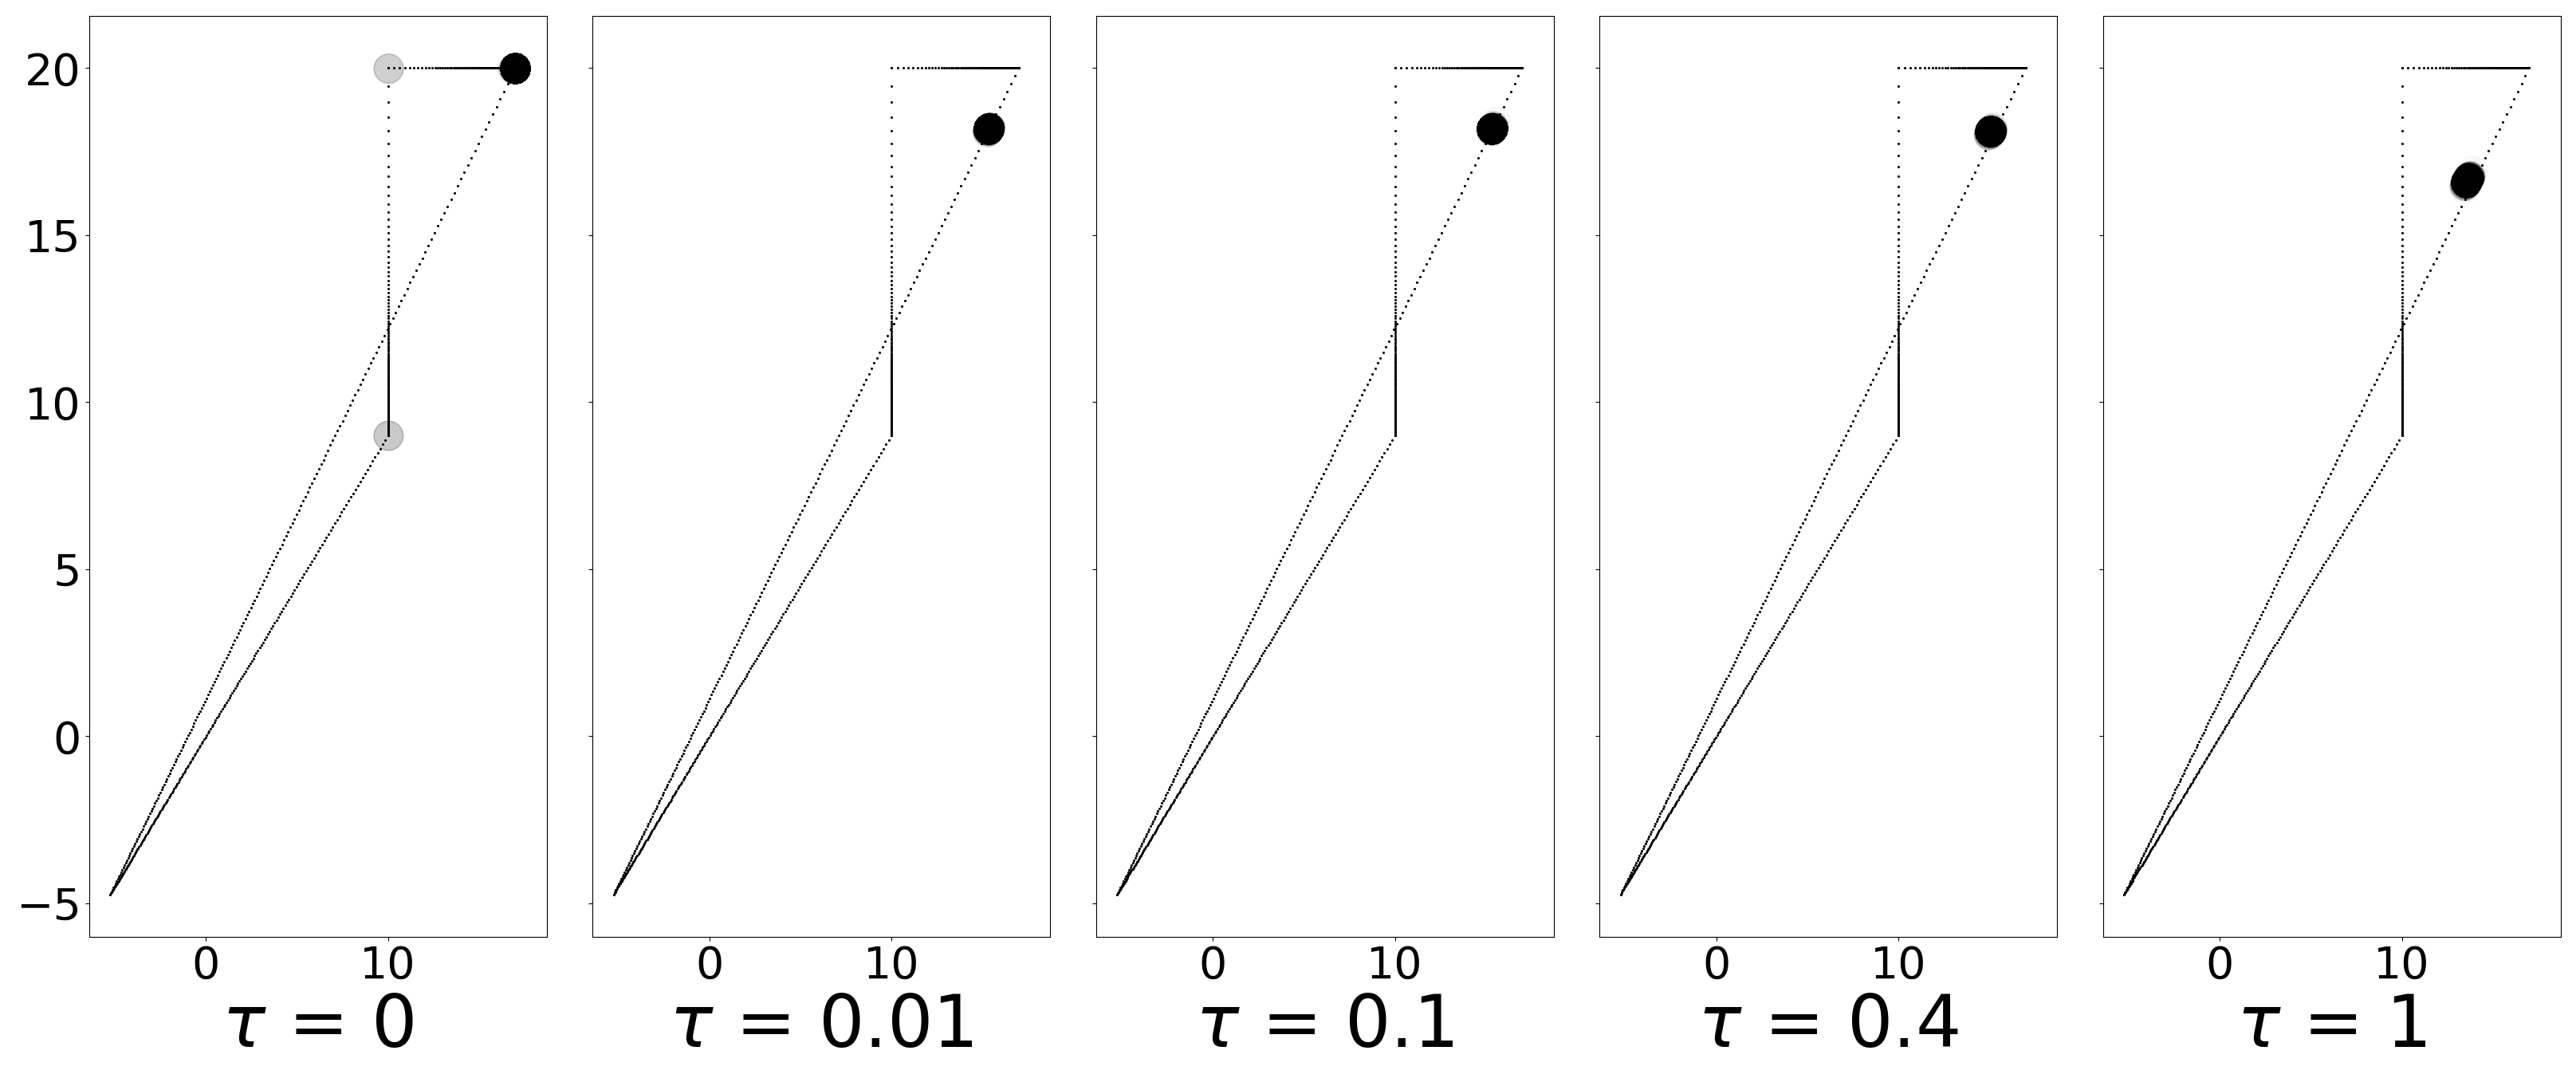
\includegraphics[width=\columnwidth]{figs/continuous-switch-stay/notlearnQ/polytope_reverse_optim=rmsprop_lr=0.005.png}
        \caption{Reverse KL, learning rate = $0.005$.}
        \label{fig:cont-switch-stay-reverse}
  \end{subfigure}
  \caption{Each subplot plots the final value functions on the continuous version of switch-stay after 500 gradient steps with $\gamma = 0.9$ for 1000 iterates. The top-right corner of the polytope in each subplot is the optimal value function and the bottom-left corner is the pessimal value function. Each iterate is represented by a translucent dot with alpha value $0.01$. Using RMSprop. Temperature is varied on the $x$-major-axis.}
  \label{fig:cont-ss-poly-0.005}
\end{figure}

\begin{figure}[!htb]
    \centering
    \begin{subfigure}{0.6\linewidth}
    \centering
    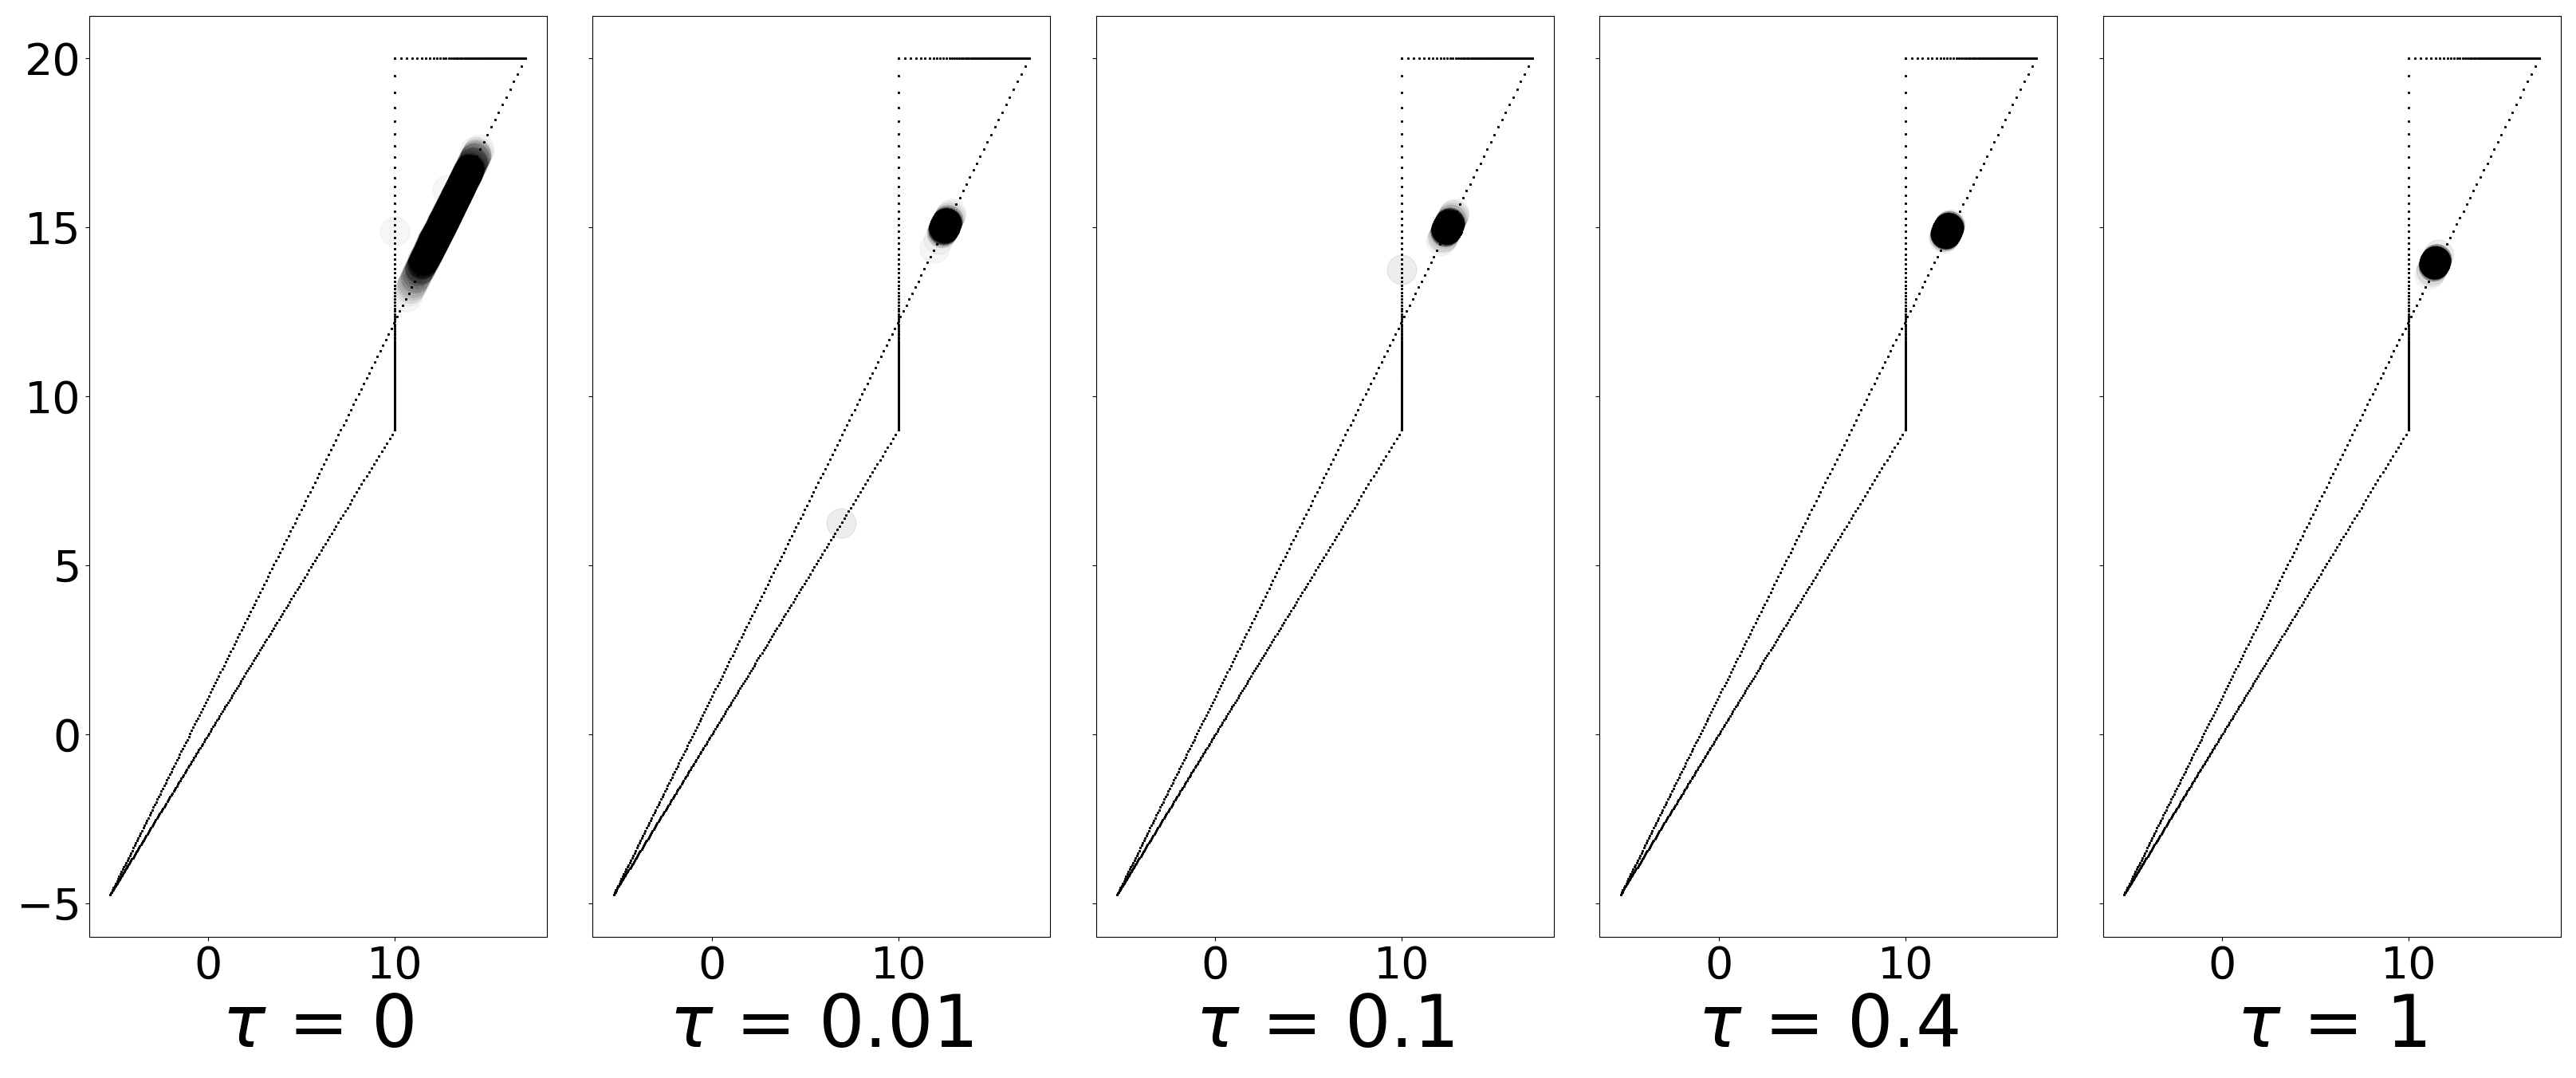
\includegraphics[width=\columnwidth]{figs/continuous-switch-stay/notlearnQ/polytope_forward_optim=rmsprop_lr=0.01.png}
    \caption{Forward KL, learning rate = $0.01$.}
    \label{fig:cont-switch-stay-forward-0.01}
  \end{subfigure}%\hspace{15pt}
  \begin{subfigure}[b]{0.6\linewidth}
        \centering
        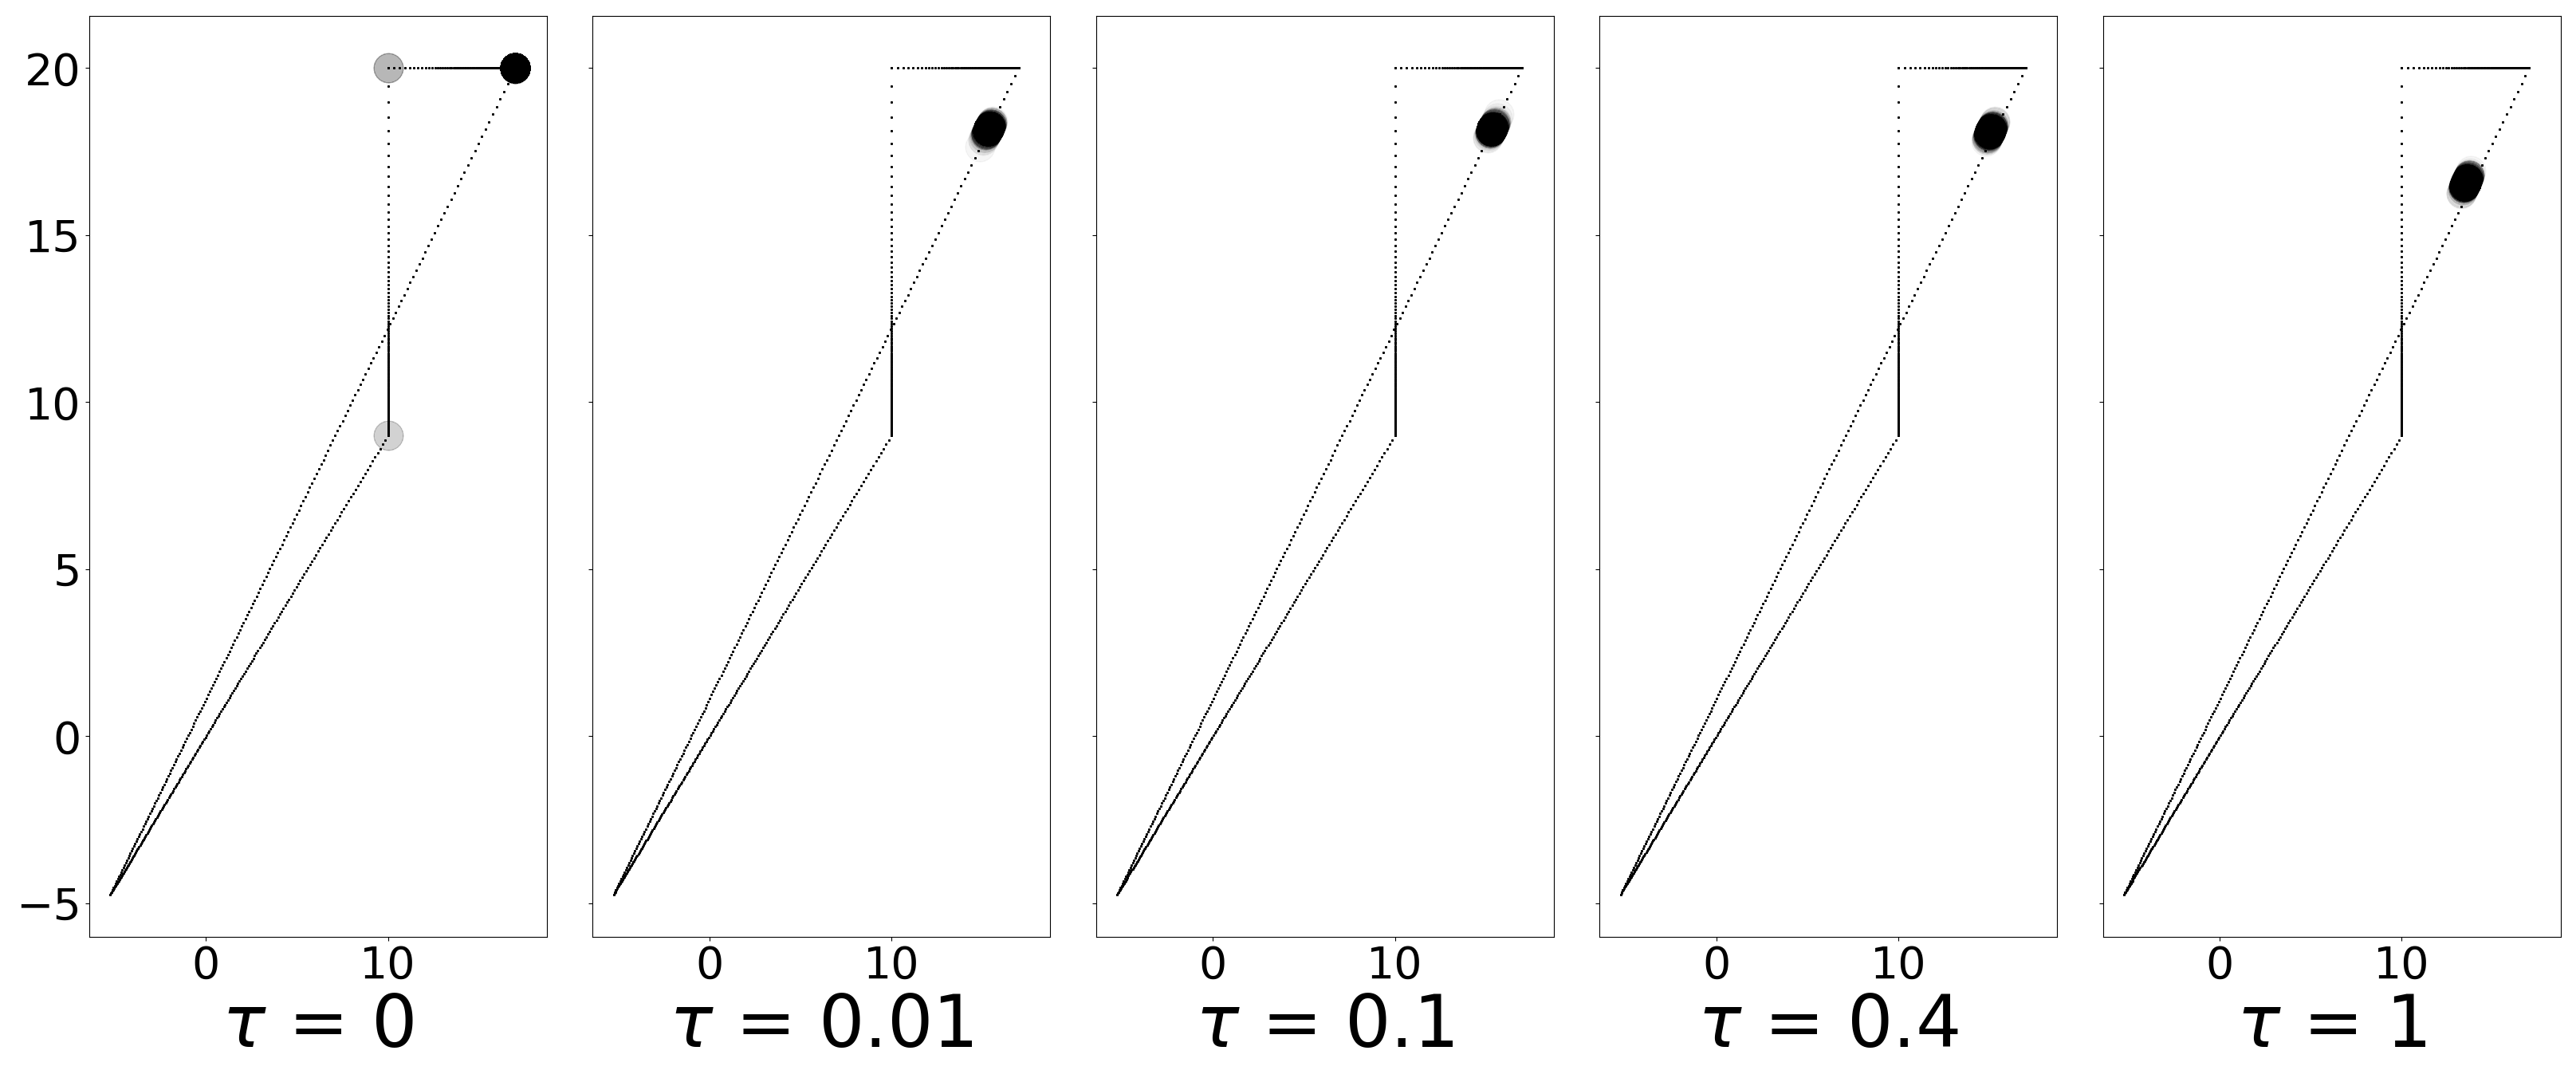
\includegraphics[width=\columnwidth]{figs/continuous-switch-stay/notlearnQ/polytope_reverse_optim=rmsprop_lr=0.01.png}
        \caption{Reverse KL, learning rate = $0.01$.}
        \label{fig:cont-switch-stay-reverse-0.01}
  \end{subfigure}
  \caption{See \Cref{fig:cont-ss-poly-0.005}.}
  \label{fig:cont-ss-poly-0.01}
\end{figure}

\textbf{1)} FKL with $\tau = 0$ converged noticeably slower than the other temperatures, which seems to be an artifact of our encoding of continuous actions to the underlying discrete dynamics of switch-stay, and the fact that we used random tie-breaking when computing the $\argmax$ for hard FKL. 

\textbf{2)} RKL iterates converge slightly faster than FKL iterates across all temperature settings. RKL iterates with $\tau = 0$ sometimes converged to non-optimal value functions on the corners. 

\textbf{3)} The limiting value functions of the FKL iterates seem more suboptimal than the limiting value functions of the RKL iterates; the latter are closer to the optimal value function of the original MDP. This result is consistent with our observations in the continuous bandit; although the FKL optimum may be more easily reached, that optimal point may be suboptimal with respect to an ``original'' objective (in this case, the optimal value function of the unregularized MDP). 

To further our understanding of \textbf{3)}, we plot the final means and standard deviations of the learned policies for the learning rate of 0.01. In \Cref{fig:final-ss-probs-0,fig:final-ss-probs-1}, we see that the final FKL iterates have higher standard deviation, meaning that the final policies are further from the optimal deterministic policy of the unregularized MDP. Put informally, the FKL tends to ``commit'' less than the RKL.  

In \Cref{fig:final-ss-probs-0,fig:final-ss-probs-1} as well, we note that the spread of the final iterates is much larger for the leftmost column, representing $\tau = 0$, than for any of the other columns. This spread is consistent with the spread observed in the leftmost columns of \Cref{fig:cont-ss-poly-0.005,fig:cont-ss-poly-0.01}. For the RKL, this spread seems to be a representation of the local minima. For the FKL, this result is likely an artifact of our encoding of the maximum action as a uniform random point in either [0, 1] or [-1, 0], depending on if the maximum action is respectively stay or switch. 

\begin{figure}[!htb]
  \centering
  \begin{subfigure}[b]{0.85\linewidth}
    \centering
    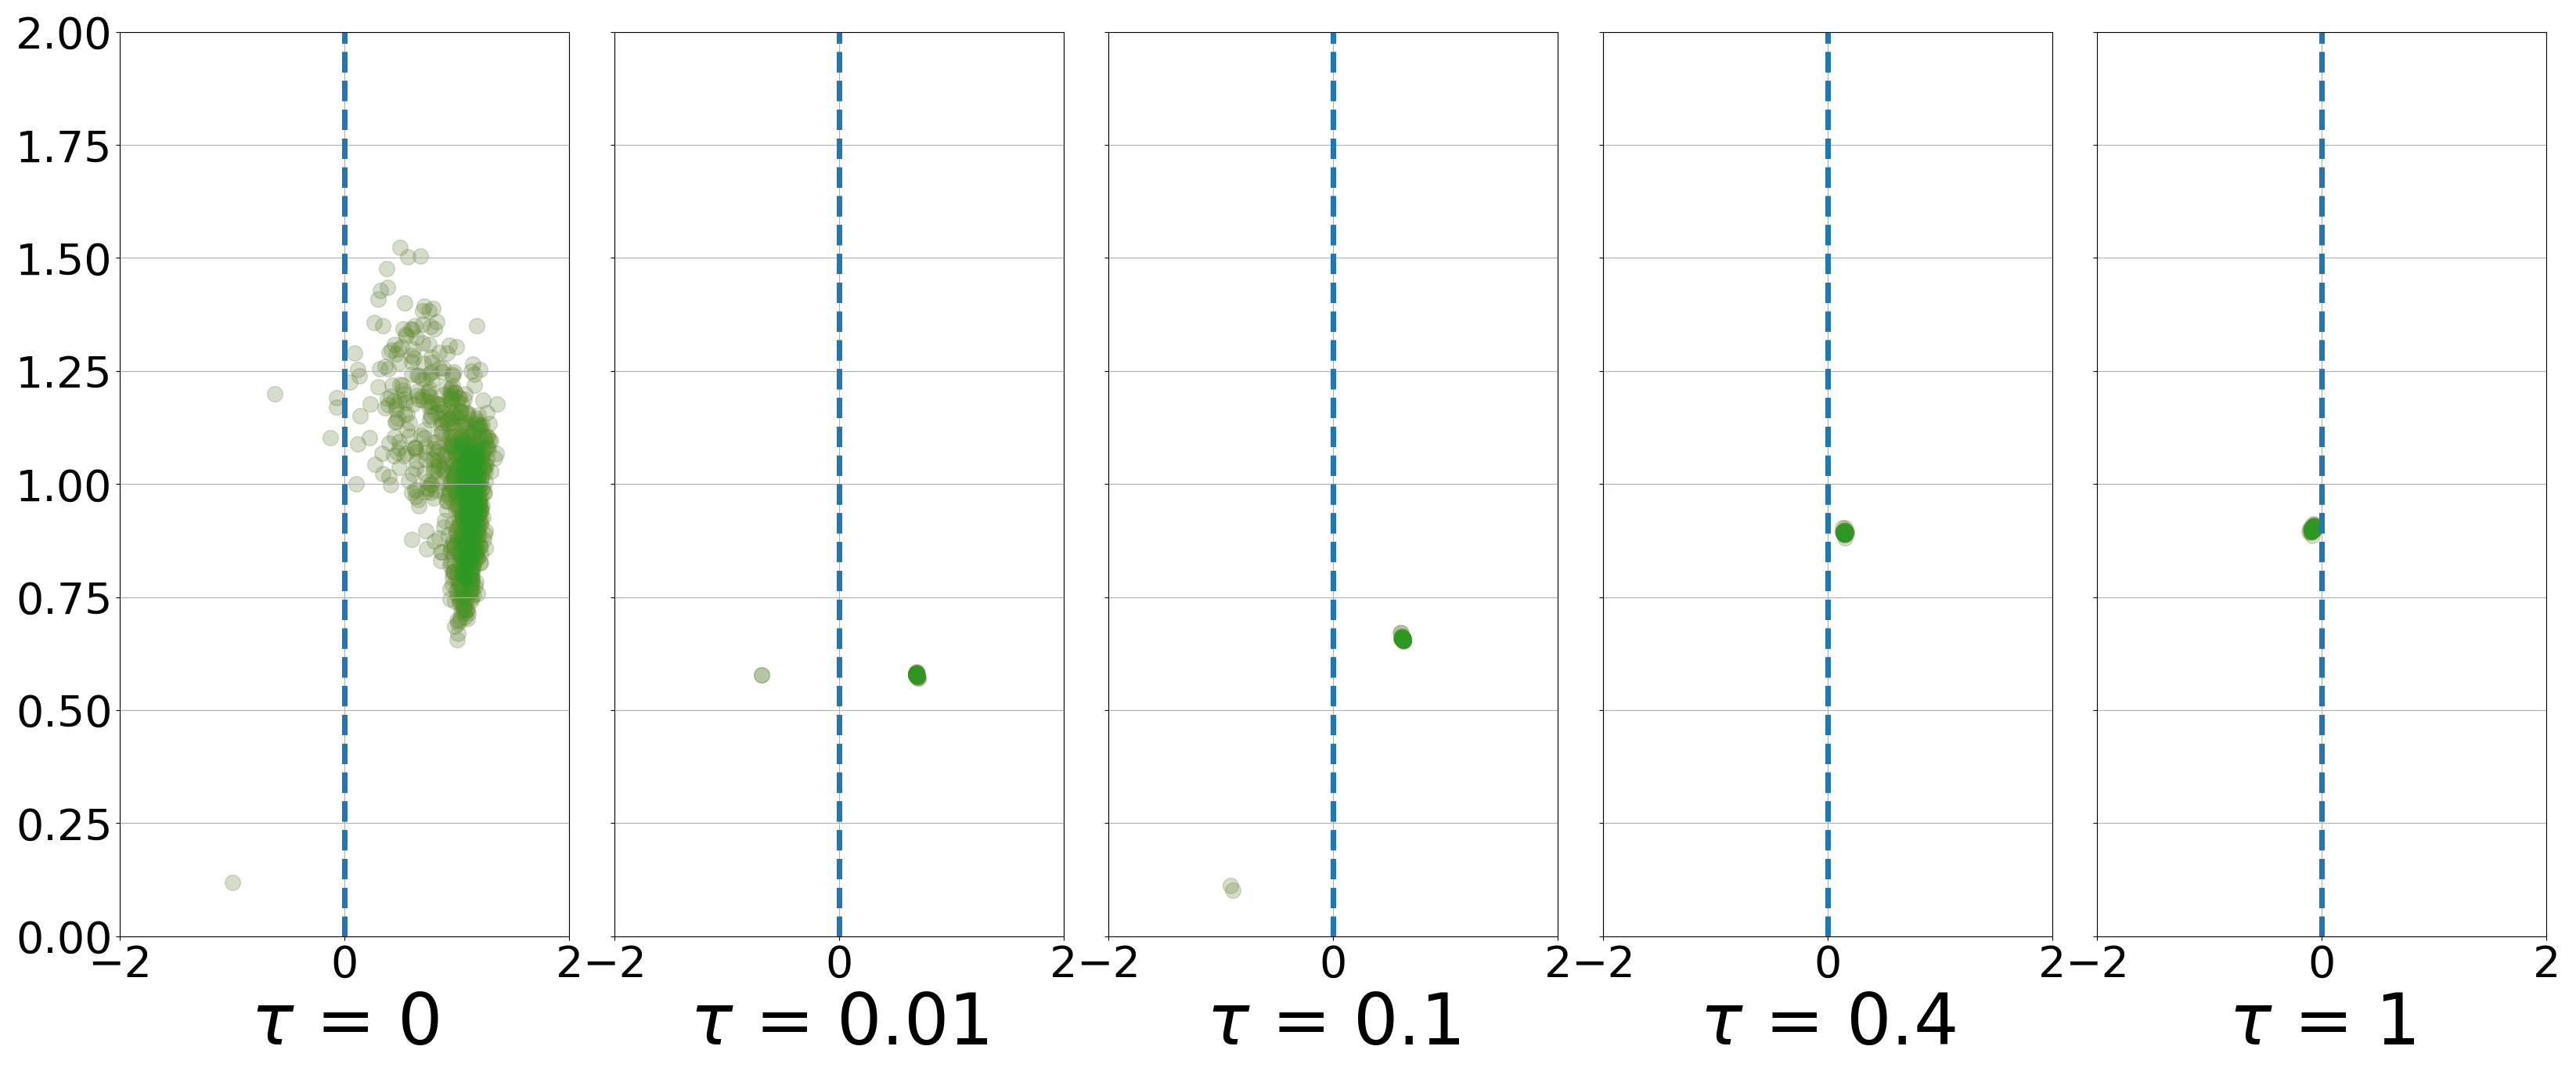
\includegraphics[width=\columnwidth]{figs/continuous-switch-stay/notlearnQ/state0_pi_forward_optim=rmsprop_lr=0.01.png}
    \caption{Forward KL on state 0.}
    \label{fig:cont-switch-stay-forward-s0}
  \end{subfigure}\hspace{15pt}
  
  \begin{subfigure}[b]{0.85\linewidth}
        \centering
        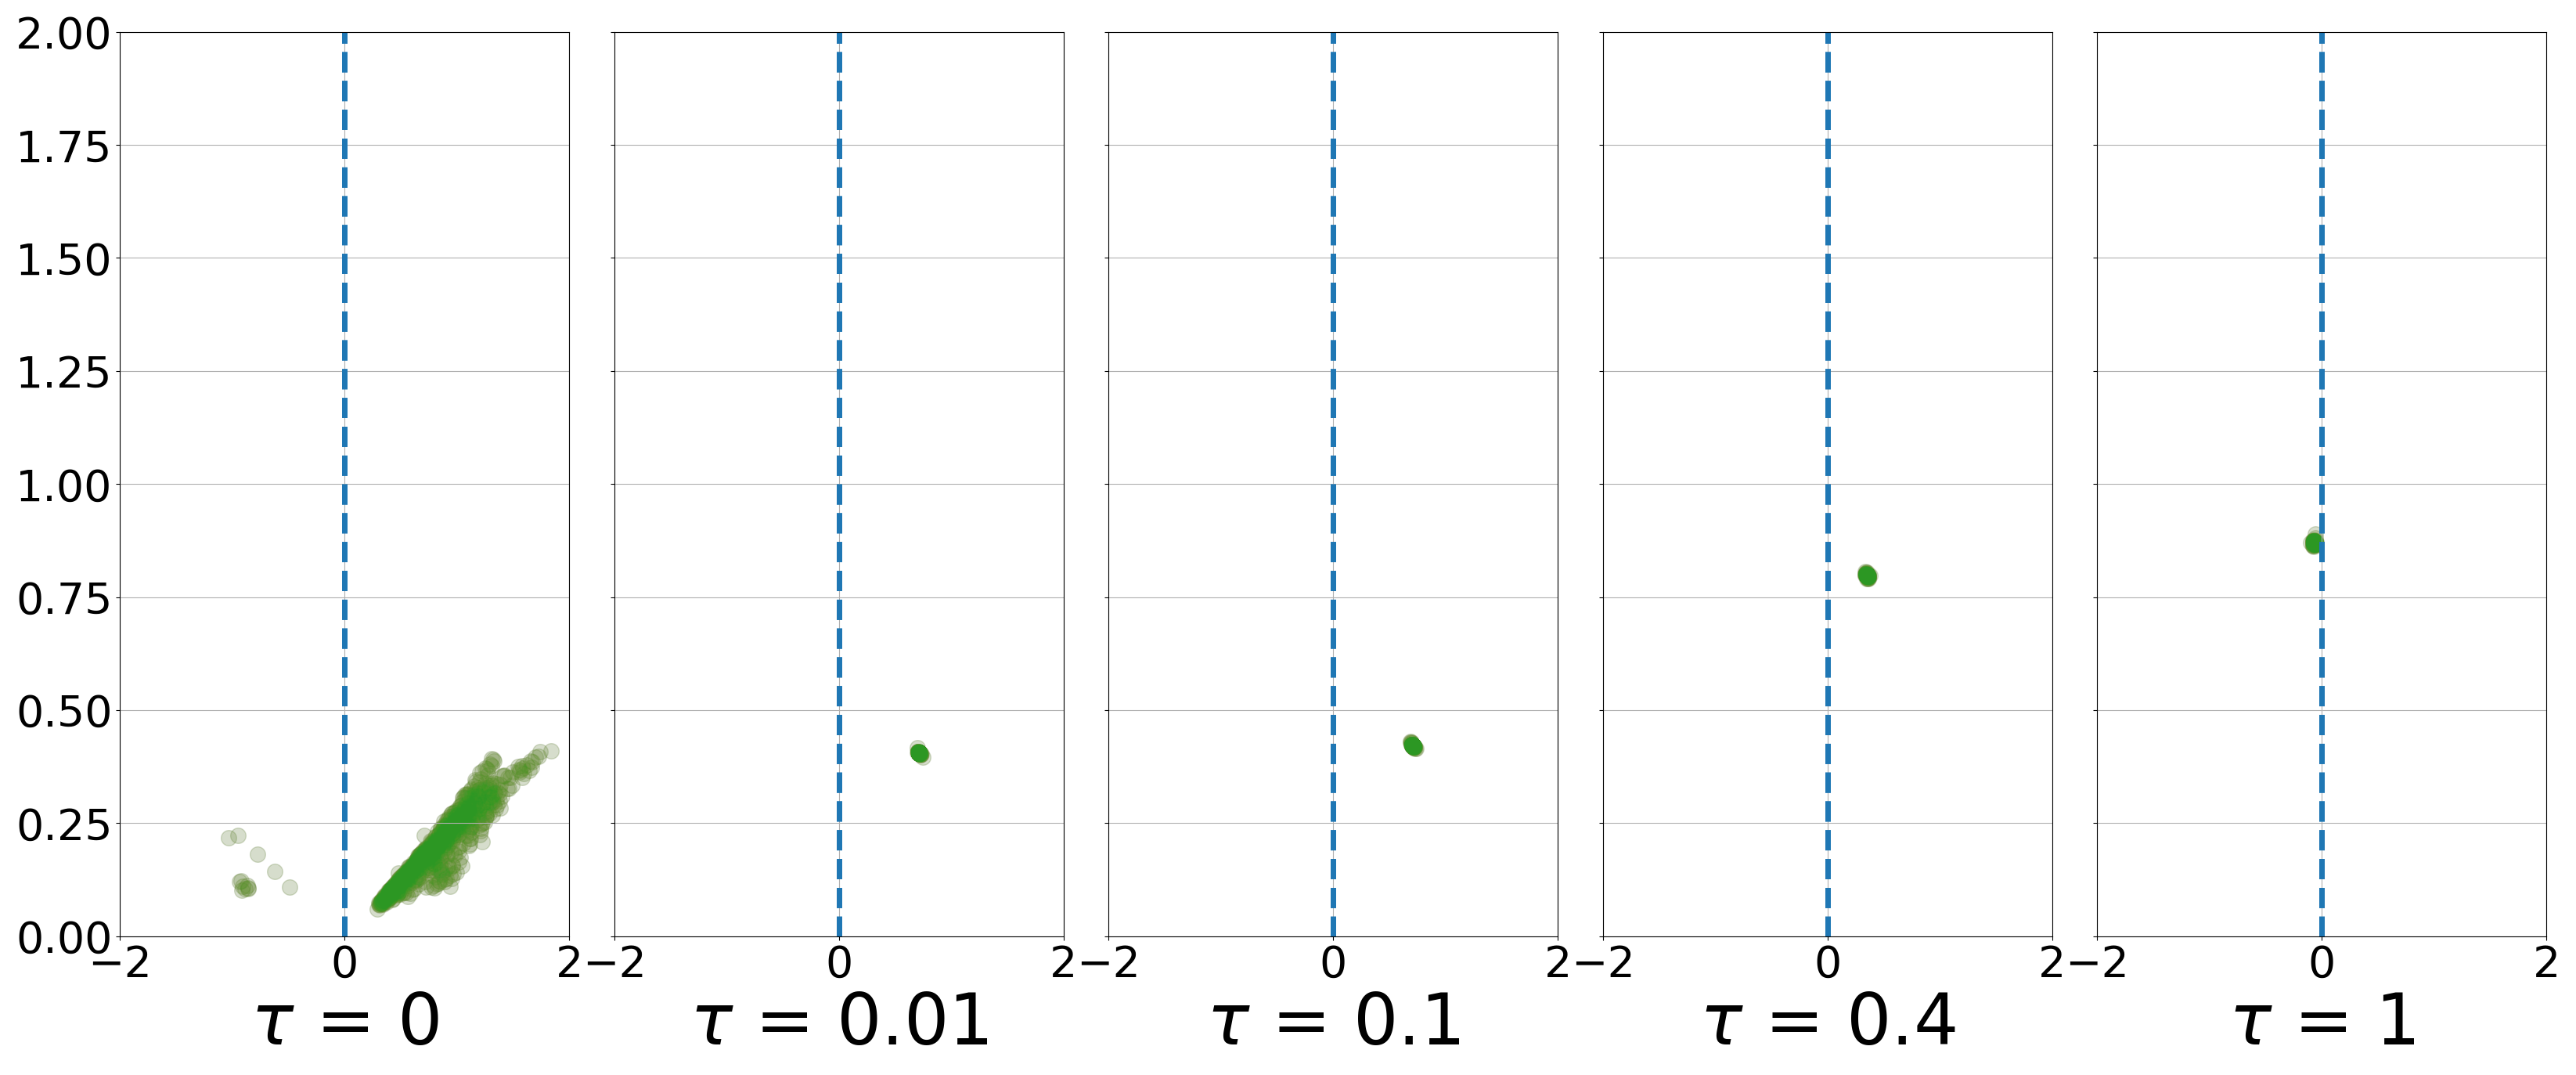
\includegraphics[width=\columnwidth]{figs/continuous-switch-stay/notlearnQ/state0_pi_reverse_optim=rmsprop_lr=0.01.png}
        \caption{Reverse KL on state 0.}
        \label{fig:cont-switch-stay-reverse-s0}
  \end{subfigure}

  \caption{Each subplot plots the final mean (x-axis) and standard deviation (y-axis) on the continuous version of switch-stay after 500 gradient steps with $\gamma = 0.9$ for 1000 iterates. Each iterate is represented by a translucent dot with alpha value $0.1$. Using RMSprop with learning rate $0.01$. Temperature is varied on the $x$-major-axis. Every action $\leq 0$ is treated as ``stay'' and every action $> 0$ is treated as ``switch''. The blue dotted line in subplots corresponds to the line $\mu = 0$. }
  \label{fig:final-ss-probs-0}
\end{figure}


\begin{figure}[!htb]
\centering
\begin{subfigure}[b]{0.85\linewidth}
    \centering
    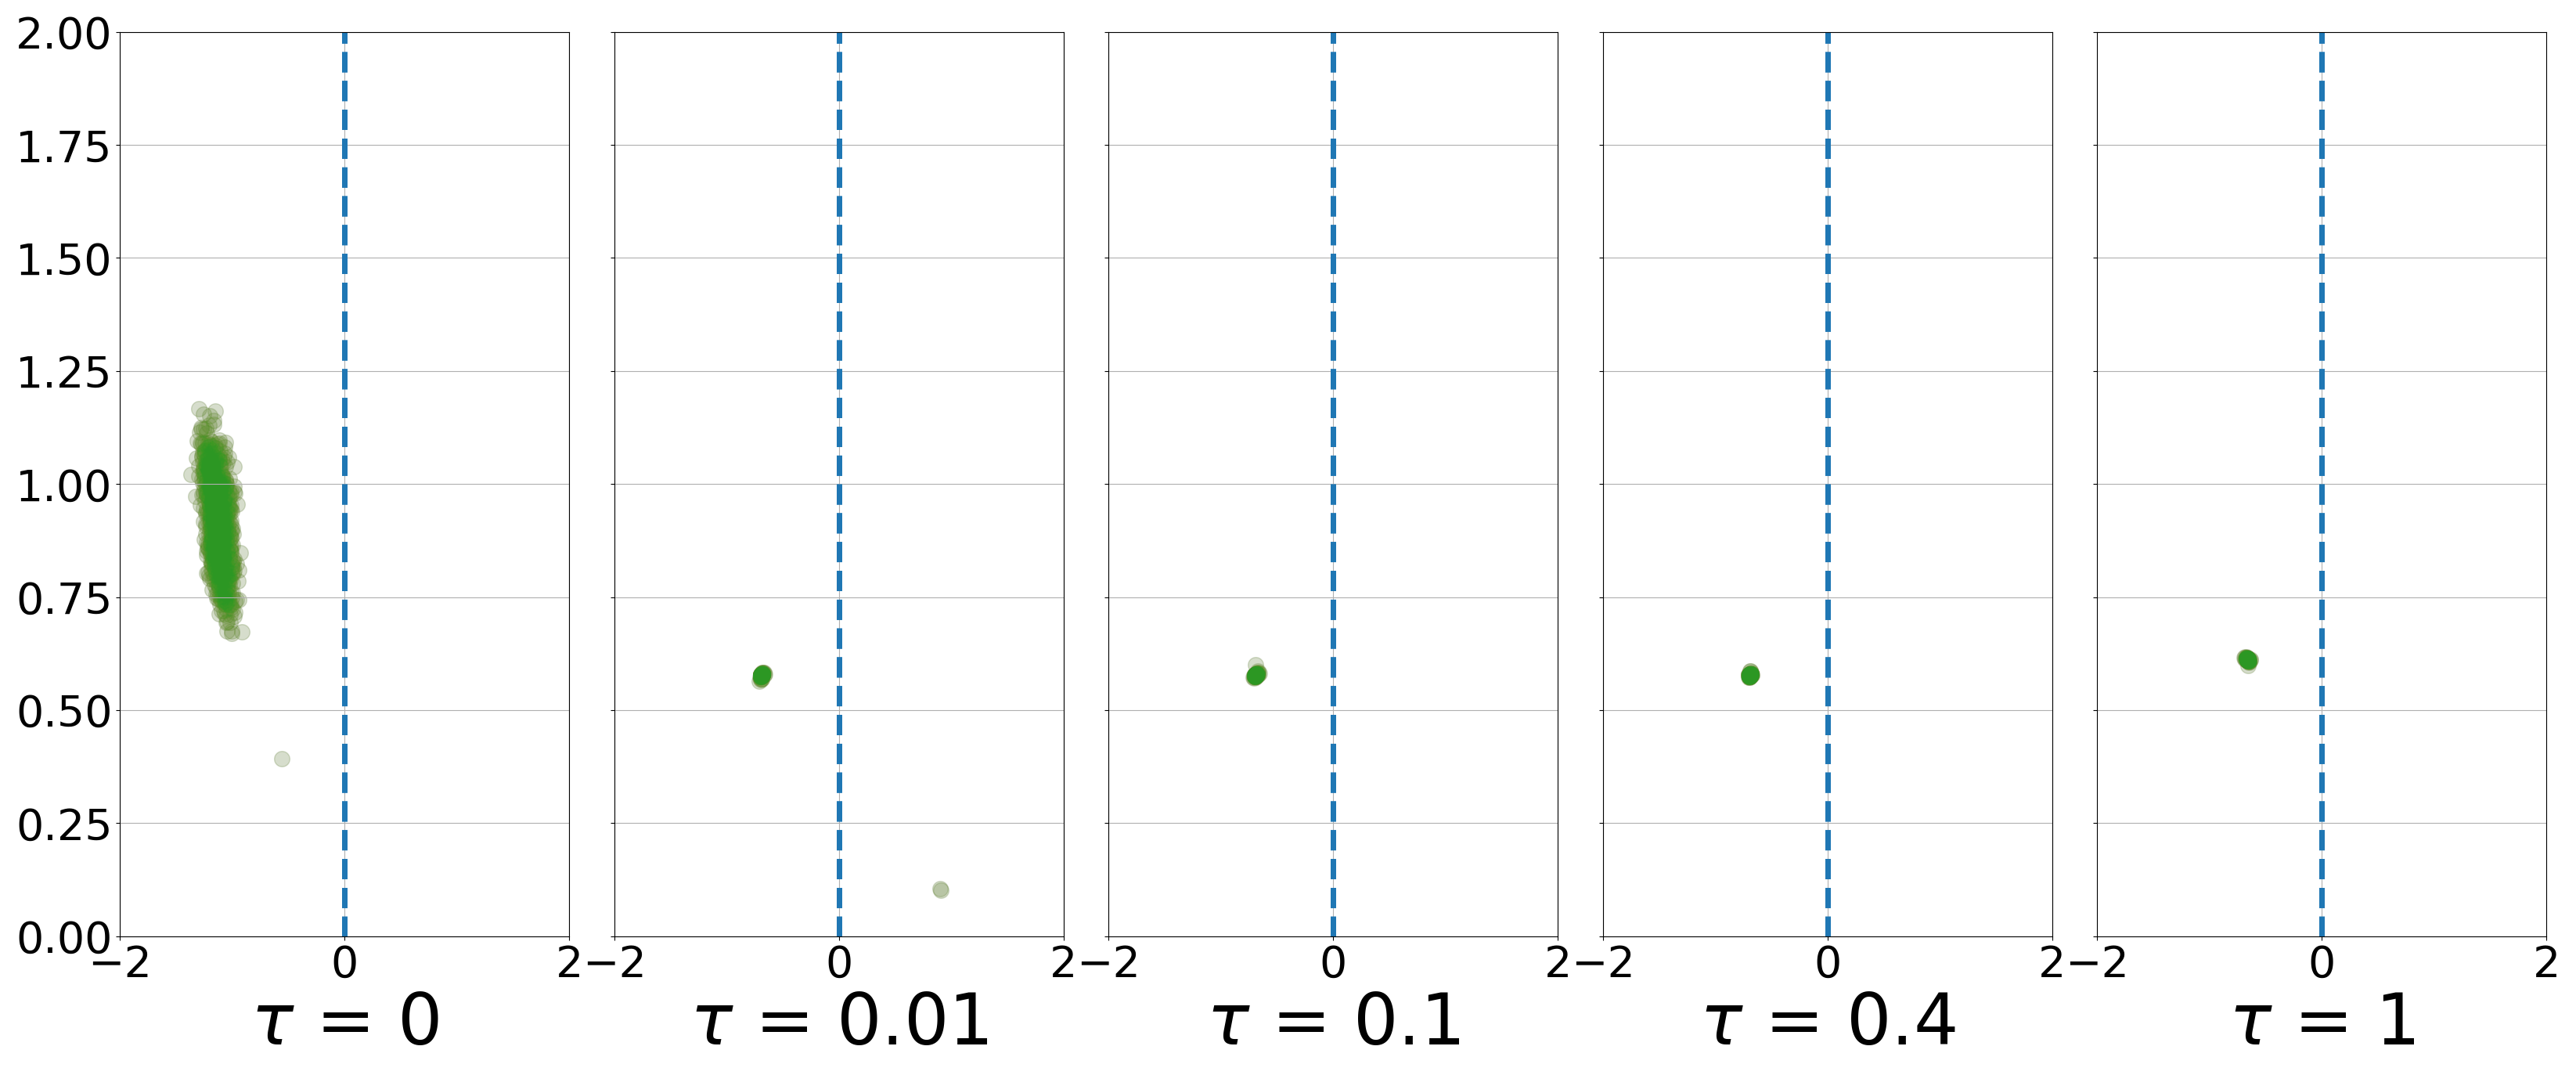
\includegraphics[width=\columnwidth]{figs/continuous-switch-stay/notlearnQ/state1_pi_forward_optim=rmsprop_lr=0.01.png}
    \caption{Forward KL on state 1.}
    \label{fig:cont-switch-stay-forward-s1}
  \end{subfigure}\hspace{15pt}
  
  \begin{subfigure}[b]{0.85\linewidth}
        \centering
        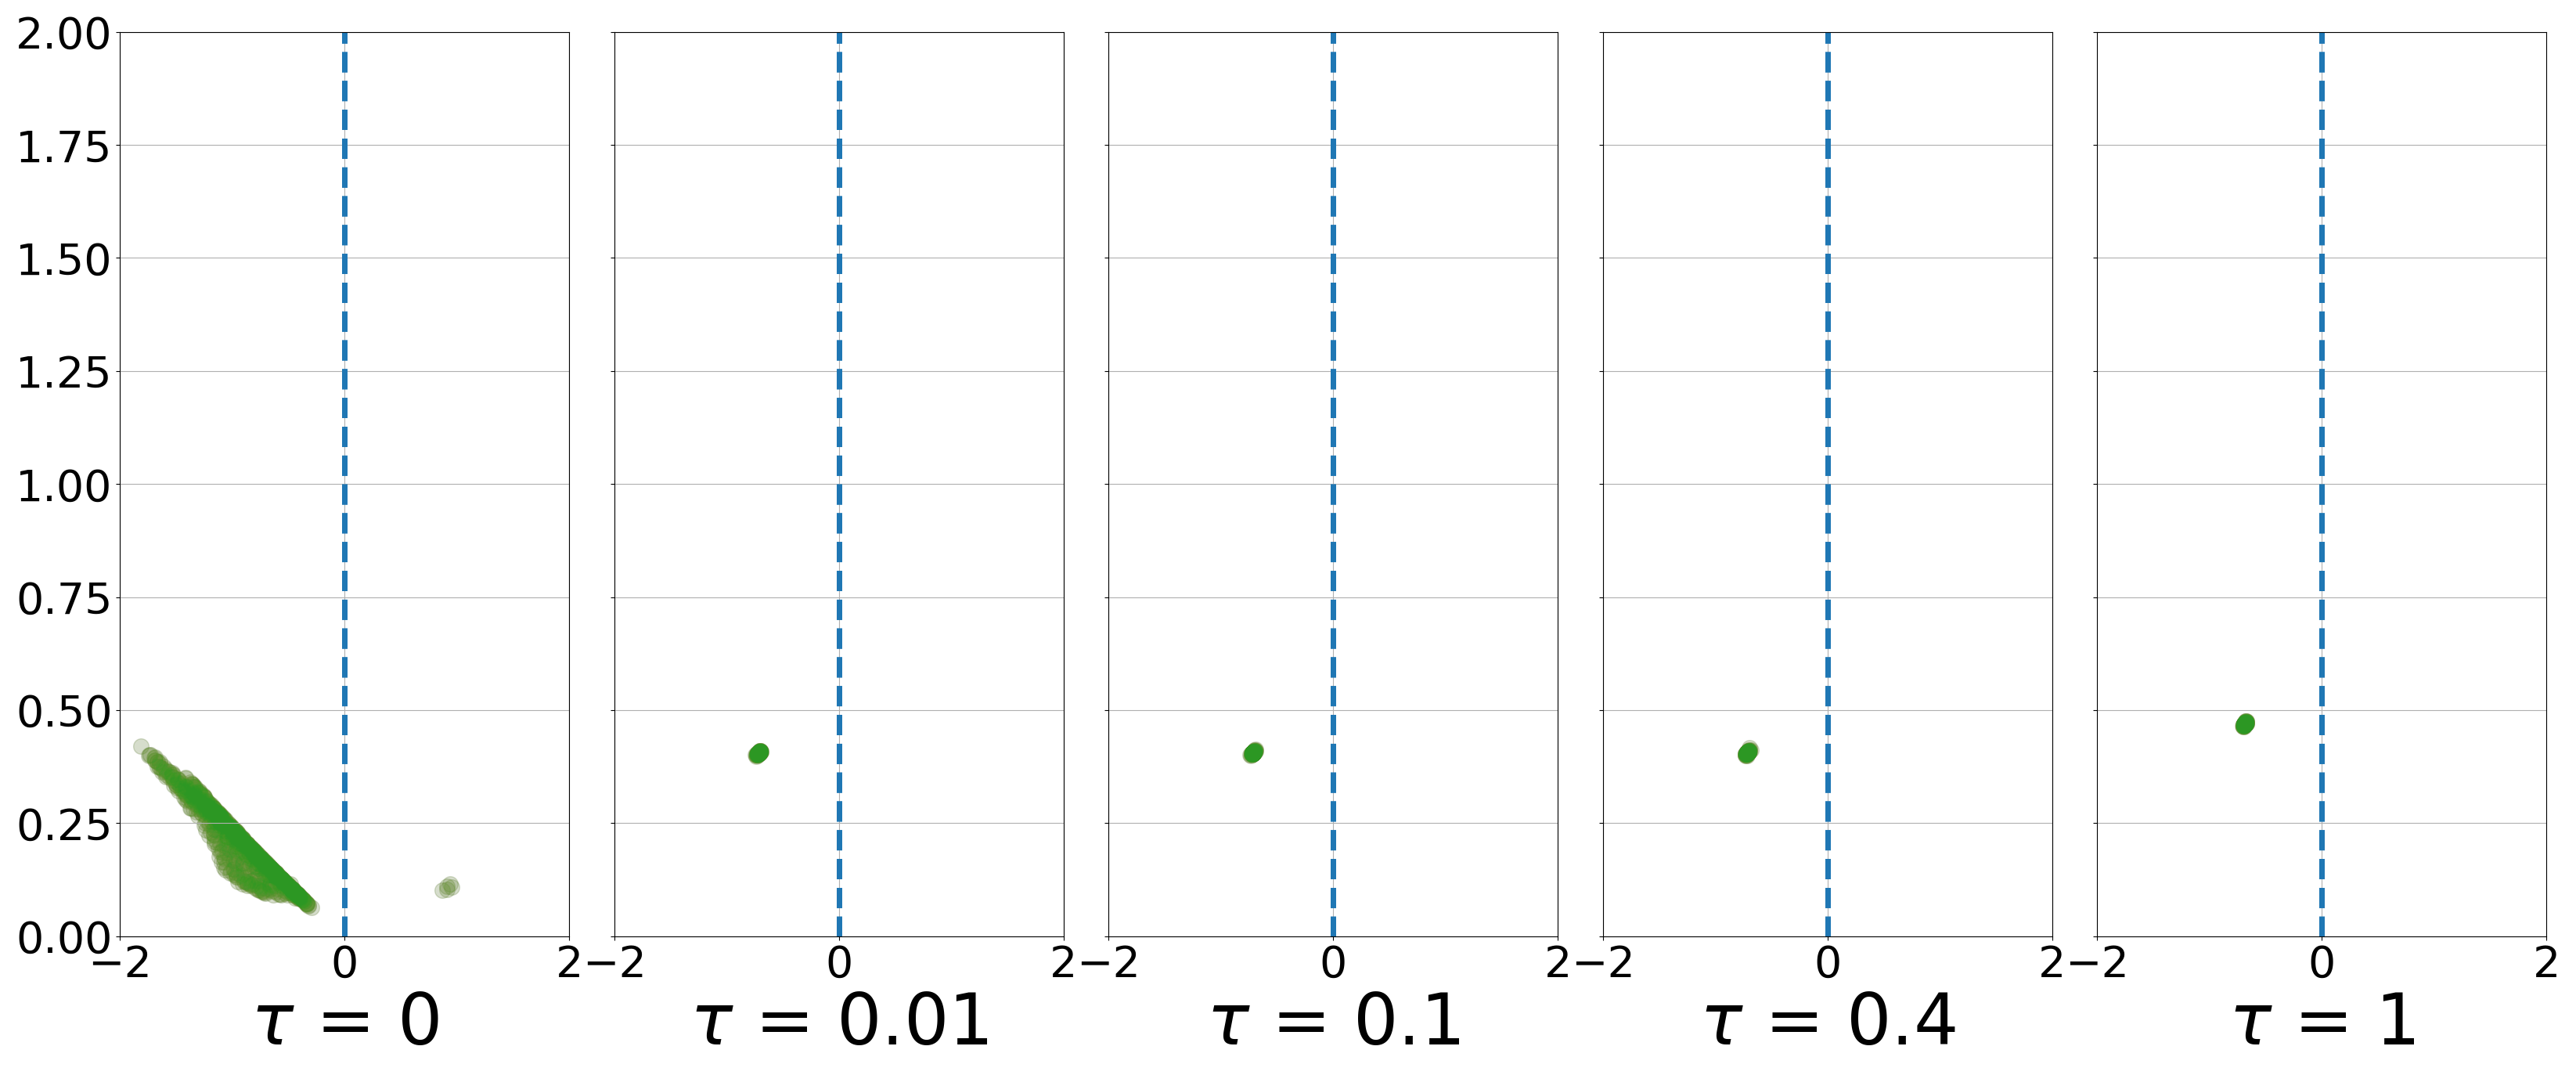
\includegraphics[width=\columnwidth]{figs/continuous-switch-stay/notlearnQ/state1_pi_reverse_optim=rmsprop_lr=0.01.png}
        \caption{Reverse KL on state 1.}
        \label{fig:cont-switch-stay-reverse-s1}
  \end{subfigure}
  \caption{See \Cref{fig:final-ss-probs-0}.}
  \label{fig:final-ss-probs-1}
\end{figure}

We also note here that when fewer integration points were used in an earlier version of this experiment, RKL exhibited substantial instability and a large number of iterates across temperatures and $\sigma_0$ values converged to suboptimal deterministic policies. This phenomenon might be related to the effect of stochasticity when approximating the KL loss, which is discussed in \Cref{sec:stochastic-microworld}.

 
\subsection{Discrete-Action Results}\label{sec:microworld-discrete-actions}

Overall, there is markedly less distinction between RKL and FKL in the discrete action setting with a softmax policy parameterization. In the heatmap in \Cref{fig:discrete-heatmap}, the loss surfaces for both KLs are very similar for a given temperature, in contrast to the heatmap for the continuous bandit. As the temperature increases, the black region (region with low loss) moves closer to the middle of the plot, which is consistent with the fact that the target distribution becomes closer to uniform as the temperature increases. 
\begin{figure}[!htb]
    \centering
    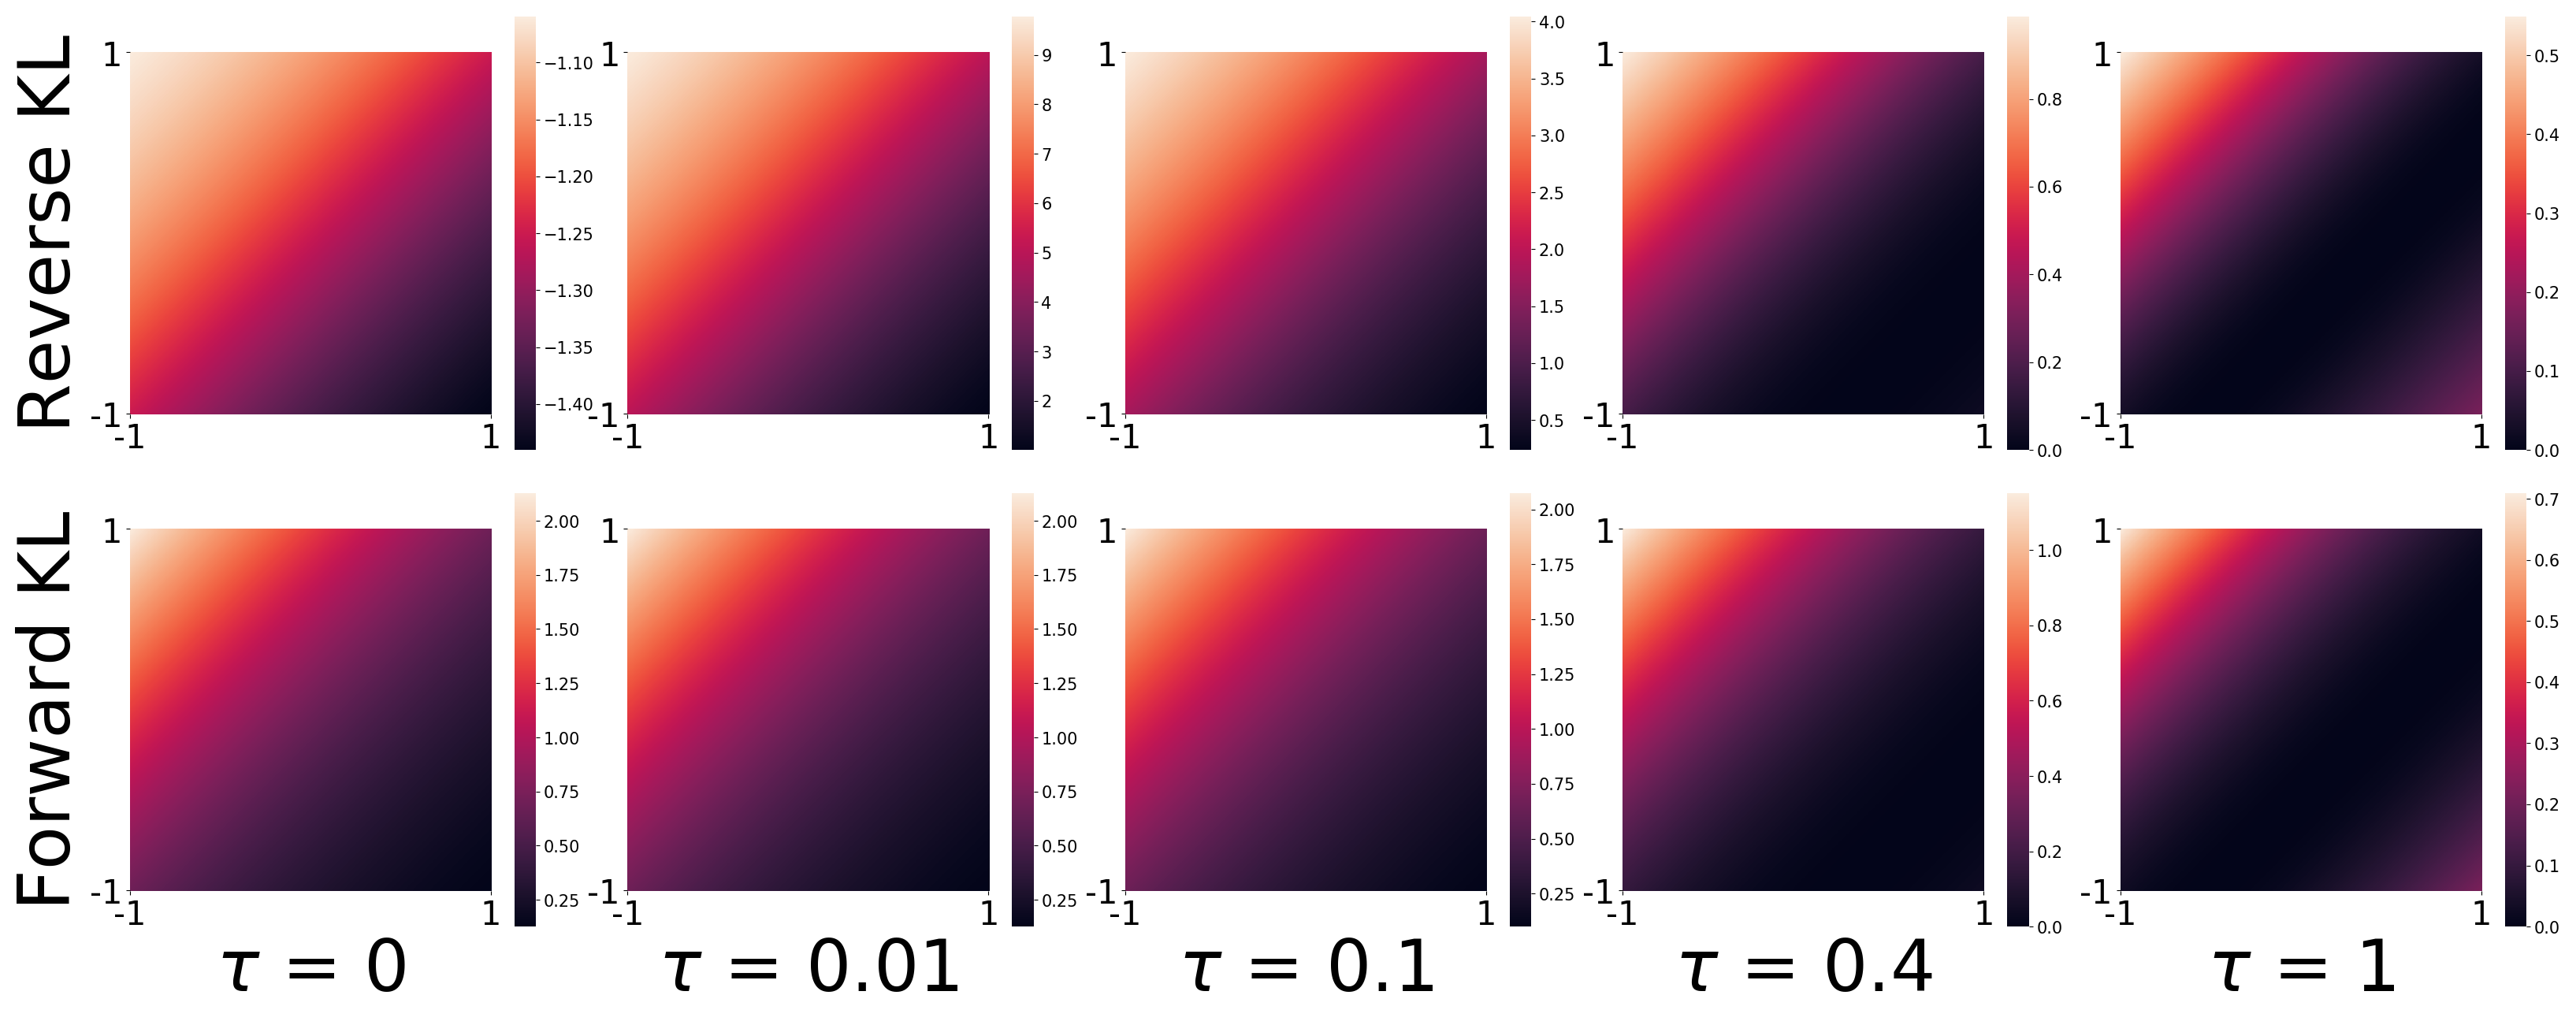
\includegraphics[width=1\columnwidth]{figs/discrete-bandit/heatmaps/discrete.png}
    \caption{Heatmap for the KLs on the discrete bandit. In a given subplot, the $x$-axis is the logit for the optimal arm and the $y$-axis is the logit for the suboptimal arm.}
    \label{fig:discrete-heatmap}
  \end{figure}

Next, we track the progress of 1000 iterates over 1000 gradient steps. For each iterate, we initialize each logit--one for each arm--uniformly in $(-1, 1)$. The behaviour policy is thus the result of the softmax function applied to the logit vector. 

When looking at 1000 iterates over 1000 gradient steps, both RKL and FKL iterates learn the optimal arms in \Cref{fig:discrete-bandit-prob-forward-rmsprop,fig:discrete-bandit-prob-reverse-rmsprop}. There is little difference in the behaviour of iterates under either KL; there seems just to be one global optimum to which iterates under either KL converge reliably. 

% \begin{figure}[!htb]
%   \centering
%   \begin{subfigure}[b]{1\linewidth}
%     \centering
%     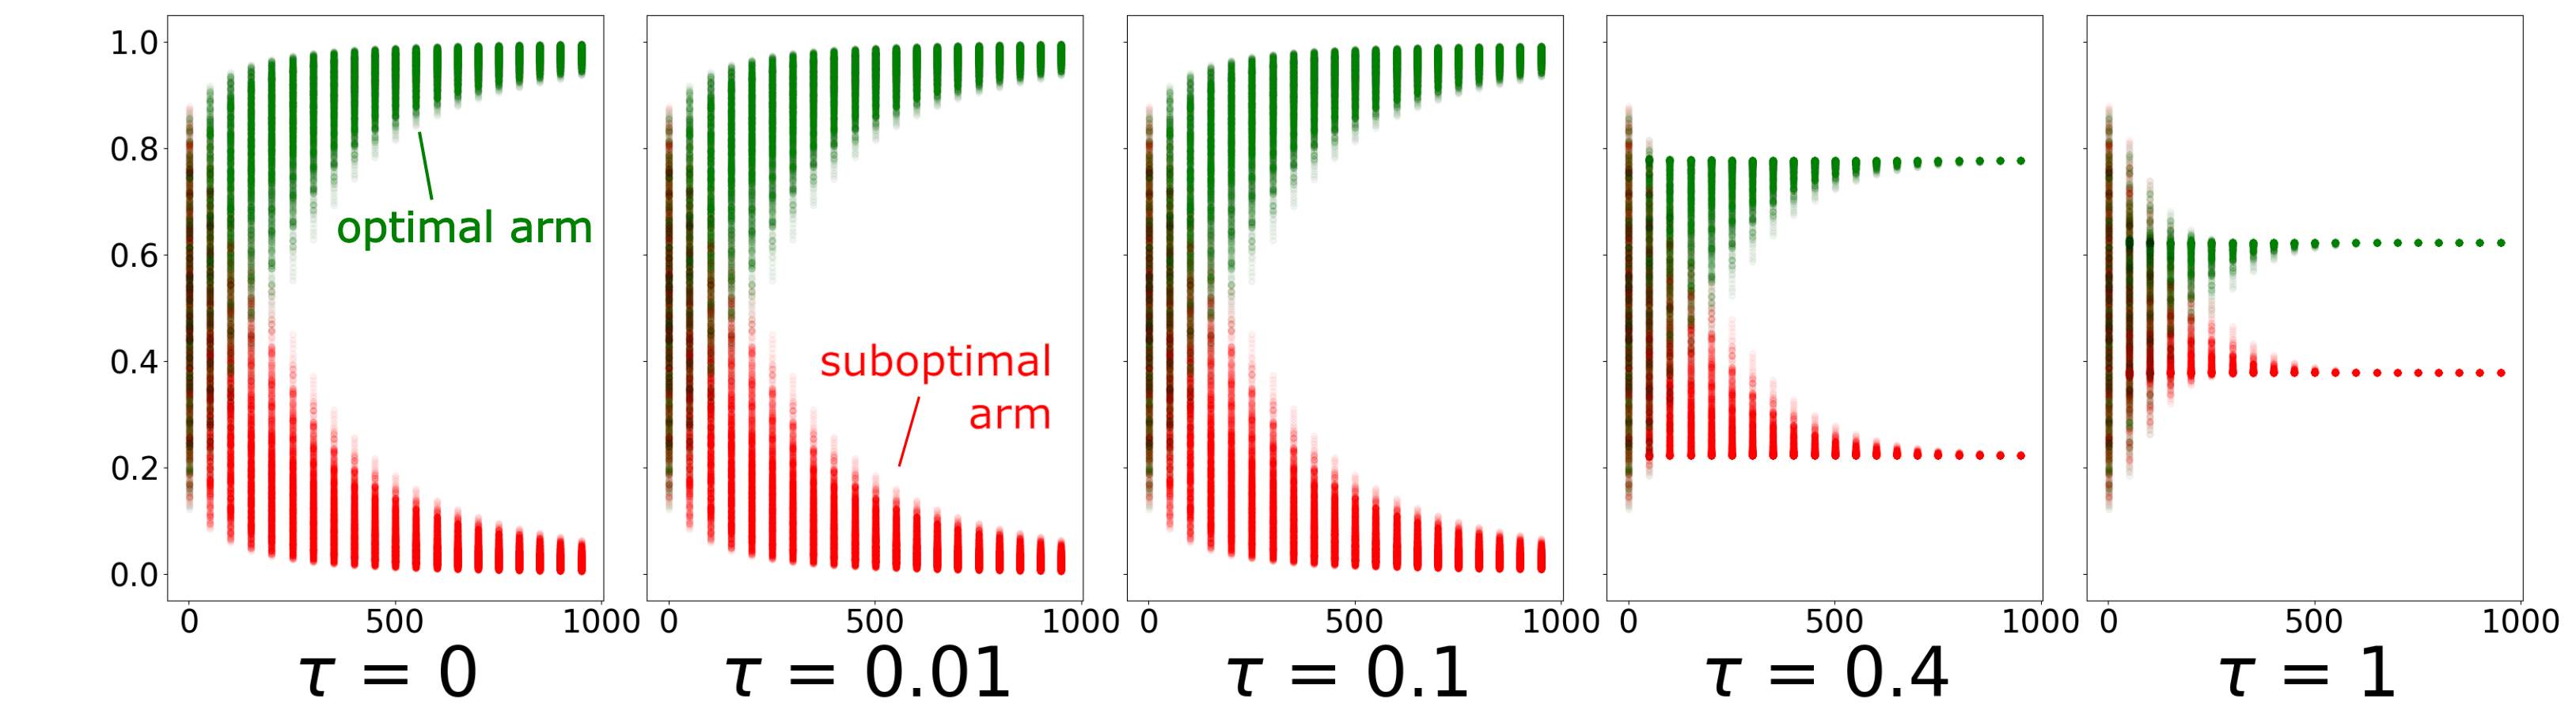
\includegraphics[width=1\columnwidth]{figs/discrete-bandit/notlearnQ/adam/prob-adam.png}
%     \caption{Forward KL, Adam.}
%     \label{fig:discrete-bandit-prob-forward-adam}
%   \end{subfigure}%
  
%   \begin{subfigure}[b]{1\linewidth}
%     \centering
%     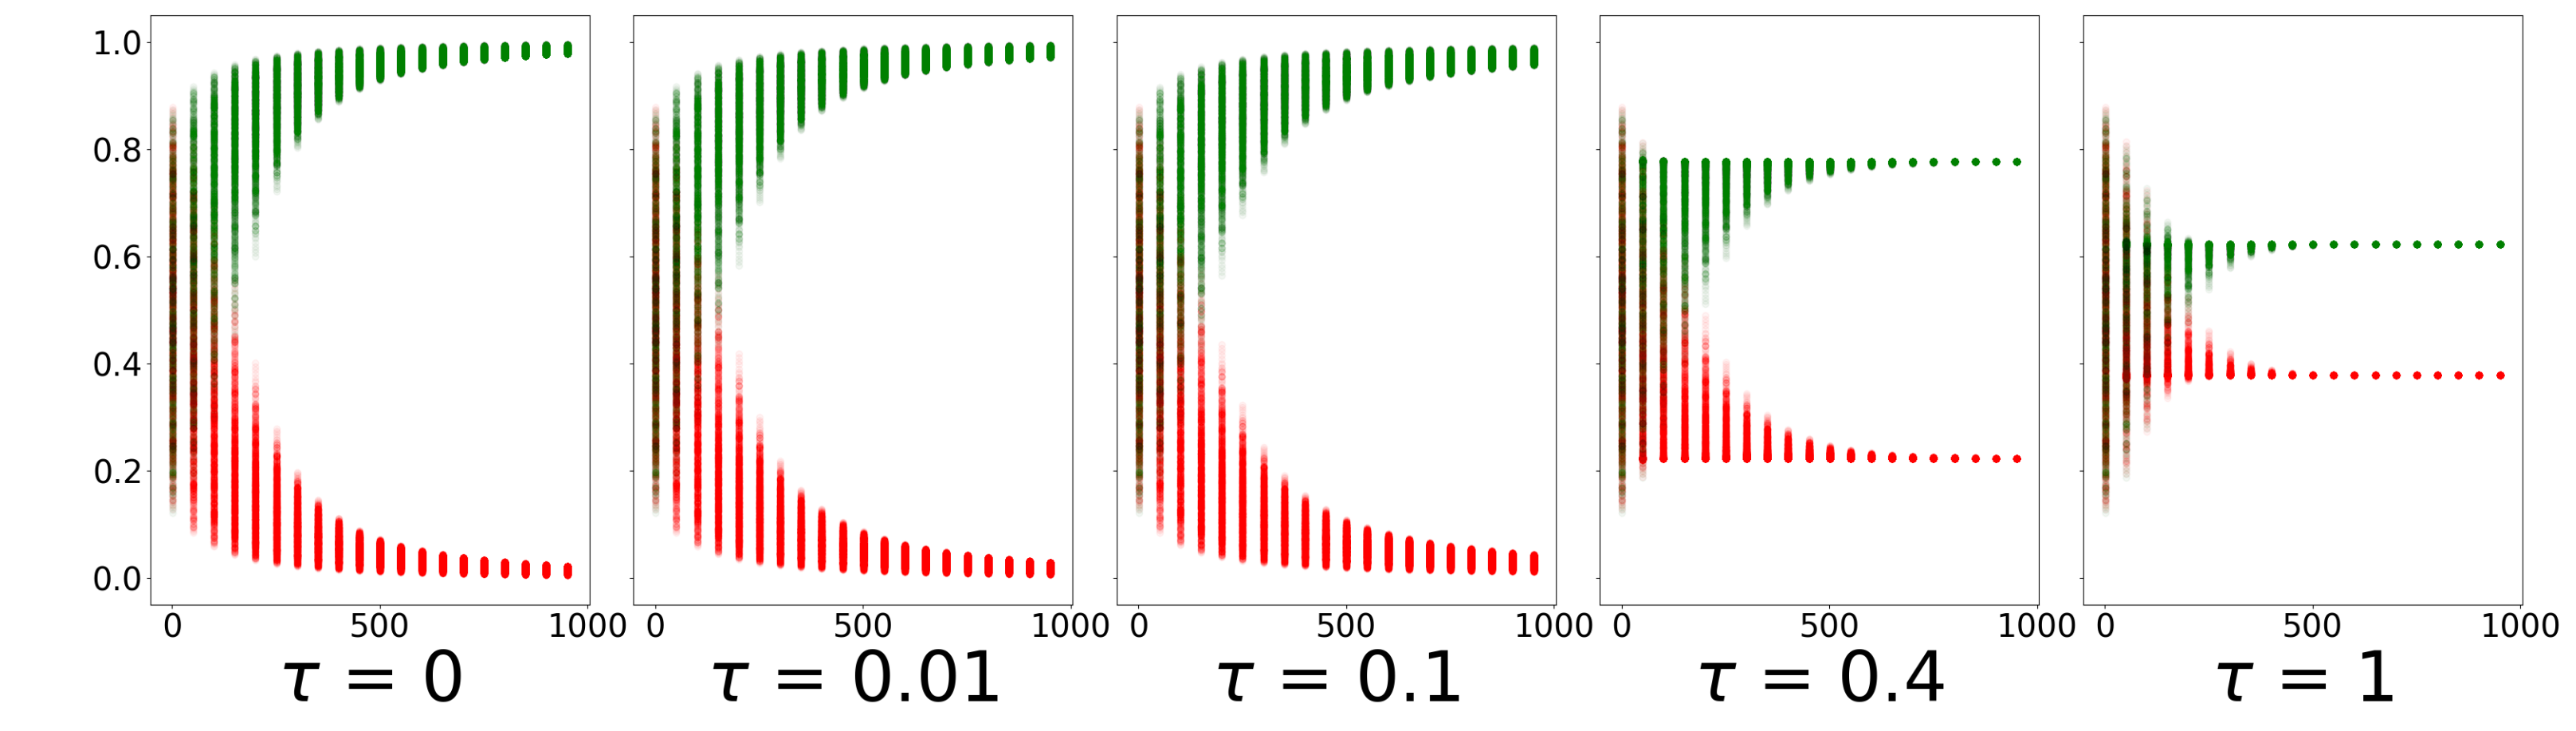
\includegraphics[width=1\columnwidth]{figs/discrete-bandit/notlearnQ/adam/prob-reverse-adam.png}
%     \caption{Reverse KL, Adam. }
%     \label{fig:discrete-bandit-prob-reverse-adam}
%   \end{subfigure}
%   \caption{Each subplot tracks the learned probability of each arm for 1000 iterates over 1000 gradient steps. The learning rate is set to be 0.005 and Adam is the optimizer. }
% \end{figure}

\begin{figure}[!htb]
  \centering
  \begin{subfigure}[b]{1\linewidth}
    \centering
    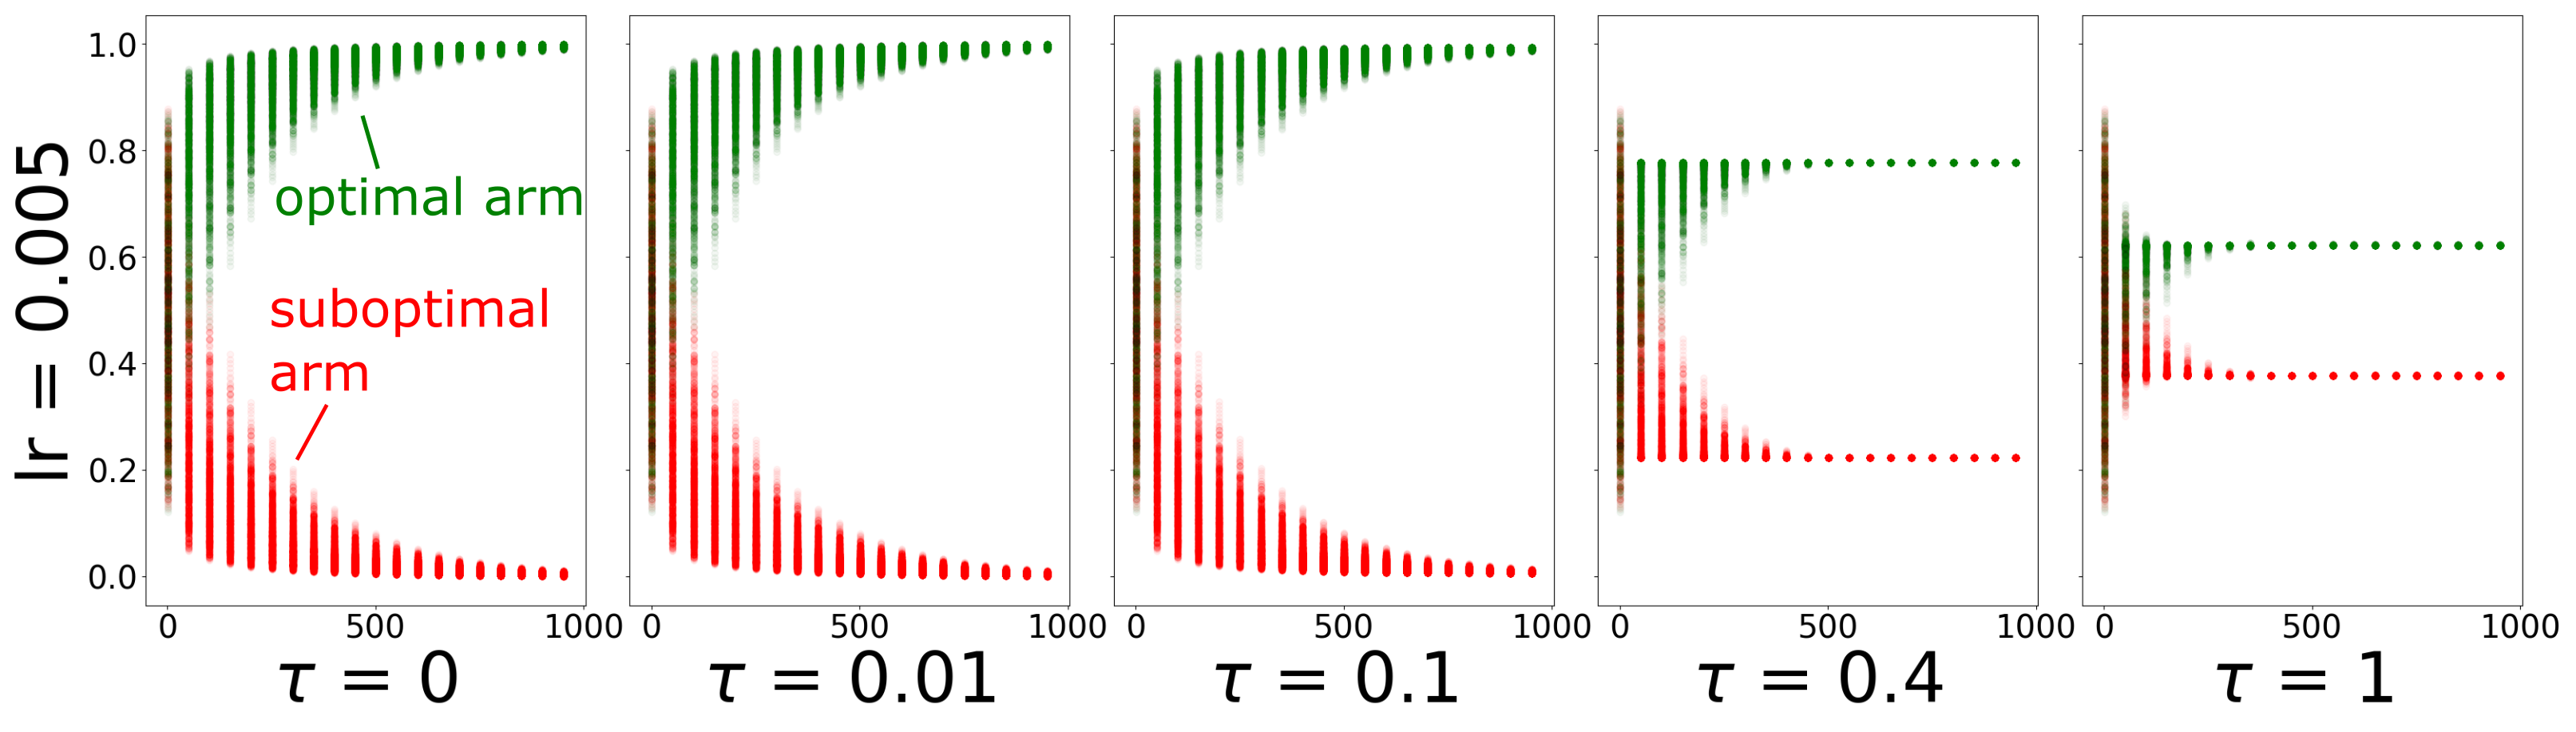
\includegraphics[width=1\columnwidth]{figs/discrete-bandit/notlearnQ/rmsprop/prob_forward_optim=rmsprop_lr=0.005.png}
    \caption{Forward KL.}
    \label{fig:discrete-bandit-prob-forward-rmsprop}
  \end{subfigure}%
  
  \begin{subfigure}[b]{1\linewidth}
    \centering
    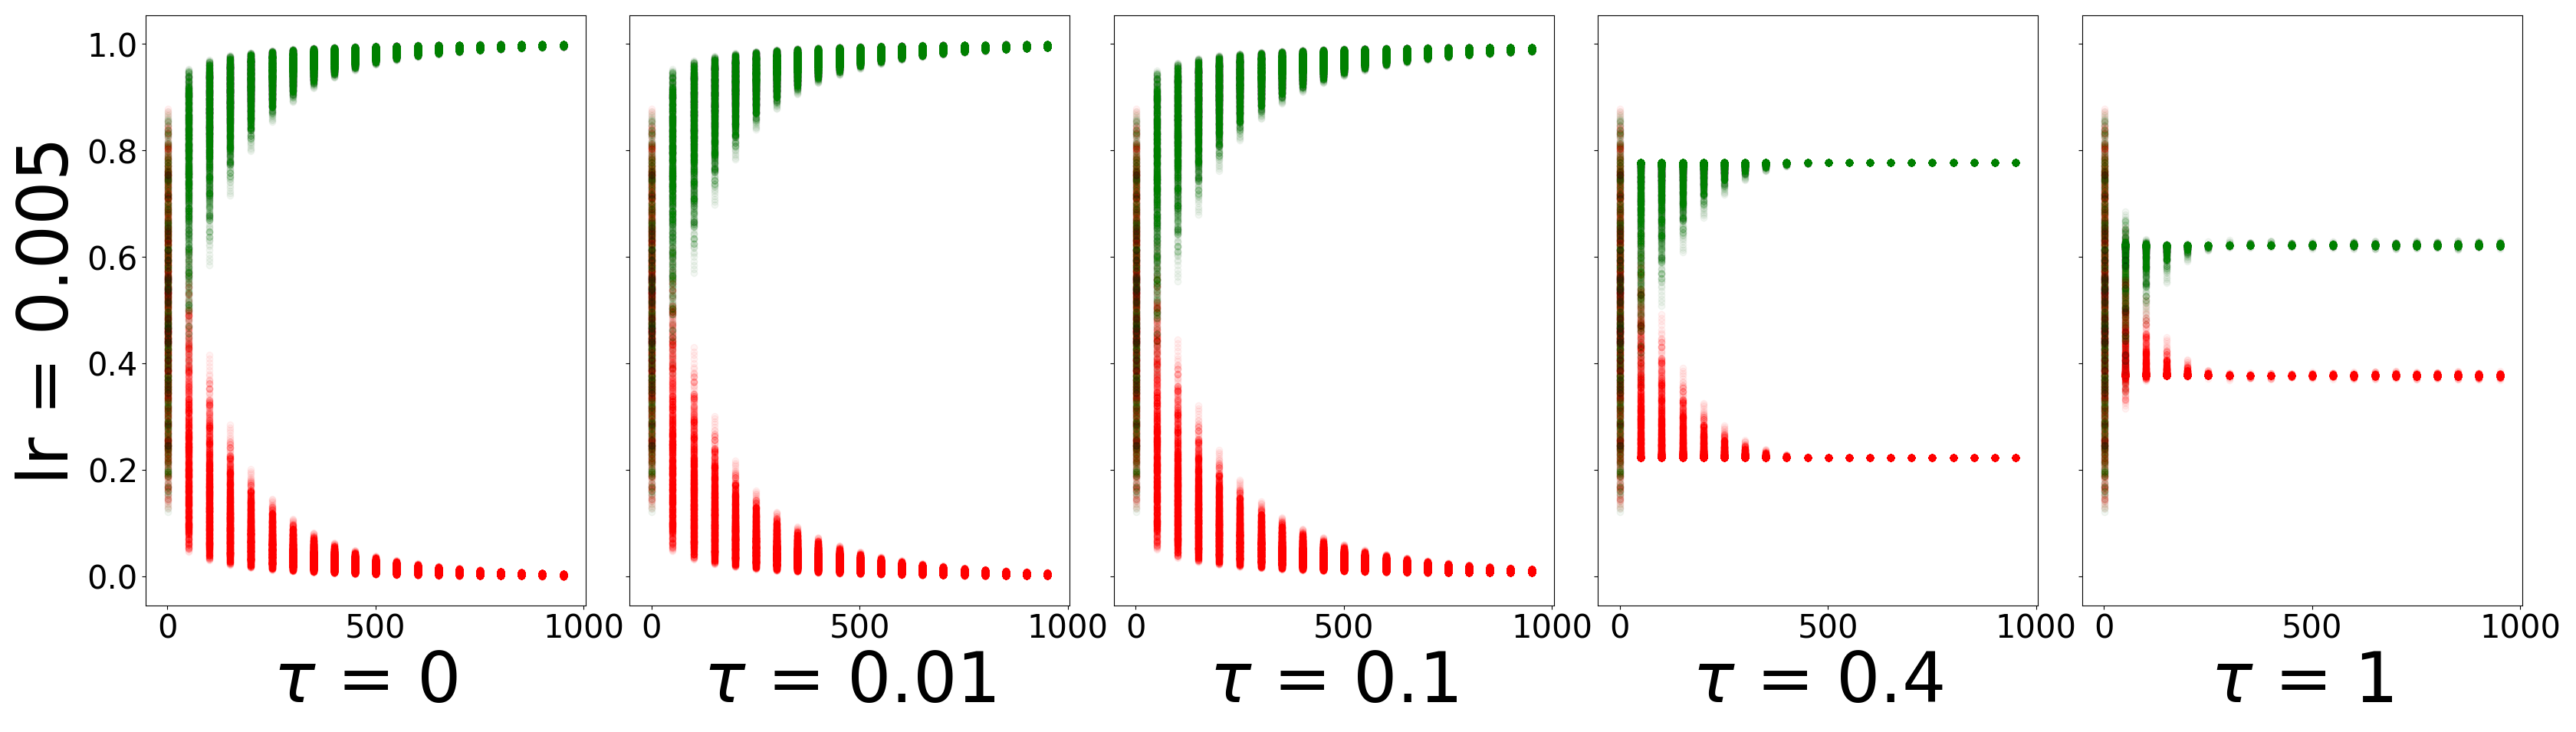
\includegraphics[width=1\columnwidth]{figs/discrete-bandit/notlearnQ/rmsprop/prob_reverse_optim=rmsprop_lr=0.005.png}
    \caption{Reverse KL. }
    \label{fig:discrete-bandit-prob-reverse-rmsprop}
  \end{subfigure}
  \caption{Each subplot tracks the learned probability of each arm for 1000 iterates over 1000 gradient steps. The learning rate is set to be 0.005. }
\end{figure}


Results for discrete Switch-Stay are in \Cref{fig:discrete-ss-all}. Both FKL and RKL iterates move in the direction of the optimal value function, but RKL iterates seem to converge faster. While a difference in convergence speed did also exist on the continuous version of Switch-Stay, the distinction is less notable here. 

For higher temperatures, the limit point of the iterates is slightly further away from the optimal value function of the original MDP than for lower temperatures. This result is to be expected given that in general, the optimal entropy-regularized policy is different from the optimal non-regularized policy \citep{geist2019theory}.

% \begin{figure}[!htb]
%   \centering
%   \begin{subfigure}[b]{0.5\linewidth}
%     \centering
%     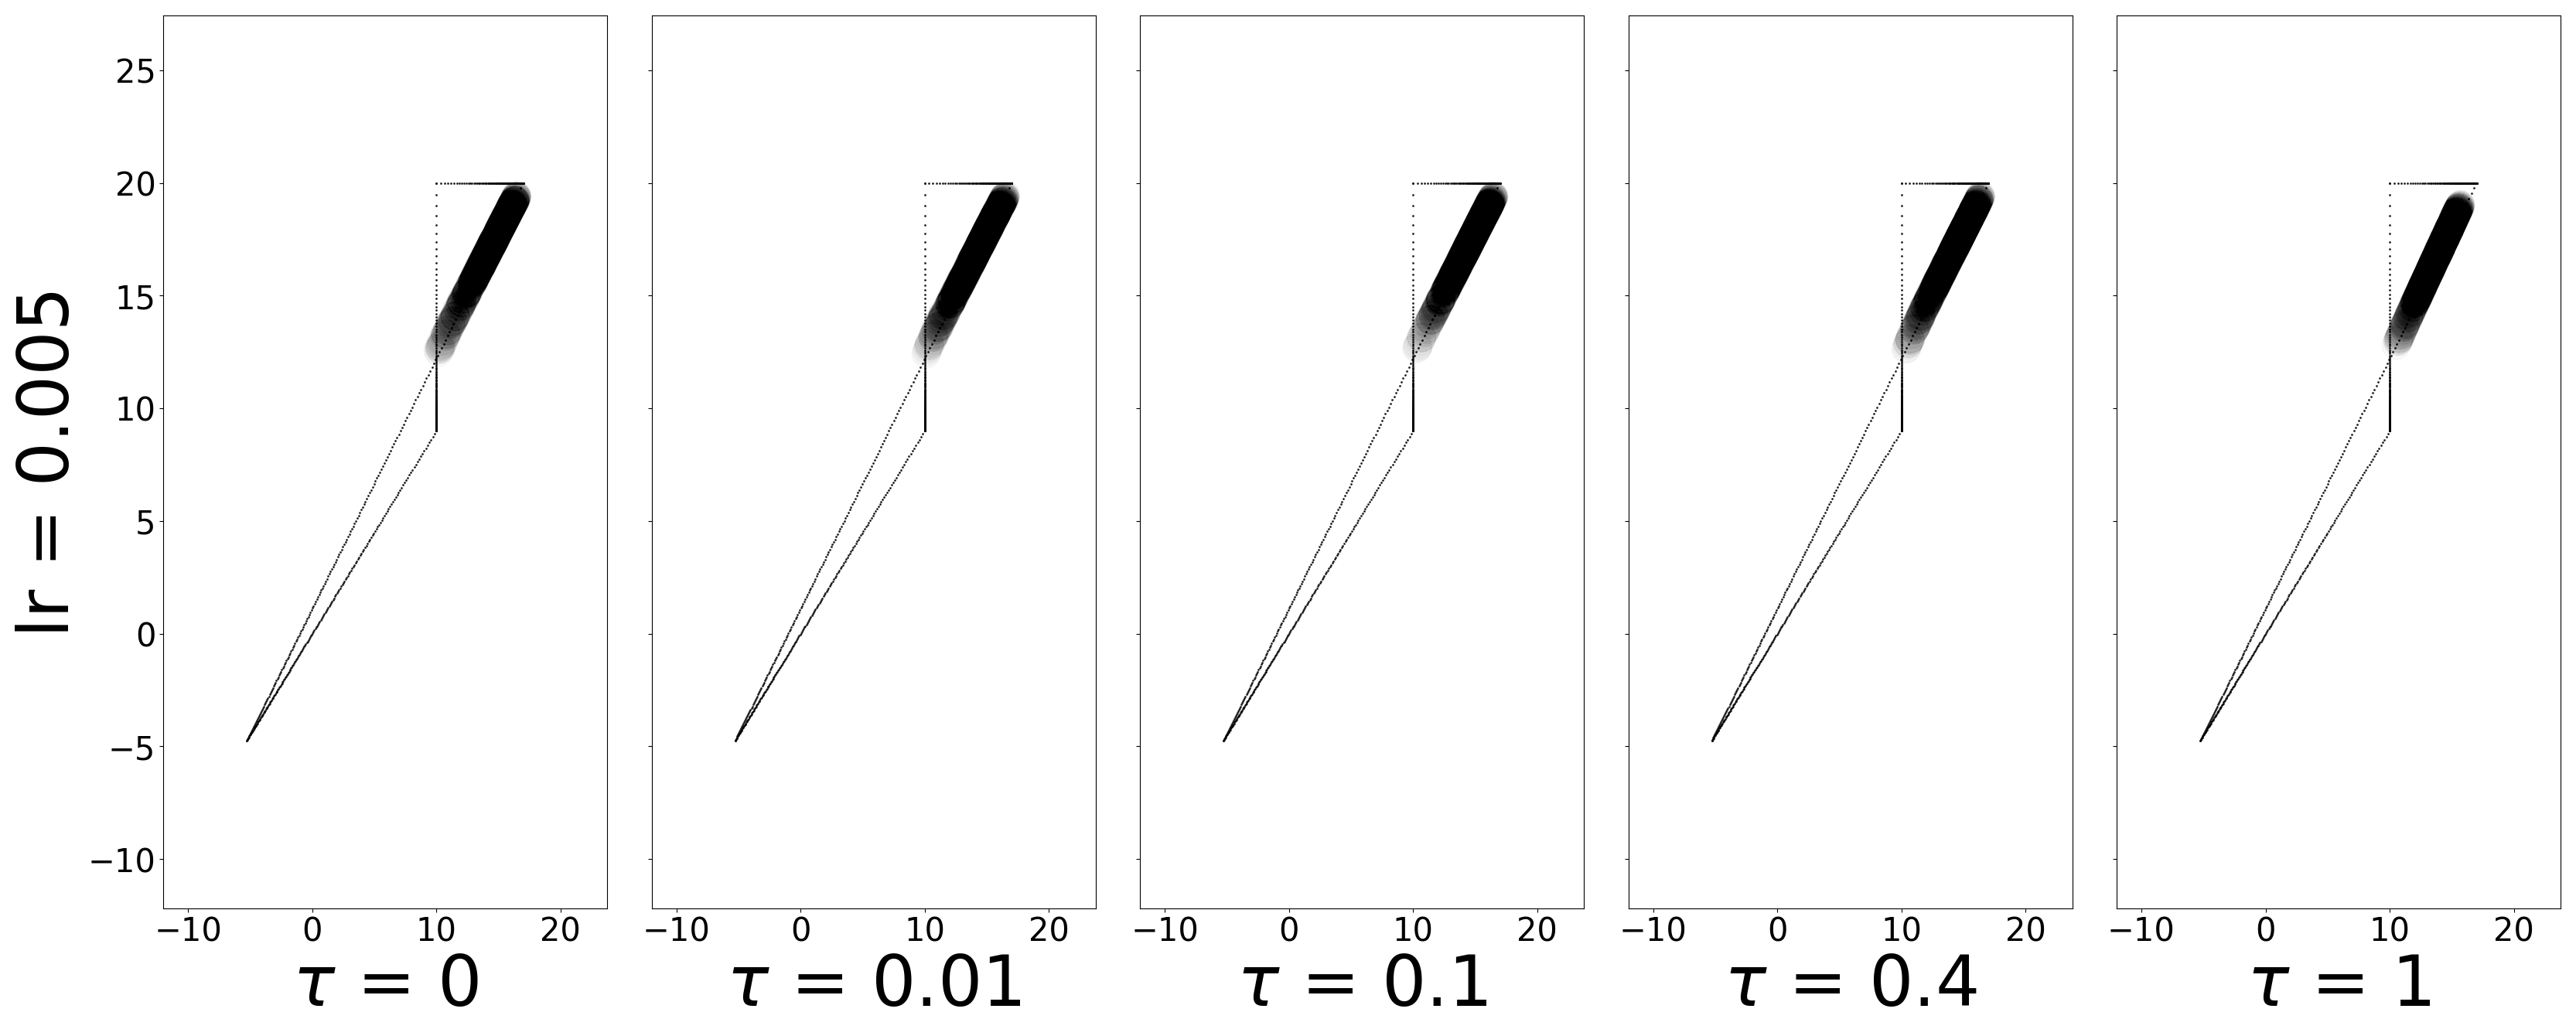
\includegraphics[width=0.8\columnwidth]{figs/switch-stay/notlearnQ/polytope_forward_optim=adam.png}
%     \caption{Forward KL.}
%     \label{fig:discrete-switch-stay-forward-adam}
%   \end{subfigure}%
%   \begin{subfigure}[b]{0.5\linewidth}
%         \centering
%         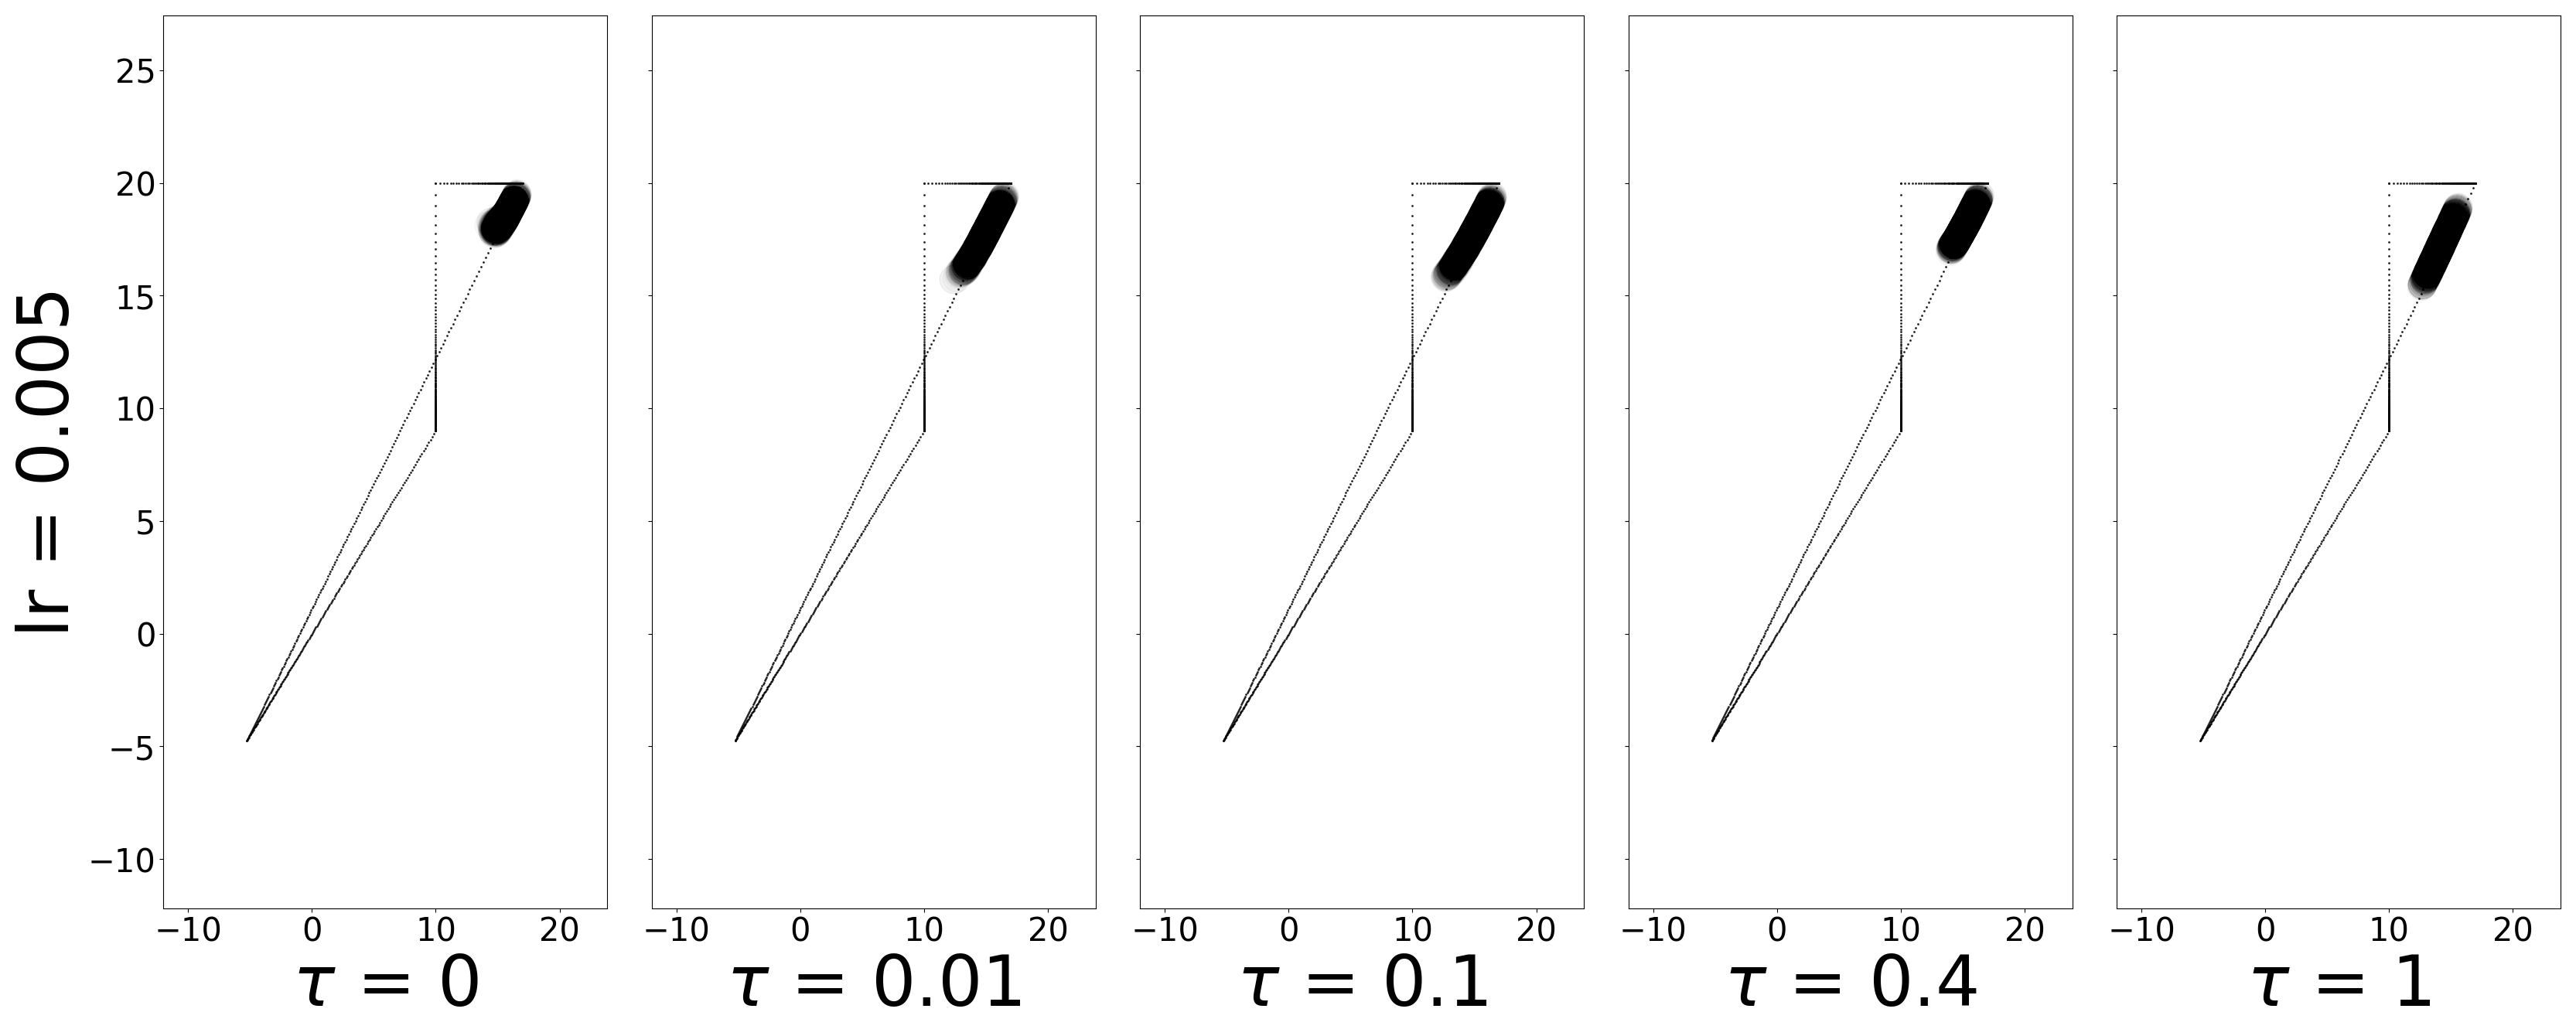
\includegraphics[width=0.8\columnwidth]{figs/switch-stay/notlearnQ/polytope_reverse_optim=adam.png}
%         \caption{Reverse KL.}
%         \label{fig:discrete-switch-stay-reverse-adam}
%   \end{subfigure}
%   \caption{Final value functions on discrete version of switch-stay after 500 gradient steps, $\gamma = 0.9$. Using Adam.}
% \end{figure}

% \begin{figure}[!htb]
%   \centering
%   \begin{subfigure}[b]{0.85\linewidth}
%     \centering
%     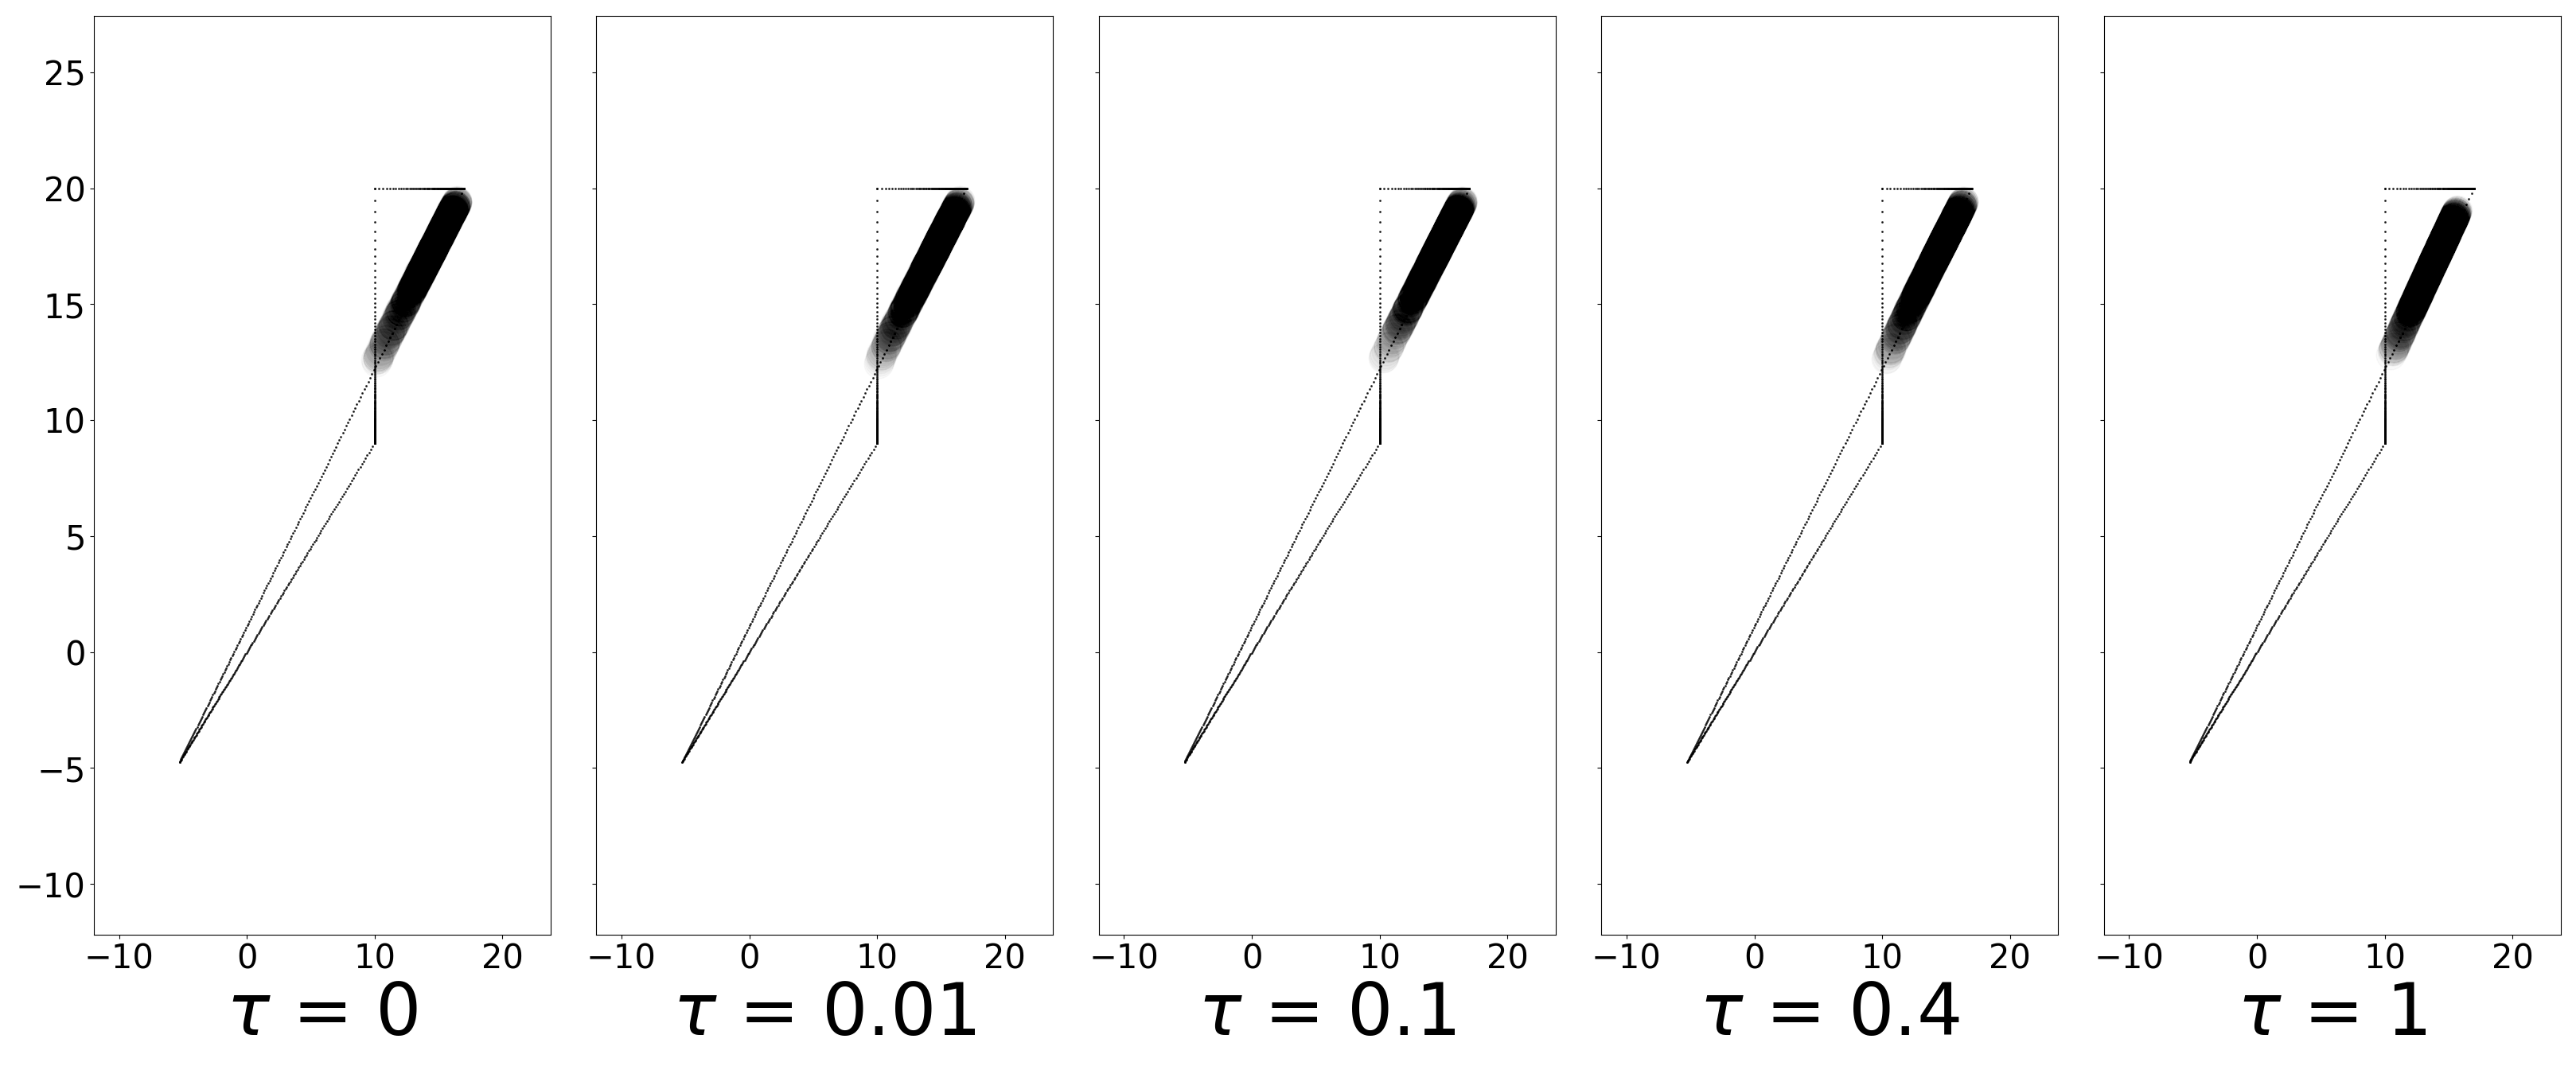
\includegraphics[width=0.8\columnwidth]{figs/switch-stay/notlearnQ/polytope_forward_optim=adam_lr=[0.005].png}
%     \caption{Forward KL, learning rate = 0.005.}
%     \label{fig:discrete-switch-stay-forward-adam0.005}
%   \end{subfigure}
  
%   \begin{subfigure}[b]{0.85\linewidth}
%         \centering
%         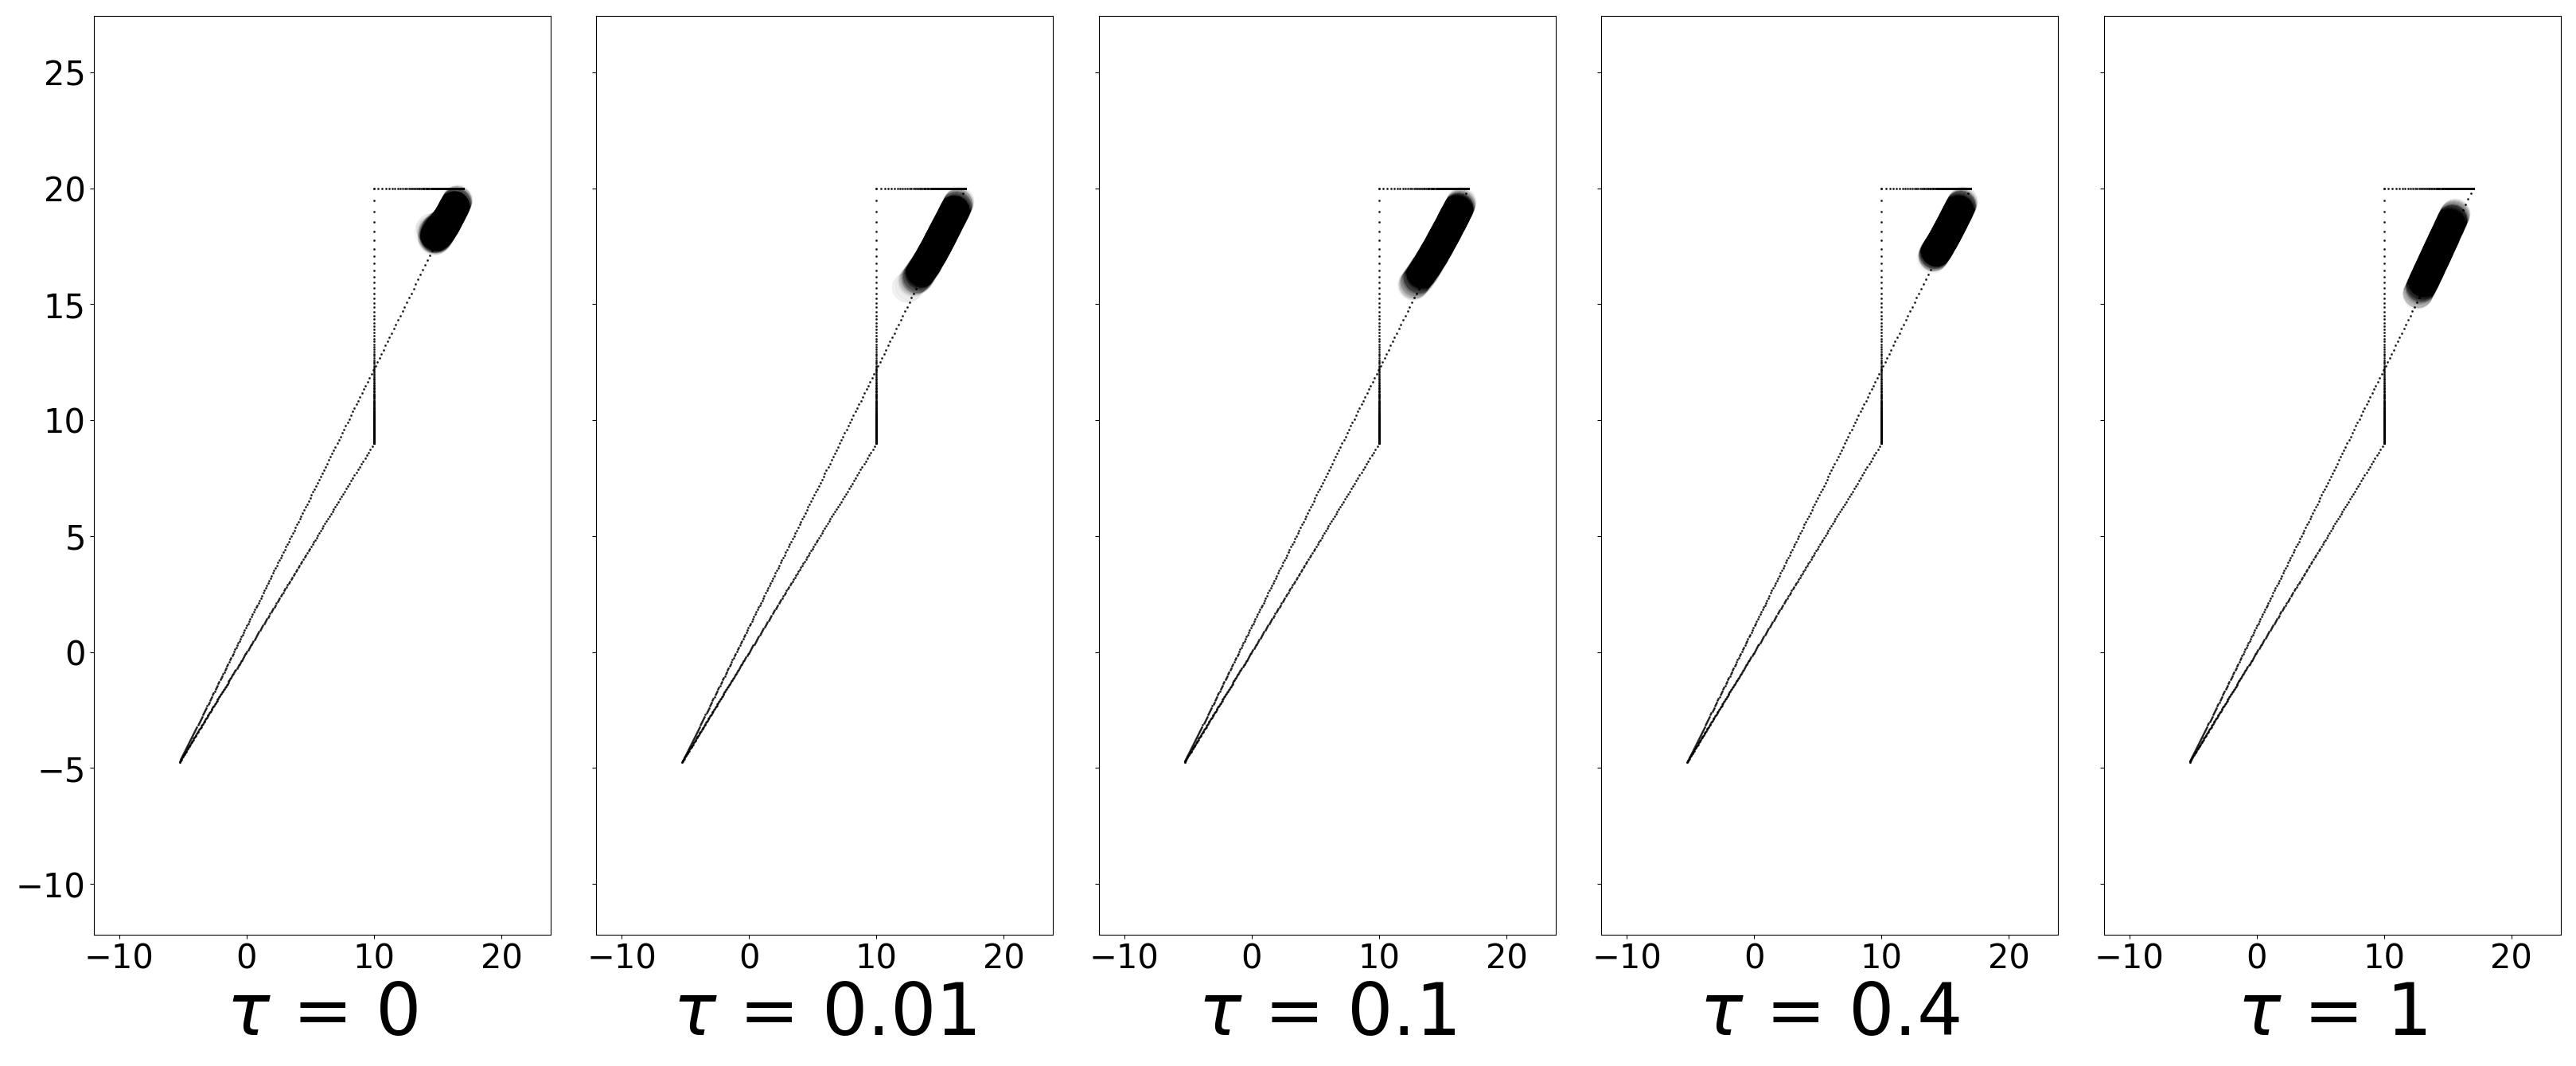
\includegraphics[width=0.8\columnwidth]{figs/switch-stay/notlearnQ/polytope_reverse_optim=adam_lr=[0.005].png}
%         \caption{Reverse KL, learning rate = 0.005.}
%         \label{fig:discrete-switch-stay-reverse-adam0.005}
%   \end{subfigure}
  
%   \begin{subfigure}[b]{0.85\linewidth}
%     \centering
%     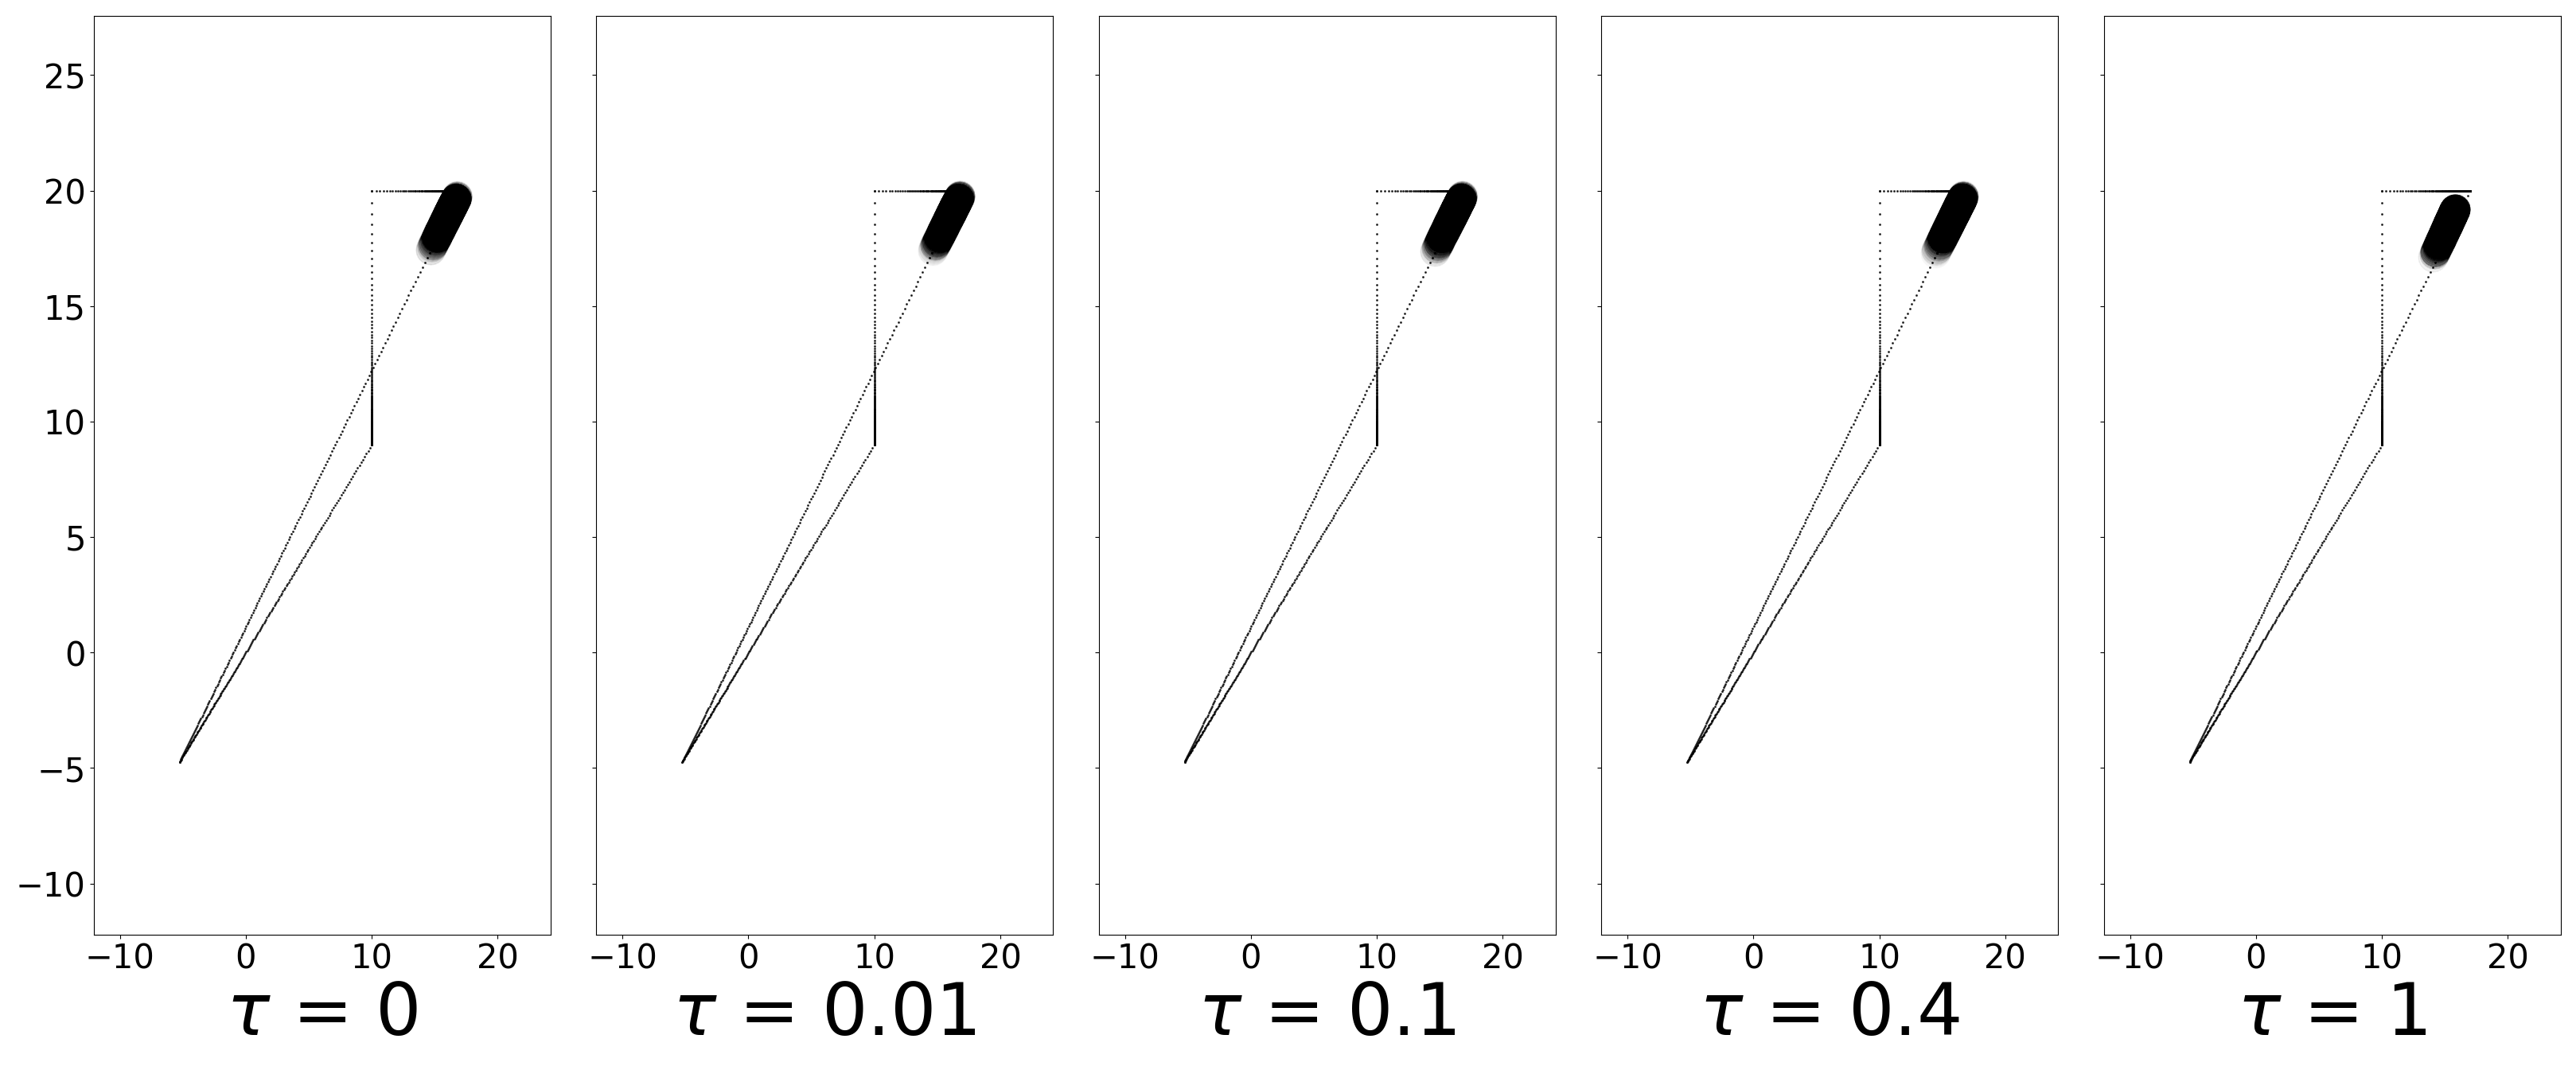
\includegraphics[width=0.8\columnwidth]{figs/switch-stay/notlearnQ/polytope_forward_optim=adam_lr=[0.01].png}
%     \caption{Forward KL, learning rate = 0.01.}
%     \label{fig:discrete-switch-stay-forward-adam0.01}
%   \end{subfigure}
  
%   \begin{subfigure}[b]{0.85\linewidth}
%         \centering
%         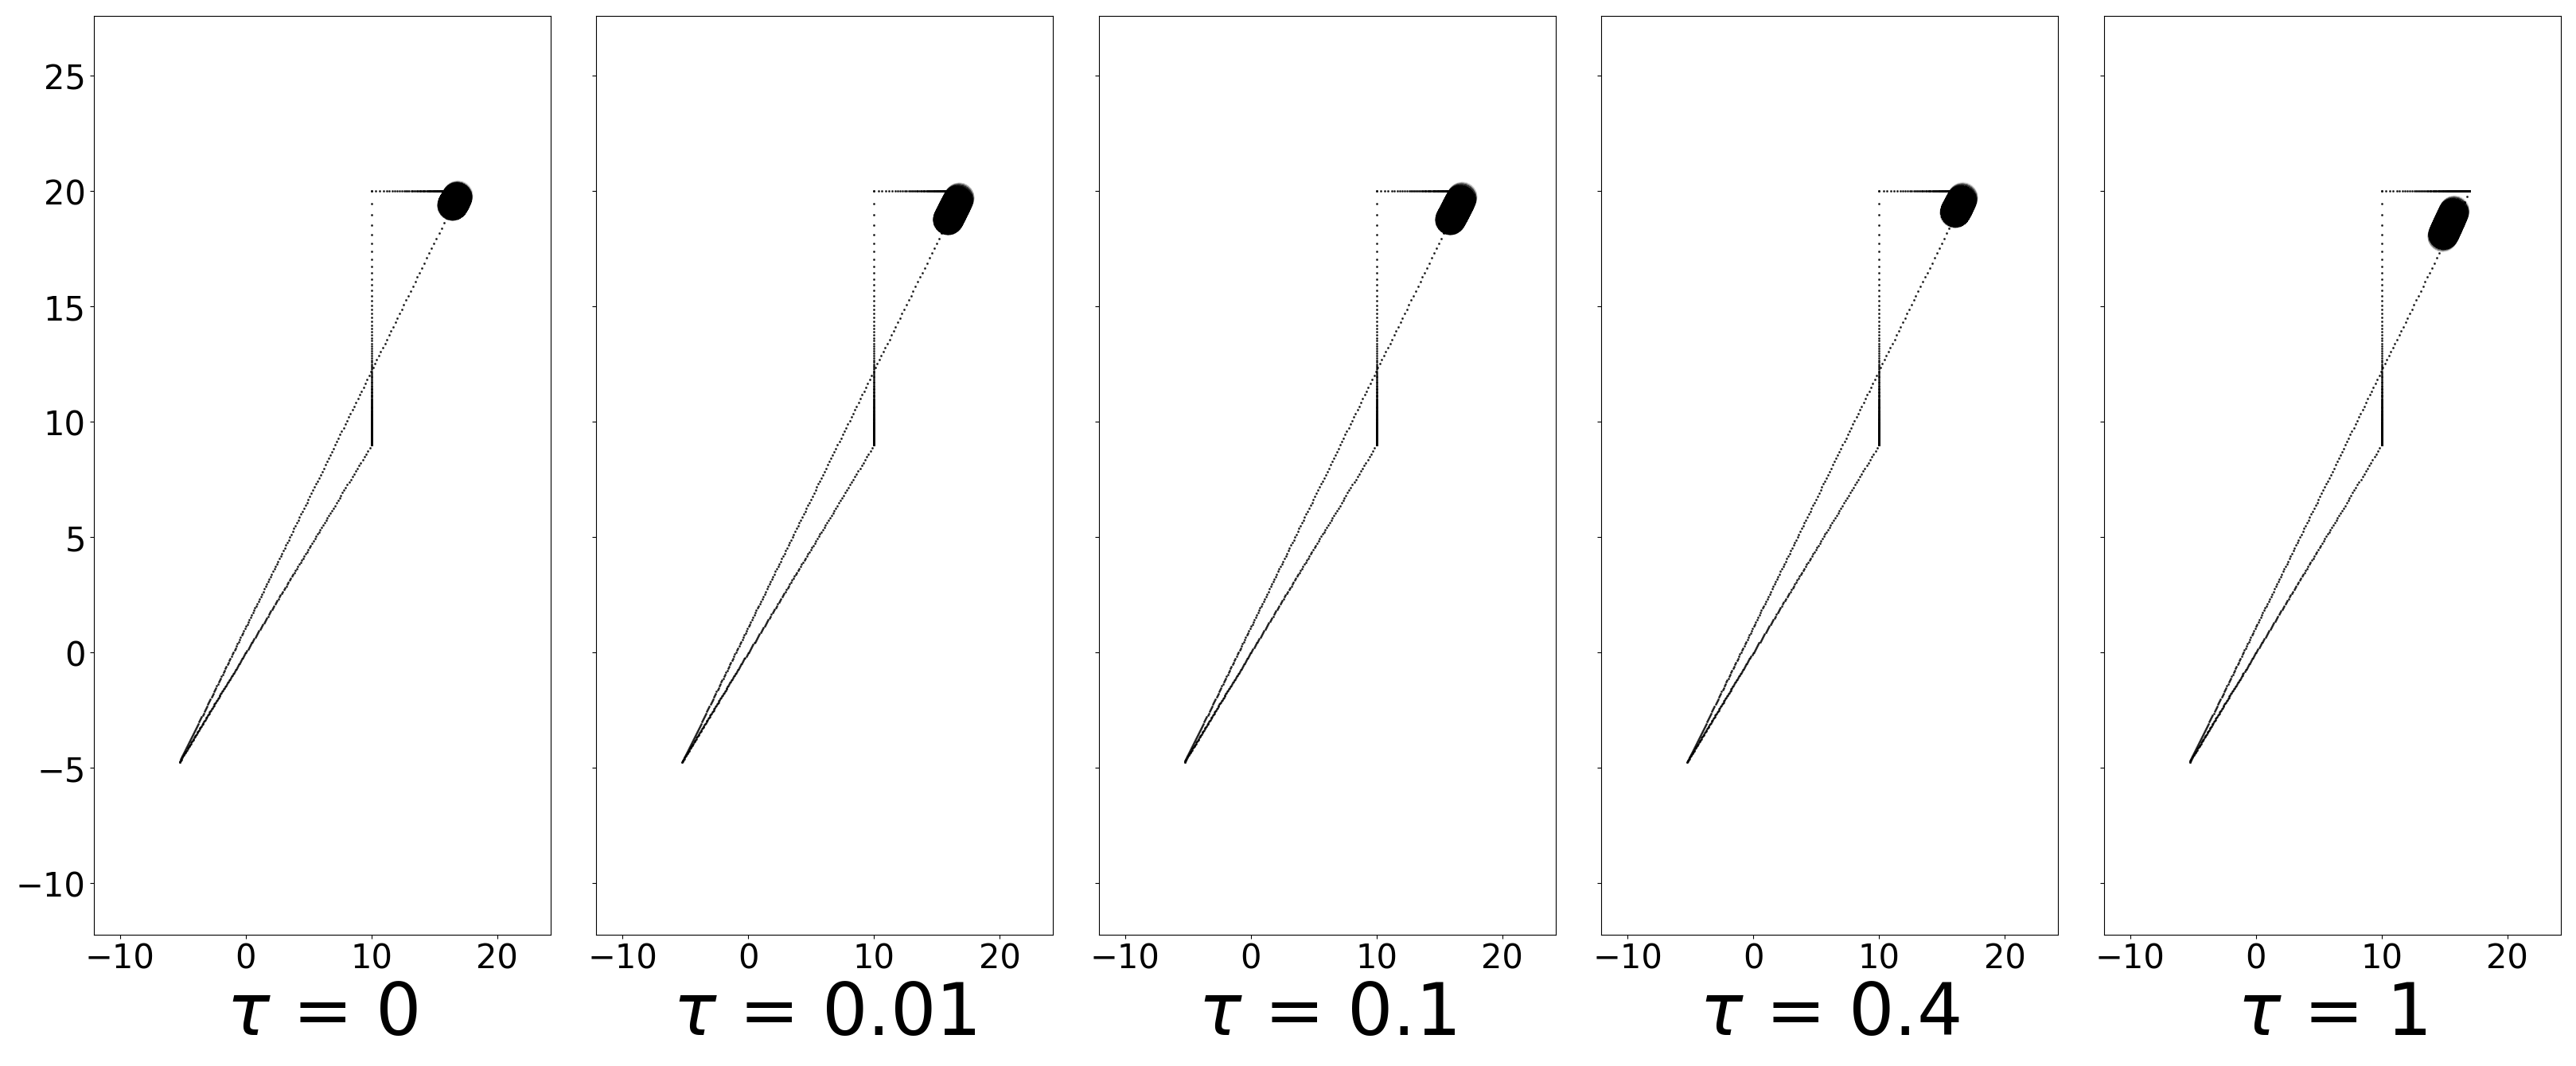
\includegraphics[width=0.8\columnwidth]{figs/switch-stay/notlearnQ/polytope_reverse_optim=adam_lr=[0.01].png}
%         \caption{Reverse KL, learning rate = 0.01.}
%         \label{fig:discrete-switch-stay-reverse-adam0.01}
%   \end{subfigure}
%   \caption{Final value functions on discrete version of switch-stay after 500 gradient steps, $\gamma = 0.9$. Using Adam for learning rates = $\{0.005, 0.01\}$.}
%   \label{fig:discrete-ss-all}
% \end{figure}


\begin{figure}[!htb]
  \centering
  \begin{subfigure}[b]{0.85\linewidth}
    \centering
    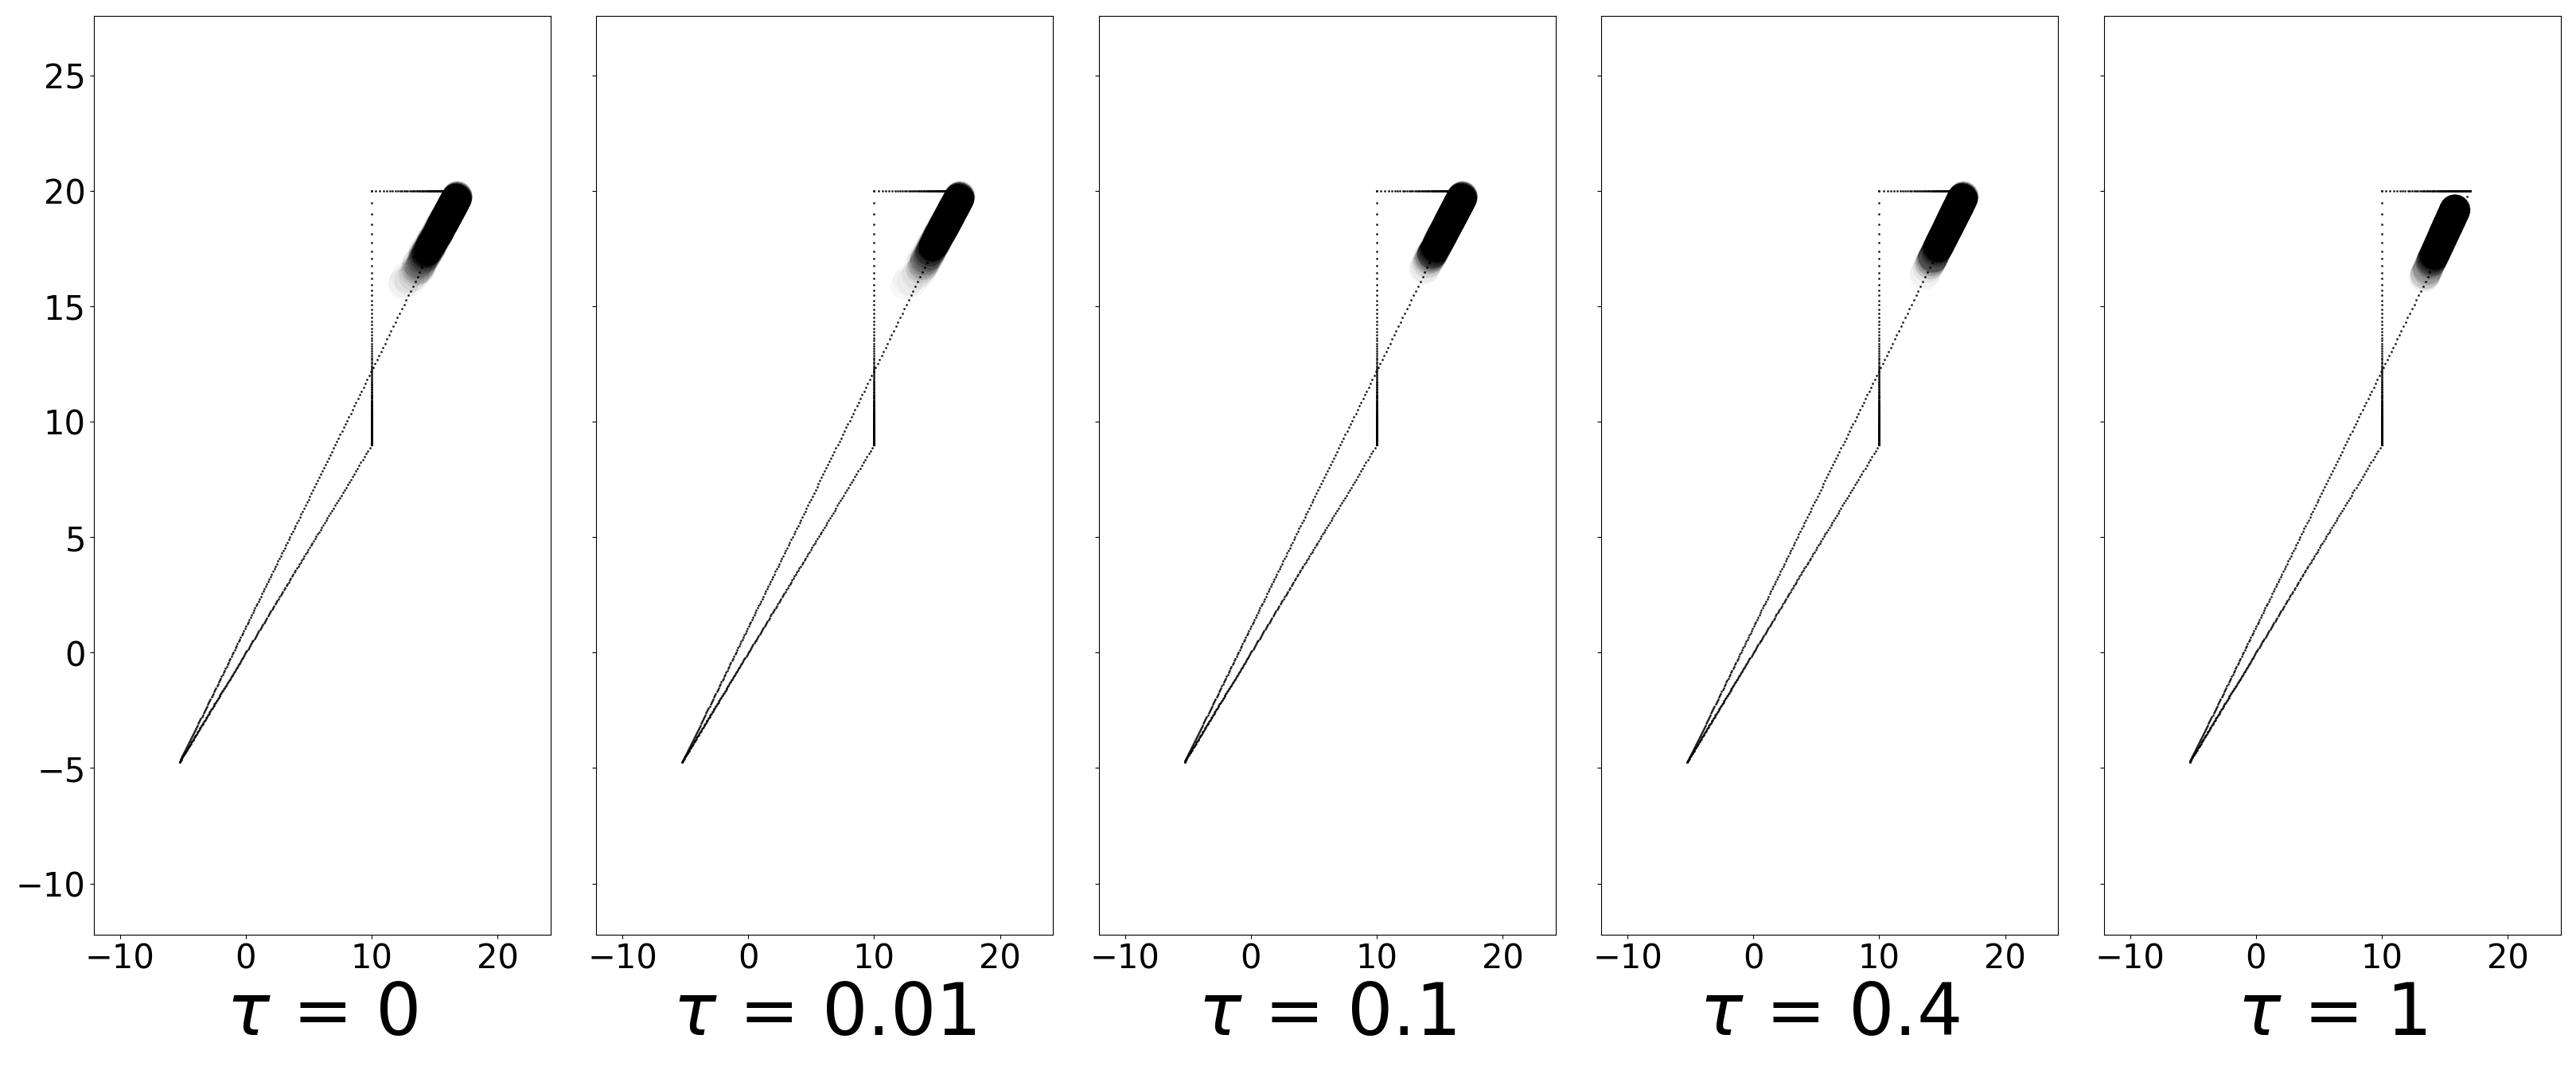
\includegraphics[width=0.8\columnwidth]{figs/switch-stay/notlearnQ/polytope_forward_optim=rmsprop_lr=[0.005].png}
    \caption{Forward KL, learning rate = 0.005.}
    \label{fig:discrete-switch-stay-forward-adam0.005}
  \end{subfigure}
  
  \begin{subfigure}[b]{0.85\linewidth}
        \centering
        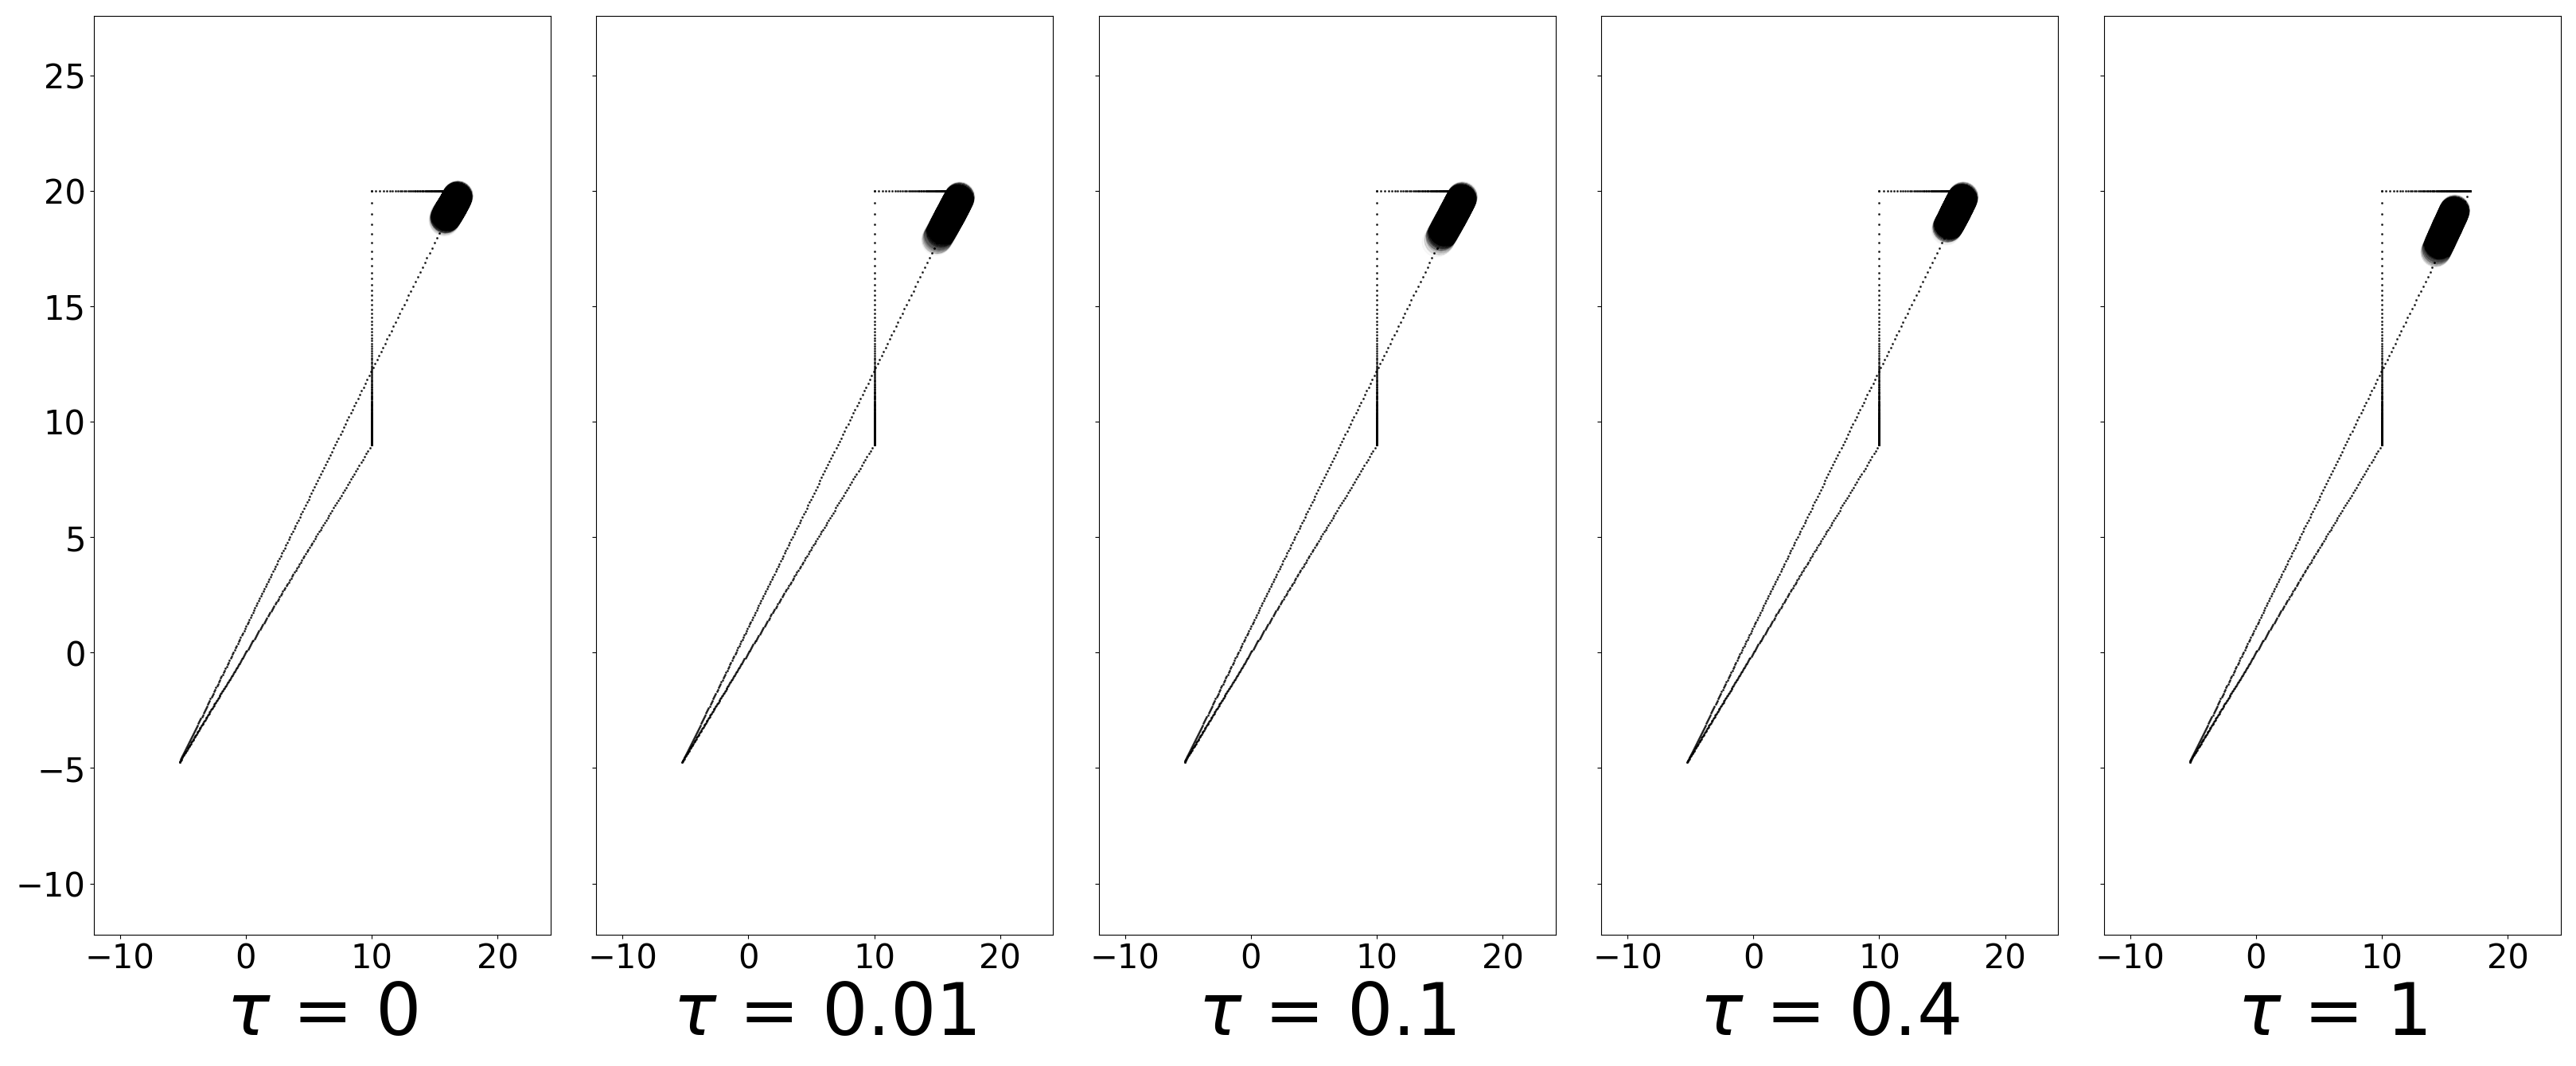
\includegraphics[width=0.8\columnwidth]{figs/switch-stay/notlearnQ/polytope_reverse_optim=rmsprop_lr=[0.005].png}
        \caption{Reverse KL, learning rate = 0.005.}
        \label{fig:discrete-switch-stay-reverse-adam0.005}
  \end{subfigure}
  
  \begin{subfigure}[b]{0.85\linewidth}
    \centering
    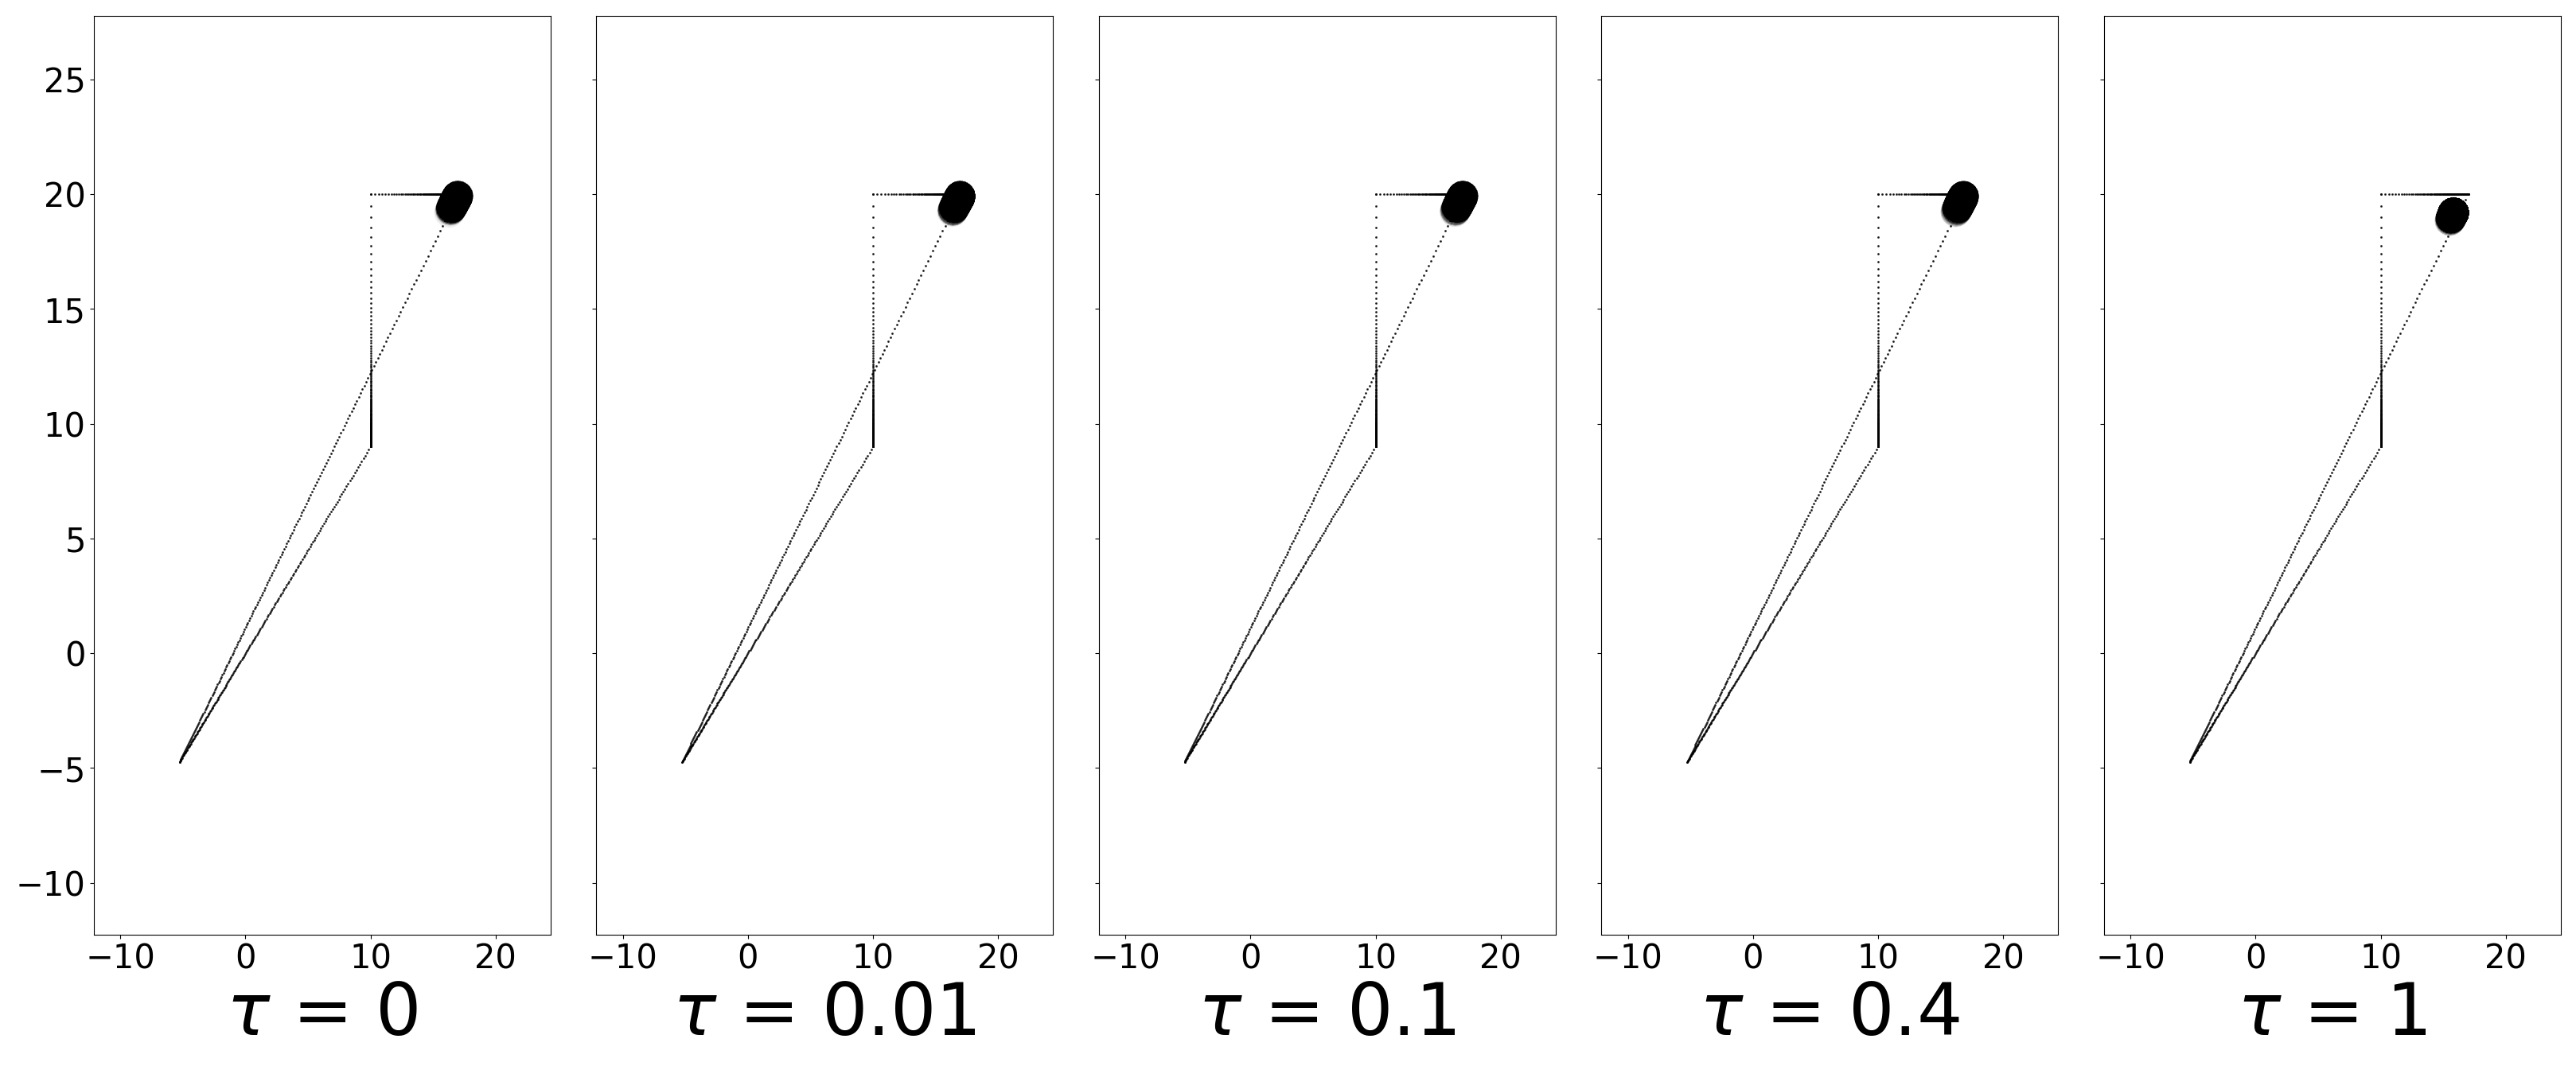
\includegraphics[width=0.8\columnwidth]{figs/switch-stay/notlearnQ/polytope_forward_optim=rmsprop_lr=[0.01].png}
    \caption{Forward KL, learning rate = 0.01.}
    \label{fig:discrete-switch-stay-forward-adam0.01}
  \end{subfigure}
  
  \begin{subfigure}[b]{0.85\linewidth}
        \centering
        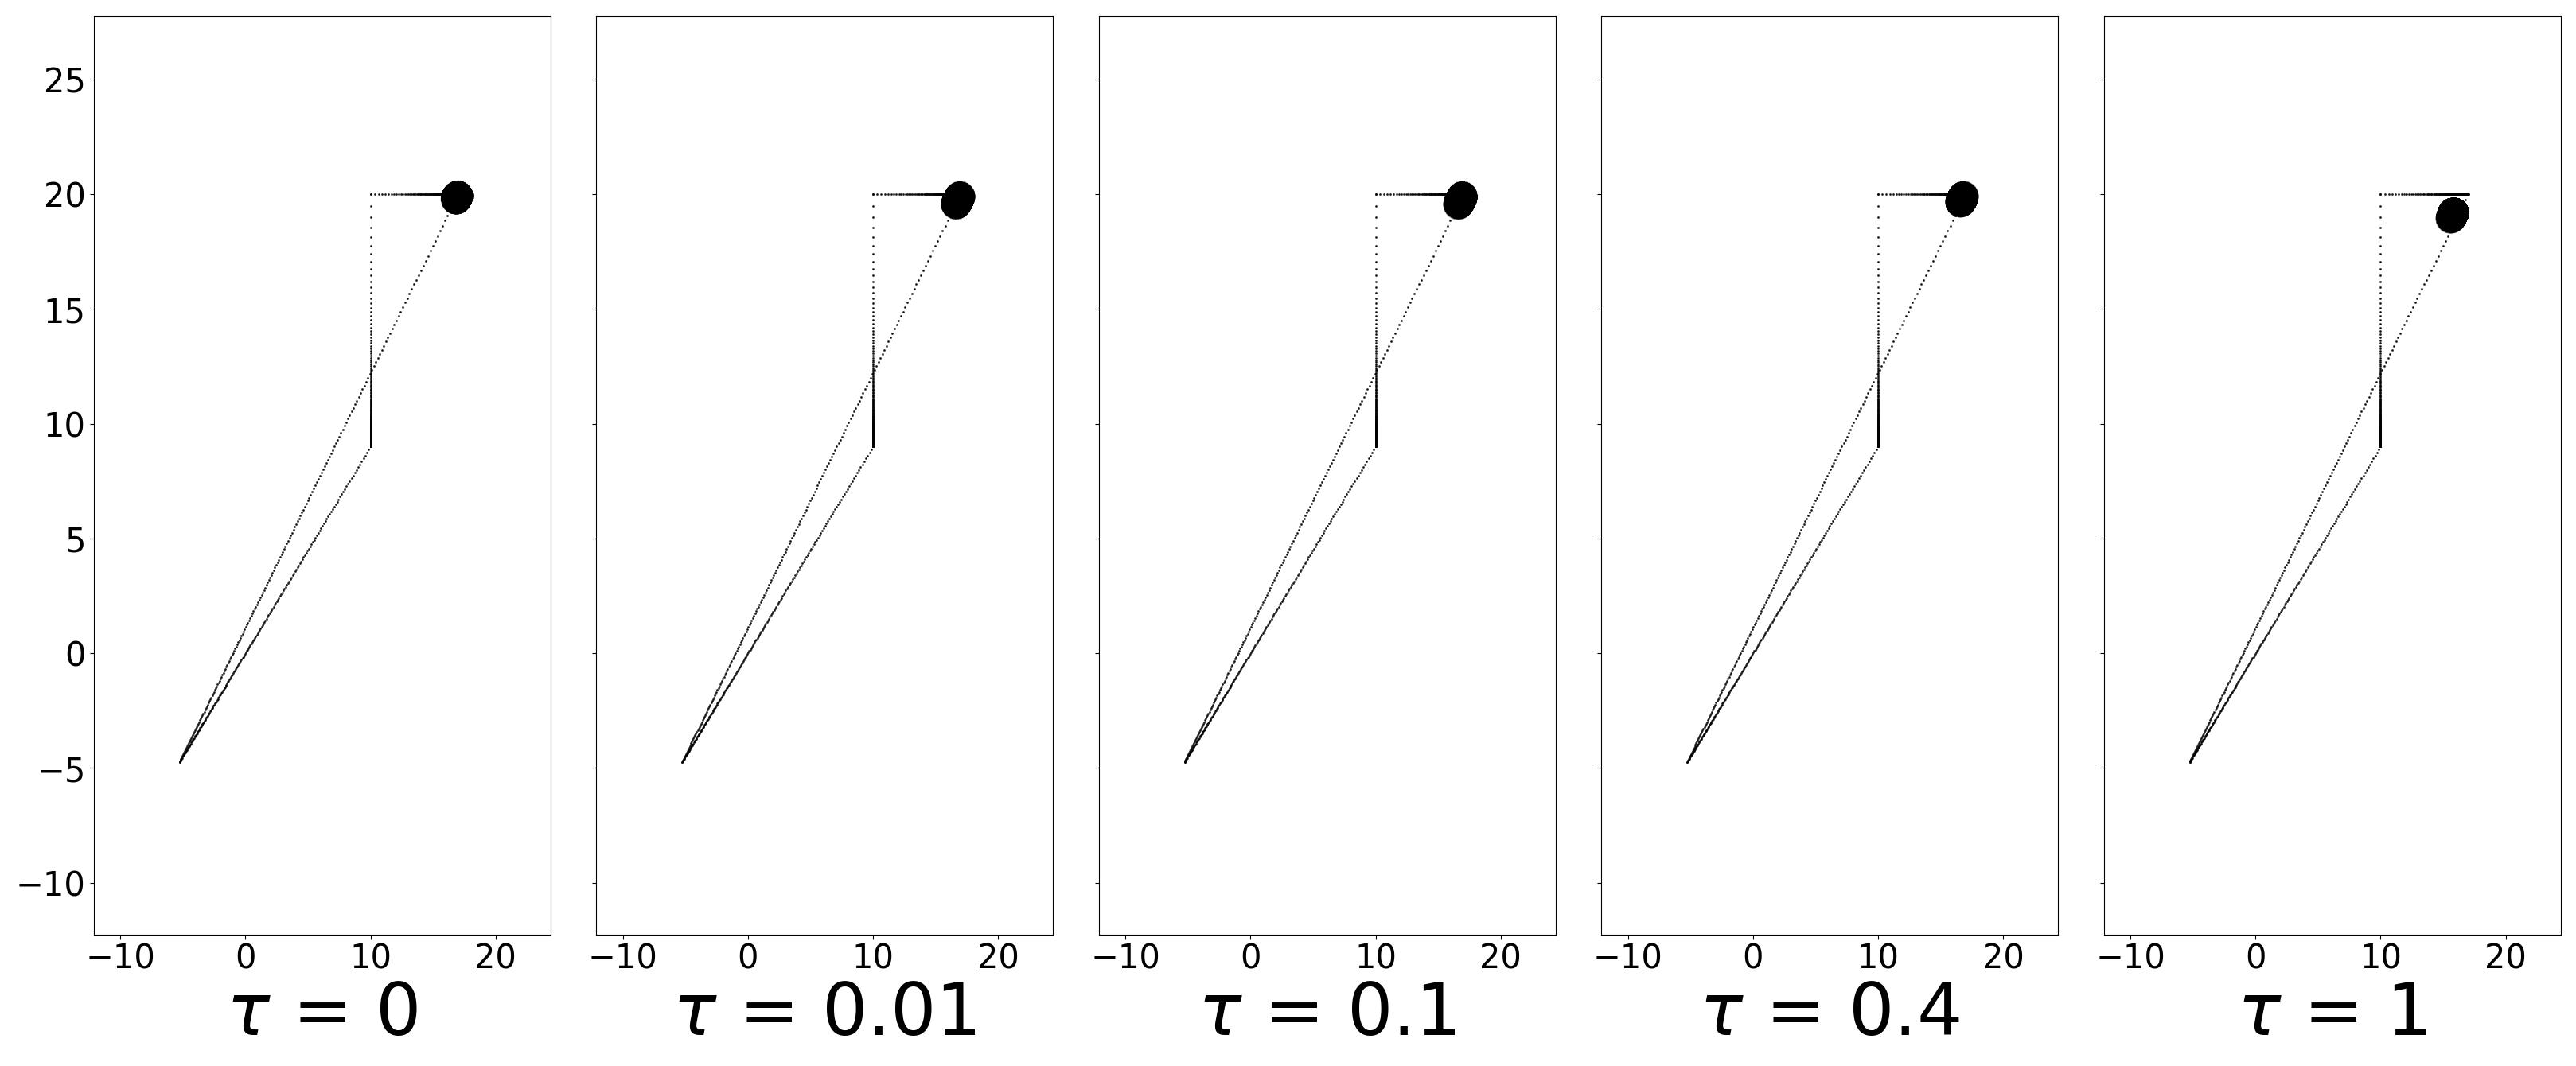
\includegraphics[width=0.8\columnwidth]{figs/switch-stay/notlearnQ/polytope_reverse_optim=rmsprop_lr=[0.01].png}
        \caption{Reverse KL, learning rate = 0.01.}
        \label{fig:discrete-switch-stay-reverse-adam0.01}
  \end{subfigure}
  \caption{Final value functions on discrete version of switch-stay after 500 gradient steps, $\gamma = 0.9$. Using RMSprop for learning rates $\in \{0.005, 0.01\}$.}
  \label{fig:discrete-ss-all}
\end{figure}


\subsection{The Impact of Stochasticity}\label{sec:stochastic-microworld}
Although with discrete actions it is practical to sum across all actions when calculating the KL losses, difficulty emerges with high-dimensional continuous action spaces. Quadrature methods scale exponentially with the dimension of the action-space, leaving methods like Clenshaw-Curtis impractical; Monte-Carlo integration seems the only feasible answer in this setting. 

We repeated the continuous-action microworld experiments to understand any differences induced by using Monte-Carlo integration (i.e., sampling actions from the current policy) instead of Clenshaw-Curtis quadrature to calculate the losses. 

Since Hard FKL only depends upon the maximum action, we do not modify the algorithm in this regime. Hard and soft RKL are modified to use sampled actions from the current policy $\pi$. To derive a sampling-based version of soft FKL, we use weighted importance sampling to approximate the integral $-\int_\actionspace \boltzmannQ(s, a) \log \pi(a \mid s)\, da$, noting that the omitted term $\entropy(\boltzmannQ(\cdot \mid s))$ does not depend on $\pi$. In particular, for samples $\{a_i\}_{i = 1}^n \sim \pi(\cdot \mid s)$ we estimate 
\begin{align*}
    -\int_\actionspace \boltzmannQ(s, a) \log \pi(a \mid s)\, da &\approx \sum_{i = 1}^n \rho_i \log \pi(a_i \mid s) ,\\
    \rho_i &:= \frac{\tilde{\rho}_i}{\sum_{j = 1}^n \tilde{\rho}_j}\\
    \tilde{\rho}_i &:= \frac{\exp(Q(s, a_i) \tau^{-1})}{\pi(a_i \mid s)}. 
\end{align*}
Note that we do not have to estimate $\entropy(\boltzmannQ(s, \cdot))$, the other term in the FKL, as it does not depend on $\pi$. Weighted importance sampling lets us avoid calculating the partition function in $\boltzmannQ$, and may be a fruitful avenue to explore in making FKL practical for high-dimensional action spaces. 

% \begin{figure}[!htb]
%   \centering
%   \begin{subfigure}[b]{0.85\linewidth}
%     \centering
%     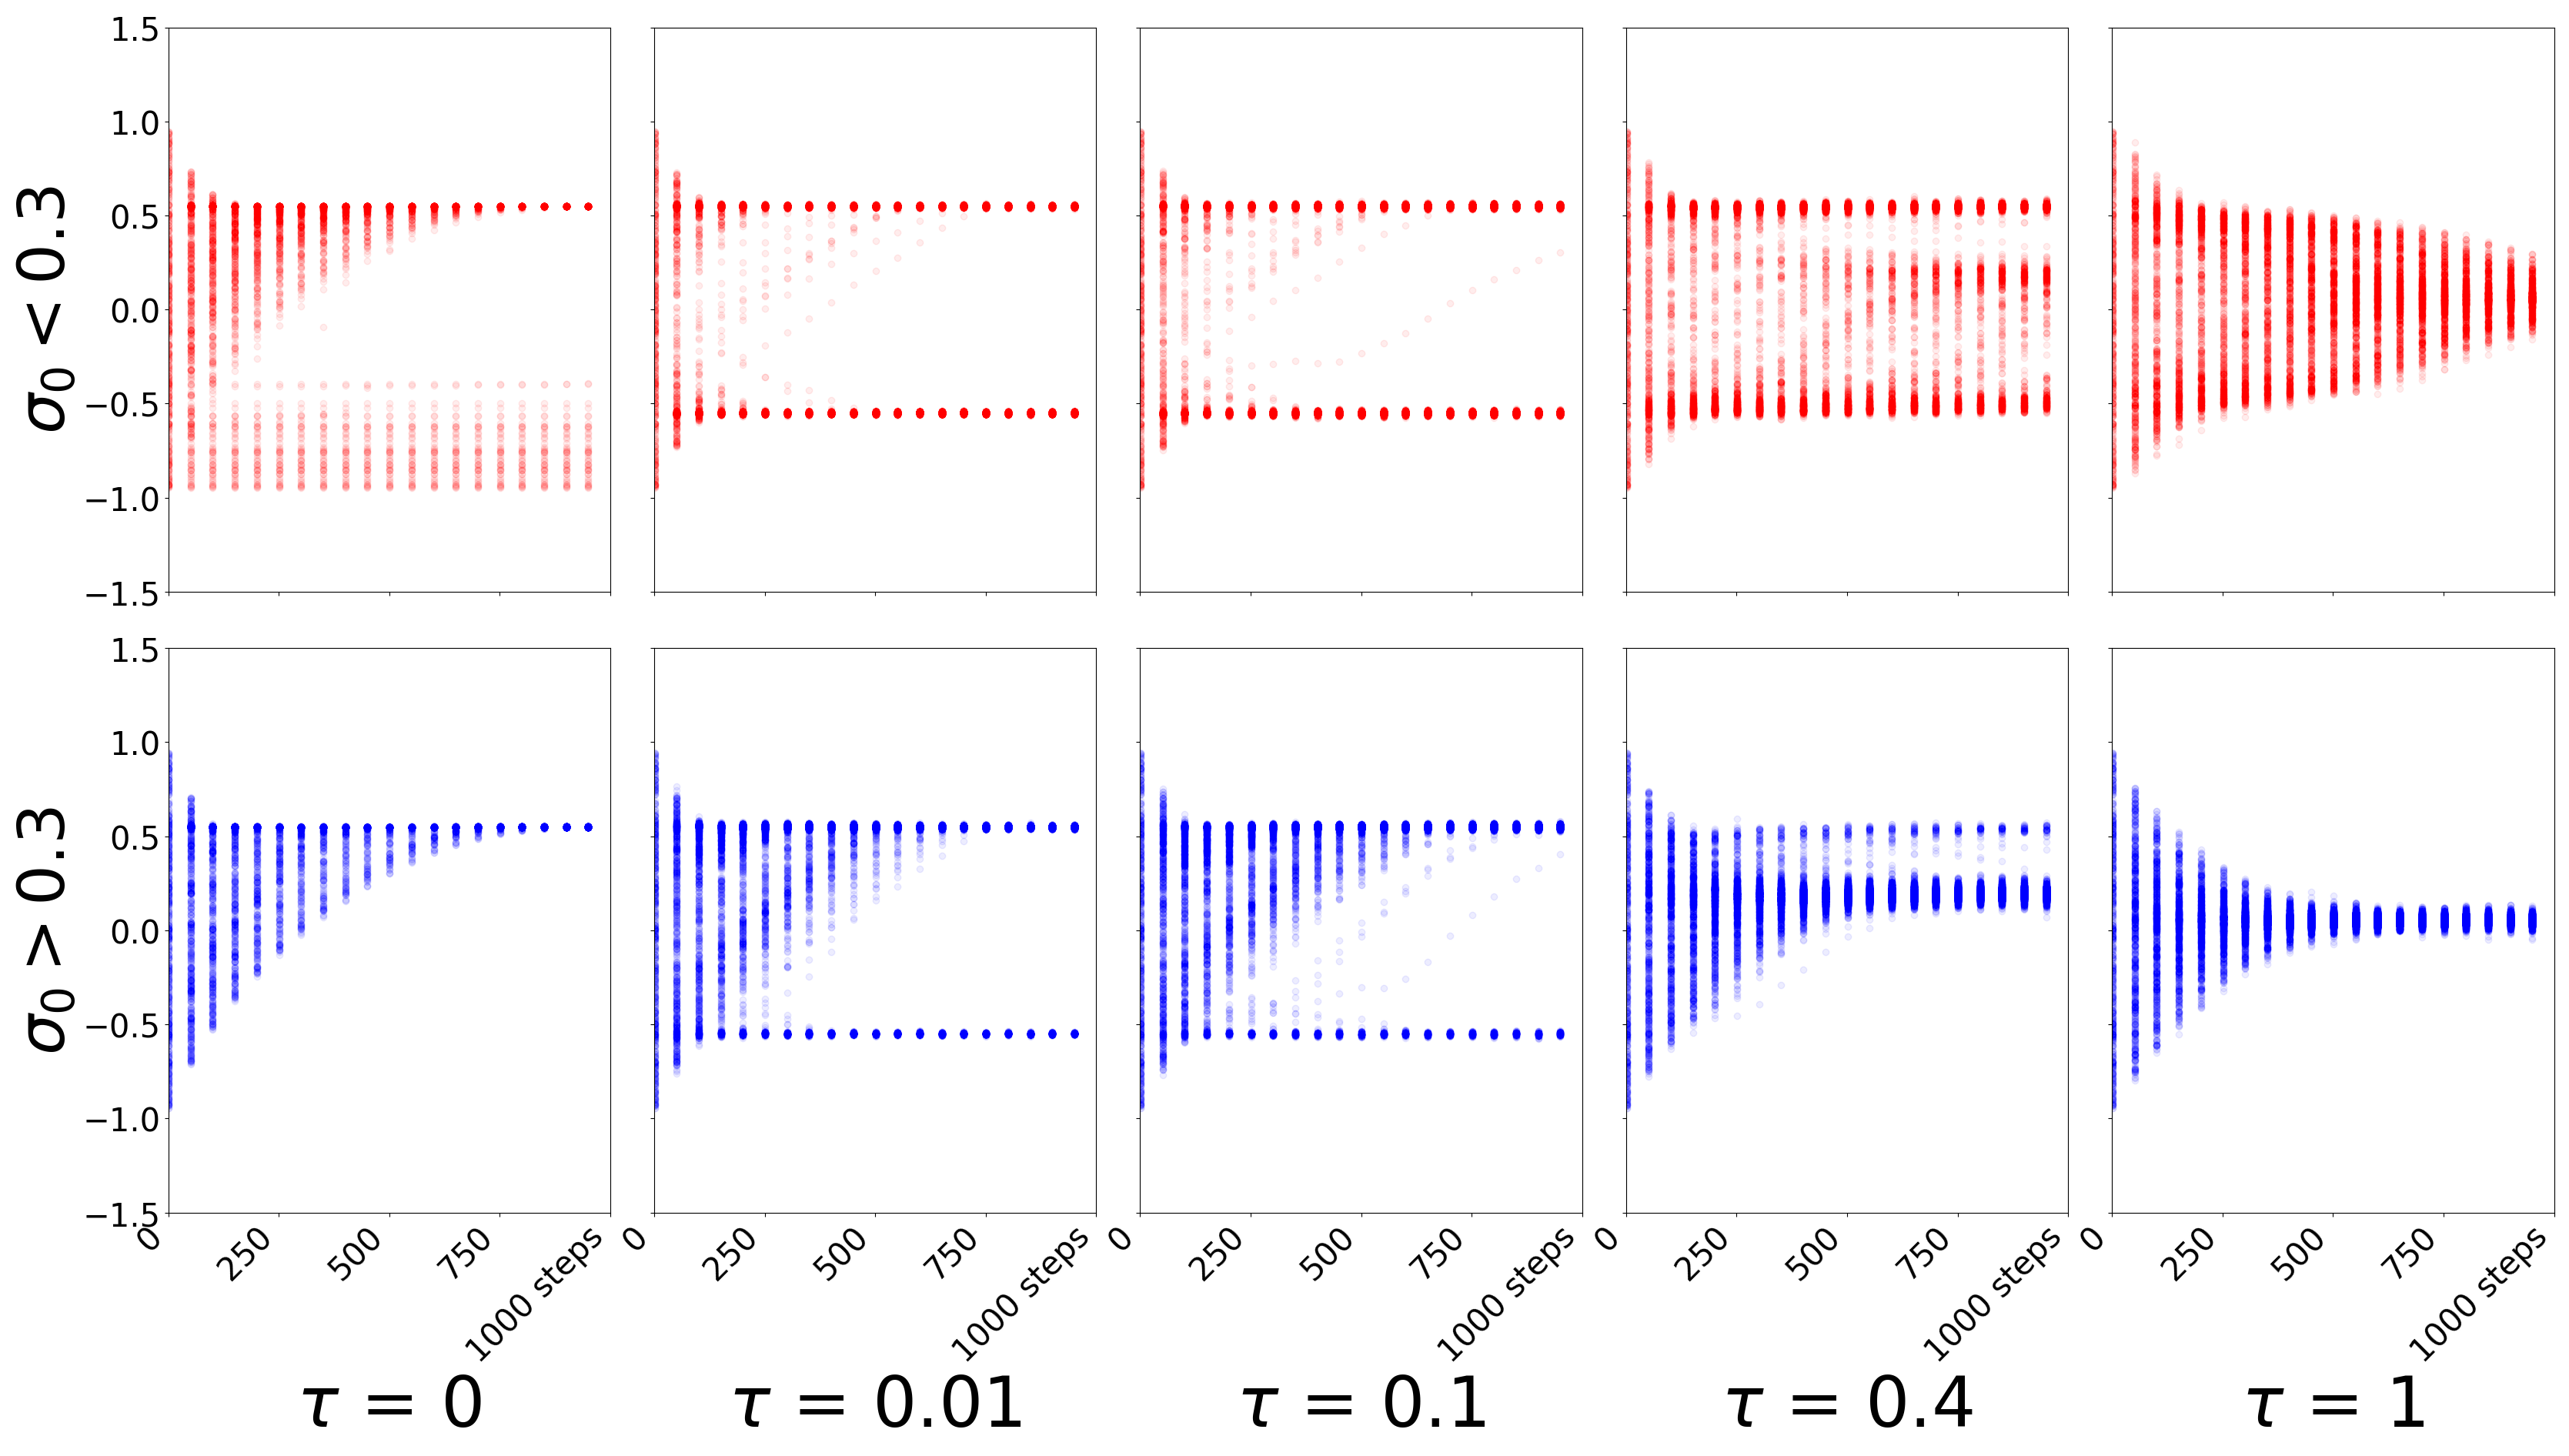
\includegraphics[width=0.8\columnwidth]{figs/bandit/monte-carlo/10/mean_forward_optim=adam_modes=1_lr=0.005.png}
%     \caption{Forward KL.}
%     \label{fig:10-sample-cont-bandit-forward}
%   \end{subfigure}
  
%   \begin{subfigure}[b]{0.85\linewidth}
%         \centering
%         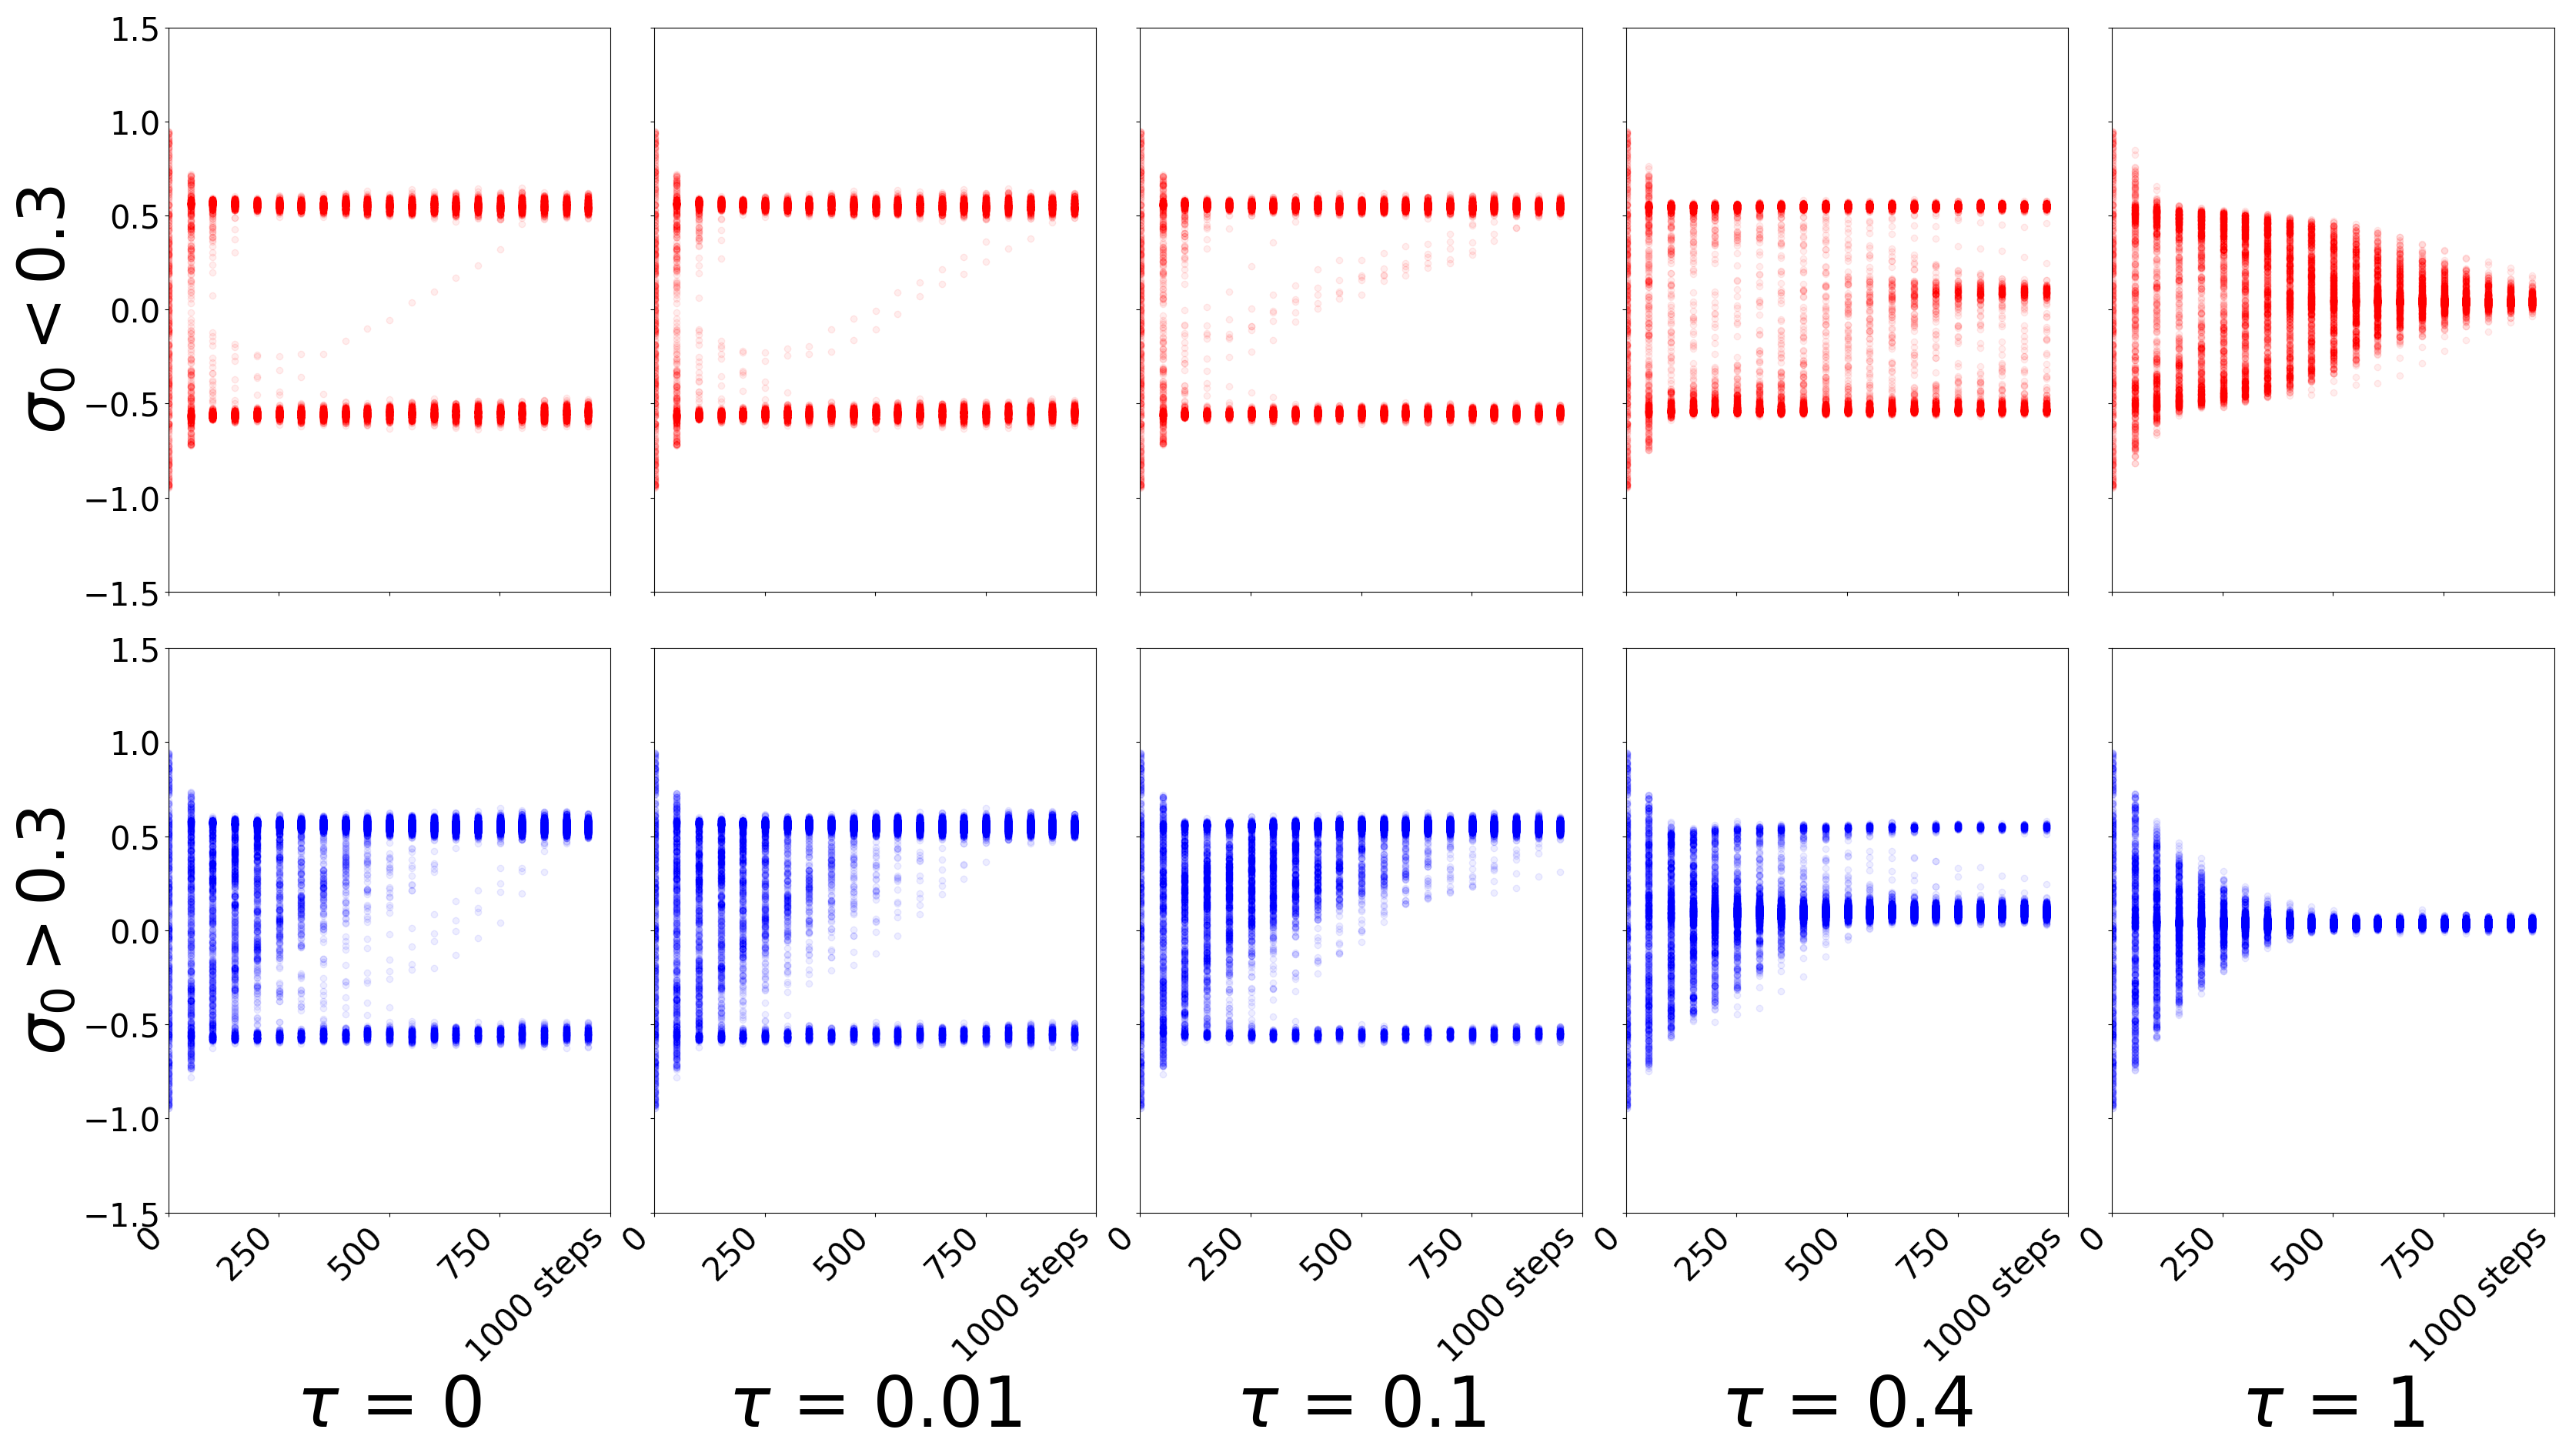
\includegraphics[width=0.8\columnwidth]{figs/bandit/monte-carlo/10/mean_reverse_optim=adam_modes=1_lr=0.005.png}
%         \caption{Reverse KL.}
%         \label{fig:10-sample-cont-bandit-reverse}
%   \end{subfigure}
%   \caption{Continuous bandit with 10 sample points, learning rate = 0.005, with Adam.}
% \end{figure}


\begin{figure}[!htb]
  \centering
  \begin{subfigure}[b]{0.85\linewidth}
    \centering
    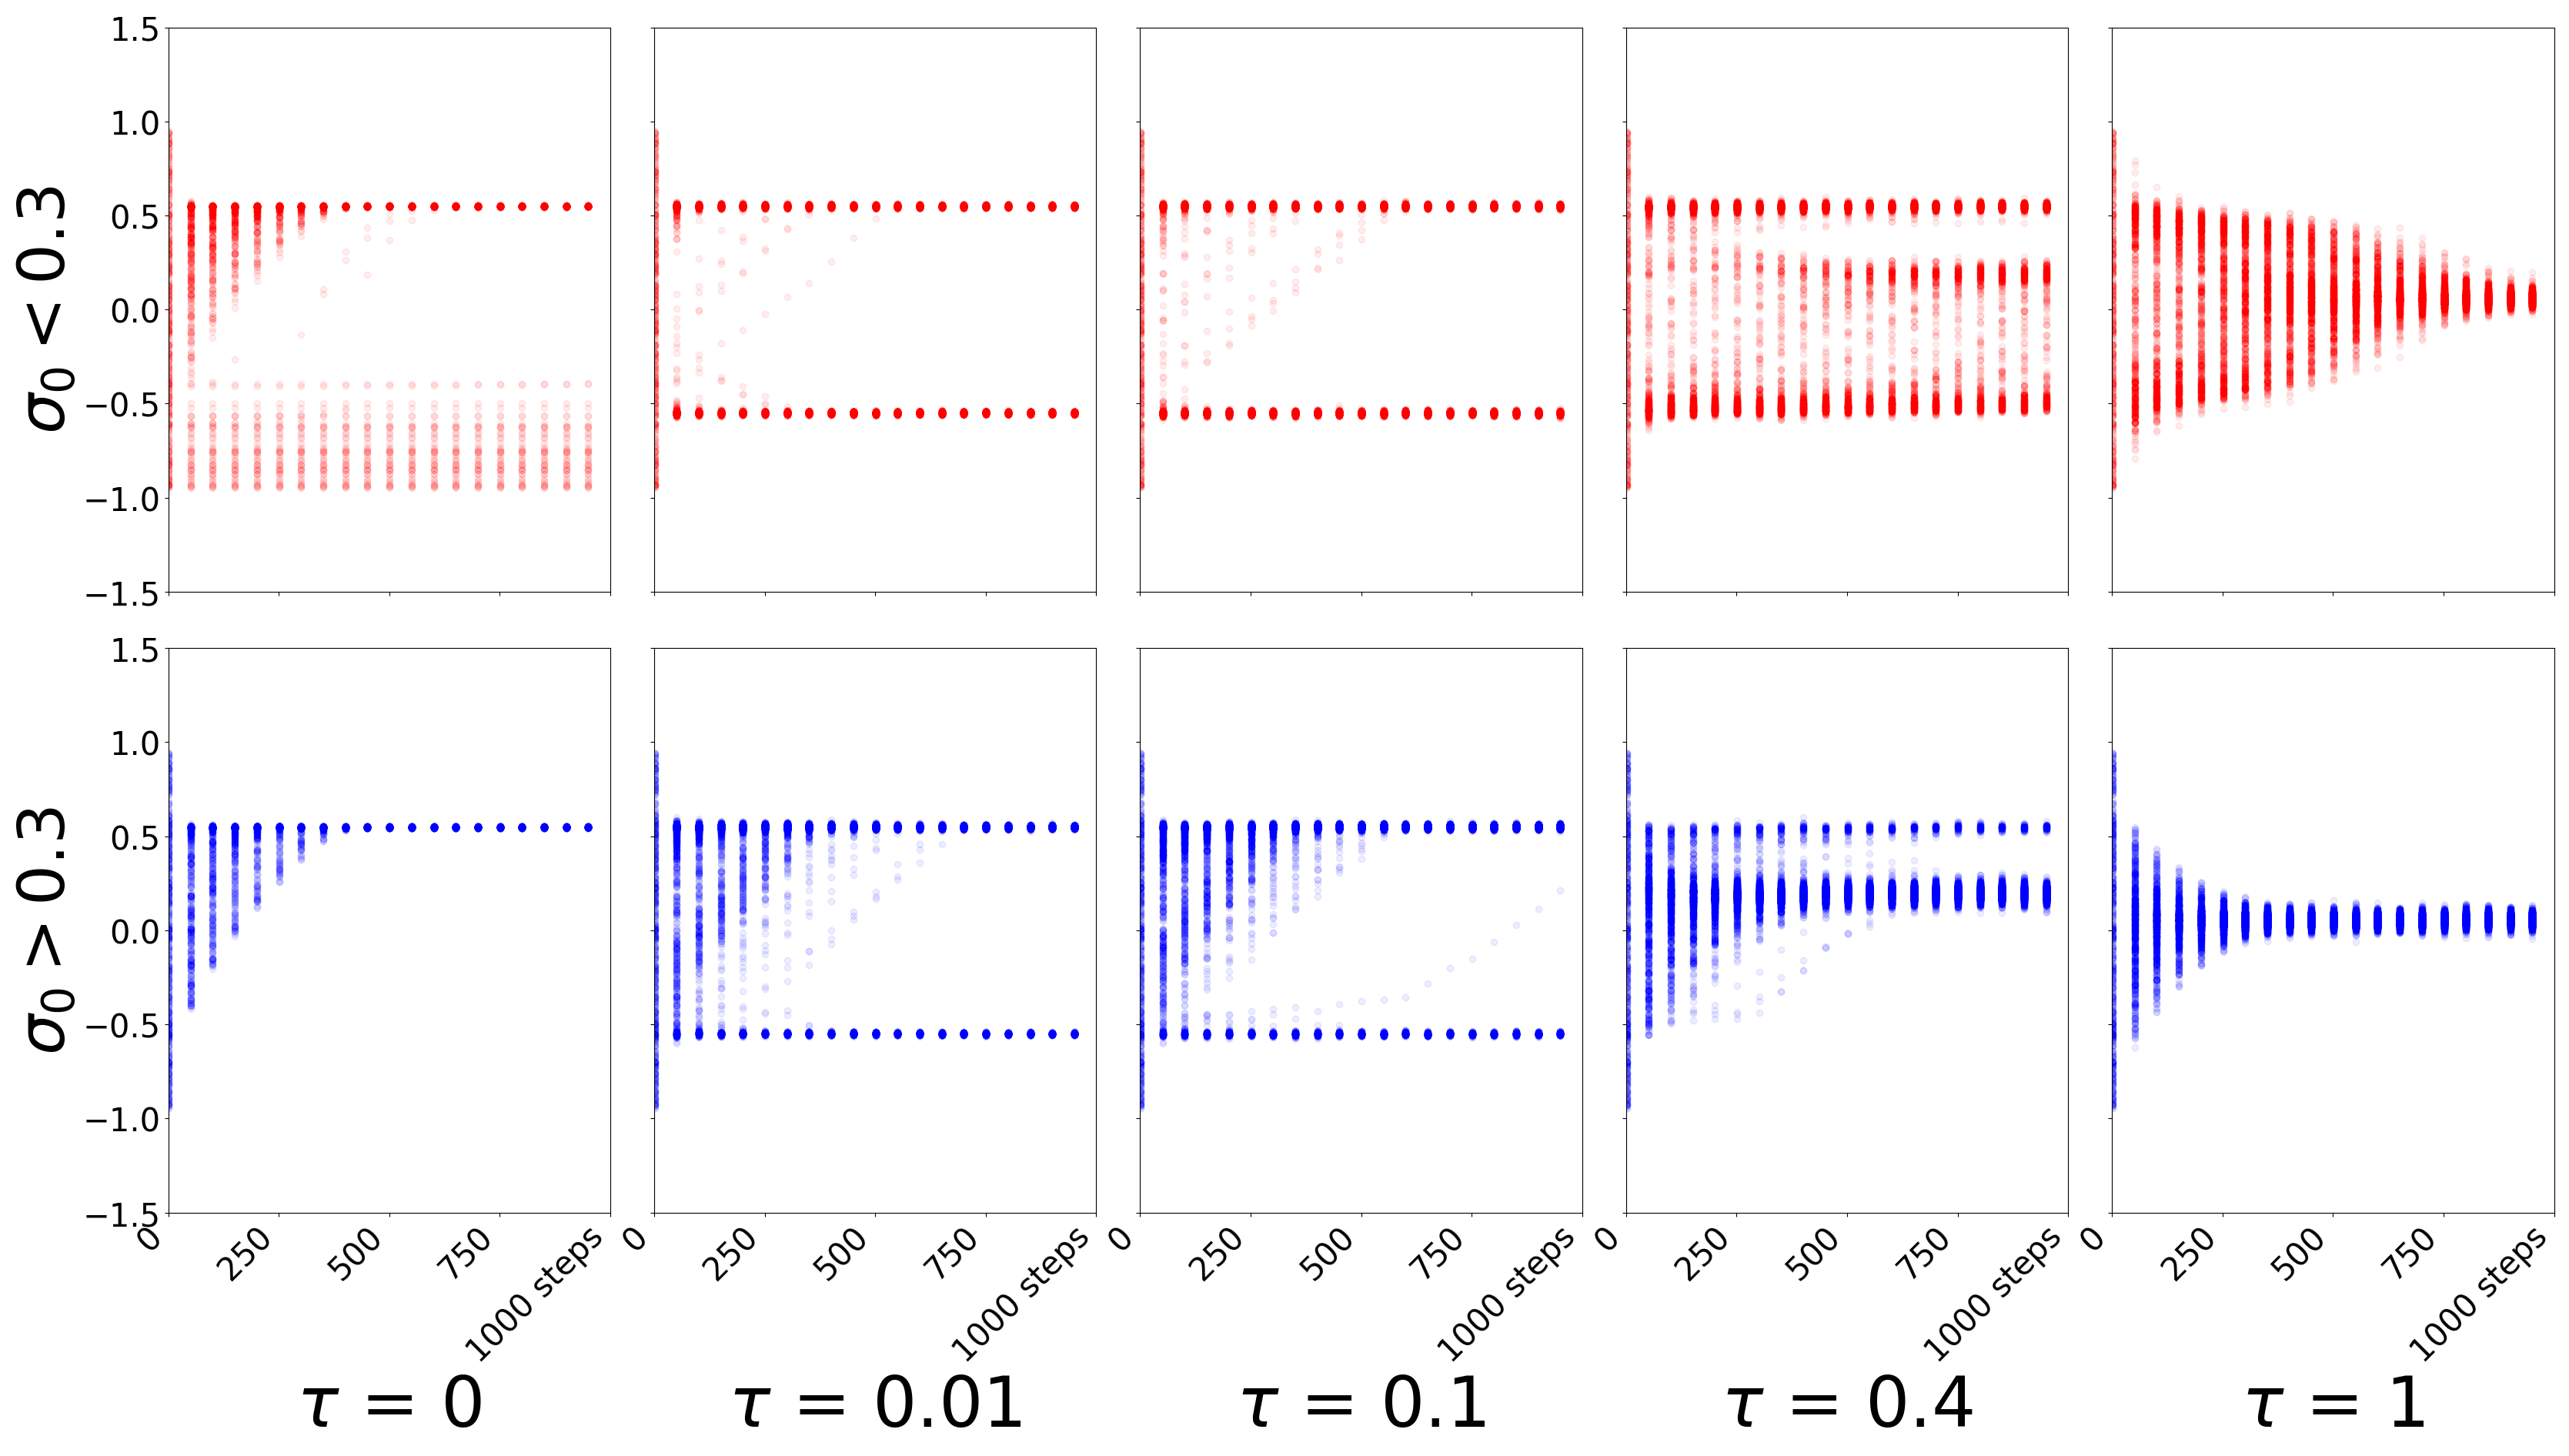
\includegraphics[width=0.8\columnwidth]{figs/bandit/monte-carlo/10/mean_forward_optim=rmsprop_modes=1_lr=0.005.png}
    \caption{Forward KL.}
    \label{fig:10-sample-cont-bandit-forward}
  \end{subfigure}
  
  \begin{subfigure}[b]{0.85\linewidth}
        \centering
        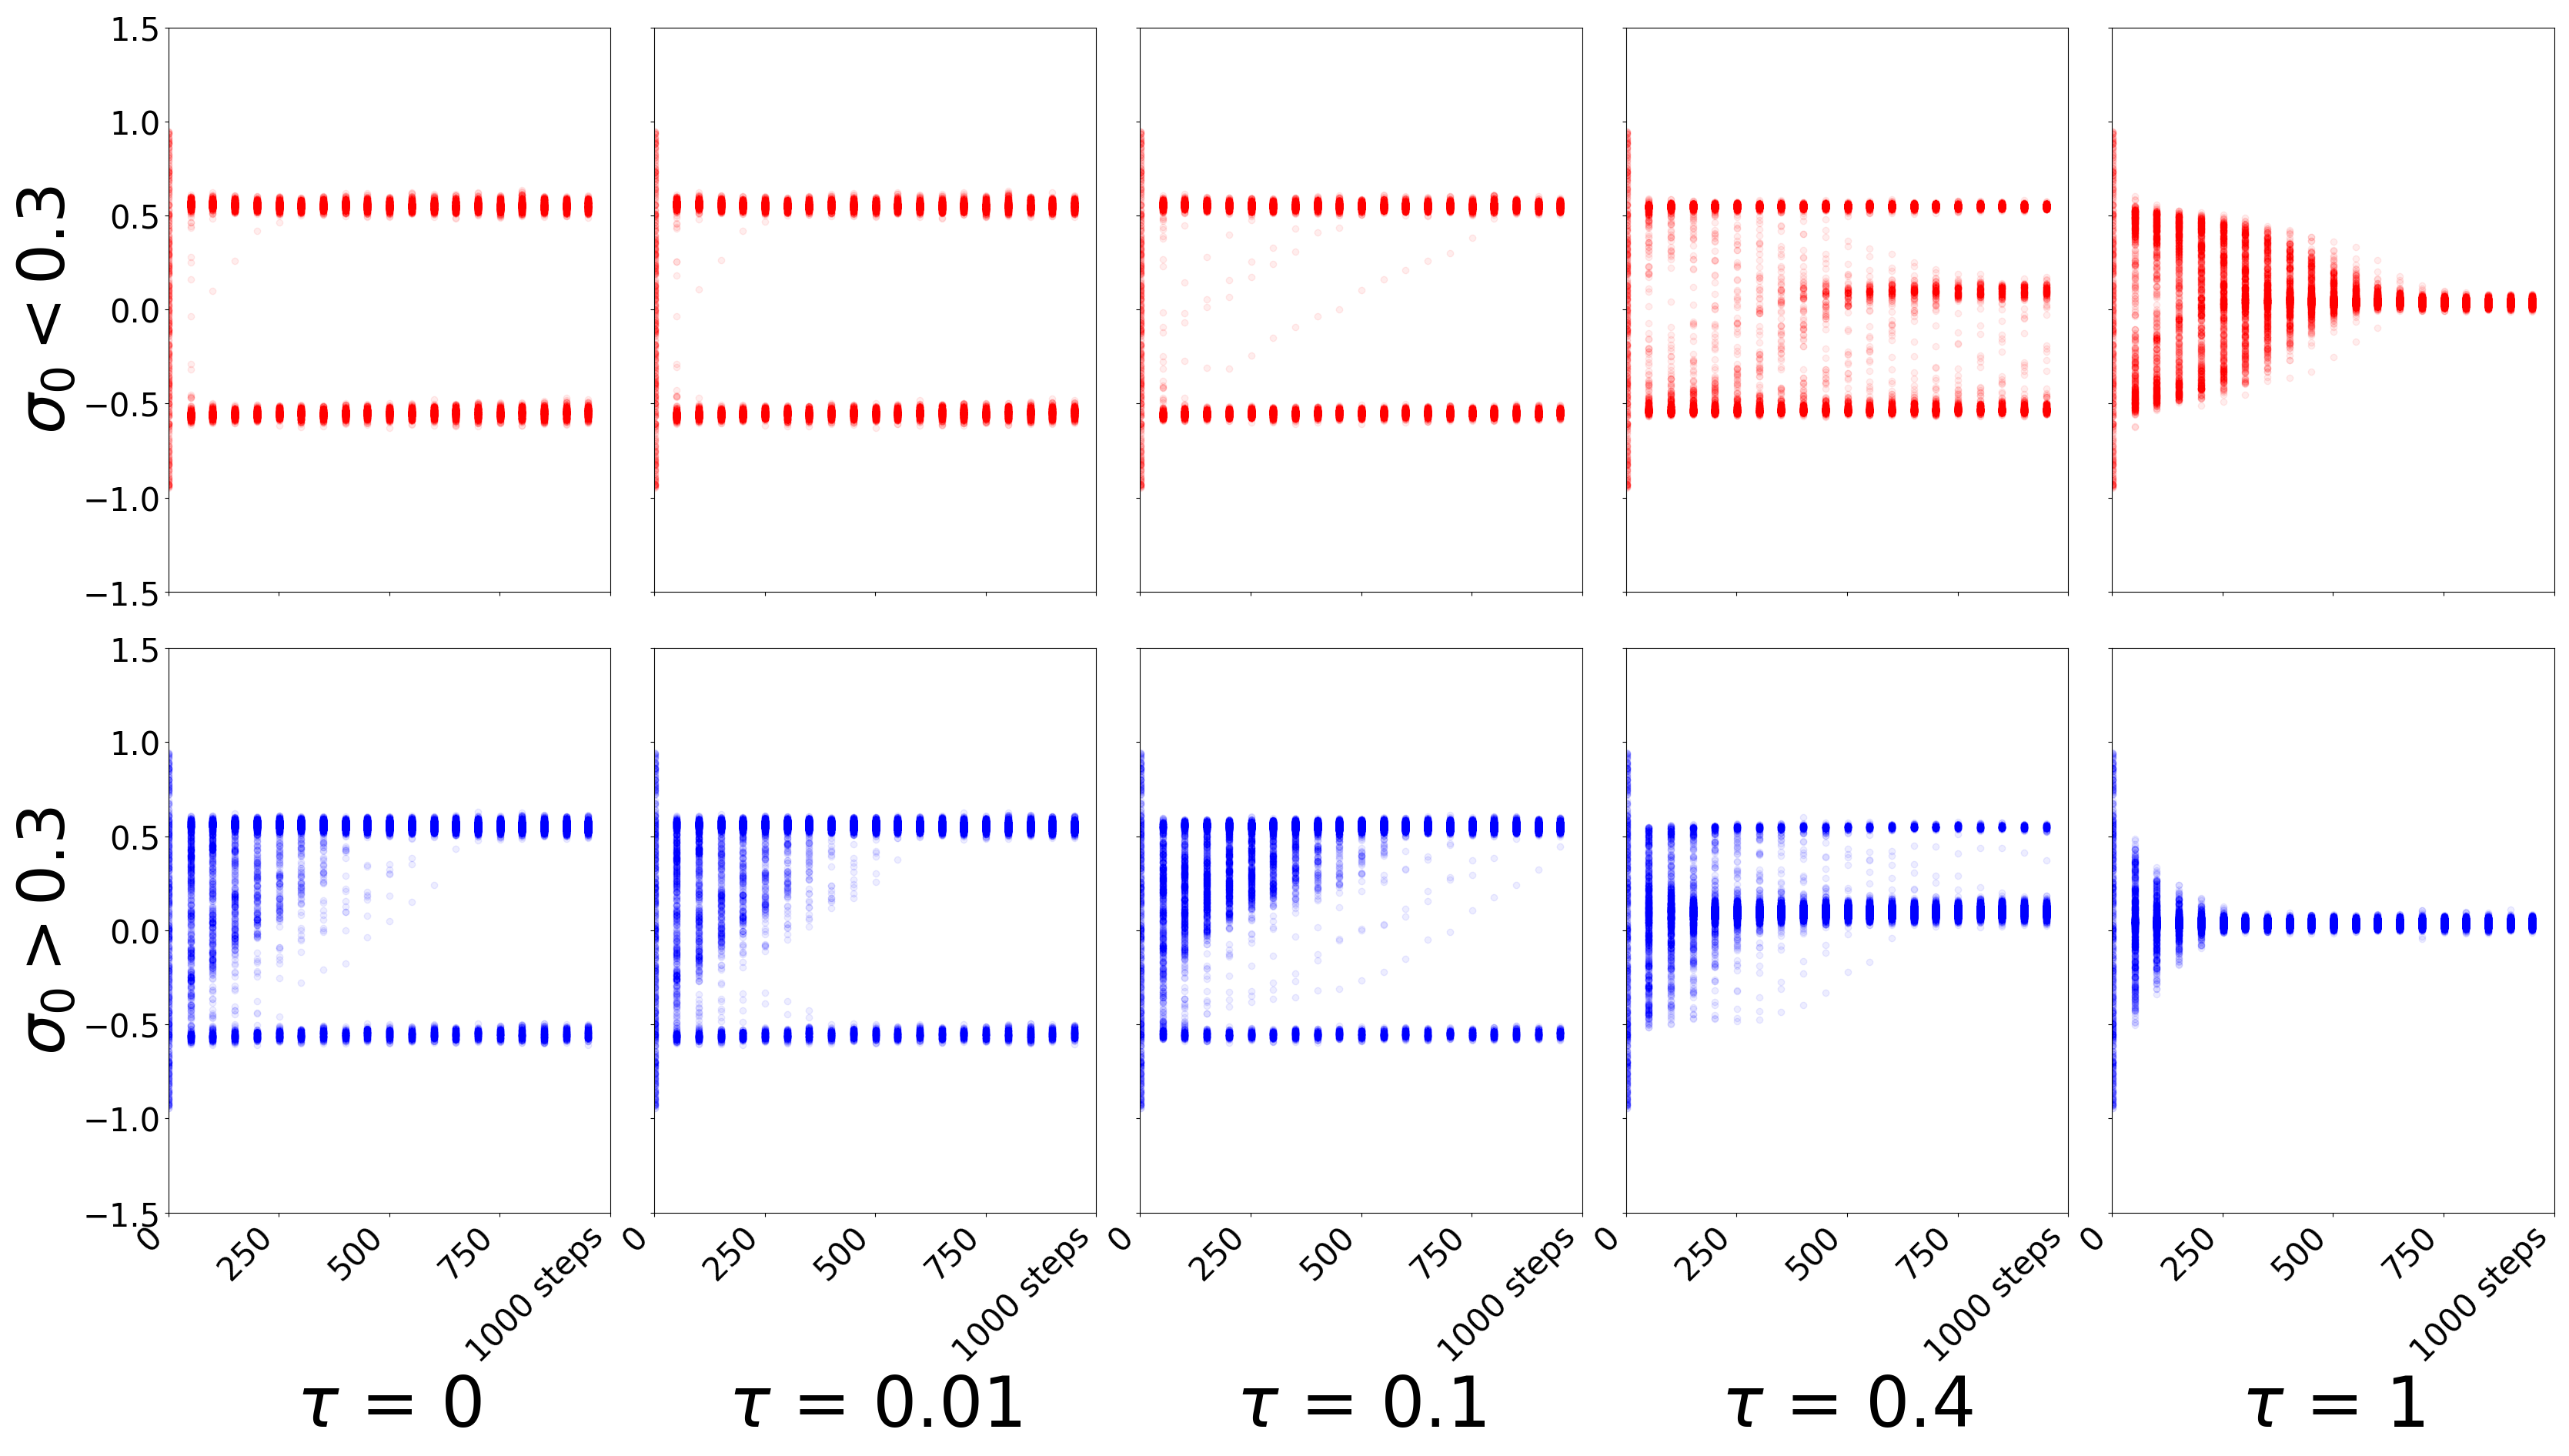
\includegraphics[width=0.8\columnwidth]{figs/bandit/monte-carlo/10/mean_reverse_optim=rmsprop_modes=1_lr=0.005.png}
        \caption{Reverse KL.}
        \label{fig:10-sample-cont-bandit-reverse}
  \end{subfigure}
  \caption{Continuous bandit with 10 sample points, learning rate = 0.005, with RMSprop.}
\end{figure}


% \begin{figure}[!htb]
%   \centering
%   \begin{subfigure}[b]{0.85\linewidth}
%     \centering
%     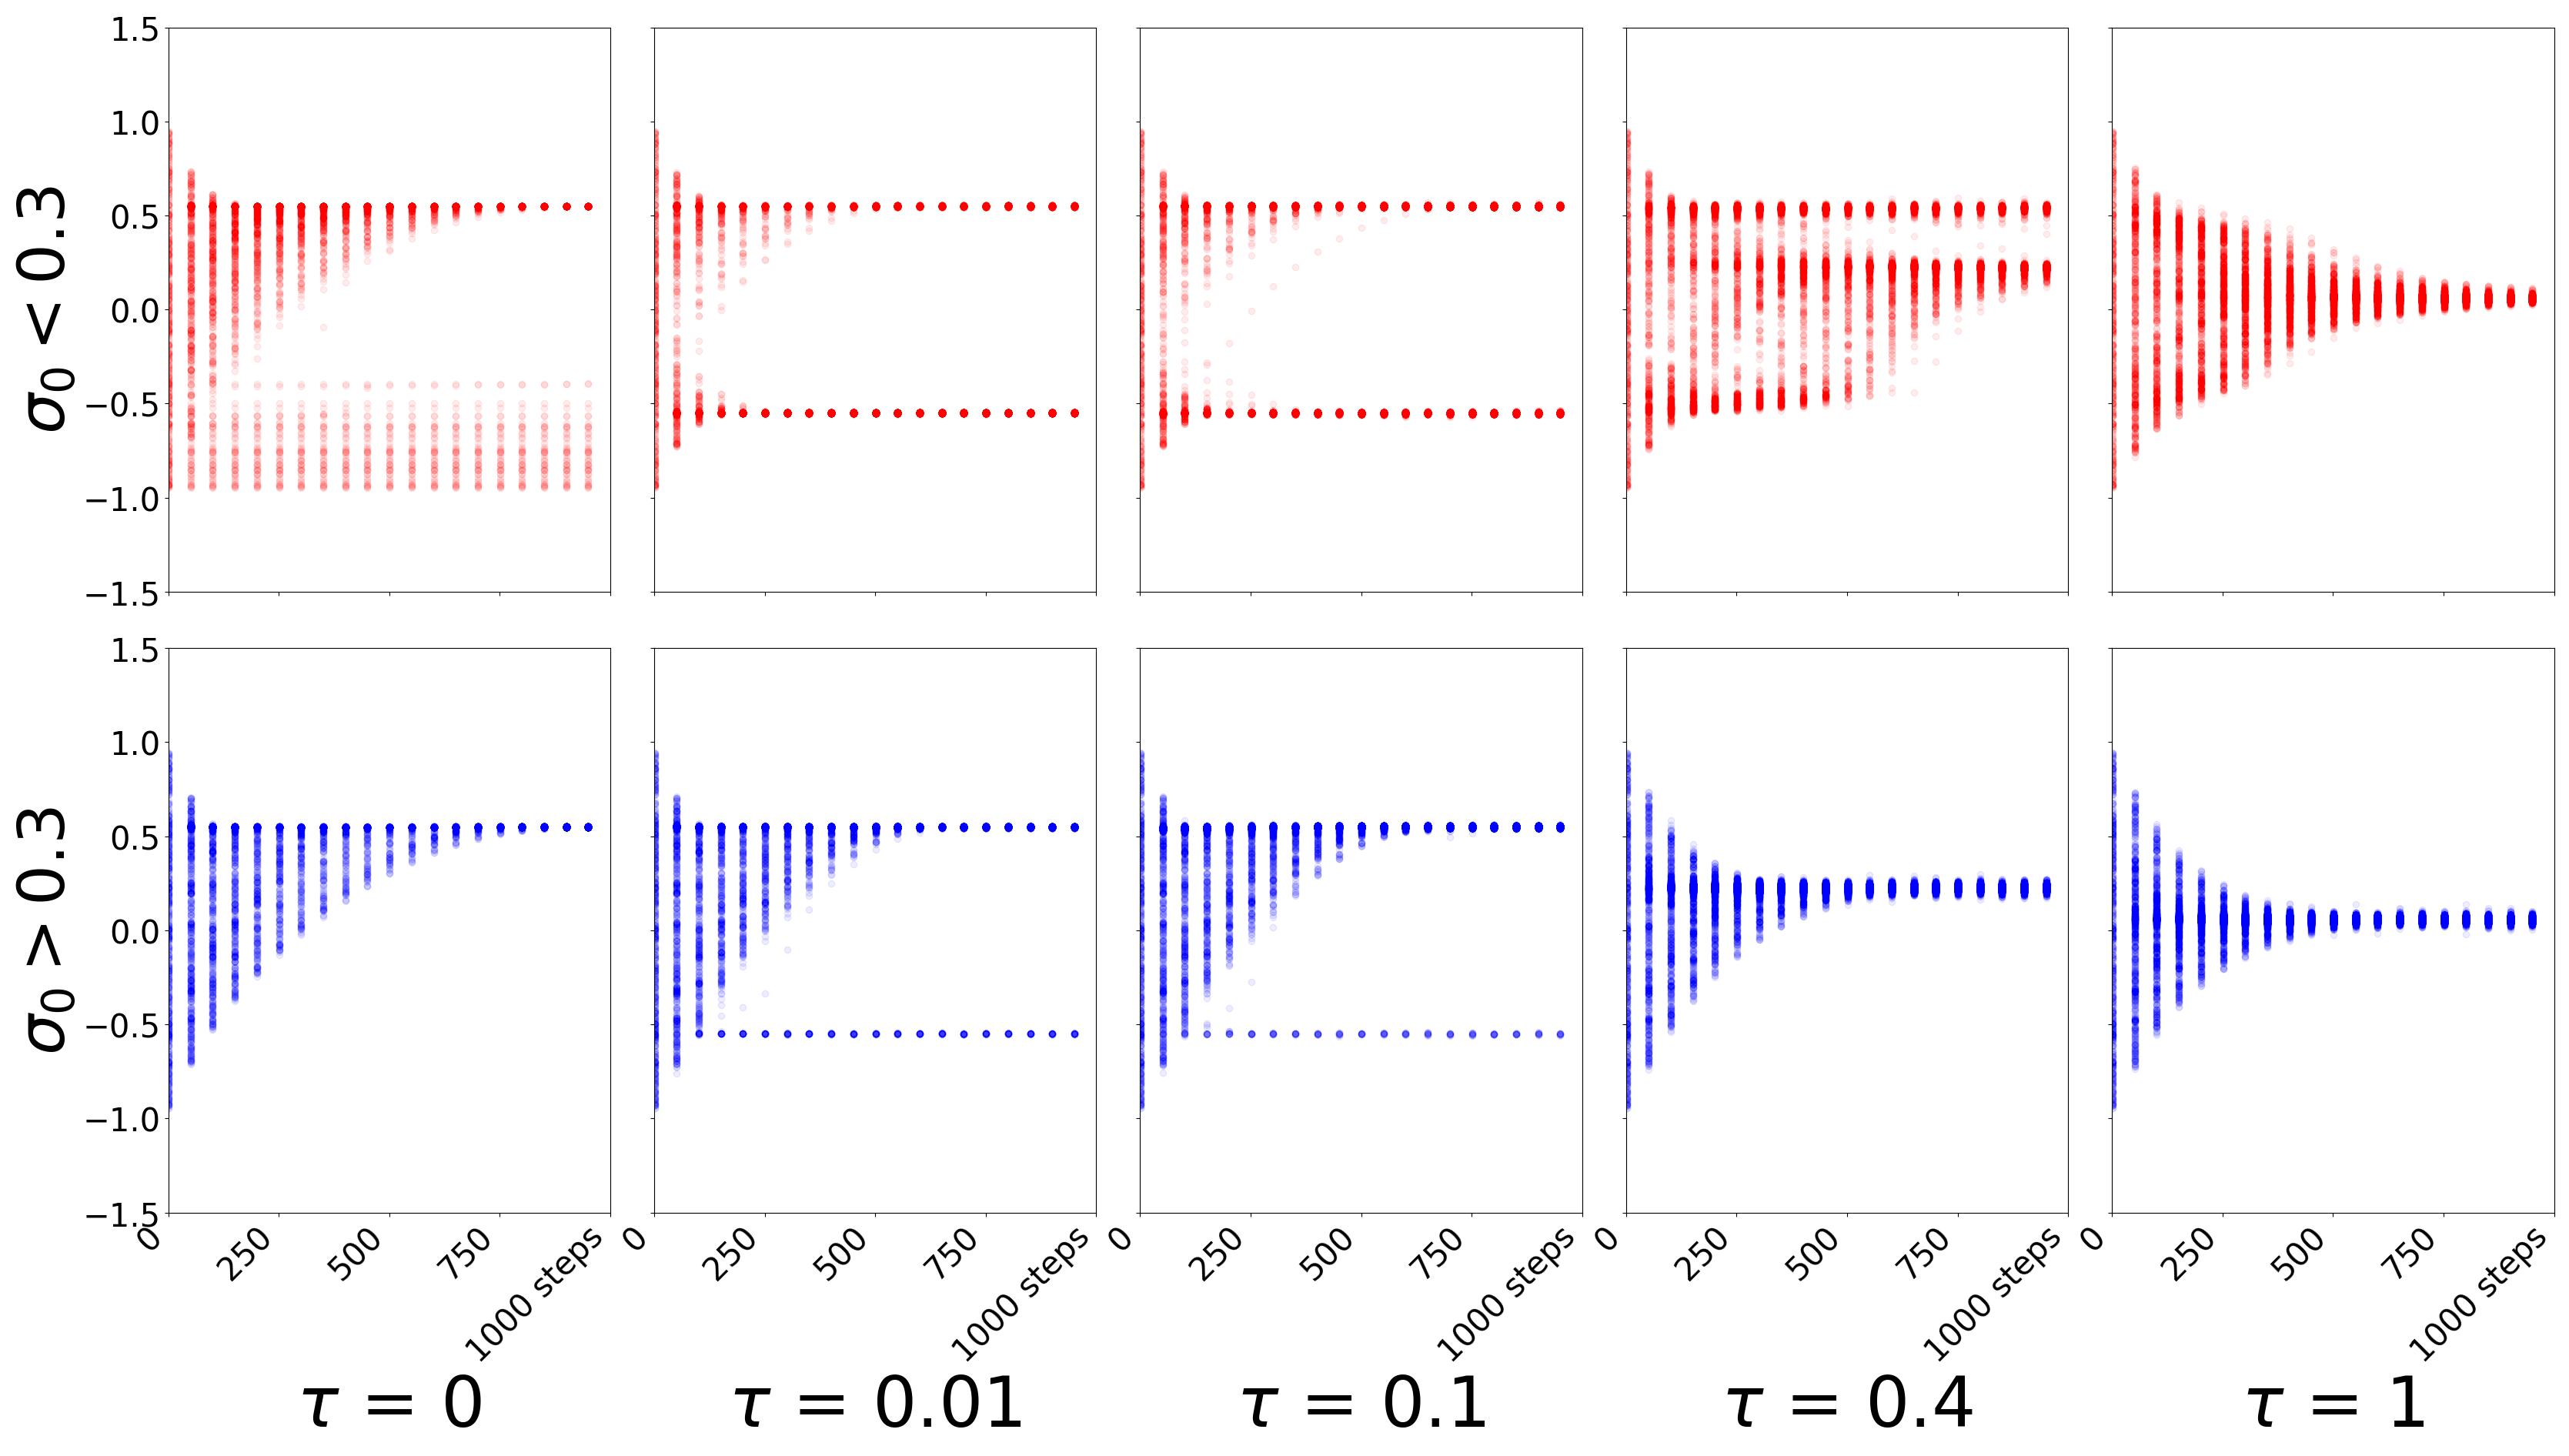
\includegraphics[width=0.8\columnwidth]{figs/bandit/monte-carlo/100/mean_forward_optim=adam_modes=1_lr=0.005.png}
%     \caption{Forward KL.}
%     \label{fig:100-sample-cont-bandit-forward}
%   \end{subfigure}
  
%   \begin{subfigure}[b]{0.85\linewidth}
%         \centering
%         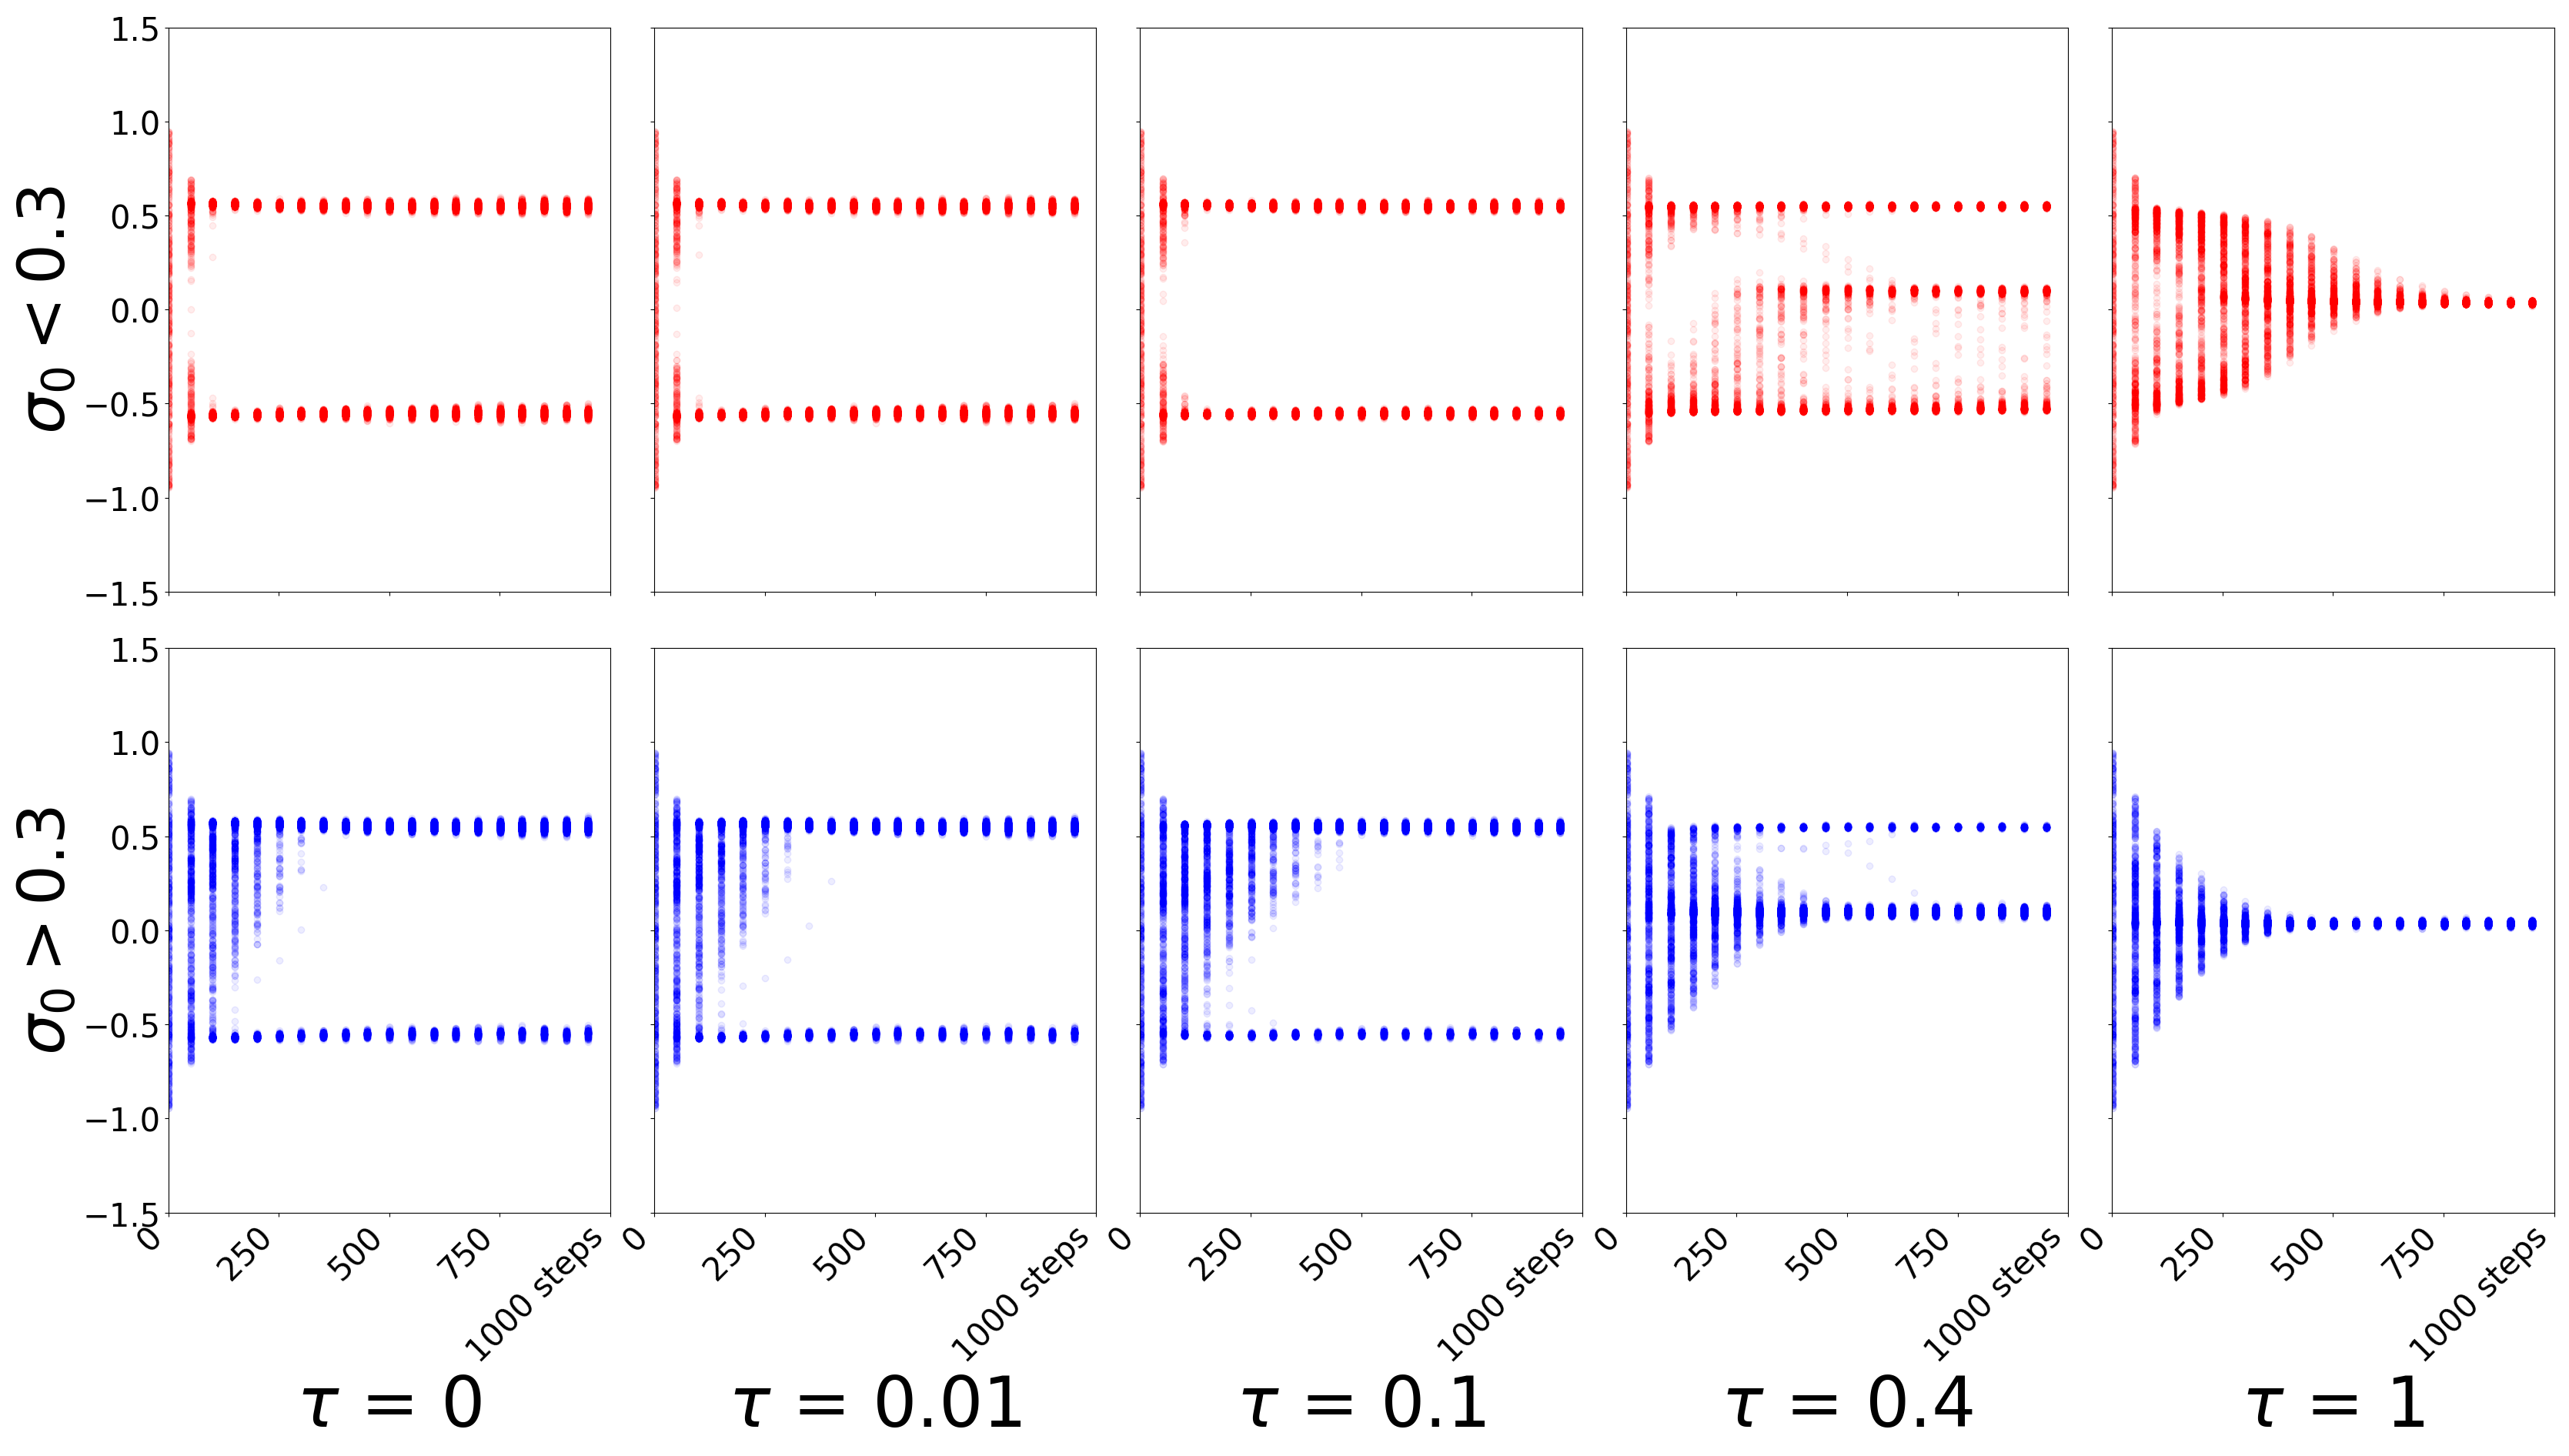
\includegraphics[width=0.8\columnwidth]{figs/bandit/monte-carlo/100/mean_reverse_optim=adam_modes=1_lr=0.005.png}
%         \caption{Reverse KL.}
%         \label{fig:100-sample-cont-bandit-reverse}
%   \end{subfigure}
%   \caption{Continuous bandit with 100 sample points, learning rate = 0.005, with Adam.}
% \end{figure}

% \begin{figure}[!htb]
%   \centering
%   \begin{subfigure}[b]{0.85\linewidth}
%     \centering
%     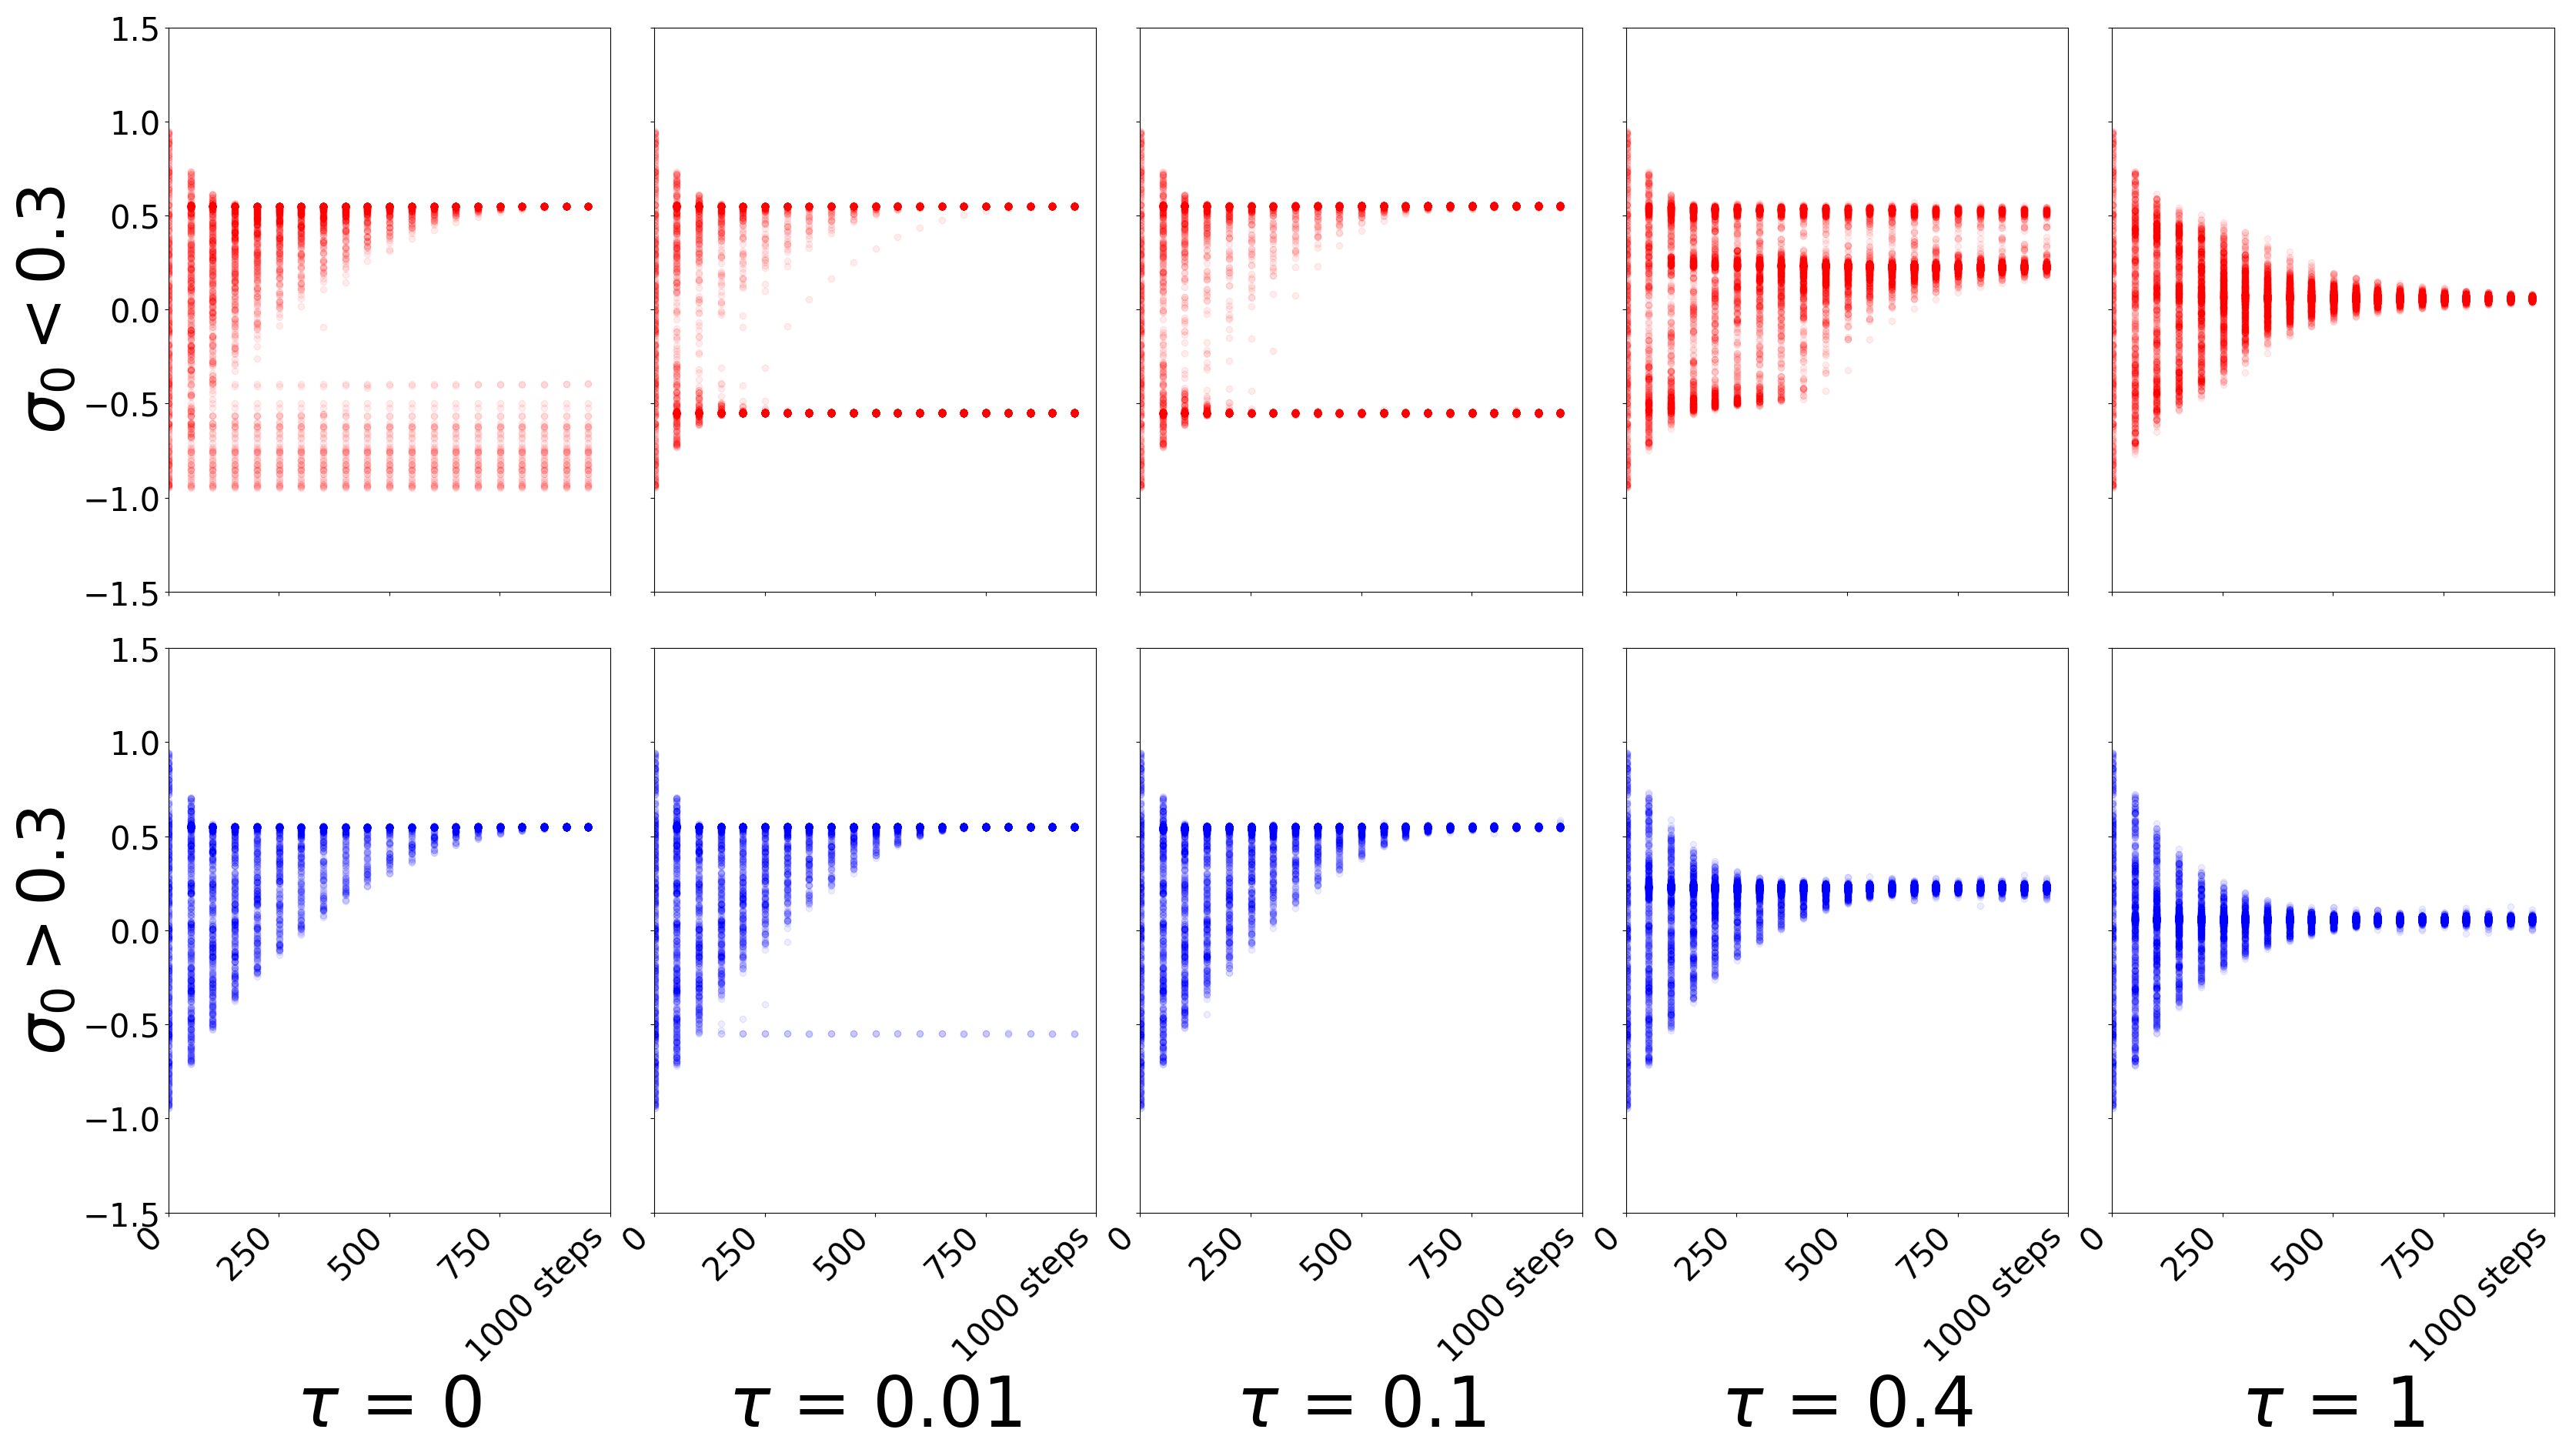
\includegraphics[width=0.8\columnwidth]{figs/bandit/monte-carlo/500/mean_forward_optim=adam_modes=1_lr=0.005.png}
%     \caption{Forward KL.}
%     \label{fig:500-sample-cont-bandit-forward}
%   \end{subfigure}
  
%   \begin{subfigure}[b]{0.85\linewidth}
%         \centering
%         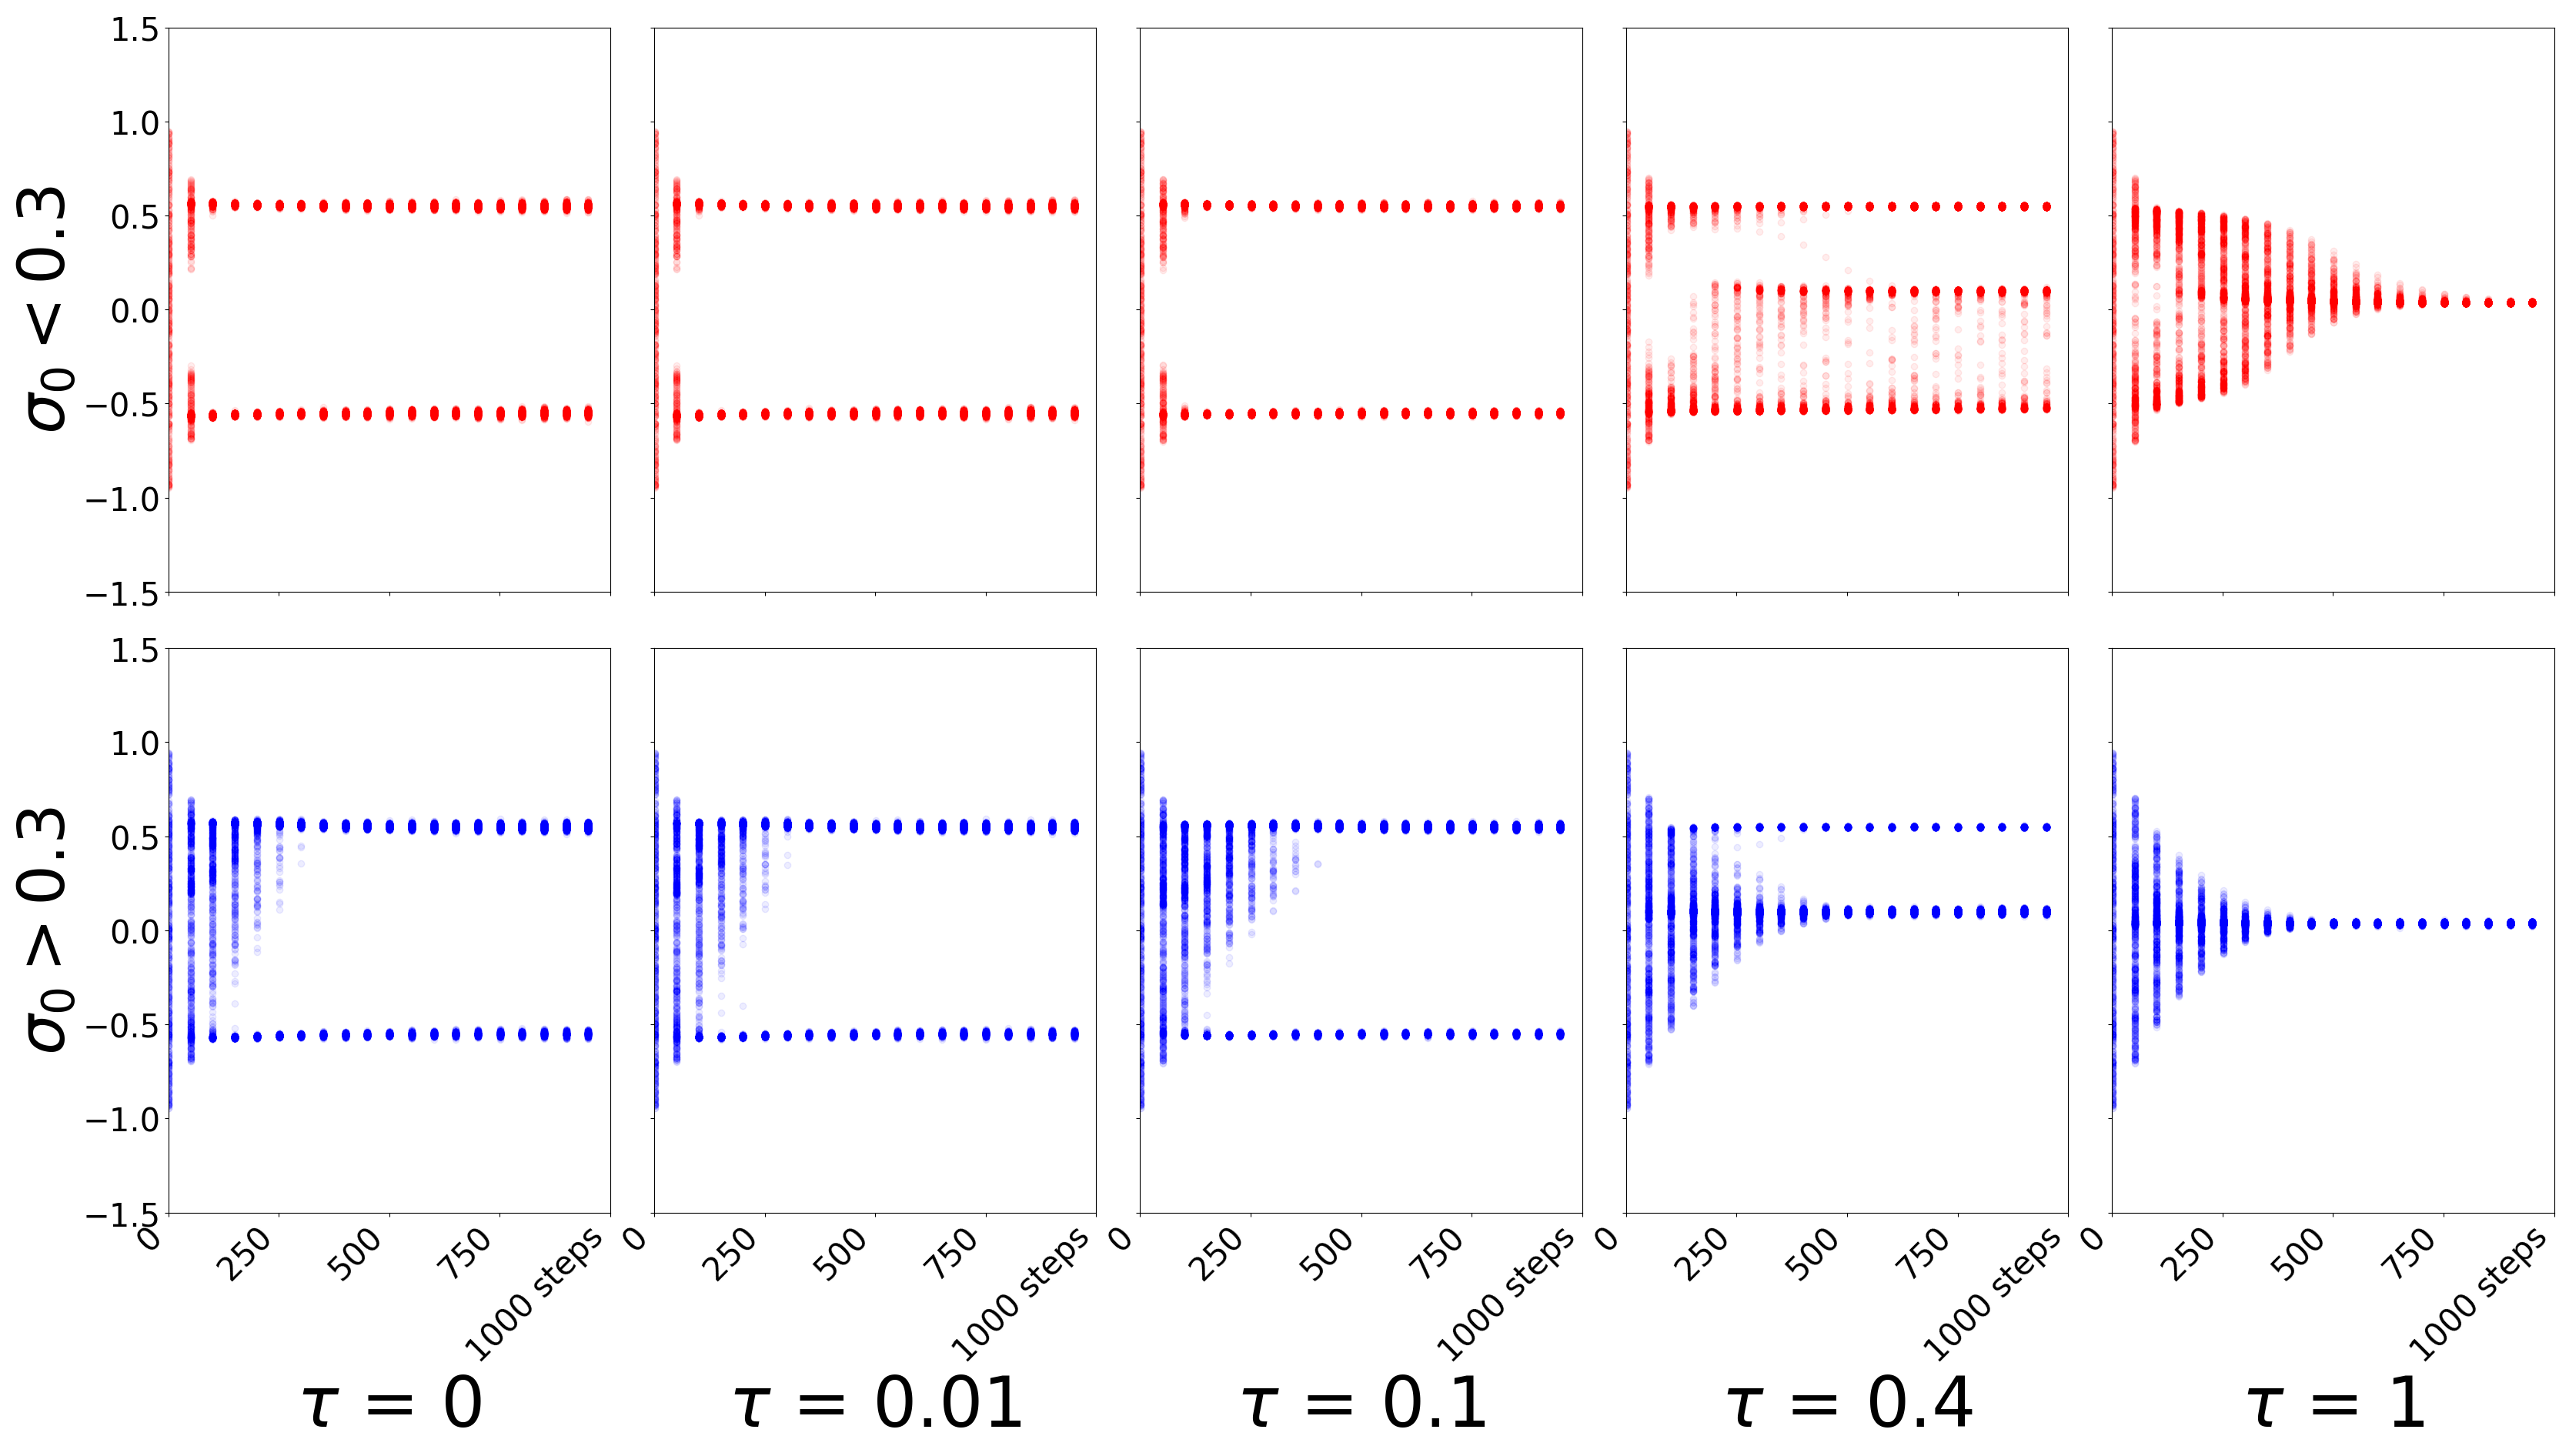
\includegraphics[width=0.8\columnwidth]{figs/bandit/monte-carlo/500/mean_reverse_optim=adam_modes=1_lr=0.005.png}
%         \caption{Reverse KL.}
%         \label{fig:500-sample-cont-bandit-reverse}
%   \end{subfigure}
%   \caption{Continuous bandit with 500 sample points, learning rate = 0.005, with Adam.}
% \end{figure}


\begin{figure}[!htb]
  \centering
  \begin{subfigure}[b]{0.85\linewidth}
    \centering
    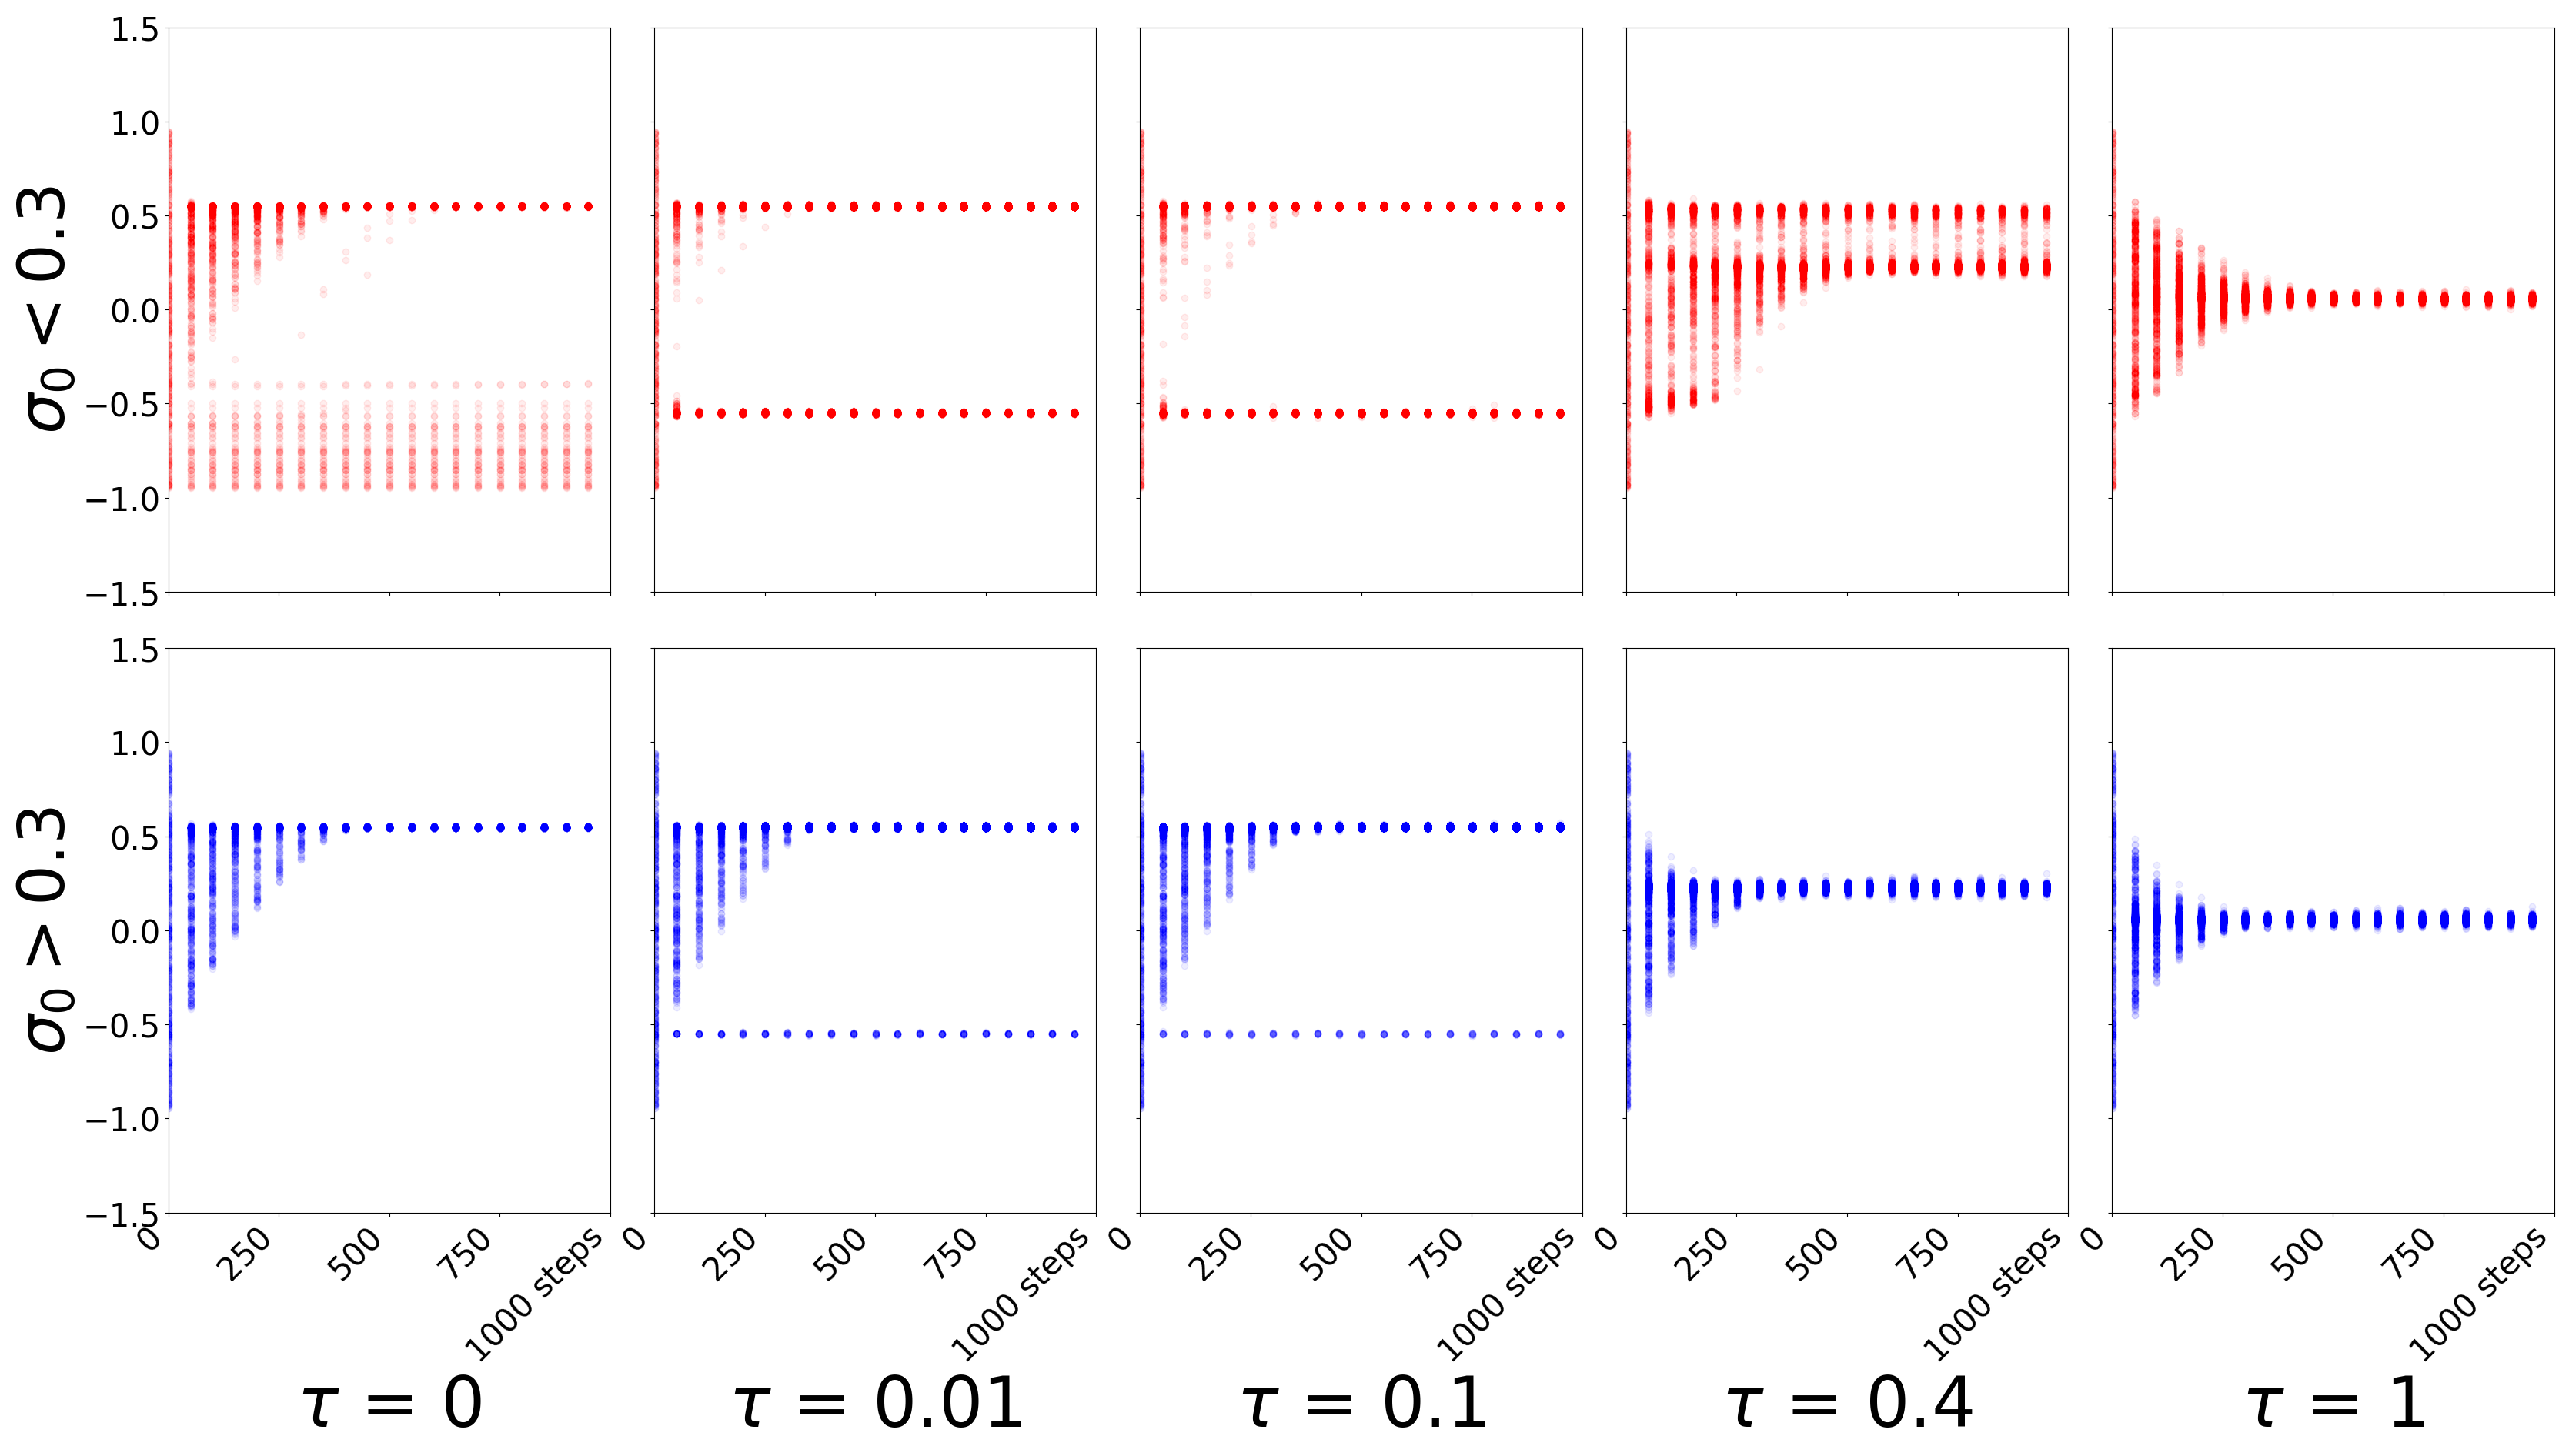
\includegraphics[width=0.8\columnwidth]{figs/bandit/monte-carlo/500/mean_forward_optim=rmsprop_modes=1_lr=0.005.png}
    \caption{Forward KL.}
    \label{fig:500-sample-cont-bandit-forward}
  \end{subfigure}
  
  \begin{subfigure}[b]{0.85\linewidth}
        \centering
        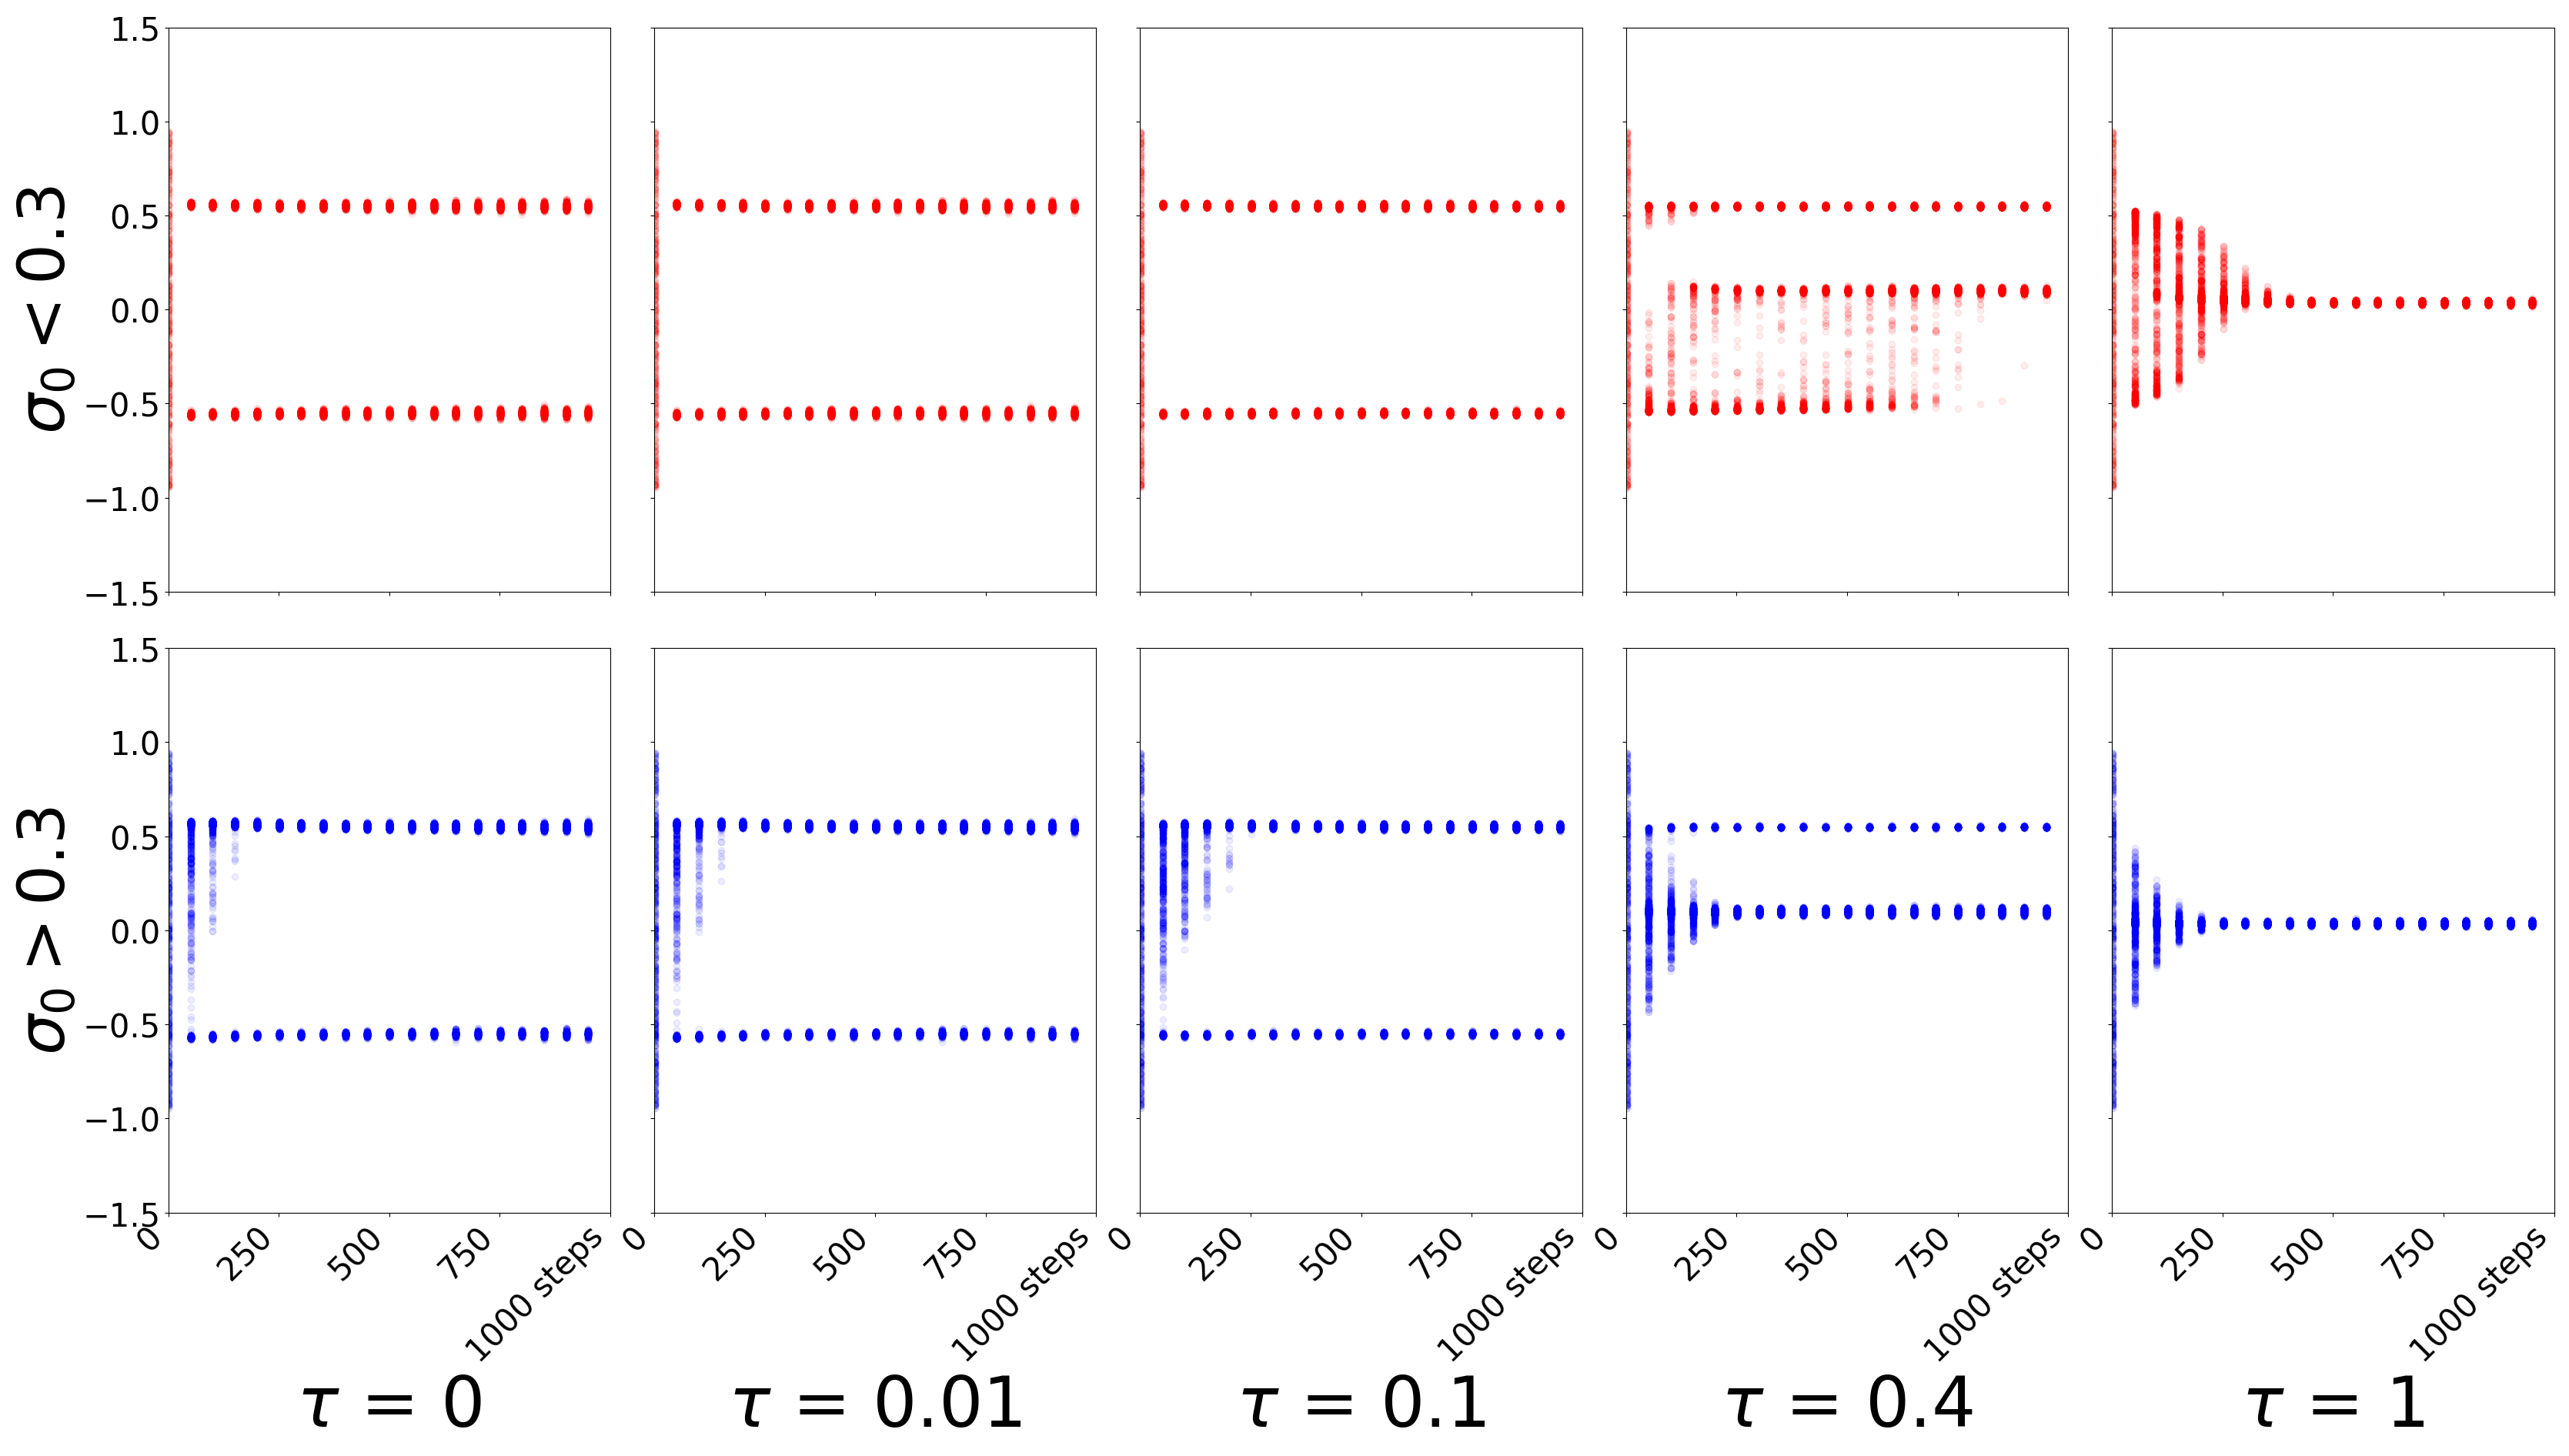
\includegraphics[width=0.8\columnwidth]{figs/bandit/monte-carlo/500/mean_reverse_optim=rmsprop_modes=1_lr=0.005.png}
        \caption{Reverse KL.}
        \label{fig:500-sample-cont-bandit-reverse}
  \end{subfigure}
  \caption{Continuous bandit with 500 sample points, learning rate = 0.005, with RMSprop.}
\end{figure}


While overall behaviour for the continuous bandit is consistent with the results using Clenshaw-Curtis quadrature, the iterates seem to cluster more slowly around their limit points, or not at all. 
% \textbf{Switch-Stay}

% \begin{figure}[!htb]
%   \centering
%   \begin{subfigure}[b]{0.85\linewidth}
%     \centering
%     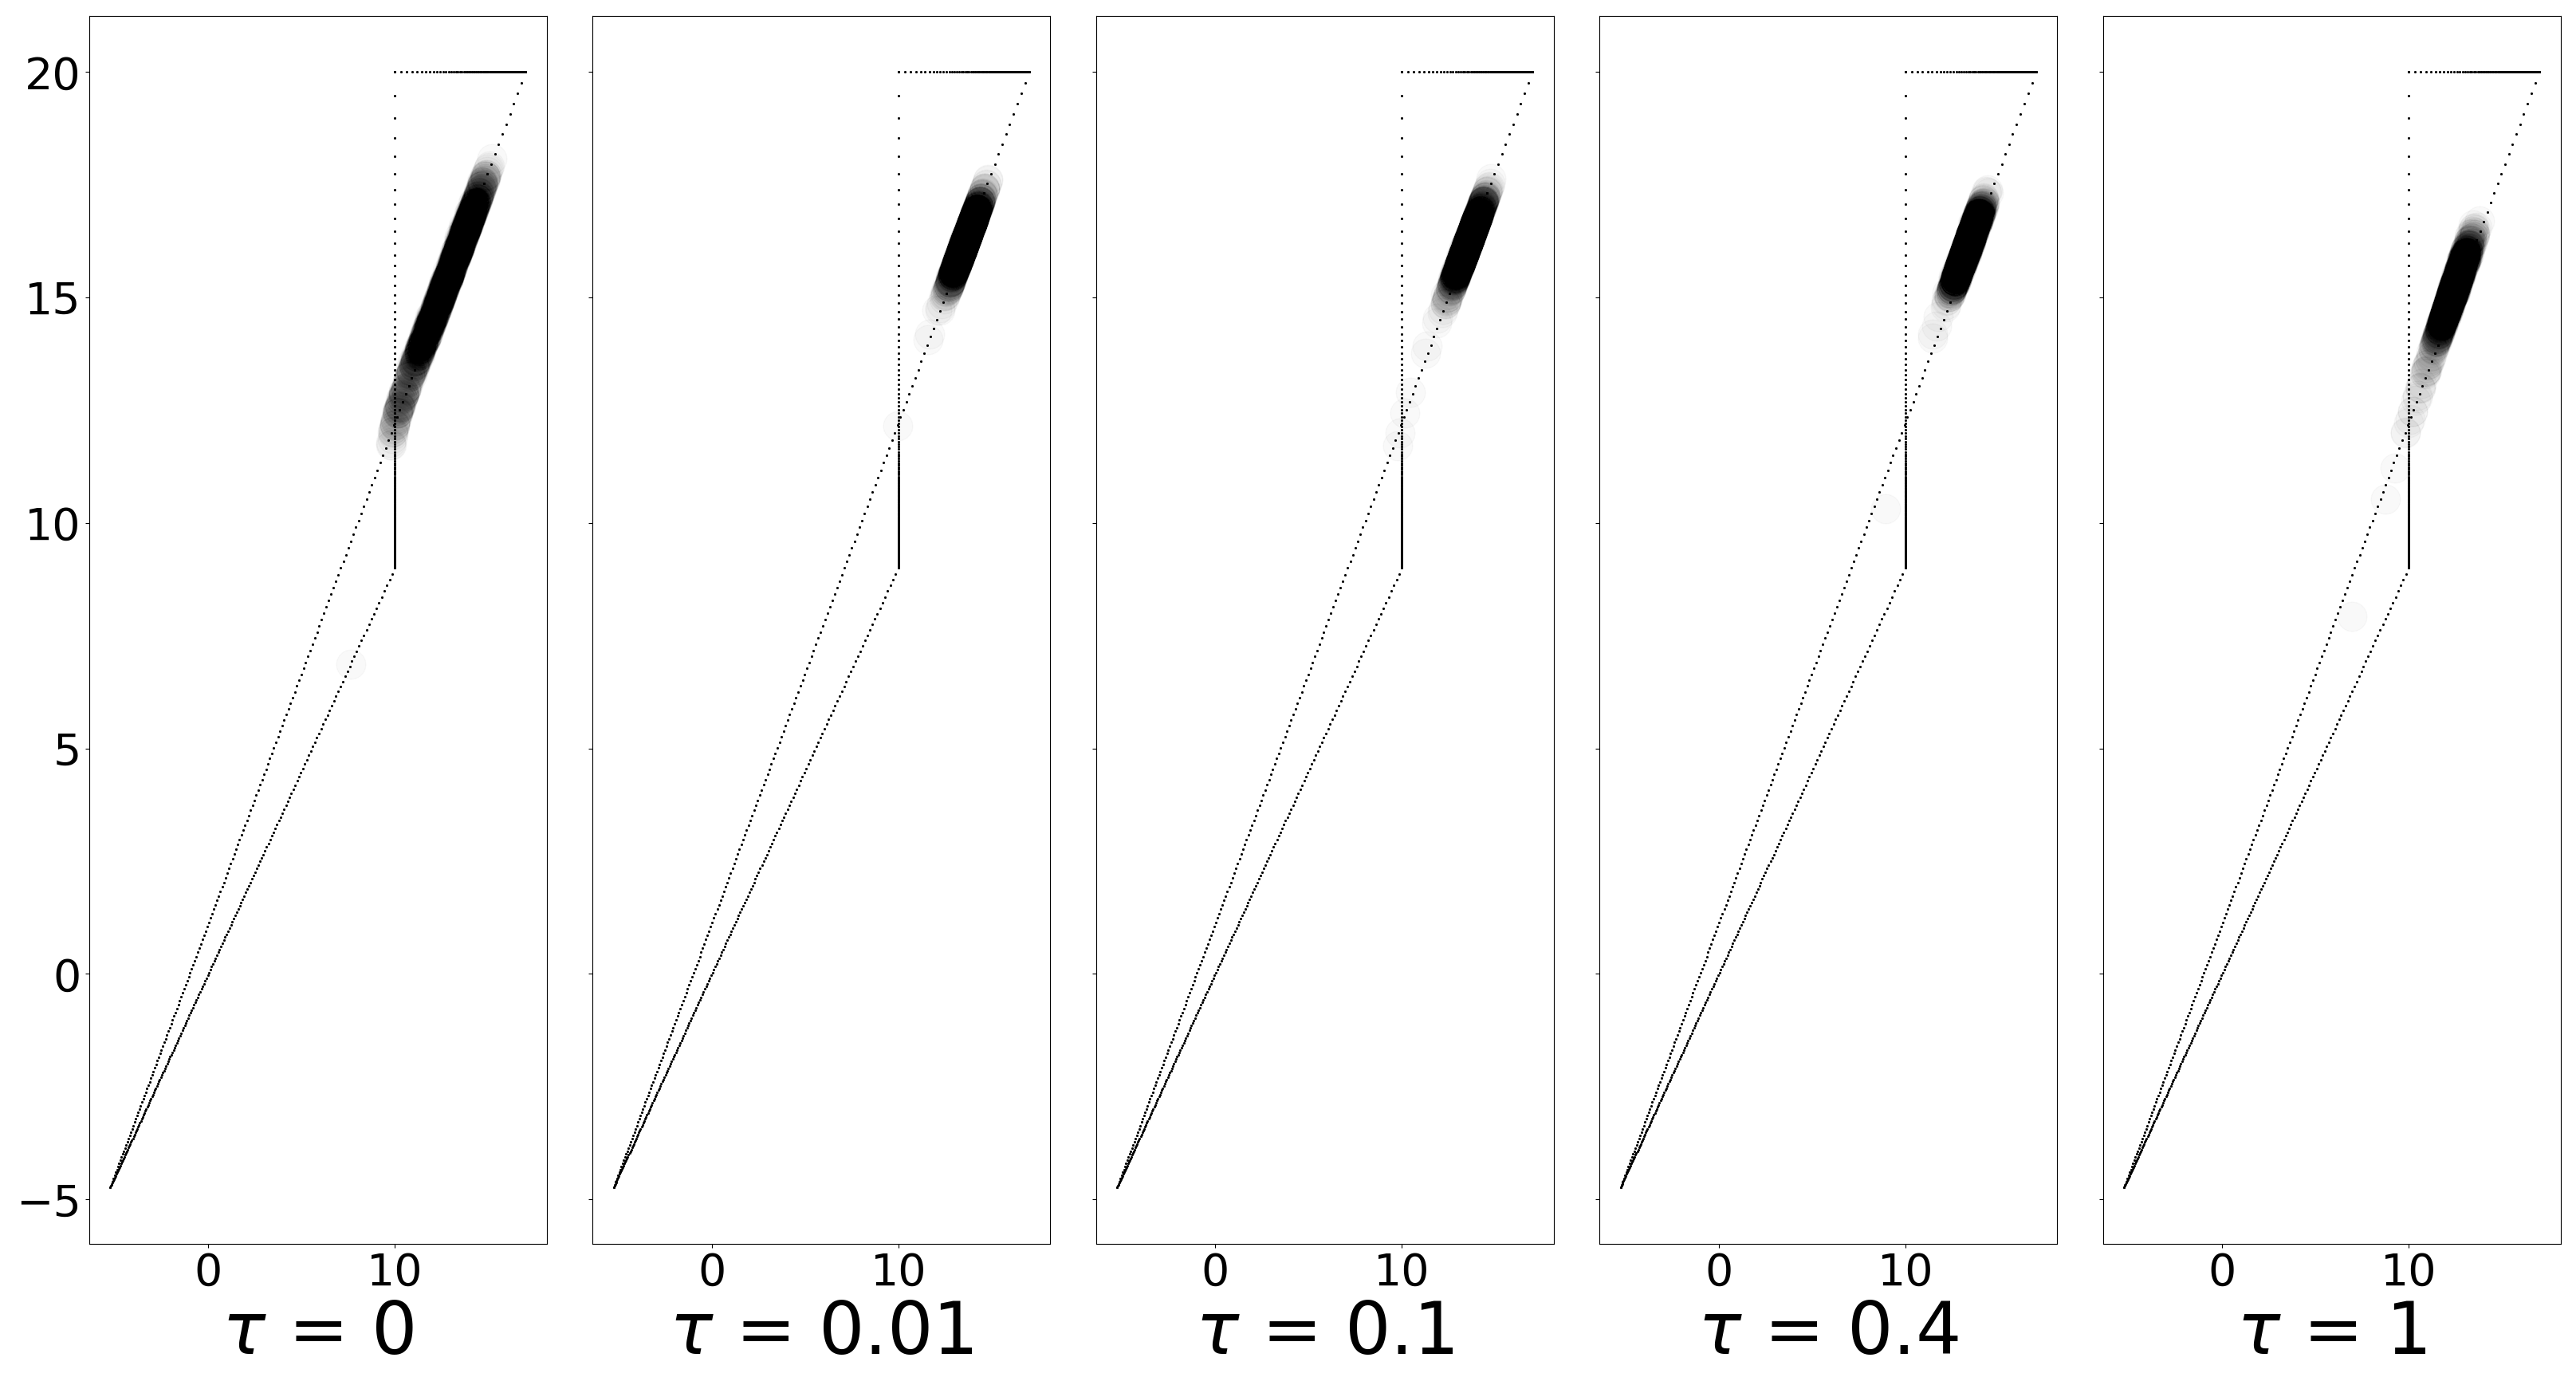
\includegraphics[width=0.8\columnwidth]{figs/continuous-switch-stay/monte-carlo/10/polytope_forward_optim=adam_lr=0.01.png}
%     \caption{Forward KL.}
%     \label{fig:10-sample-switch-stay-forward}
%   \end{subfigure}
  
%   \begin{subfigure}[b]{0.85\linewidth}
%         \centering
%         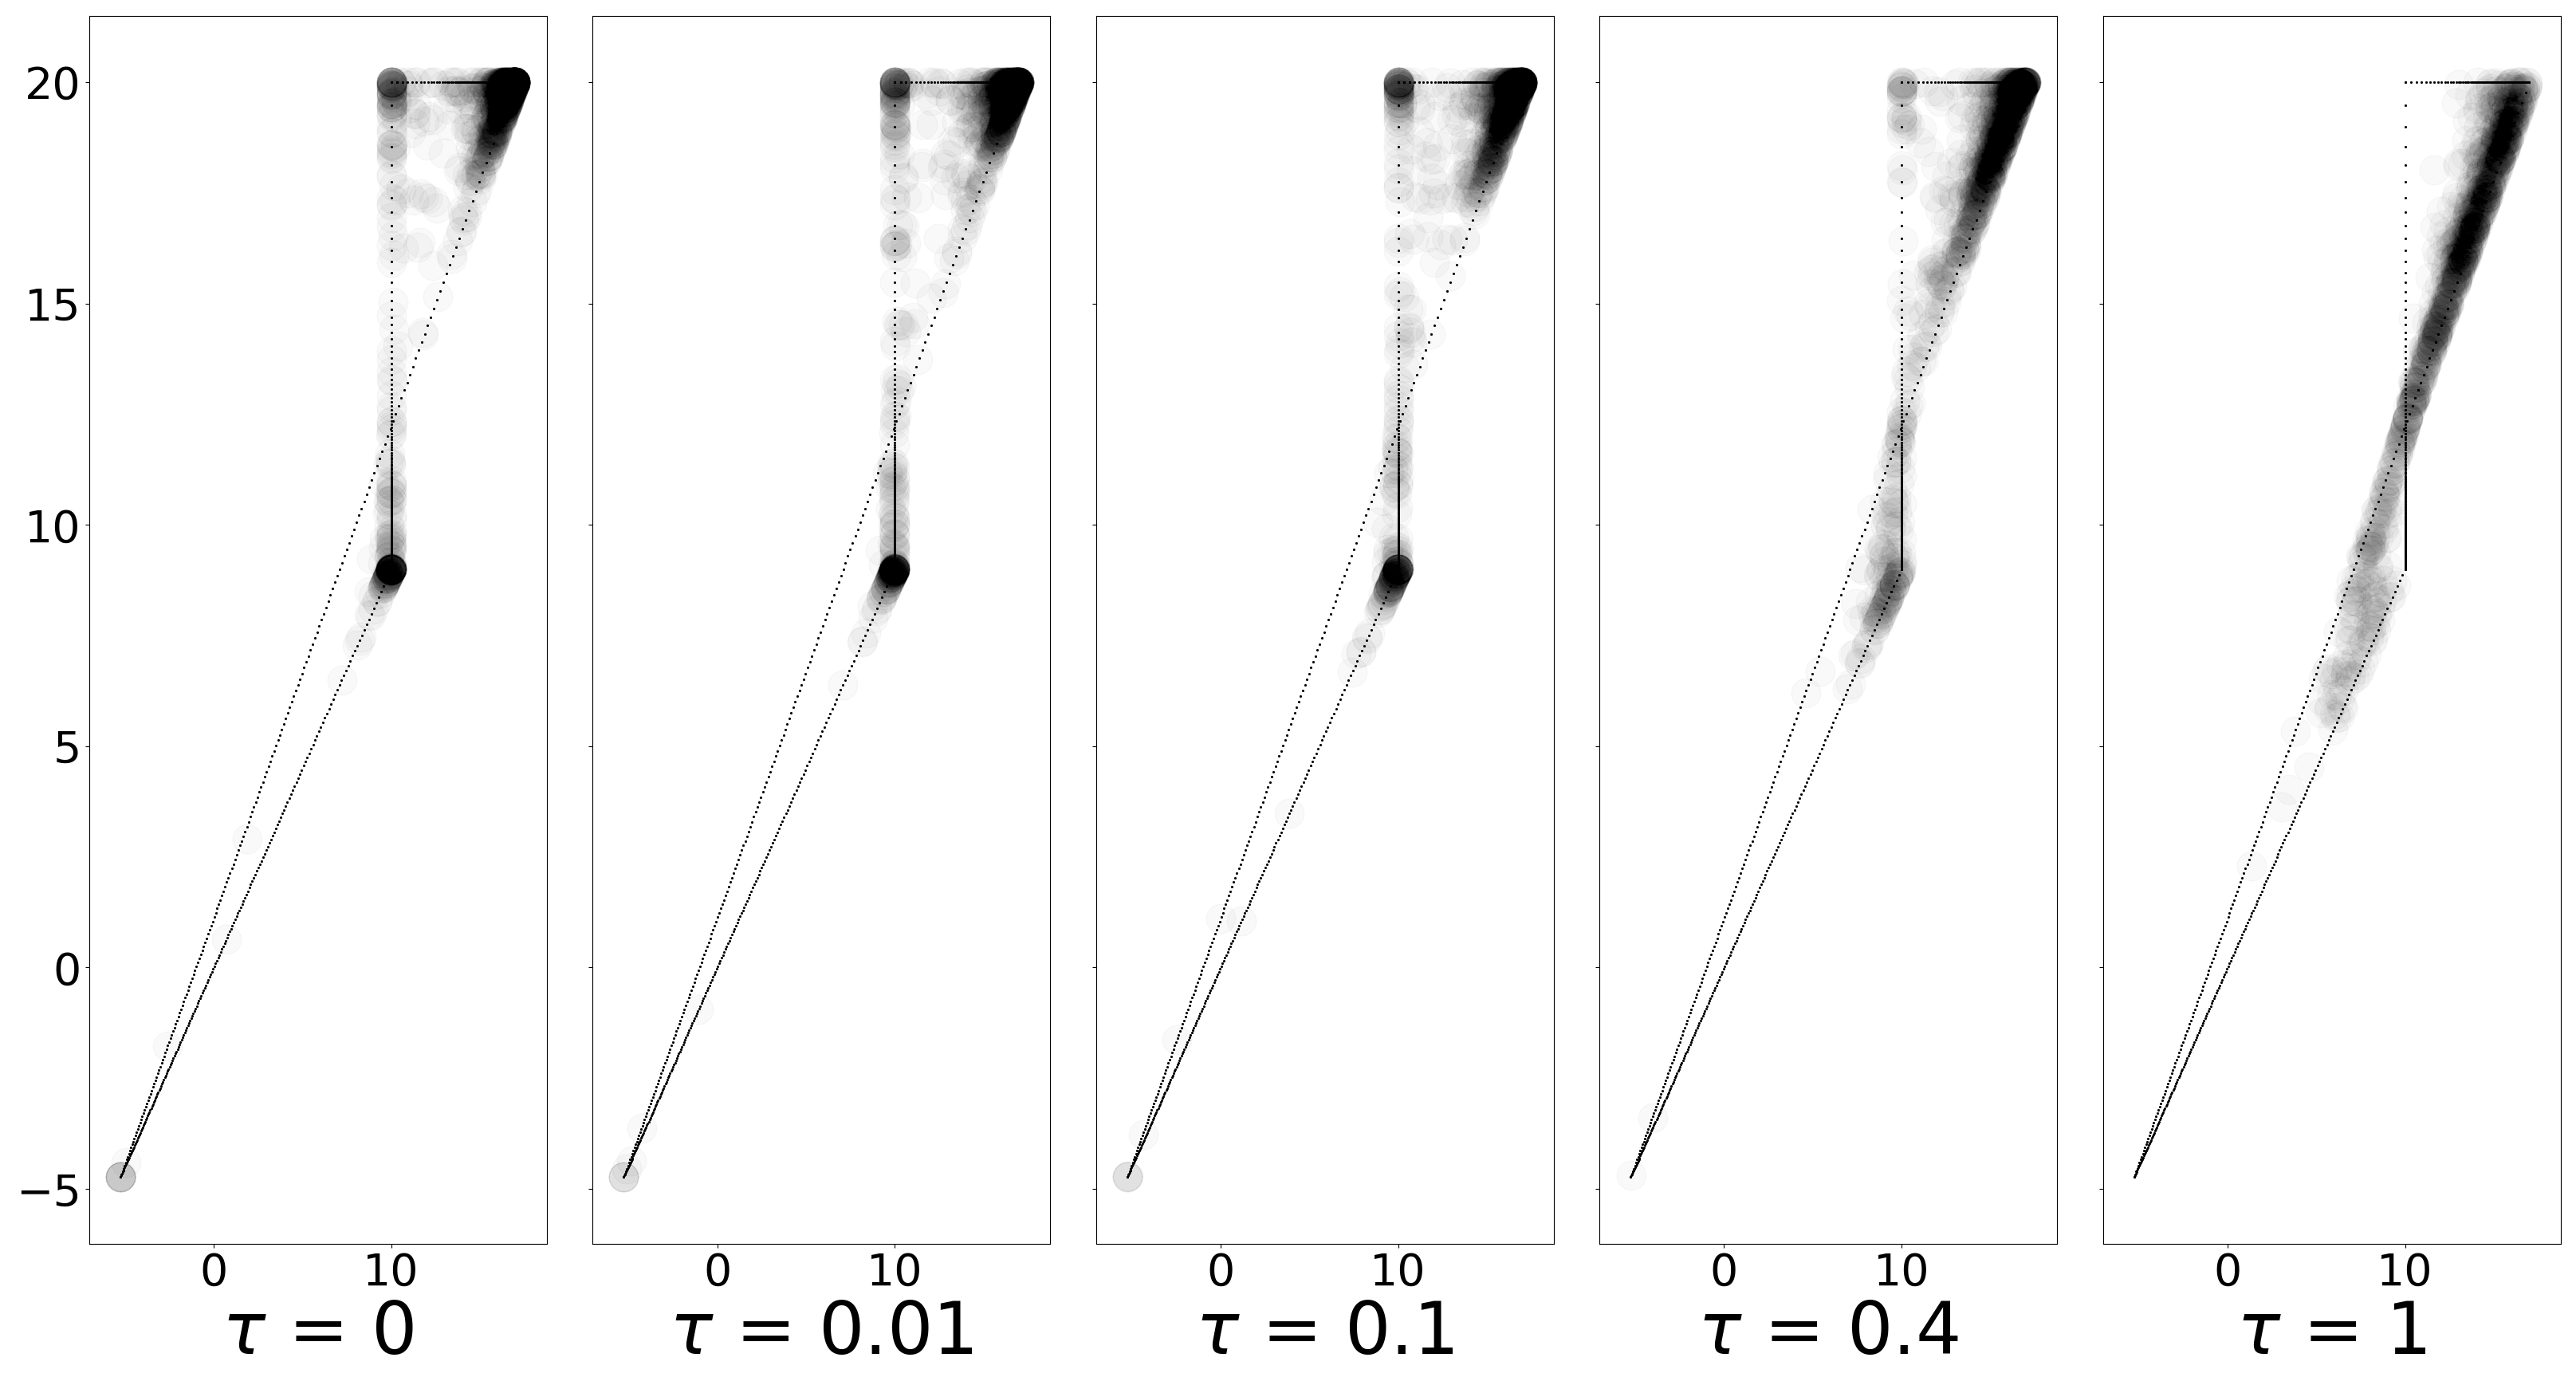
\includegraphics[width=0.8\columnwidth]{figs/continuous-switch-stay/monte-carlo/10/polytope_reverse_optim=adam_lr=0.01.png}
%         \caption{Reverse KL.}
%         \label{fig:10-sample-switch-stay-reverse}
%   \end{subfigure}
%   \caption{Switch-stay with 10 sample points, learning rate = 0.01, with Adam.}
% \end{figure}

\begin{figure}[!htb]
  \centering
  \begin{subfigure}[b]{0.85\linewidth}
    \centering
    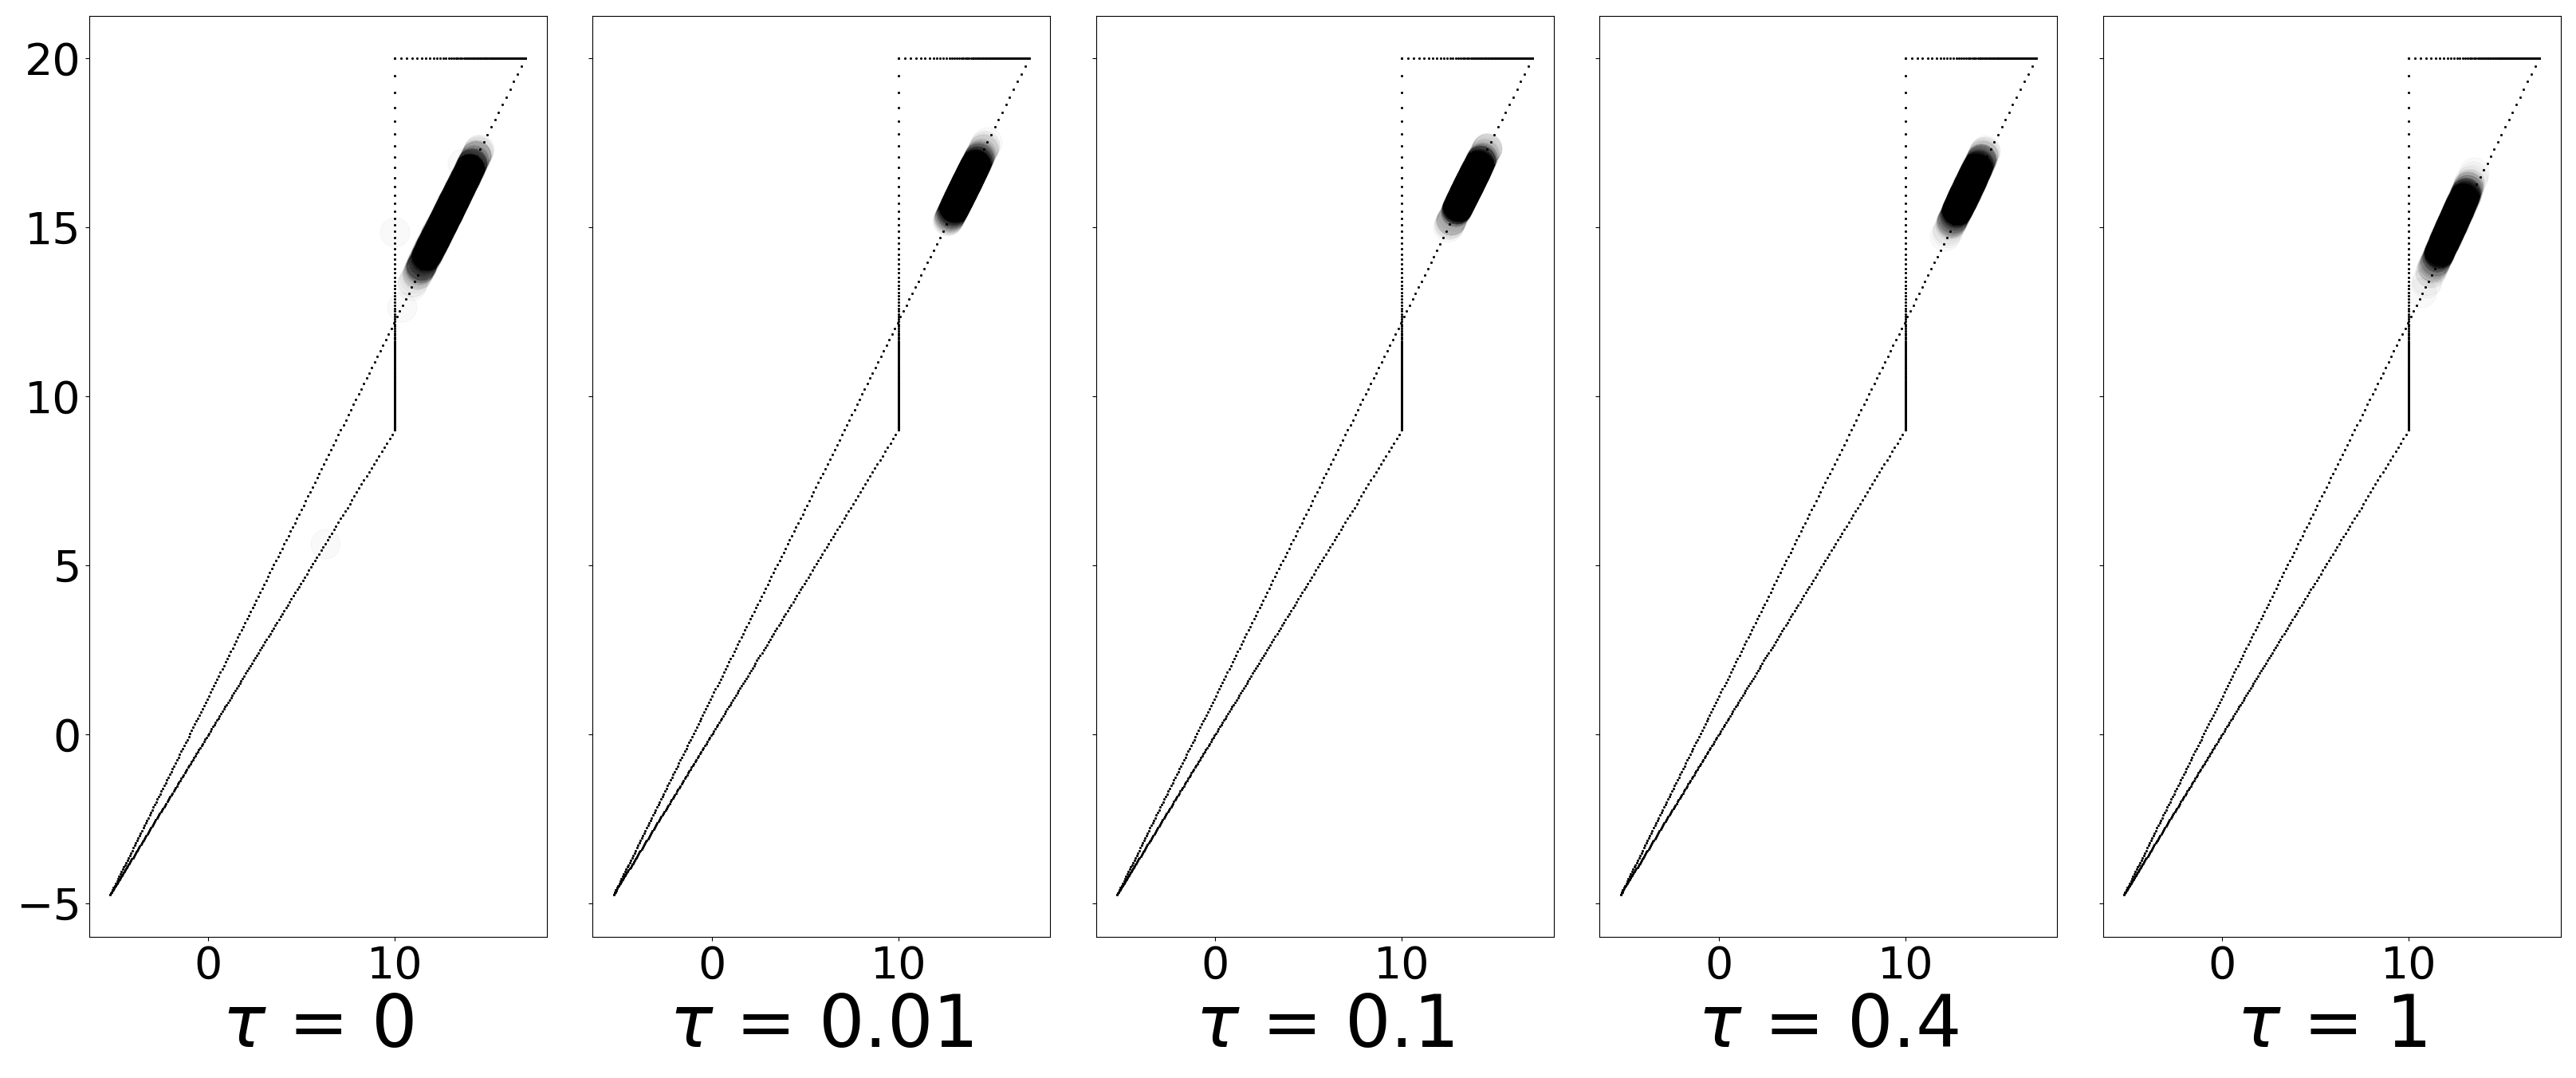
\includegraphics[width=0.8\columnwidth]{figs/continuous-switch-stay/monte-carlo/10/polytope_forward_optim=rmsprop_lr=0.01.png}
    \caption{Forward KL.}
    \label{fig:10-sample-switch-stay-forward}
  \end{subfigure}
  
  \begin{subfigure}[b]{0.85\linewidth}
        \centering
        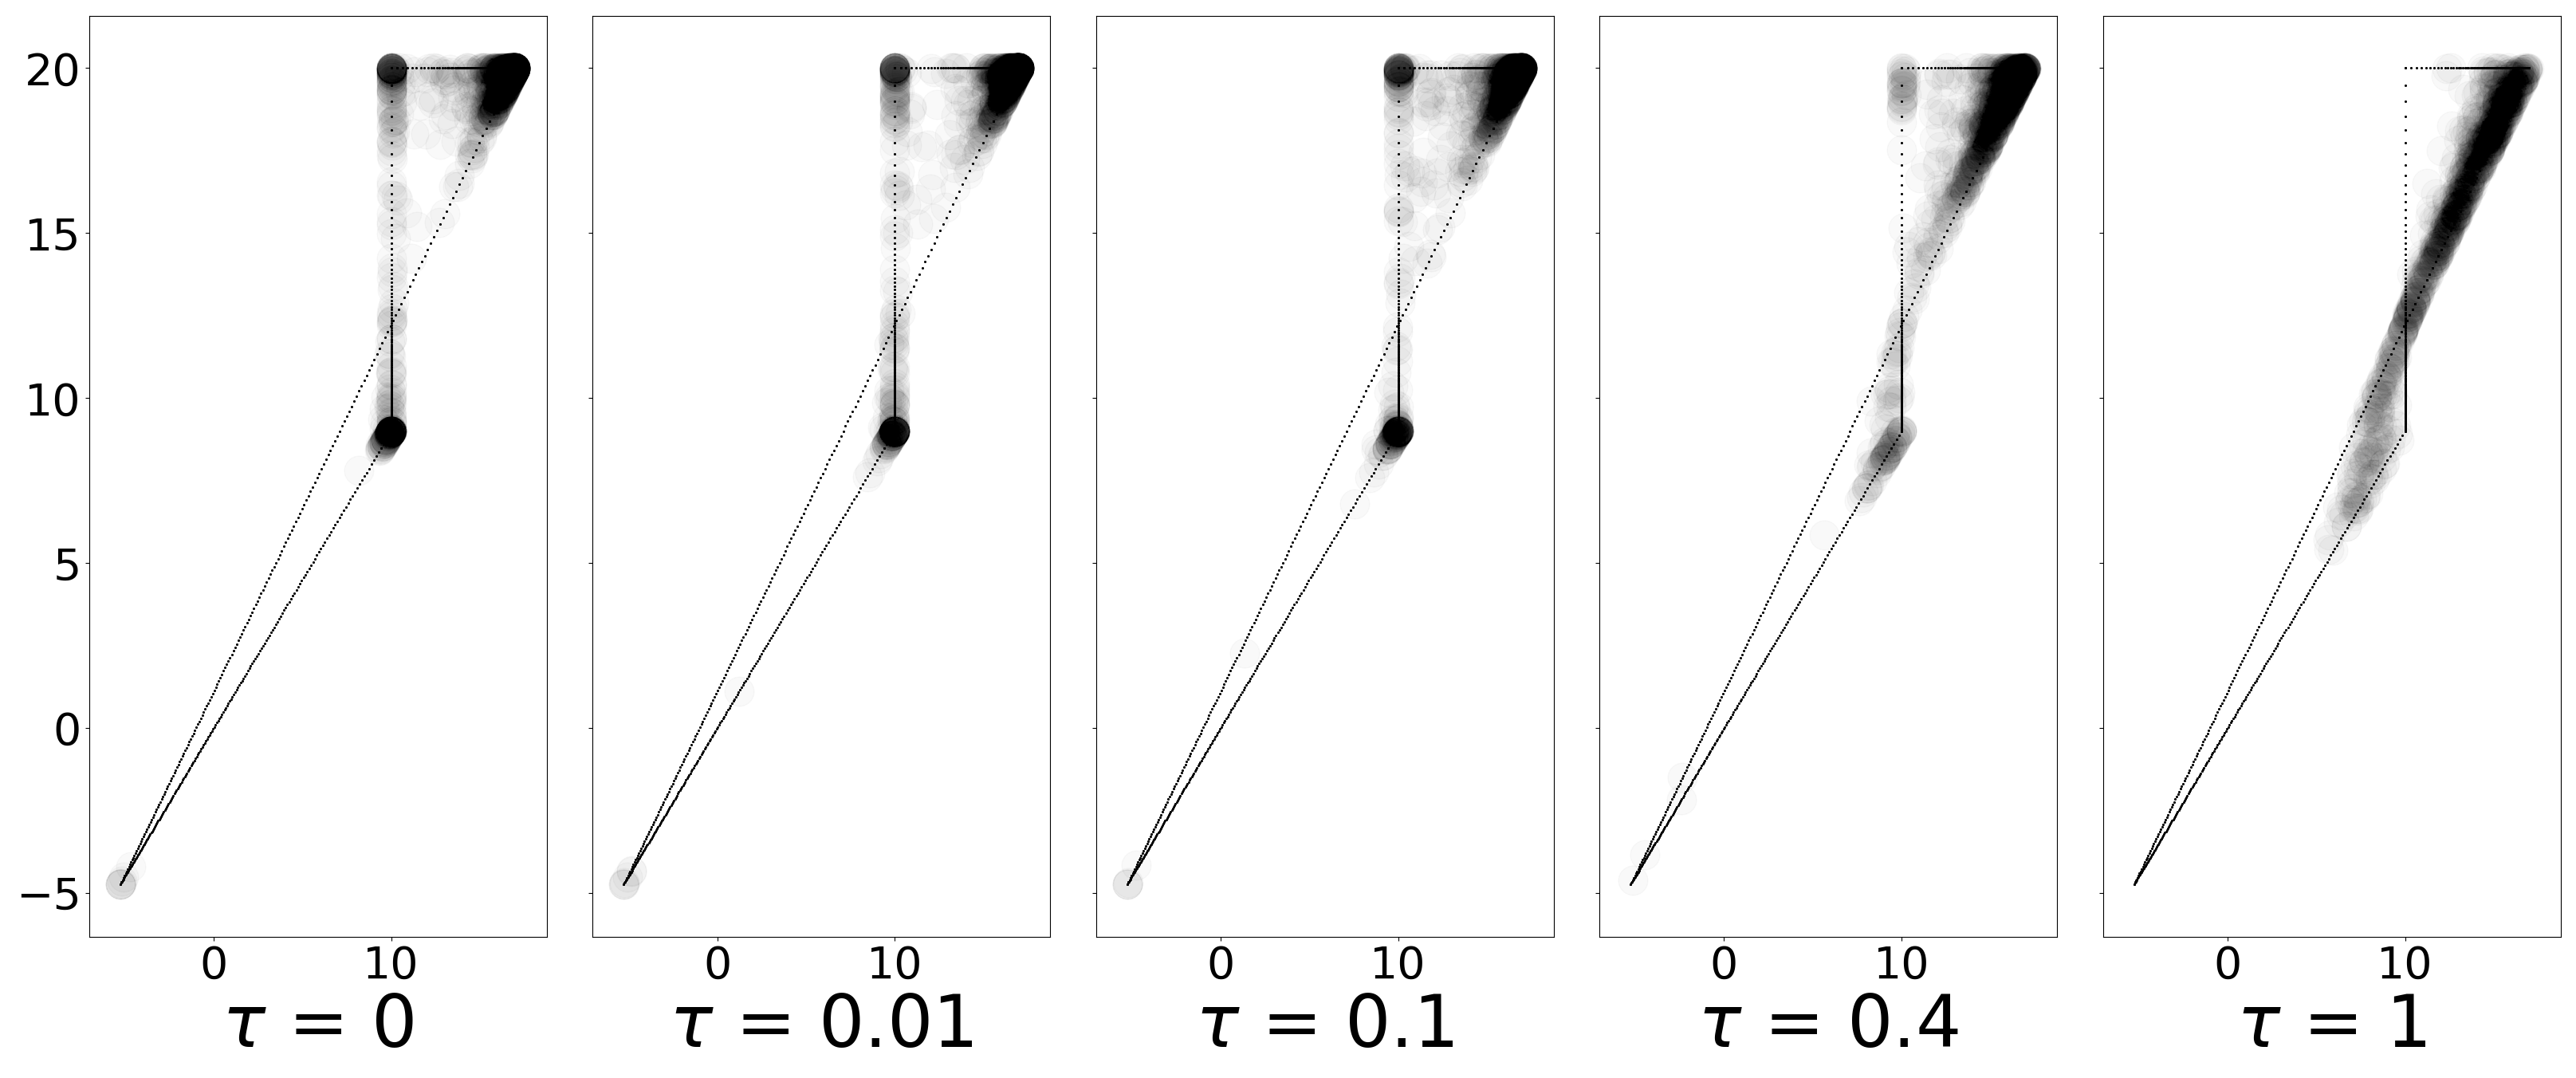
\includegraphics[width=0.8\columnwidth]{figs/continuous-switch-stay/monte-carlo/10/polytope_reverse_optim=rmsprop_lr=0.01.png}
        \caption{Reverse KL.}
        \label{fig:10-sample-switch-stay-reverse}
  \end{subfigure}
  \caption{Switch-stay with 10 sample points, learning rate = 0.01, with RMSprop.}
\end{figure}

% \begin{figure}[!htb]
%   \centering
%   \begin{subfigure}[b]{0.85\linewidth}
%     \centering
%     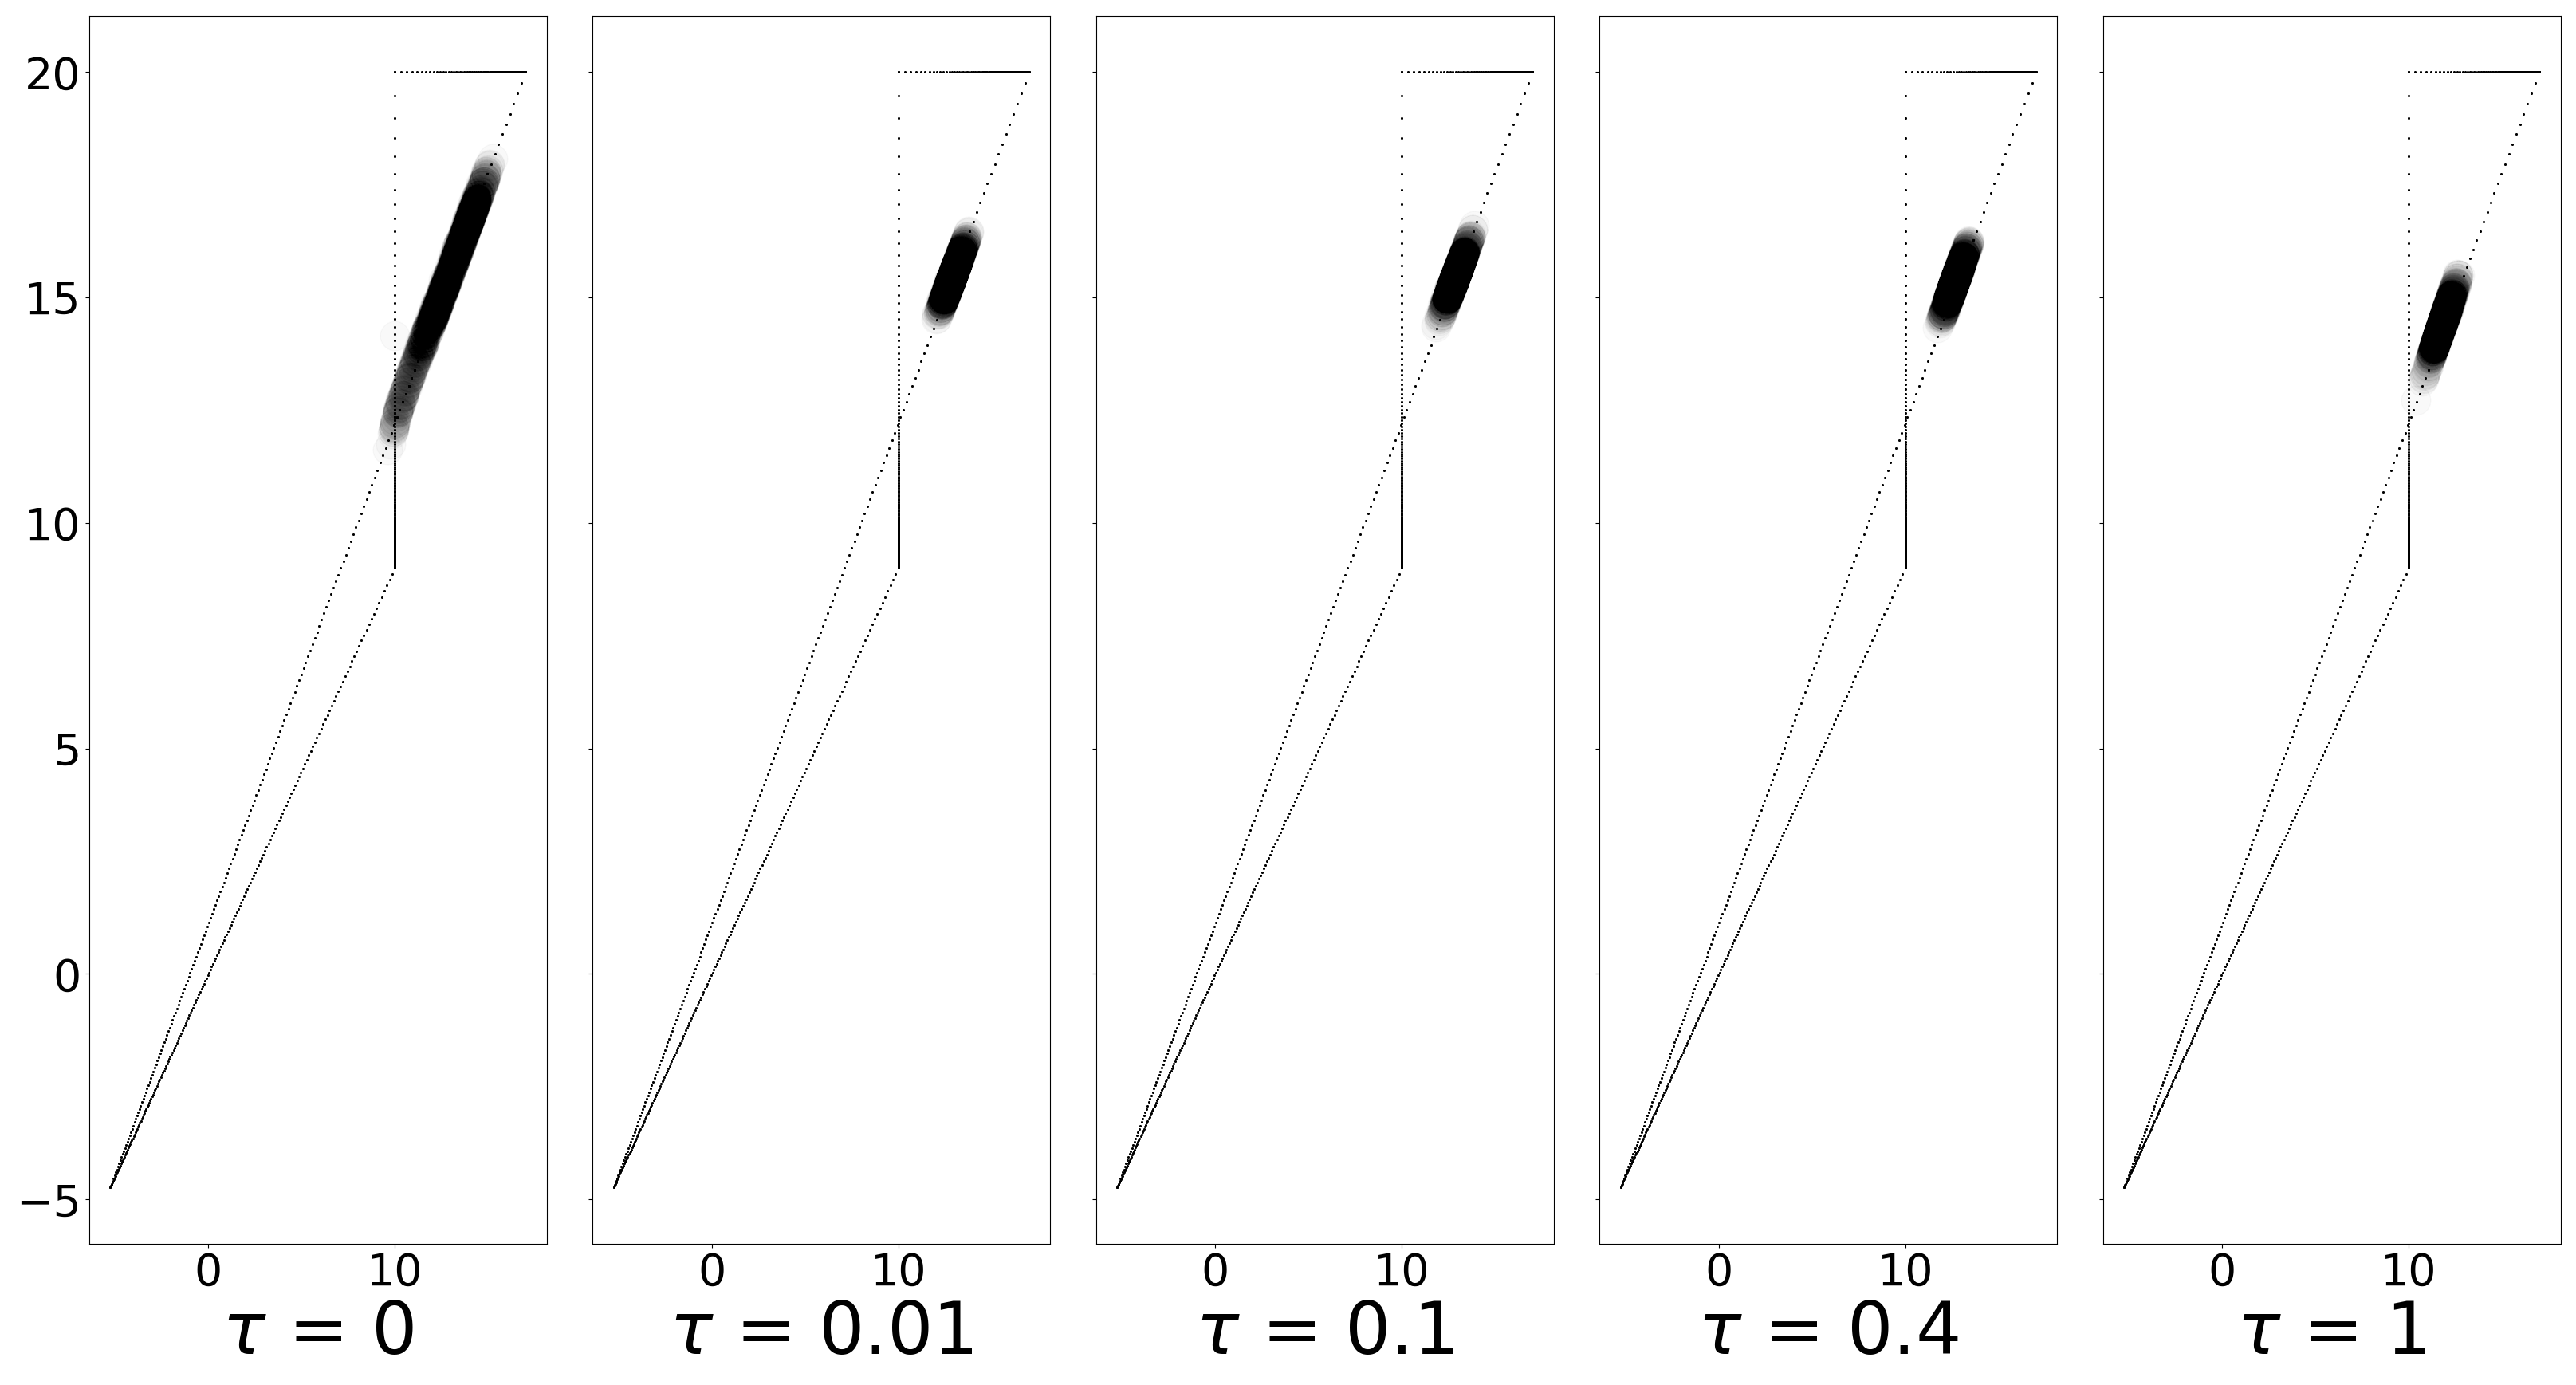
\includegraphics[width=0.8\columnwidth]{figs/continuous-switch-stay/monte-carlo/100/polytope_forward_optim=adam_lr=0.01.png}
%     \caption{Forward KL.}
%     \label{fig:100-sample-switch-stay-forward}
%   \end{subfigure}
  
%   \begin{subfigure}[b]{0.85\linewidth}
%         \centering
%         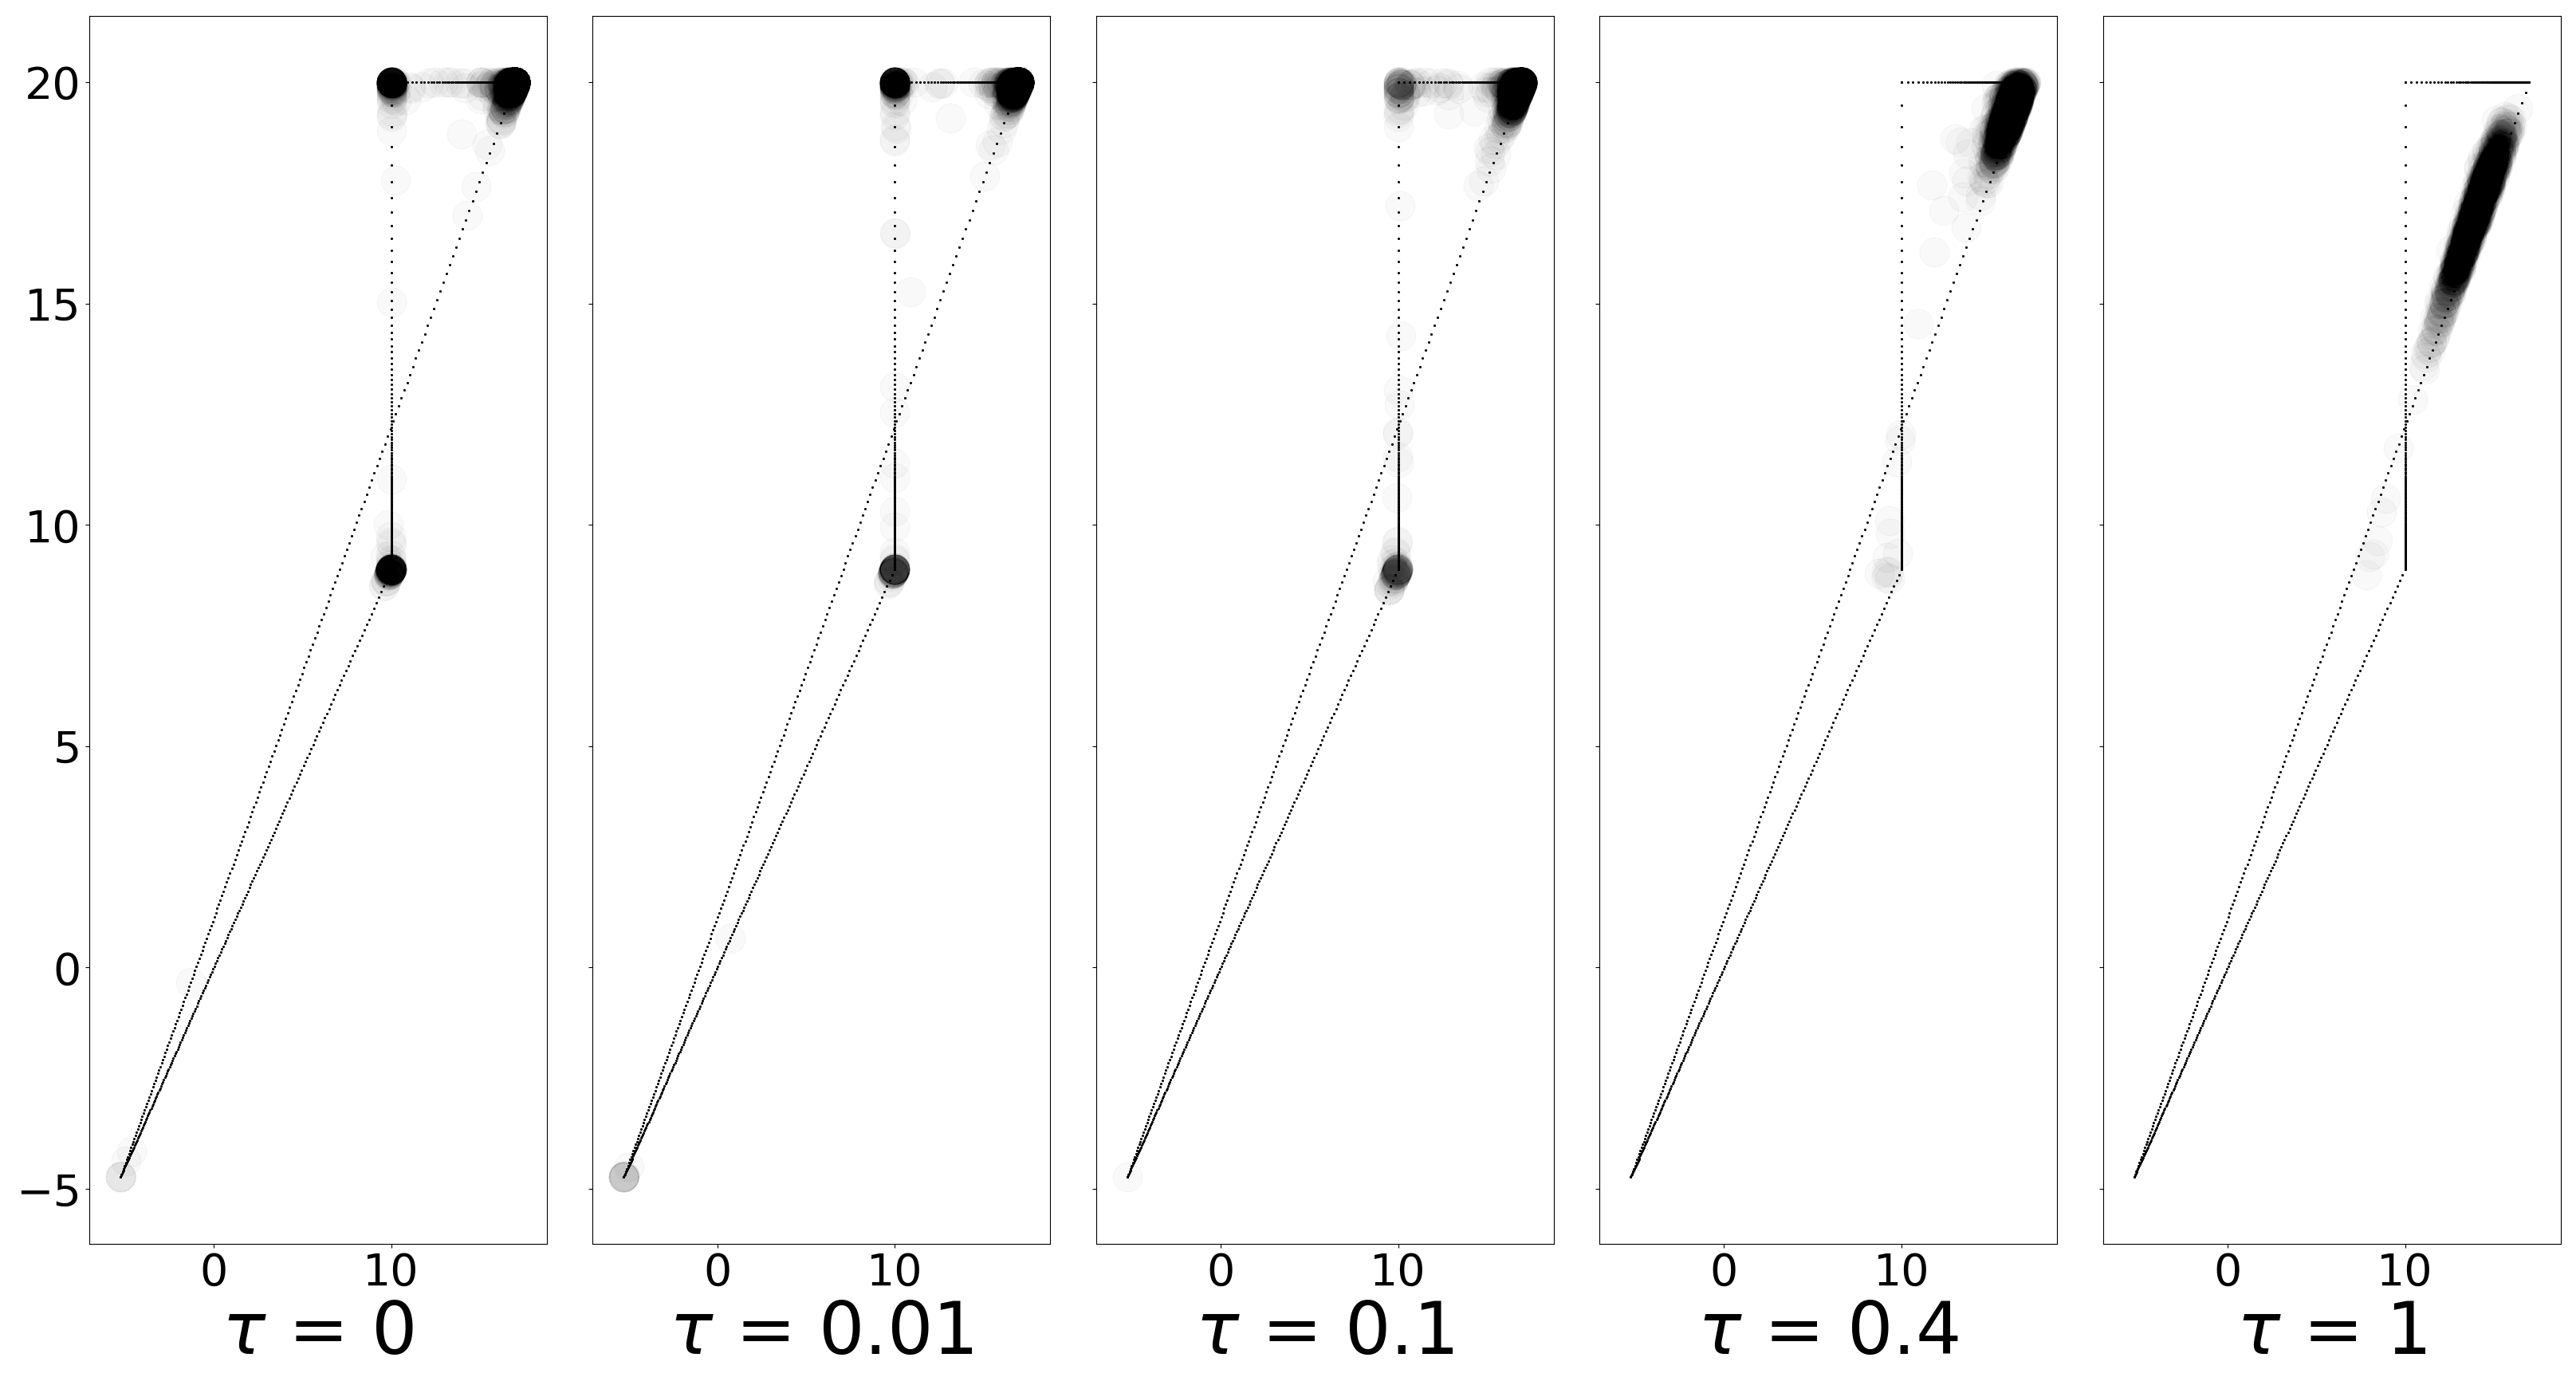
\includegraphics[width=0.8\columnwidth]{figs/continuous-switch-stay/monte-carlo/100/polytope_reverse_optim=adam_lr=0.01.png}
%         \caption{Reverse KL.}
%         \label{fig:100-sample-switch-stay-reverse}
%   \end{subfigure}
%   \caption{Switch-stay with 100 sample points, learning rate = 0.01, with Adam.}
% \end{figure}

% \begin{figure}[!htb]
%   \centering
%   \begin{subfigure}[b]{0.85\linewidth}
%     \centering
%     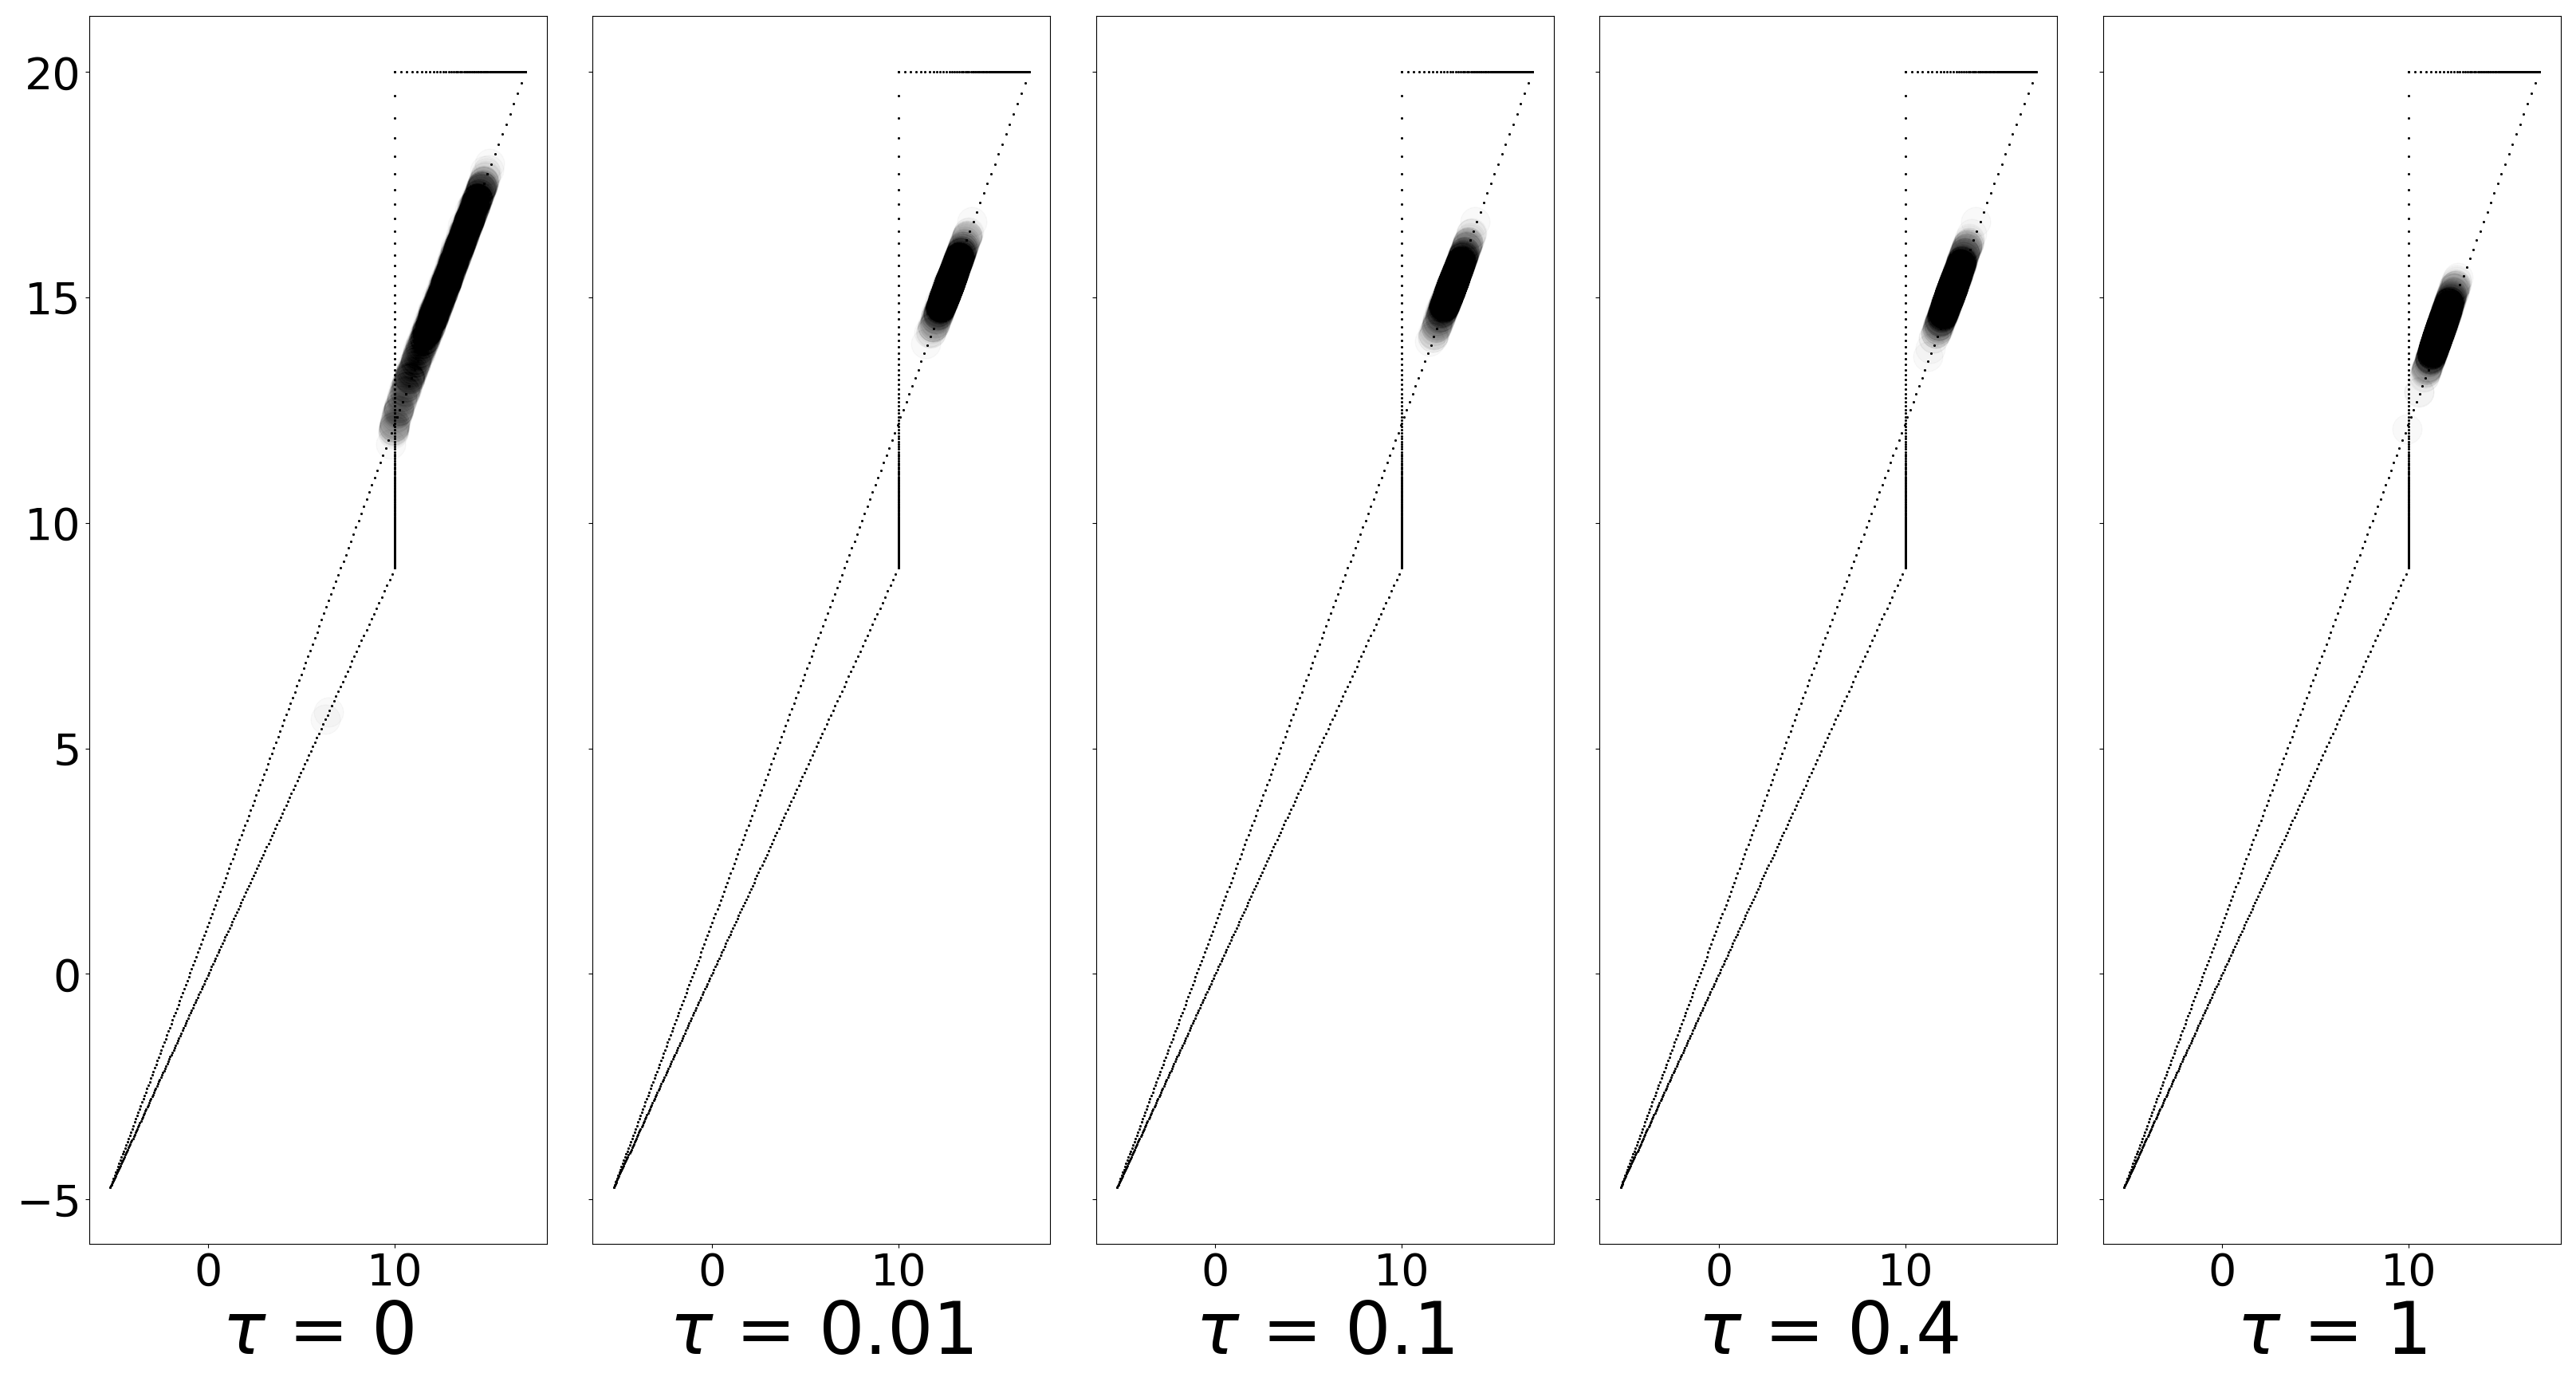
\includegraphics[width=0.8\columnwidth]{figs/continuous-switch-stay/monte-carlo/500/polytope_forward_optim=adam_lr=0.01.png}
%     \caption{Forward KL.}
%     \label{fig:500-sample-switch-stay-forward}
%   \end{subfigure}
  
%   \begin{subfigure}[b]{0.85\linewidth}
%         \centering
%         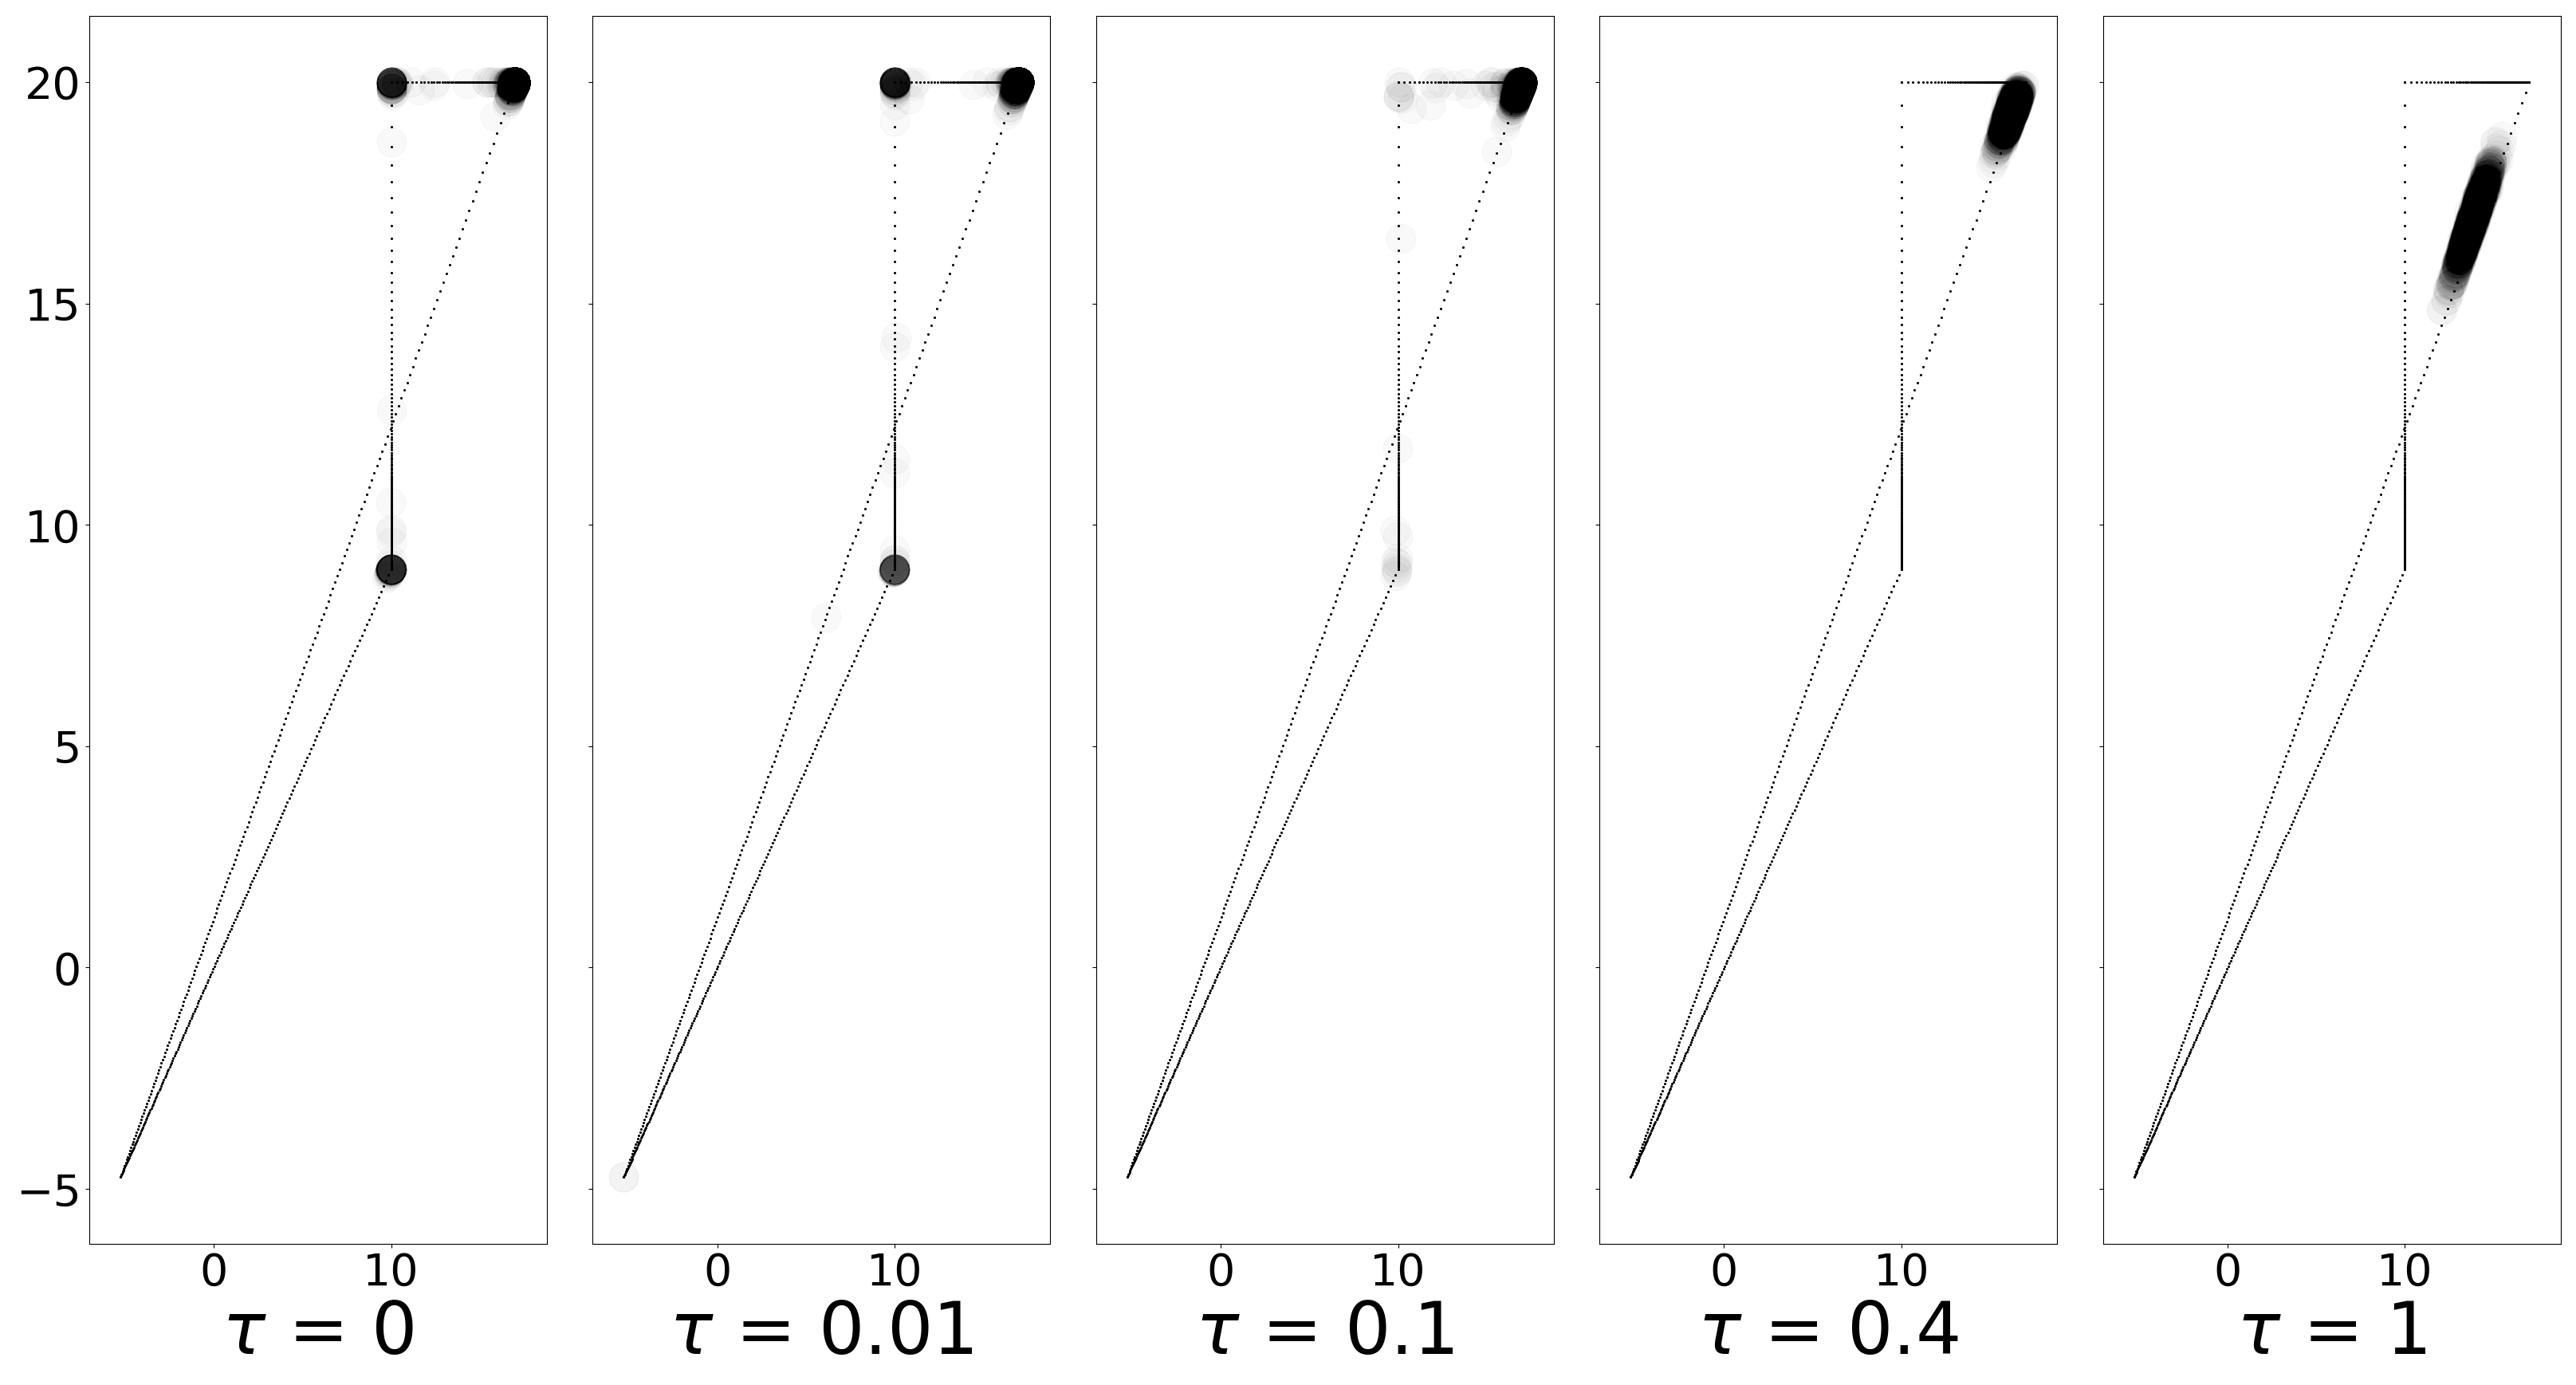
\includegraphics[width=0.8\columnwidth]{figs/continuous-switch-stay/monte-carlo/500/polytope_reverse_optim=adam_lr=0.01.png}
%         \caption{Reverse KL.}
%         \label{fig:500-sample-switch-stay-reverse}
%   \end{subfigure}
%   \caption{Switch-stay with 500 sample points, learning rate = 0.01, with Adam.}
% \end{figure}


\begin{figure}[!htb]
  \centering
  \begin{subfigure}[b]{0.85\linewidth}
    \centering
    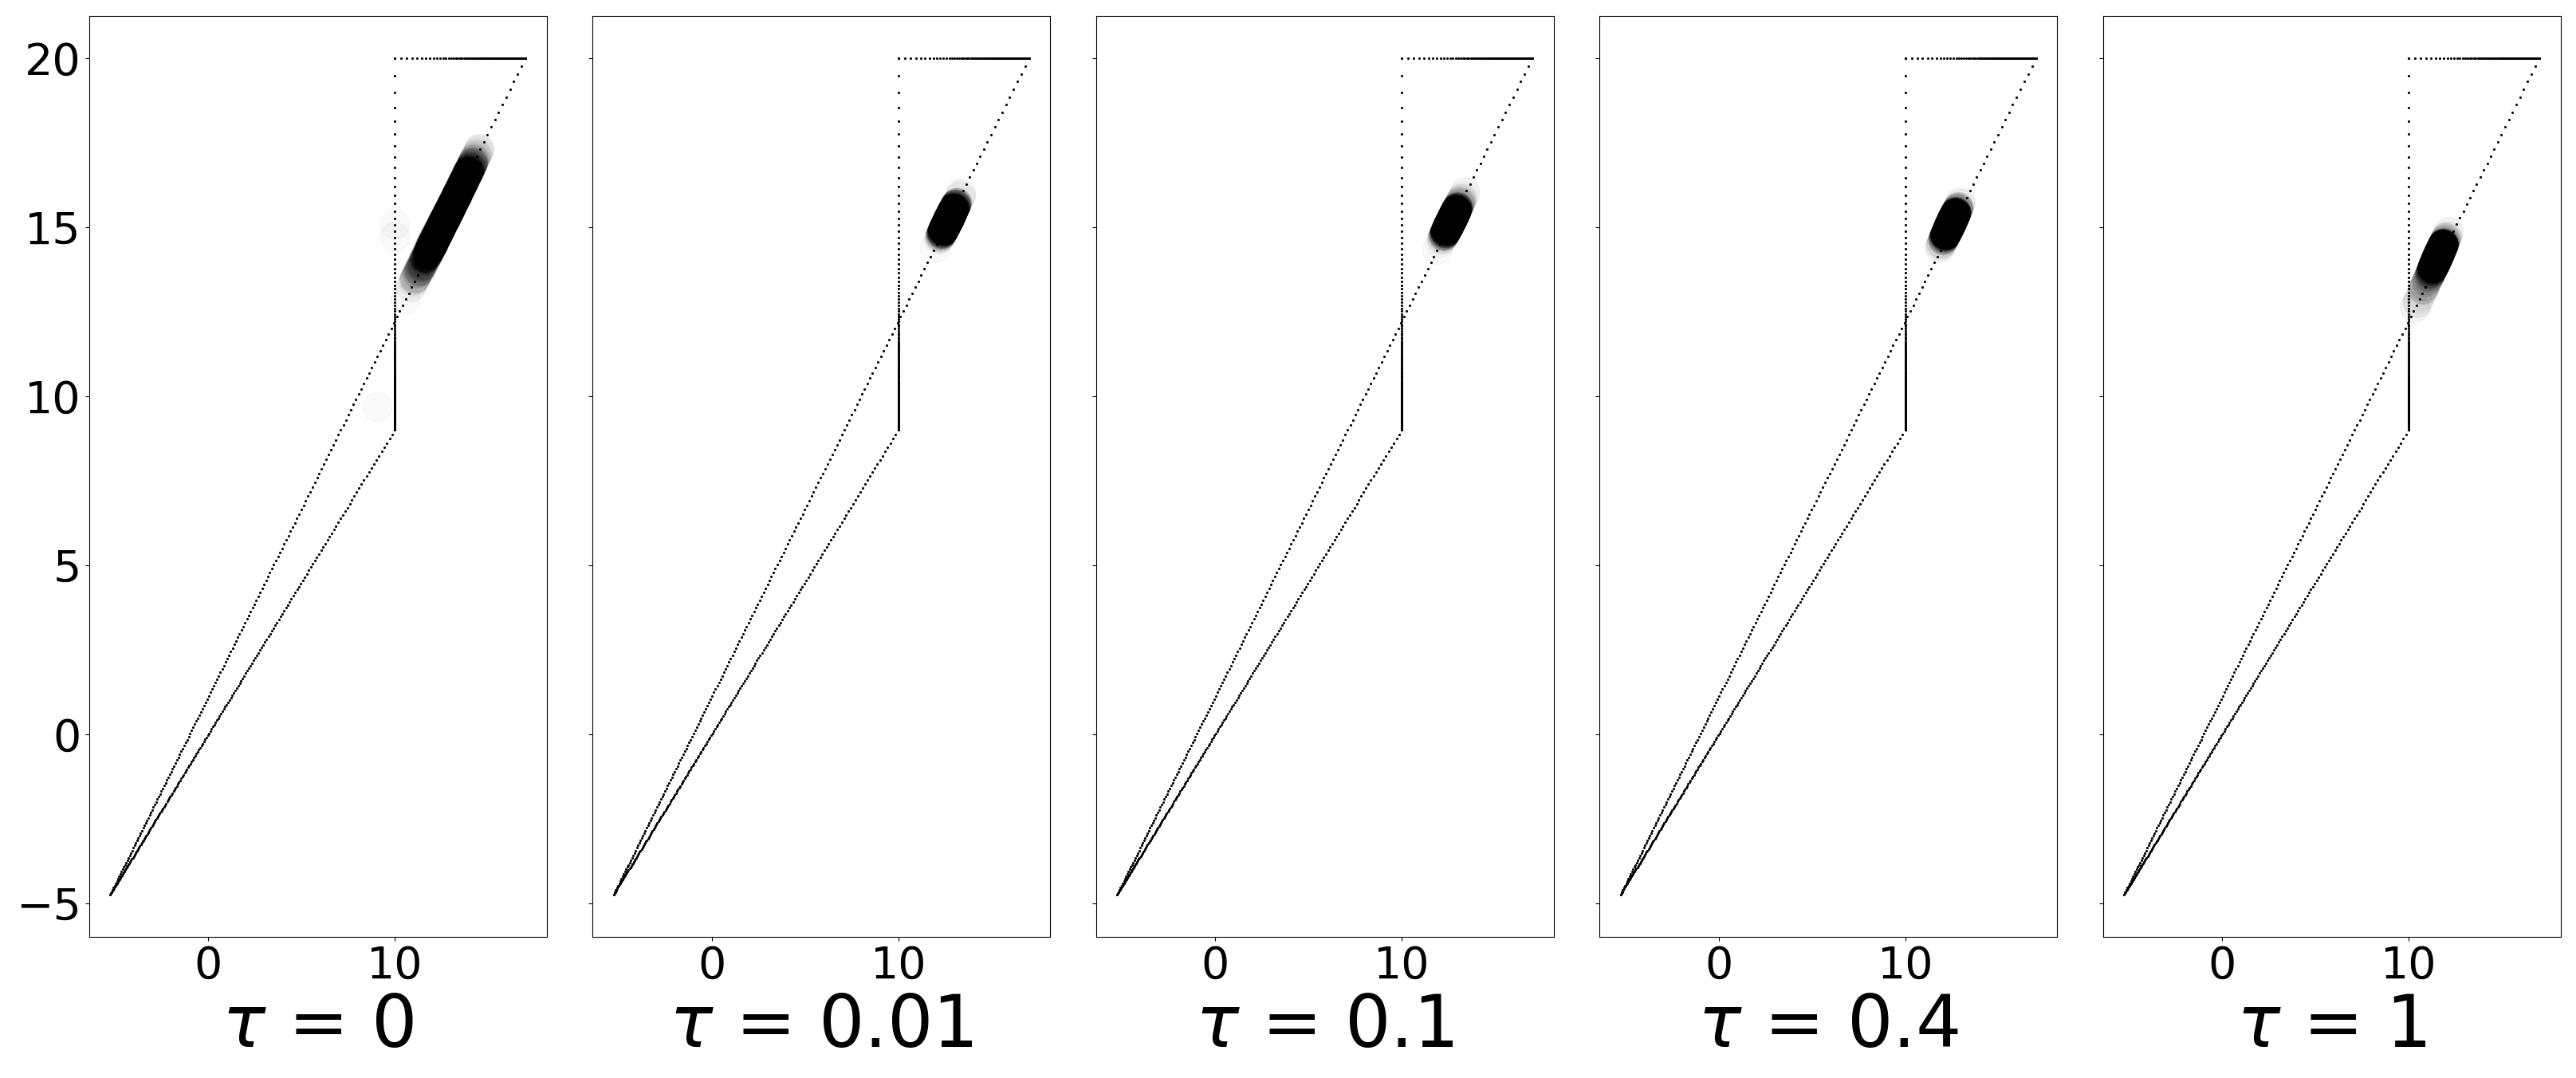
\includegraphics[width=0.8\columnwidth]{figs/continuous-switch-stay/monte-carlo/500/polytope_forward_optim=rmsprop_lr=0.01.png}
    \caption{Forward KL.}
    \label{fig:500-sample-switch-stay-forward}
  \end{subfigure}
  
  \begin{subfigure}[b]{0.85\linewidth}
        \centering
        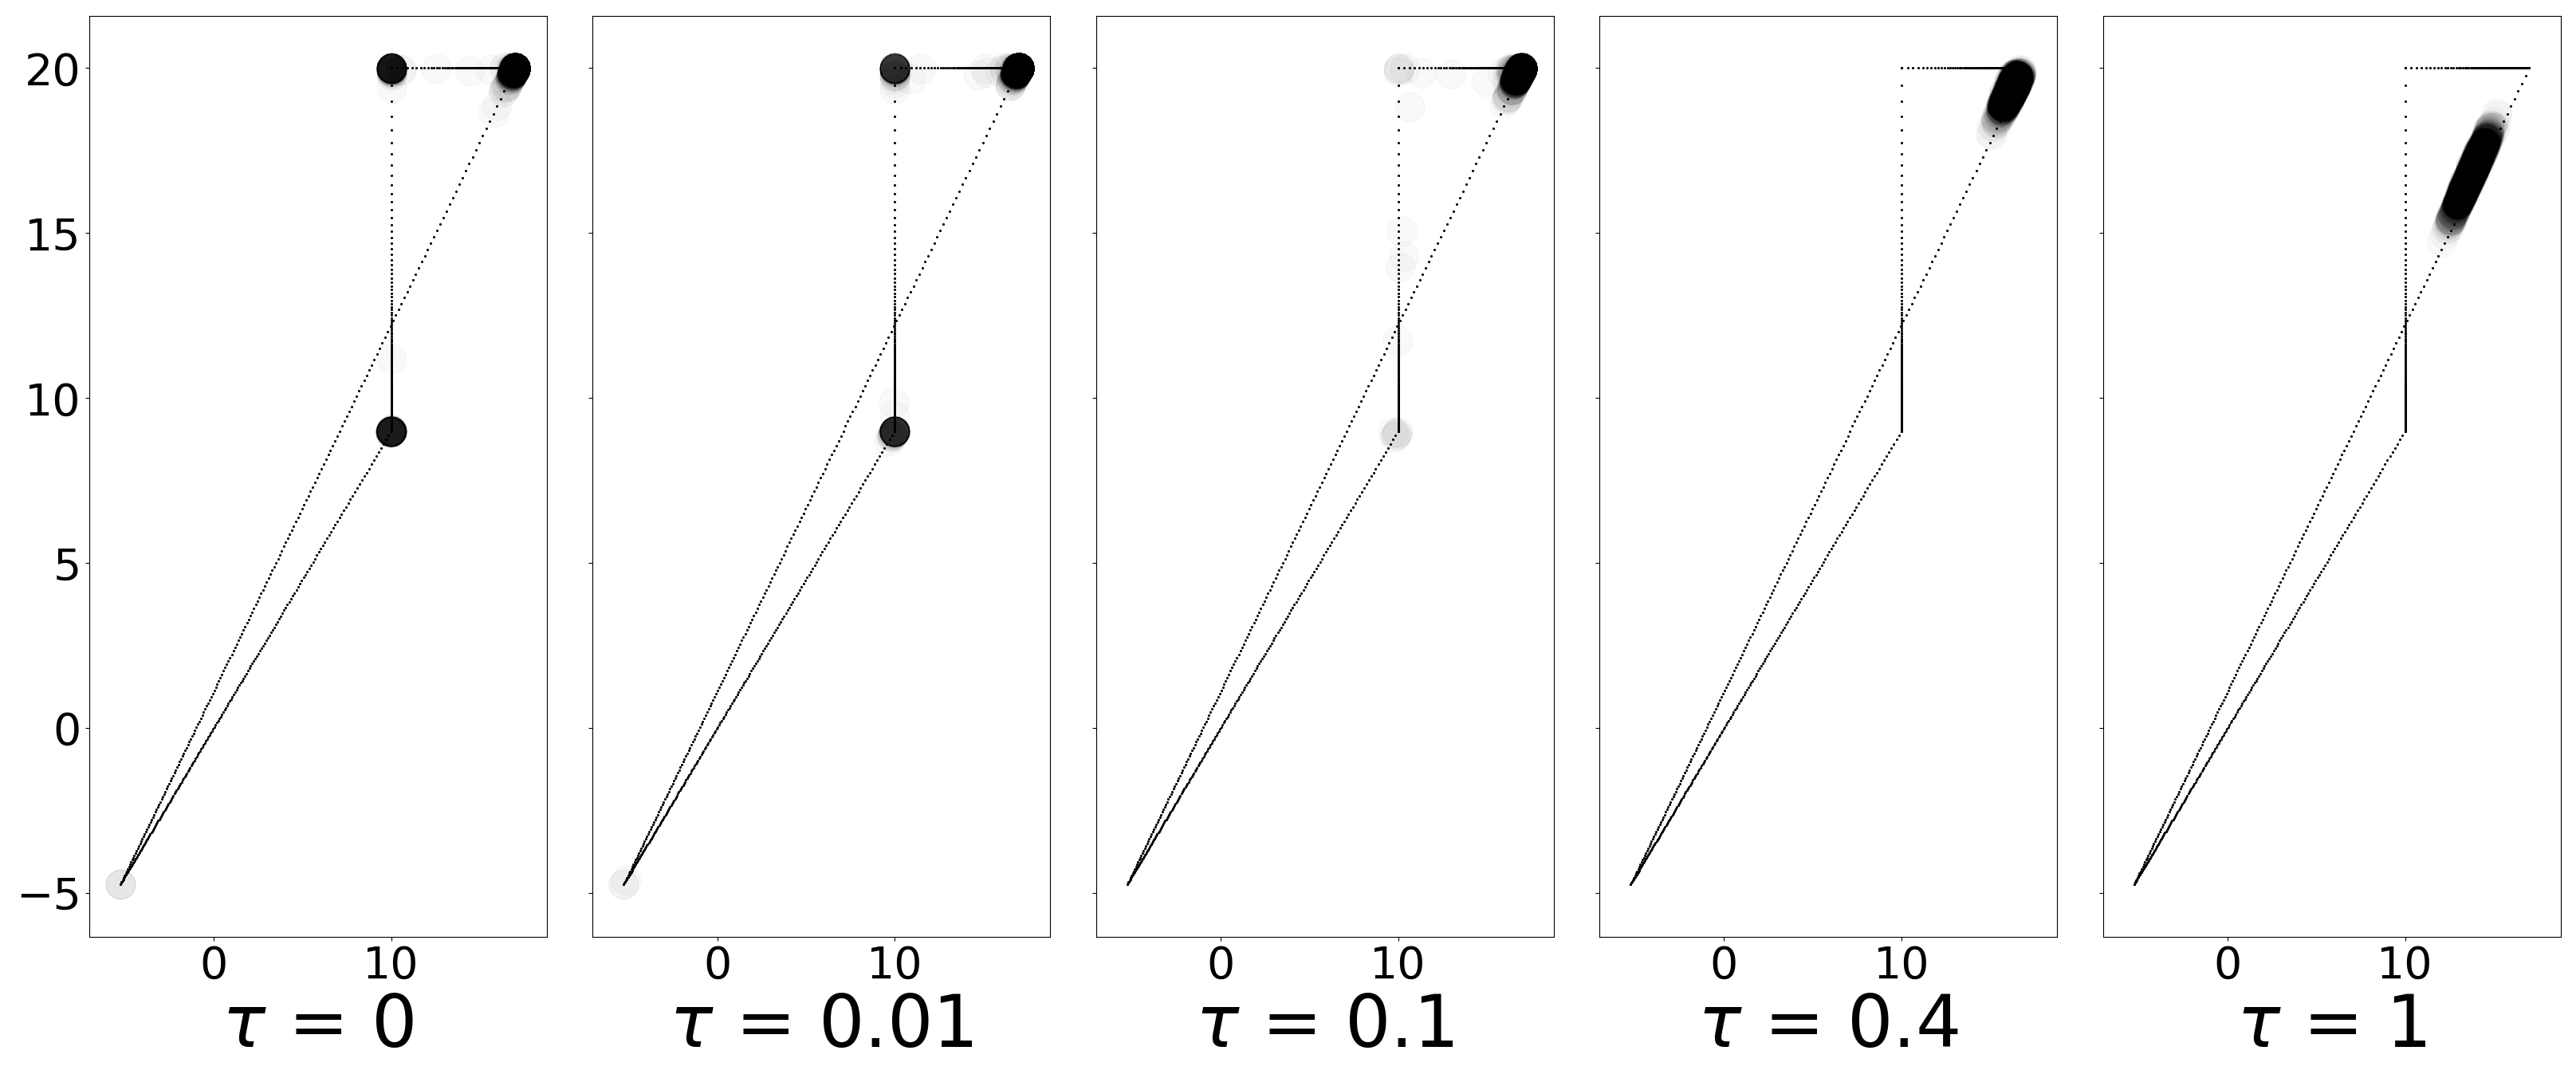
\includegraphics[width=0.8\columnwidth]{figs/continuous-switch-stay/monte-carlo/500/polytope_reverse_optim=rmsprop_lr=0.01.png}
        \caption{Reverse KL.}
        \label{fig:500-sample-switch-stay-reverse}
  \end{subfigure}
  \caption{Switch-stay with 500 sample points, learning rate = 0.01, with RMSprop.}
\end{figure}


On Switch-Stay, more notable differences emerged. RKL iterates converged to minima to which they did not converge in the Clenshaw-Curtis regime, even for larger numbers of sample points. In \Cref{fig:500-sample-switch-stay-reverse}, there is an interesting trend across temperatures. Temperatures below $0.4$ induced many suboptima far from the optimal value function, while temperatures 0.4 and 1 seemed better at clustering RKL iterates near the optimal value function. On the other hand, FKL seemed relatively insensitive both to the temperature and the number of sample points. This relative insensitivity could be due to having a smoother loss landscape to begin with, which tends to direct iterates to a single global optimum. Nevertheless, that global optimum was often quite suboptimal with respect to the unregularized MDP, especially since many RKL iterates were much closer to the optimal policy of the unregularized MDP. 


\subsection{Summary}
Given the amount of data in this chapter, it is helpful to summarize our discussion thus far. 
\begin{enumerate}
    \item The relative difference between the KLs in continuous-action settings is larger than that in discrete-action settings. 
    \item On our bimodal bandit, the FKL was better at directing iterates to the global optimum, excepting some iterates that stayed near the suboptimal mode when the initial standard deviation was set sufficiently low. However, as the temperature increased, the global optimum of the FKL seemed to approach a suboptimal point with respect to the bandit reward function faster than the global optimum of the RKL did. 
    \item On the continuous version of Switch-Stay, the FKL iterates converged more slowly than the RKL iterates and to a policy that was less optimal, which seemed primarily due to a larger final standard deviation for the FKL iterates. The increased suboptimality of the FKL solution is consistent with our bandit results. 
    \item In the continuous-action setting, stochastic sampling of the loss function impacted RKL more than FKL. RKL tended to exhibit more spurious minima in this setting, even when increasing the number of sample points in the calculation of the loss. 
    \item In the discrete-action setting, little significant difference emerged between FKL and RKL. Both converged to nearly identical optima, although the convergence of iterates under FKL seemed slightly slower. 
\end{enumerate}

We suspect that the differences here are heavily due to the policy parameterization. One reason for the difference in the number of minima seems to be that a Gaussian policy is unimodal, whereas a softmax policy can represent multimodal distributions. As well, given that the behaviour in the bandit setting depended on the initial standard deviation, we hypothesize that the added complexity of learning the standard deviation contributes to the differences we observed between continuous and discrete actions. 


We also did not learn action-values in our experiments. Especially given the additional differences between the KLs that we observed with stochasticity, using learned action-values might drastically change our results. In this setting, the accuracy of the action-value estimate would depend on the actions taken by the agent, which in turn are affected by the process of policy optimization. For instance, if an agent tends to commit to an action at a given state and not try other actions, the resulting action-value estimate could be poor. In the literature in general, more investigation into the interplay of learning value functions and policy optimization is necessary. 

%------------------------------------------------------------------------------------------------------------------------------
\subsection{Practical Performance on Benchmark Problems}

We compare the KL methods on benchmark continuous and discrete-action environments, using non-linear function approximation. Here, we wish to understand (1) if our observations from the microworld experiments apply to more complicated environments and (2) if any new differences as a result of function approximation or increased environment complexity. 

\subsection{Implementation Details}
\subsubsection{Hyperparameters}
Hyperparameter sweeps are performed separately for each domain. We sweep over the learning rates $\{10^{-5}, 10^{-4}, 10^{-3}\}$; for Pendulum, we additionally sweep over actor learning rate $10^{-2}$. In the continuous-action setting, we sweep both the actor and the critic learning rate, while in the discrete-action setting we have a shared learning rate because of a shared architecture. We sweep temperatures in $\{0.01, 0.1, 1\}$ for the soft action-value methods and set the temperature in $\boltzmannQ$ and the temperature in the soft action-value function to be the same value. For example, if $\tau = 0.01$, then we learn a soft action-value function with $\tau = 0.01$ and use a KL target distribution proportional to $\exp(Q(s, a) \tau^{-1})$. RMSprop \citep{tieleman2012lecture} is used as the optimizer to be consistent with our focus in the microworld domains. 

We perform 30 runs for all hyperparameter settings and plot the mean return averaged over the past 20 episodes; shaded areas represent standard errors. 


\subsubsection{Updating}
We perform bootstrapping as per the recommendations in \citet{pardo2017time}. If a transition $(s, a, r, sp)$ results in the true termination of the episode, the bootstrap target for value function updates is $r$ instead of the usual $r - \tau \log \pi(a \mid s) + \gamma V(sp)$. If the transition results in a timeout, $r - \tau \log \pi(a \mid s) + \gamma V(sp)$ is used. Otherwise, $r - \tau \log \pi(a \mid s) + \gamma V(sp)$ is used as the bootstrap target. 

On the continuous-action domains we use Clenshaw-Curtis \citep{clenshaw1960method} numerical integration scheme to estimate the FKL and the RKL. To generate the points for Clenshaw-Curtis, we use the Python package, quadpy.\footnote{\url{https://github.com/nschloe/quadpy}}. For computational efficiency, we use 64 points for 1D environments, and $l=6$ for multi-dimensional environments using the nested univariate quadrature formula for Clenshaw-Curtis \citep{gerstner1998numerical}. In learning value functions we learn both $Q(s, a)$ and $V(s)$, using the same target as done in SAC \citep{haarnoja2018soft}. In particular, the target for $V(s)$ is $Q(s, a) - \log(\pi(a \mid s))$. On preliminary experiments, we found that the target of $Q(s, a) - \log(\pi(a \mid s))$ performed better than the target of $r(s) - \tau \log \pi(a \mid s) + \gamma V(s')$ for all methods.

On the discrete-action domains, the value function update target is $r(s) - \tau \log \pi(a \mid s) + \gamma V(s')$ instead of the update that SAC uses, $Q(s, a) - \log \pi(a \mid s)$. Preliminary experiments indicated that the former update was superior for all methods. Both $Q$ and $V$ are learned. 

For reference, we also include the gradient updates of the various KL divergences. 
\begin{align}
    &\textbf{RKL}: \nabla_\theta \KL(\pi_\theta(\cdot \mid s) \parallel \boltzmannQ_\tau(s, \cdot)) \nonumber\\
    &\quad= -\nabla_\theta \entropy(\pi_\theta(\cdot \mid s)) - \int_\actionspace\nabla_\theta \pi_\theta(a \mid s) \log \boltzmannQ_\tau(a \mid s)\, da \label{eq:rkl-gradient}\\
    &\textbf{FKL}: \nabla_\theta \KL(\boltzmannQ_\tau(s, \cdot) \parallel \pi_\theta(\cdot \mid s) )\nonumber\\
    &\quad= - \int_\actionspace  \boltzmannQ_\tau(a \mid s) \nabla_\theta \log \pi_\theta(a \mid s) \, da \label{eq:fkl-gradient} \\
    &\textbf{Hard RKL}: - \int_\actionspace\nabla_\theta \pi_\theta(a \mid s) Q(s, a)\, da \label{eq:hrkl-gradient}\\
    &\textbf{Hard FKL}: -\nabla_\theta \log \pi_\theta \left(\argmax_b Q(s, b) \mid s\right) \label{eq:hfkl-gradient}.
\end{align}

\begin{algorithm}
\caption{Agent for Benchmark Experiments}
\label{alg:kl-agent}
\begin{algorithmic}
    \State Given: policy $\pi_\theta$ (parameters $\theta$); action-value estimate $Q_v$ (parameters $v$); state-value estimate $V_w$ (parameters $w$); experience replay buffer; choice of KL divergence; temperature $\tau \geq 0$; learning rates for $\theta$, $v$, $w$; optimizer (e.g., RMSprop).
    \For{$t = 0, \ldots,$}
        \State Draw action $a_t \sim \pi_\theta(\cdot \mid s_t)$
        \State Observe and store transition $(s_t, a_t, s_{t + 1}, r, \text{DoneFlag})$. Replace the oldest transition if the buffer size limit is reached. 
        \If{samples in buffer $\geq$ 32}
            \State Draw random mini-batch of size 32 from buffer. 
            \For{each transition $(s, a, r, sp, \text{DoneFlag})$ in the mini-batch}
                \State Calculate KL gradients according to \Cref{eq:rkl-gradient,eq:fkl-gradient,eq:hrkl-gradient,eq:hfkl-gradient}, based on choice of $\tau$ and KL divergence.
            \EndFor
            \State Update $w, v$ with DiscreteUpdateValueFunctions if action space is discrete; otherwise call ContinuousUpdateValueFunctions.
            \State Update $\theta$ with the learning rate and optimizer.
        \EndIf
    \EndFor
\end{algorithmic}
\end{algorithm}

\begin{algorithm}
\caption{DiscreteUpdateValueFunctions}
\label{alg:discrete-value-update}
\begin{algorithmic}
    \State Given: policy $\pi_\theta$ (parameters $\theta$); action-value estimate $Q_v$ (parameters $v$); state-value estimate $V_w$ (parameters $w$); temperature $\tau \geq 0$;  optimizers (e.g., RMSprop) for $v$ and $w$; batch of data $\mathcal{D}$, with each transition written in the form $(s, a, r, sp, \text{DoneFlag})$
    \State To update the state-value function, pass the following as the gradient to the optimizer for $w$. 
    \begin{align*}
        -\Ex_{\mathcal{D}}[(r - \tau \log \pi(a \mid s) + \gamma\cdot (1 - \text{DoneFlag})\cdot V_w(sp) - V(s)) \nabla_w V(s)]
    \end{align*}
    \State To update the action-value function, pass the following as the gradient to the optimizer for $v$. 
    \begin{align*}
        -\Ex_{\mathcal{D}}[(r + \gamma \cdot (1 - \text{DoneFlag})\cdot V_w(sp) - Q_v(s, a)) \nabla_v Q_v(s, a)]
    \end{align*}
\end{algorithmic}
\end{algorithm}

\begin{algorithm}
\caption{ContinuousUpdateValueFunctions}
\label{alg:continuous-value-update}
\begin{algorithmic}
    \State Given: policy $\pi_\theta$ (parameters $\theta$); action-value estimate $Q_v$ (parameters $v$); state-value estimate $V_w$ (parameters $w$); temperature $\tau \geq 0$; optimizers (e.g., RMSprop) for $v$ and $w$; batch of data $\mathcal{D}$, with each transition written in the form $(s, a, r, sp, \text{DoneFlag})$
    \State For each state $s$ in the batch $\mathcal{D}$, draw a new action $\tilde{a} \sim \pi_\theta(\cdot \mid s)$.
    \State To update the state-value function, pass the following as the gradient to the optimizer for $w$. 
    \begin{align*}
        \Ex_{\mathcal{D}}[(V_w(s) - Q_v(s, \tilde{a}) + \tau \log \pi_\theta (\tilde{a} \mid s)) \nabla V_w(s)]
    \end{align*}
    \State To update the action-value function, pass the following as the gradient to the optimizer for $v$. 
    \begin{align*}
        -\Ex_{\mathcal{D}}[(r + \gamma \cdot (1 - \text{DoneFlag})\cdot V_w(sp) - Q_v(s, a)) \nabla_v Q_v(s, a)]
    \end{align*}
\end{algorithmic}
\end{algorithm}

In all our plots, we refer to the number of ``frames'' on the $x$-axis. We use ``frames'' synonomously with ``timestep''. 

\subsubsection{Architecture}
On our continuous-action domains, all policy and value function networks are implemented as two-layer neural networks of size 128, with ReLU activations. We use experience replay of buffer size $10^6$ with batch size of 32. On our discrete-action domains, we employ the following architectures.

\textbf{OpenAI Gym}: The architecture is a two-layer neural network, with the policy and value functions as separate heads off of the main two-layer body. ReLU activations are used between layers. We report results for three hidden layer sizes: small (32), medium (128), and large (512).

\textbf{MinAtar}: The architecture is a convolutional network into one fully-connected layer for each of the policy, action value function, and state value function. The convolutional layer has 16 3x3 convolutions with stride 1, the same as in \citet{young2019minatar}; we vary the size of the fully-connected layer in $\{32, 128\}$. ReLU activations are used between layers. 

On the discrete-action domains, experience replay is used with a buffer size of $10^5$ and a batch size of 32. 

\subsection{Continuous-Action Results}
We compare agents on Pendulum \citep{brockman2016openai}, Reacher, and Swimmer \citep{todorov2012mujoco}, with results shown in Figure \ref{fig_cont}. We exclude Hard FKL in our comparison since it requires access to $\max_a Q(s,a)$, which is difficult to obtain with continuous actions. 


\begin{figure}[t]
  \centering
  \begin{subfigure}[b]{0.5\linewidth}
    \centering
    \includegraphics[width=\columnwidth]{figs/deep/continuous/PD_entropy_comparison.pdf} 
    \caption{Pendulum}\label{fig:pendulum}
  \end{subfigure}%
  \begin{subfigure}[b]{0.5\linewidth}
    \centering
    \includegraphics[width=\columnwidth]{figs/deep/continuous/Reacher_entropy_comparison.pdf} 
    \caption{Reacher}\label{fig:reacher}
  \end{subfigure}
  
  \begin{subfigure}[b]{0.5\linewidth}
    \centering
    \includegraphics[width=\columnwidth]{figs/deep/continuous/Swimmer_entropy_comparison.pdf} 
    \caption{Swimmer}\label{fig:swimmer}
  \end{subfigure}
  \caption{Continuous-action environments. Shown are the best hyperparameters for each algorithm, which are selected by largest area under the last half of the learning curve. The colours go from hot (red, temperature = 1) to cool (yellow, temperature = 0). }\label{fig_cont}
\end{figure}

For certain temperatures, FKL either learns faster than or achieves superior final return to RKL. This difference is especially striking on Pendulum \Cref{fig:pendulum}, where FKL learns vastly faster than RKL for $\tau = 0.1, 0.01$. It's interesting to note that RKL with $\tau = 1$ has a similarly-shaped learning curve to FKL with $\tau = 0.01, 0.1, 1$. In a sense, the higher temperature of RKL with $\tau = 1$ might be compensating for committal behaviour of RKL that we observed in the microworld experiments. It does seem possible to be too non-committal. On Reacher in \Cref{fig:reacher}, FKL with $\tau = 1$ completely fails to learn, while all other settings learn appreciably. Nevertheless, these observations suggest a connection between the impacts of FKL and of entropy regularization, as we discuss further below in the discrete-action setting. 

It is difficult to comment on the importance of the policy parameterization for these experiments relative to our microworld experiments. Any influence from the Gaussian policy parameterization is conflated with function approximation. Moreover, as we will see below, no stark pattern seems to divide continuous and discrete action settings, as one did in our microworld experiments. 

\section{Discrete-Action Results}
We report results for environments from the OpenAI gym \citep{brockman2016openai} and MinAtar \citep{young2019minatar}. 



\begin{figure}[t]
  \centering
  \begin{subfigure}[b]{1\linewidth}
    \centering
    \includegraphics[width=\columnwidth]{figs/deep/discrete/acrobot_combined.png} 
    \caption{Acrobot}\label{fig:acrobot}
  \end{subfigure}%
  
  \begin{subfigure}[b]{1\linewidth}
    \centering
    \includegraphics[width=\columnwidth]{figs/deep/discrete/cartpole_combined.png}
    \caption{CartPole}\label{fig:cartpole}
  \end{subfigure}
  
  \begin{subfigure}[b]{1\linewidth}
    \centering
    \includegraphics[width=\columnwidth]{figs/deep/discrete/lunar_combined.png}
    \caption{Lunar Lander.}
    \label{fig:lunar-lander}
  \end{subfigure}
  \caption{OpenAI Gym discrete-action environments. Plot settings are identical to Figure \ref{fig_cont}.}\label{fig:open-ai}
\end{figure}

% In Acrobot, FKL dominates RKL for all temperatures except $\tau = 1$, which did not learn at all.  This last trend could be because RKL ``commits'' more to actions with high density (i.e., have lower standard deviation, all other things being equal), which we observed in the microworld experiments as well. In CartPole, FKL at $\tau = 0.01, 0.1$ seems to learn a little bit faster than CartPole for hidden layer size $= 128, 256$. In Lunar Lander, FKL with non-zero temperature consistently matches or exceeds the corresponding learning curve for RKL. Indeed, when $\tau = 0$, a large gap separates FKL and RKL. A possible reason  

The results on the OpenAI Gym environments suggest that for small hidden layer sizes, FKL may be at least as good as RKL, and sometimes better. As the hidden layer size increases, however, this dominance is negated. For a hidden layer size of 128, RKL seems to learn a little bit faster than FKL for $\tau \neq 1$, and RKL has a slightly higher final performance for a hidden layer size of 512, although the difference does not appear to be significant. It is possible that these observations are related to how the optimization landscape of a neural network changes with larger hidden layer sizes. The influence of the choice of policy gradient objective on the optimal function approximation architecture deserves further consideration. 

The superiority of FKL in Lunar Lander for $\tau = 0, 0.01$ and sometimes $\tau = 0.1$ is interesting. For these temperatures, FKL with non-zero temperature consistently matches or exceeds the corresponding learning curve for RKL. Indeed, when $\tau = 0$, a large gap separates FKL and RKL. A possible reason for this dominance is the difficulty of exploration in Lunar Lander: one must learn to manoeuvre the spacecraft, discover the correct landing area, learn how to land correctly, and learn to turn off the fuel. That FKL might ``commit'' less (i.e., have higher standard deviation than RKL, all other things equal) suggests that more actions are tried to facilitate discovery of good actions. We further discuss exploration below in our MinAtar experiments. 

\begin{figure}[!htb]
  \centering
  \begin{subfigure}[b]{1\linewidth}
    \centering
    \includegraphics[width=\columnwidth]{figs/deep/discrete/asterix_combined.png} 
    \caption{Asterix
    }\label{fig:asterix}
  \end{subfigure}%
  
  \begin{subfigure}[b]{1\linewidth}
    \centering
    \includegraphics[width=\columnwidth]{figs/deep/discrete/breakout_combined.png} 
    \caption{Breakout
    }\label{fig:breakout}
  \end{subfigure}%
  
  \begin{subfigure}[b]{1\linewidth}
    \centering
    \includegraphics[width=\columnwidth]{figs/deep/discrete/freeway_combined.png} 
    \caption{Freeway
    }\label{fig:freeway}
  \end{subfigure}%
  \caption{MinAtar discrete-action environments. Plot settings are identical to those in Figure \ref{fig_cont}. }\label{fig:minatar}
\end{figure}
\begin{figure}[!htb]
  \begin{subfigure}[b]{1\linewidth}
    \centering
    \includegraphics[width=\columnwidth]{figs/deep/discrete/seaquest_combined.png} 
    \caption{Seaquest
    }\label{fig:seaquest}
  \end{subfigure}%
  
  \begin{subfigure}[b]{1\linewidth}
    \centering
    \includegraphics[width=\columnwidth]{figs/deep/discrete/space_invaders_combined.png} 
    \caption{Space Invaders
    }\label{fig:space-invaders}
  \end{subfigure}
  \caption{MinAtar discrete-action environments continued. Plot settings are identical to those in Figure \ref{fig_cont}. }\label{fig:minatar2}
\end{figure}

As with the OpenAI Gym environments, there is no consistent dominance of either KL over the other in the MinAtar environments. The most striking observation is the superiority of FKL with $\tau = 0$ over all other methods and across both hidden layer sizes on Seaquest in \Cref{fig:seaquest}. As Seaquest is generally considered to be a hard exploration problem, we might expect FKL to perform better because of its relative slowness in moving probability mass to regions with high target density, as with RKL. If this reason were the only relevant factor, we would expect FKL to be superior across all temperatures; however, FKL performs similarly to RKL for the other temperatures, excepting slightly better final performance for $\tau = 0.1$ and a hidden layer size of 32. 

Another possibility to explain the results in Seaquest is to differentiate between the supposed exploration benefits of entropy and of FKL. When we say that a method benefits exploration, we mean that the method induces a state visitation distribution whose support is larger (i.e., covers more of the state space). Accumulating more transitions from more diverse parts of the state space presumably allows for more accurate estimates of the action value function, and hence more reliable policy improvement. Entropy-regularized RL, as it is currently formulated, only benefits exploration by proxy, through penalizing the negative entropy of the policy. In the context of reward maximization, entropy is only a means to an end; at times, the means may conflict with the end. A policy with higher entropy may have a more diverse state visitation distribution, but it may be prevented from exploiting that information to the fullest capacity because of the penalty to negative entropy. In contrast, FKL benefits exploration by causing the agent's policy to commit more slowly to actions that apparently have high value under the current value function estimate. Especially since value function estimates can be atrocious \citep{ilyas2018deep}, this non-committal behaviour may help the policy avoid spurious local optima. However, FKL does not necessarily prevent a policy from committing to a particular action. Furthermore, nothing in principle prevents a policy under the hard FKL from converging to the optimal policy of the original MDP, whereas introducing entropy regularization induces a different optimal, entropy-regularized policy. 

Nevertheless, the effects of entropy and of non-committal behaviour might not be independent in all scenarios. On Freeway in \Cref{fig:freeway}, RKL bests FKL for $\tau = 0.01$, but the opposite is true for $\tau = 0$. It is conceivable that a higher temperature offsets the committal behaviour of RKL enough to impact exploration positively, while when $\tau = 0$, the RKL objective induces the policy to place large mass on actions that only appear to be optimal. A particularly striking failure case of RKL with $\tau = 0$ is on Breakout in \Cref{fig:breakout}, where this setting fails to learn appreciably compared to all other KL and $\tau$ combinations. A next step to investigate the exploration effects of entropy and of FKL would be to plot the induced state distributions of FKL and RKL over time, along with the corresponding value function estimation errors. 

\section{Summary}
We examined the differences between FKL and RKL in high-dimensional environments that necessitate function approximation. While any differences depended on the environment and the temperature, there are a few key takeaways. 
\begin{enumerate}
    \item We hypothesize that using the FKL may benefit exploration (i.e., inducing a state visitation distribution with larger support).
    \item Entropy-regularization and the FKL in conjunction may both benefit exploration, but may also inhibit learning. 
    \item The size of the hidden layer, and the function approximation architecture in general, may affect the relative superiority of FKL to RKL. 
\end{enumerate}



\section{Discussion and Conclusion} 

In our continuous-action microworld experiments, FKL provided fewer local minima than RKL, at the possible cost of slower convergence to optima. When comparing RKL and FKL in practical benchmarks, FKL seemed generally to provide more stable learning and better policies.

In the discrete action setting, there was typically little consistent difference between RKL and FKL, although RKL sometimes learned a little faster and in one environment FKL was significantly better. Performance differences amongst agents were driven more by the choice of temperature. 

The experiments also shed some light on hypothesized differences between RKL and FKL. The optimization differences manifested clearly, but the differences in mean-seeking and mode-seeking behavior were minor. In our experiment with a bimodal action-value, the Boltzmman distribution became effectively unimodal for small $\tau$; RKL and FKL had similar solutions here. For larger $\tau$, resulting in high entropy regularization, both became mean-seeking. Only for specific $\tau$ in-between was there a difference. The theoretical differences in policy improvement also did not seem to manifest in performance; if it played a large role, we might expect periodic policy degradation under FKL in contrast to more consistent improvement from RKL. This suggests that our counterexample is in fact pathological, and that potentially our limited policy improvement result for FKL could be strengthened with weaker conditions on the temperature.

A natural question from this study is why the differences were the largest for continuous actions. One potential reason is the policy parameterization: the Gaussian policy is likely more restrictive than the softmax. 
A Gaussian policy cannot capture multimodal structure. Learning the standard deviation of a Gaussian policy may be another source of instability. In contrast, a softmax policy can represent multiple modes, and does not separate the parameterization of the measure of central tendency (e.g., mean) and the measure of variation (e.g., standard deviation). 
With a Gaussian policy, FKL seems to have a better optimization surface (having smooth and single optima across different temperatures) despite the multimodality of the target distribution in our continuous bandit. However, none of these observations may hold for other policy parameterizations. A promising next step is to compare FKL and RKL with different policy parameterizations for continuous actions.  

An important take-away from this work is that the FKL is promising for greedification, even though it is rarely used. To start using it, however, we need simpler ways to optimize it. We used numerical integration here, but such a method does not scale well to high-dimensional action spaces and is susceptible to truncation error. Indeed, two applications of integration are required: (1) to calculate the partition function and (2) to calculate the loss. If $\tau = 0$, then one must instead find the maximum action of a continuous action value function, which seems equally difficult. Sampling-based approaches like importance sampling may be fruitful avenues to explore. 

%That there was no consistent superiority of soft value functions over hard value functions, or vice versa, may seem disappointing. However, this result is to be expected; different environments have different reward structures and require different degrees of exploration. Some of the results from the practical benchmarks suggest a temperature annealing strategy, where a high initial temperature is set to facilitate exploration, but is gradually annealed to ensure that the policy is sufficiently optimal. We leave open the question of successor frameworks to maximum entropy RL. 


% The lack of consistency across different domains is potentially to be expected. If one were able to optimize the reverse KL \textit{exactly} at all states, one could enjoy good policy improvement guarantees. Such a possibility remains but a dream, however, in the absence of better representation learning and global optimization approaches. It is therefore important to explore alternatives to the reverse KL. 

% We summarize our results. Theoretically, we unify various policy gradient updates as updates on a KL divergence objective, extend policy improvement results for reverse KL, provide a counterexample on policy improvement for forward KL, and discuss a setting where the forward KL can act as a surrogate for the reverse KL. 

% Experimentally, on our tabular domain, reverse KL methods generally performed better than forward KL methods. Soft KL methods performed worse. In our continuous bandit problem, we find that both forward and reverse KL methods can be mode-seeking or mean-seeking, depending on the softmax temperature. Given access to true action-values, we find that forward KL methods are more robust at converging to the optimal mode. On CartPole (discrete action) with linear function approximation, both forward KL and soft forward KL significantly outperformed reverse KL and soft reverse KL. On Pendulum, a continuous action domain, with non-linear function-approximation, reverse and forward KL performed similarly.

% Many questions remain. What are the properties of KL divergence optimization with different policy classes (i.e., not Gaussian or softmax)? Are there better ways of optimizing the FKL and RKL in continuous action spaces (i.e., replacement for integration)?





\acks{Acknowledgements}

% Manual newpage inserted to improve layout of sample file - not
% needed in general before appendices/bibliography.

\newpage

\appendix
\section*{Appendix A.}


\label{app:theorem}

% Note: in this sample, the section number is hard-coded in. Following
% proper LaTeX conventions, it should properly be coded as a reference:

%In this appendix we prove the following theorem from
%Section~\ref{sec:textree-generalization}:




\vskip 0.2in
\bibliography{refs}

\end{document}
